\documentclass[11pt,USenglish]{article}
%\documentclass[letterpaper,USenglish,numberwithinsect,cleveref, autoref]{socg-lipics-v2019}
%This is a template for producing LIPIcs articles. 
%See lipics-manual.pdf for further information.
%for A4 paper format use option "a4paper", for US-letter use option "letterpaper"
%for british hyphenation rules use option "UKenglish", for american hyphenation rules use option "USenglish"
%for section-numbered lemmas etc., use "numberwithinsect"
%for enabling cleveref support, use "cleveref"
%for enabling cleveref support, use "autoref"


%\graphicspath{{./graphics/}}%helpful if your graphic files are in another directory


\bibliographystyle{plainurl}% the mandatory bibstyle

%\usepackage{microtype}%if unwanted, comment out or use option "draft"

%%%%%%%%%%%%%%%%%%%%%%%
%%%%%%%%%%%%%%%%%%%%%%%
\usepackage{geometry}
\newgeometry{vmargin={1in}, hmargin={1in,1in}}  

\usepackage{tikz}
\usetikzlibrary{shapes,arrows,arrows.meta,shadows,positioning,matrix,patterns,decorations.markings,decorations.pathreplacing,svg.path,calc,angles,quotes} 
\usepackage{color}
\usepackage{amssymb}
\usepackage[integrals]{wasysym}
\usepackage{bm}
\usepackage{wrapfig}
\usepackage{amsthm}
\usepackage{amsmath}
\usepackage{amsfonts}
%\usepackage{xparse}
%\usepackage{comment}
\usepackage{tabu}
%\usepackage{wrapfig}
\usepackage{enumerate}
\usepackage[mathscr]{eucal}
\usepackage{caption}
\usepackage{authblk}
\usepackage{sectsty}

\usepackage{etoolbox}   % need for command \newtoggle
\newtoggle{abstract}    % flag to control whether output is abstract or full version
%\toggletrue{abstract}   % uncomment for abstract version
\togglefalse{abstract} % uncomment for full version


%\allsectionsfont{\normalfont\sffamily\bfseries}

\theoremstyle{plain}% default
\newtheorem{theorem}{Theorem}
\newtheorem{lemma}[theorem]{Lemma}
\newtheorem{proposition}[theorem]{Proposition}
\newtheorem{corollary}{Corollary}

\theoremstyle{definition}
\newtheorem{definition}[theorem]{Definition}

\def\cE{\mathscr{E}}
\newcommand{\sgn}{\operatorname{sgn}}

\def\eps{\varepsilon}
\def\cT{\frac{5}{\sqrt{3}}-1}
\def\cP{\frac{6}{\sqrt{3}}}
%%%%%%%%%%%%%%%%%%%%%%%%%%%%
%%%%%%%%%%%%%%%%%%%%%%%%%%%


\title{The Stretch Factor of Hexagon-Delaunay Triangulations}


\author[1]{Michael Dennis\thanks{michael\_dennis@cs.berkeley.edu}}

\author[2]{Ljubomir Perkovi\'{c}\thanks{lperkovic@cs.depaul.edu (corresponding author)}}

\author[2]{Duru T\"{u}rko\u{g}lu\thanks{duru@cs.uchicago.edu}}


\affil[1]{Computer Science Division, University of California at Berkeley, Berkeley, CA, USA}
\affil[2]{School of Computing, DePaul University, Chicago, IL, USA}

\date{}

\newcommand{\lowerbound}{
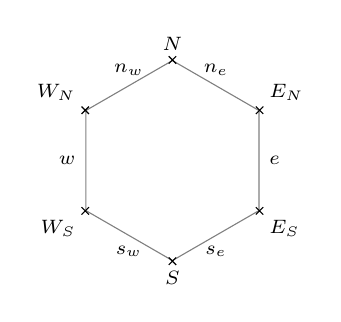
\begin{tikzpicture}[scale=1,transform shape]
%\draw [dashed] (0,0) rectangle (3, -3);
\node (h) [draw, color=gray, shape border rotate=30, minimum size=1in, regular polygon, regular polygon sides=6] at (0,0) {};



\foreach \anchor/\placement/\label in
    {corner 1/above/$N$, corner 2/above left/$W_N$, corner 3/below left/$W_S$, corner 4/below/$S$, corner 5/below right/$E_S$, corner 6/above right/$E_N$}
\draw[shift=(h.\anchor)] plot[mark=x,mark size=1.9pt] coordinates{(0,0)} 
node [\placement] {{\scriptsize\label}};

\foreach \anchor/\placement/\label in
    {side 1/above/$n_w$, side 2/left/$w$, side 3/below/$s_w$, side 4/below/$s_e$, side 5/right/$e$, side 6/above/$n_e$}
\draw[shift=(h.\anchor)] plot coordinates{(0,0)} 
node [\placement] {{\scriptsize\label}};

\end{tikzpicture}\hspace{1cm}
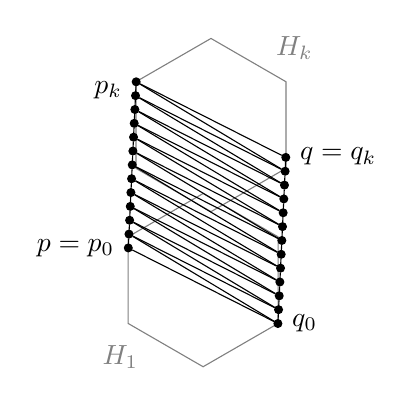
\begin{tikzpicture}[scale=2]

%\draw [color=gray] (0,0) -- (0, 1.22) -- (2.15, 1.22) -- node [right] {\scriptsize $y$}(2.15, 0) -- (0, 0);
\node [draw, color=gray, shape border rotate=30, minimum size=2.2cm, regular polygon, regular polygon sides=6,label=-135:{{\color{gray}{$H_1$}}}] at (0.475,-.2044) (H) {};
\node [draw, color=gray, shape border rotate=30, minimum size=2.2cm, regular polygon, regular polygon sides=6,label=45:{{\color{gray}{$H_k$}}}] at (0.525,.7803) (H) {};


\node at (0, 0) [draw,fill, inner sep = 1pt, circle, label=180:{$p=p_0$}] (h) {};
\node at (0.95, -0.48) [draw,fill, inner sep = 1pt, circle, label=0:{$q_0$}] (l) {};

\draw (h) -- (l);

\foreach \x in {1, ..., 12}
{
  \node at (\x*0.004167, \x*0.0879) [draw, fill, inner sep = 1pt, circle] (h) {};
  \draw (h) -- (l);
  \draw (h) -- (\x*0.004167-0.004167, \x*0.0879-0.0879);
  \node at (\x*0.004167+0.95, \x*0.0879-0.48) [draw,fill, inner sep = 1pt, circle] (l) {};
  \draw (h) -- (l);
  \draw (l) -- (\x*0.004167-0.004167+0.95, \x*0.0879-0.0879-0.48);
}

\node at (0.05, 1) [inner sep = 1pt, circle, label=180:{$p_k$}] {};
\node at (1, 0.58) [inner sep = 1pt, circle, label=0:{$q=q_k$}] (h) {};
%\draw (h) -- (l);

%\draw [color=gray, dashed] (0.15, 3) -- (0.15, 1) -- (2.15, 1) -- (2.15, 3) -- node [below] {\scriptsize $1-\delta$} (0.15, 3);

%\draw [color=gray, dashed] (c2) -- node [above] {\scriptsize $1-\delta$} (0, -1.8) -- (0, 0.2) -- (2.01, 0.2) -- (c2);

\end{tikzpicture}\hspace{0.5cm}
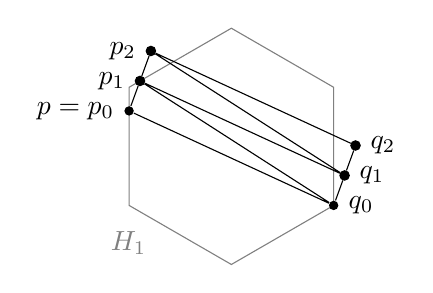
\begin{tikzpicture}[scale=1.5]
%\draw [dashed] (0,0) rectangle (3, -3);
\node [draw, color=gray, shape border rotate=30, minimum size=1.18125in, regular polygon, regular polygon sides=6,label=-135:{{\color{gray}{$H_1$}}}] at (0.866025,-.5) (H) {};


\node at (0,-0.2) [fill, circle, inner sep=1.2pt, label=180:{$p=p_0$}] (a) {};
\path (a) ++(70:0.27) node (p1) [draw,circle,inner sep=1.2pt,fill=black,label=180:$p_1$] {};
\path [draw] (p1) ++(70:0.27) node (p2) [draw,circle,inner sep=1.2pt,fill=black,label=180:$p_2$] {};


\node at (1.73205,-1) [fill, circle, inner sep=1.2pt, label=0:$q_0$] (c2) {};
\path (c2) ++(70:0.27) node (q1) [draw,circle,inner sep=1.2pt,fill=black,label=0:$q_1$] {};
\path (q1) ++(70:0.27) node (q2) [draw,circle,inner sep=1.2pt,fill=black,label=0:$q_2$] {};

\draw (p2) -- (p1) -- (a) -- (c2) -- (p1) -- (q1) -- (p2) -- (q2) -- (q1) -- (c2);

%\draw [color=gray, dashed] (0,0) -- (3,0) -- (3, -3) -- node [below] {\scriptsize $1-\delta$} (0,-3) -- (0, 0);
%\node at (3.2, 0.2) [] {\color{gray}{$S_1$}};
%\draw [dashed] (0.25,0) rectangle (3.25, -3);
%\draw [color=gray, dashed] (0.25,0.7) rectangle (3.25, -2.3);

%\node at (3.25,-2.3) [fill, circle, inner sep=2pt, label=0:$q_1$] (q) {};
%\node at (0.25,0) [fill, circle, inner sep=2pt, label=115:$p_1$] (p1) {};
%\node at (0.5,0.7) [fill, circle, inner sep=2pt, label=115:$p_2$] (p2) {};

%\draw (q) -- (p2) -- (p1) -- (c2) -- (q) -- (p1) -- (a) -- (c2);

%\node at (-0.24,-0.24) [color=gray] {{\small $\delta$}};
\end{tikzpicture}
}


\newcommand{\regular}{
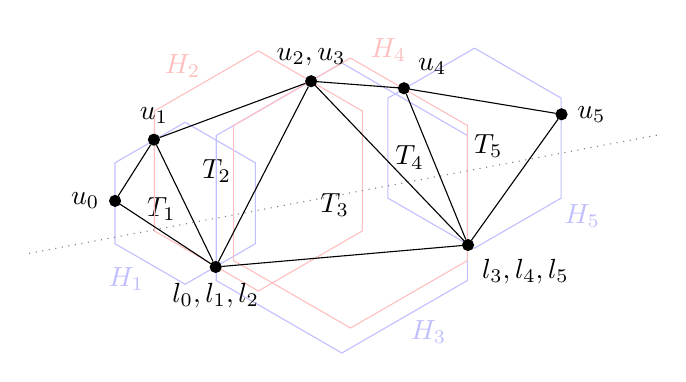
\begin{tikzpicture}[scale=1, transform shape]
\clip (0,-1.14) rectangle (8,3);


\node [color=red!25, shape border rotate=30, minimum size=0.7in, regular polygon, regular polygon sides=6] at (0,0.33) (Hm3) {};

\node [color=blue!25, shape border rotate=30, minimum size=0.58in, regular polygon, regular polygon sides=6] at (0.47,0.45) (Hm2) {};

\node [color=red!25, shape border rotate=30, minimum size=0.78in, regular polygon, regular polygon sides=6] at (1.53,-0.05) (Hm1) {};

\node [draw, color=blue!25, shape border rotate=30, minimum size=0.81in, regular polygon, regular polygon sides=6, label={[label distance=-0.1cm]-120:{\color{blue!25}{$H_1$}}}] at (2,0.77) (H1) {};

\node at (1.7,0.7) {$T_1$};

%\node [draw,color=blue!25, shape border rotate=30, minimum size=0.8in, regular polygon, regular polygon sides=6] at (1.73,0.61) (H1) {};

\node [draw, color=red!25, shape border rotate=30, minimum size=1.2in, regular polygon, regular polygon sides=6, label={[label distance=-0.1cm]120:{\color{red!25}{$H_2$}}}] at (2.93,1.18) (H2) {};

\node at (2.4,1.18) {$T_2$};

\node [draw,color=blue!25, shape border rotate=30, minimum size=1.45in, regular polygon, regular polygon sides=6, label={[label distance=-0.1cm]-60:{\color{blue!25}{$H_3$}}}] at (3.99,0.71) (H3) {};

\node at (3.9,0.75) {$T_3$};

\node [draw, color=red!25, shape border rotate=30, minimum size=1.35in, regular polygon, regular polygon sides=6, label={[label distance=-0.1cm]85:{\color{red!25}{$H_4$}}}] at (4.1,0.9) (H4) {};

\node at (4.85,1.35) {$T_4$};

\node [draw, color=blue!25, shape border rotate=30, minimum size=1in, regular polygon, regular polygon sides=6, label={[label distance=-0.1cm]-30:{\color{blue!25}{$H_5$}}}] at (5.675,1.47) (H5) {};

\node at (5.85,1.5) {$T_5$};

\node [color=red!25, shape border rotate=30, minimum size=1.43in, regular polygon, regular polygon sides=6] at (6.06,3.3) (H6) {};

\node [color=blue!25, shape border rotate=30, minimum size=1.6in, regular polygon, regular polygon sides=6] at (6.25,3.625) (H7) {};

\node [color=red!25, shape border rotate=30, minimum size=1.355in, regular polygon, regular polygon sides=6] at (7.24,3.36) (H8) {};

\node [color=blue!25, shape border rotate=30, minimum size=1.45in, regular polygon, regular polygon sides=6] at (7.6,3.27) (H9) {};

\node [color=red!25, shape border rotate=30, minimum size=1.45in, regular polygon, regular polygon sides=6] at (8,3.5) (H10) {};

\node at (Hm3.side 3) [yshift=.4cm,circle,inner sep=1.4pt] (s) {};

\node at (H10.side 6) [yshift=-3.1cm,circle,inner sep=1.4pt] (t) {};

%\node at (10,3.333) [draw,fill,circle,inner sep=1.4pt,label=180:{$t$}] (t) {};
\draw [gray, dotted] (s) -- (t);

\node at (Hm3.corner 6) (a) {};
\node at (Hm3.corner 1) (b) {};
\node at (Hm2.corner 1) (c) {};
\node at (Hm2.corner 2) (d) {};

\node at (intersection of a--b and c--d) [circle,inner sep=1.4pt] (h1) {};

\node at (Hm2.corner 4) (a) {};
\node at (Hm2.corner 5) (b) {};
\node at (Hm1.corner 2) (c) {};
\node at (Hm1.corner 3) (d) {};

\node at (intersection of a--b and c--d) [circle,inner sep=1.4pt] (l1) {};

\node at (1.11,0.8) [draw,fill,circle,inner sep=1.4pt,label=180:{$u_0$}] (h2) {};

\node at (H1.corner 1) (a) {};
\node at (H1.corner 2) (b) {};
\node at (H2.corner 2) (c) {};
\node at (H2.corner 3) (d) {};

\node at (intersection of a--b and c--d) [draw,fill,circle,inner sep=1.4pt,label=90:{$u_1$}] (h4) {};

\node at (H2.corner 3) (a) {};
\node at (H2.corner 4) (b) {};
\node at (H3.corner 2) (c) {};
\node at (H3.corner 3) (d) {};

\node at (intersection of a--b and c--d) [draw,fill,circle,inner sep=1.4pt,label=-90:{$l_0,l_1,l_2$}] (l3) {};

\node at (3.6,2.32) [draw,fill,circle,inner sep=1.4pt,label=90:{$u_2,u_3$}] (h5) {};

\node at (H4.corner 6) (a) {};
\node at (H4.corner 1) (b) {};
\node at (H5.corner 1) (c) {};
\node at (H5.corner 2) (d) {};

\node at (intersection of a--b and c--d) [draw,fill,circle,inner sep=1.4pt,label=45:{$u_4$}] (h7) {};

\node at (H4.corner 5) (a) {};
\node at (H4.corner 6) (b) {};
\node at (H5.corner 3) (c) {};
\node at (H5.corner 4) (d) {};

\node at (intersection of a--b and c--d) [draw,fill,circle,inner sep=1.4pt,label=-45:{$l_3,l_4,l_5$}] (l6) {};

\node at (6.78,1.9) [draw,fill,circle,inner sep=1.4pt,label=0:{$u_5$}] (l8) {};

\node at (4.48,3.6) [circle,inner sep=1.4pt] (h9) {};

\node at (H8.corner 6) (a) {};
\node at (H8.corner 1) (b) {};
\node at (H9.corner 1) (c) {};
\node at (H9.corner 2) (d) {};

\node at (intersection of a--b and c--d) [circle,inner sep=1.4pt] (h10) {};

\node at (8.34,1.85) [circle,inner sep=1.4pt] (l11) {};


\draw (l3) -- (h2) -- (h4) -- (l3) -- (h5) -- (h4);
\draw (l3) -- (l6) -- (h5) -- (h7) -- (l6) -- (l8) -- (h7); 

\node (tmp) at ($(h7)+(150:5)$) {};
\node (tmp2) at ($(h2)+(90:4)$) {};

\coordinate (z) at (intersection of h7--tmp and h2--tmp2);

%\draw [dashed, red] (h2) -- (z) -- (h7);

\node (tmp) at ($(h7)+(330:5)$) {};
\node (tmp2) at ($(l11)+(270:4)$) {};

\coordinate (z) at (intersection of h7--tmp and l11--tmp2);

%\draw [dashed, red] (l11) -- (z) -- (h7);



\end{tikzpicture}
}



\newcommand{\discretedNdS}{
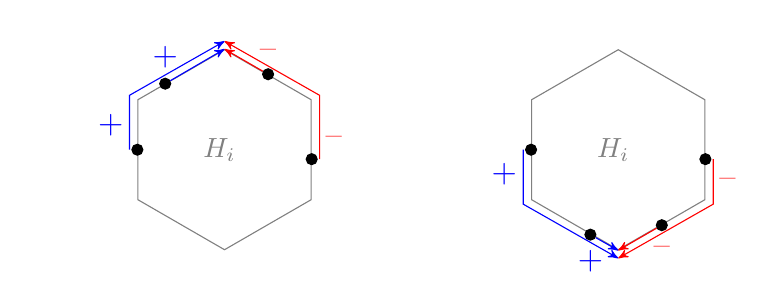
\begin{tikzpicture}[scale=1]
\clip (-2.5,-1.55) rectangle (6.5,1.55);
\node (h) [draw, color=gray, shape border rotate=30, minimum size=1in, regular polygon, regular polygon sides=6,label={[label distance=-1.5cm]0:{\color{gray}{$H_i$}}}] at (0,0) {};

\node at (h.side 1) [xshift=-0.2cm,yshift=-0.12cm,draw,circle,fill,inner sep=1.4pt,label=90:{\color{blue}{\large +}}] (s1) {};
\node at (h.side 2) [draw,circle,fill,inner sep=1.4pt,label=135:{\color{blue}{\large +}}] (s2) {};
%\node at (h.side 3) [xshift=+0.2cm,yshift=-0.12cm,draw,circle,fill,inner sep=1.4pt,label=90:{\color{blue}{\large +}}] (s3) {};

\draw (s1) -- (h.corner 1) [->,>=stealth',blue,label=-45:{$+$}];
\draw ($(s2) + (-0.1cm,0)$) -- ($(h.corner 2) + (-0.1cm,0.052cm)$) -- ($(h.corner 1) + (0,0.1cm)$) [->,>=stealth',blue,label=-45:{$+$}];
%\draw ($(s3) + (0.052cm,0.1cm)$) -- ($(h.corner 3) + (0.1cm,0.052cm)$) -- ($(h.corner 2) + (0.1cm,-0.052cm)$) -- ($(h.corner 1) + (0,-0.1cm)$) [->,>=stealth',blue,label=-45:{$+$}];

\node at (h.side 6) [draw,circle,fill,inner sep=1.4pt,label=90:{\color{red}{\large --}}] (s1) {};
\node at (h.side 5) [yshift=-0.12cm,draw,circle,fill,inner sep=1.4pt,label=45:{\color{red}{\large --}}] (s2) {};
%\node at (h.side 4) [draw,circle,fill,inner sep=1.4pt,label=90:{\color{red}{\large --}}] (s3) {};

\draw (s1) -- (h.corner 1) [->,>=stealth',red];
\draw ($(s2) + (0.1cm,0)$) -- ($(h.corner 6) + (0.1cm,0.052cm)$) -- ($(h.corner 1) + (0,0.1cm)$) [->,>=stealth',red];
%\draw ($(s3) + (-0.052,0.1cm)$) -- ($(h.corner 5) + (-0.1cm,0.052cm)$) -- ($(h.corner 6) + (-0.1cm,-0.052cm)$) -- ($(h.corner 1) + (0,-0.1cm)$) [->,>=stealth',red];

\node (h) [draw, color=gray, shape border rotate=30, minimum size=1in, regular polygon, regular polygon sides=6,label={[label distance=-1.5cm]0:{\color{gray}{$H_i$}}}] at (5,0) {};

%\node at (h.side 1) [xshift=-0.2cm,yshift=-0.12cm,draw,circle,fill,inner sep=1.4pt,label=-90:{\color{blue}{\large +}}] (s1) {};
\node at (h.side 2) [draw,circle,fill,inner sep=1.4pt,label=-135:{\color{blue}{\large +}}] (s2) {};
\node at (h.side 3) [xshift=+0.2cm,yshift=-0.12cm,draw,circle,fill,inner sep=1.4pt,label=-90:{\color{blue}{\large +}}] (s3) {};

\draw (s3) -- (h.corner 4) [->,>=stealth',blue,label=-45:{$+$}];
\draw ($(s2) + (-0.1cm,0)$) -- ($(h.corner 3) + (-0.1cm,-0.052cm)$) -- ($(h.corner 4) + (0,-0.1cm)$) [->,>=stealth',blue,label=-45:{$+$}];
%\draw ($(s1) + (0.052cm,-0.09cm)$) -- ($(h.corner 2) + (0.1cm,-0.052cm)$) -- ($(h.corner 3) + (0.1cm,0.052cm)$) -- ($(h.corner 4) + (0,0.1cm)$) [->,>=stealth',blue,label=-45:{$+$}];

%\node at (h.side 6) [draw,circle,fill,inner sep=1.4pt,label=-90:{\color{red}{\large --}}] (s1) {};
\node at (h.side 5) [yshift=-0.12cm,draw,circle,fill,inner sep=1.4pt,label=-45:{\color{red}{\large --}}] (s2) {};
\node at (h.side 4) [draw,circle,fill,inner sep=1.4pt,label=-90:{\color{red}{\large --}}] (s3) {};

\draw (s3) -- (h.corner 4) [->,>=stealth',red];
\draw ($(s2) + (0.1cm,0)$) -- ($(h.corner 5) + (0.1cm,-0.052cm)$) -- ($(h.corner 4) + (0,-0.1cm)$) [->,>=stealth',red];
%\draw ($(s1) + (-0.052,-0.1cm)$) -- ($(h.corner 6) + (-0.1cm,-0.052cm)$) -- ($(h.corner 5) + (-0.1cm,0.052cm)$) -- ($(h.corner 4) + (0,0.1cm)$) [->,>=stealth',red];
\end{tikzpicture}\hspace{1.34cm}
\begin{tikzpicture}[scale=1]
\clip (-2.35,-1.45) rectangle (6.5,1.65);
\node (h) [draw, color=gray, shape border rotate=30, minimum size=1in, regular polygon, regular polygon sides=6,label={[label distance=-1.5cm]0:{\color{gray}{$H_i$}}}] at (0,0) {};

\node at (h.side 2) [draw,circle,fill,inner sep=1.4pt,label=180:{$u_{i-1}$}] (uj) {};
\node at (h.side 6) [draw,circle,fill,inner sep=1.4pt,label=0:{$u_i$}] (ujp) {};

\draw (uj) -- (h.corner 2) -- (h.corner 1) [->,>=stealth',blue];
\draw (ujp) -- (h.corner 1) [->,>=stealth',red];

\draw (uj) -- (ujp);

\node at (-1.45,1.1) [blue] {$p_N(u_{i-1},i)$};
\node at (1.05,1.45) [red] {$p_N(u_i,i)$};
\end{tikzpicture}
}



\newcommand{\definitions}{
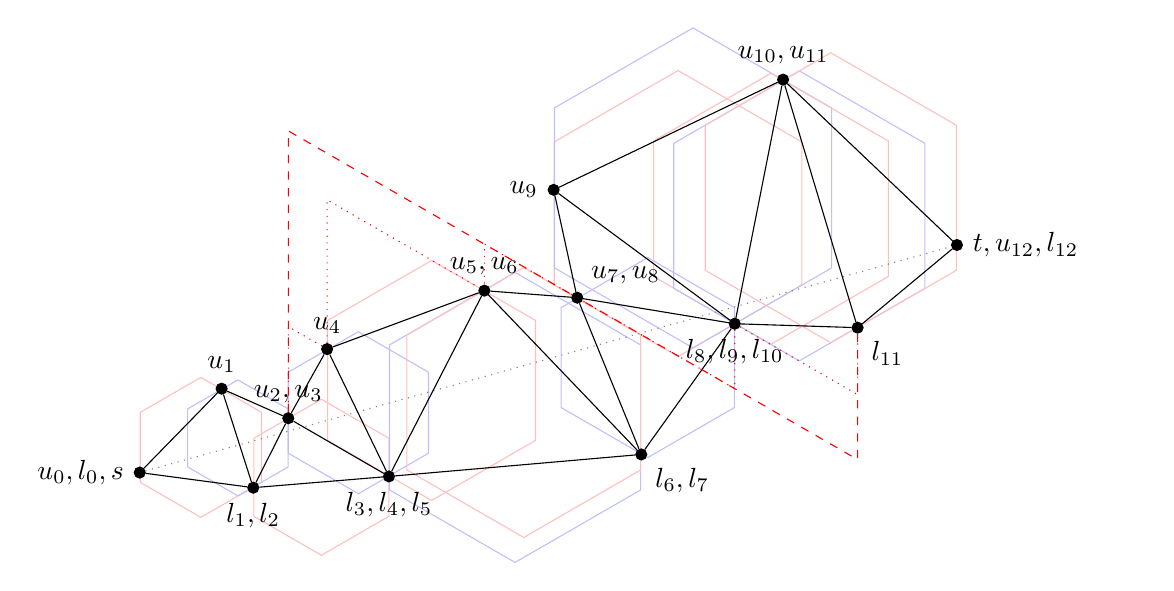
\begin{tikzpicture}[scale=1, transform shape]
\clip (-2.2,-1.14) rectangle (12,5.66);


\node [draw, color=red!25, shape border rotate=30, minimum size=0.7in, regular polygon, regular polygon sides=6] at (0,0.33) (Hm3) {};

\node [draw, color=blue!25, shape border rotate=30, minimum size=0.58in, regular polygon, regular polygon sides=6] at (0.47,0.45) (Hm2) {};

\node [draw,color=red!25, shape border rotate=30, minimum size=0.78in, regular polygon, regular polygon sides=6] at (1.53,-0.05) (Hm1) {};

\node [draw, color=blue!25, shape border rotate=30, minimum size=0.81in, regular polygon, regular polygon sides=6] at (2,0.77) (H1) {};

%\node [draw,color=blue!25, shape border rotate=30, minimum size=0.8in, regular polygon, regular polygon sides=6] at (1.73,0.61) (H1) {};

\node [draw, color=red!25, shape border rotate=30, minimum size=1.2in, regular polygon, regular polygon sides=6] at (2.93,1.18) (H2) {};

\node [draw,color=blue!25, shape border rotate=30, minimum size=1.45in, regular polygon, regular polygon sides=6] at (3.99,0.71) (H3) {};

\node [draw, color=red!25, shape border rotate=30, minimum size=1.35in, regular polygon, regular polygon sides=6] at (4.1,0.9) (H4) {};

\node [draw, color=blue!25, shape border rotate=30, minimum size=1in, regular polygon, regular polygon sides=6] at (5.675,1.47) (H5) {};

\node [draw,color=red!25, shape border rotate=30, minimum size=1.43in, regular polygon, regular polygon sides=6] at (6.06,3.3) (H6) {};

\node [draw,color=blue!25, shape border rotate=30, minimum size=1.6in, regular polygon, regular polygon sides=6] at (6.25,3.625) (H7) {};

\node [draw,color=red!25, shape border rotate=30, minimum size=1.355in, regular polygon, regular polygon sides=6] at (7.24,3.36) (H8) {};

\node [draw,color=blue!25, shape border rotate=30, minimum size=1.45in, regular polygon, regular polygon sides=6] at (7.6,3.27) (H9) {};

\node [draw, color=red!25, shape border rotate=30, minimum size=1.45in, regular polygon, regular polygon sides=6] at (8,3.5) (H10) {};



\node at (Hm3.side 2) [yshift=-0.32cm,draw,circle,fill,inner sep=1.4pt,label=180:{$u_0,l_0,s$}] (s) {};

\node at (H10.side 5) [yshift=-0.6cm,draw,circle,fill,inner sep=1.4pt,label=0:{$t,u_{12},l_{12}$}] (t) {};

%\node at (10,3.333) [draw,fill,circle,inner sep=1.4pt,label=180:{$t$}] (t) {};
\draw [gray, dotted] (s) -- (t);

\node at (Hm3.corner 6) (a) {};
\node at (Hm3.corner 1) (b) {};
\node at (Hm2.corner 1) (c) {};
\node at (Hm2.corner 2) (d) {};

\node at (intersection of a--b and c--d) [draw,fill,circle,inner sep=1.4pt,label=90:{$u_1$}] (h1) {};

\node at (Hm2.corner 4) (a) {};
\node at (Hm2.corner 5) (b) {};
\node at (Hm1.corner 2) (c) {};
\node at (Hm1.corner 3) (d) {};

\node at (intersection of a--b and c--d) [draw,fill,circle,inner sep=1.4pt,label=-90:{$l_1,l_2$}] (l1) {};

\node at (1.11,0.7) [draw,fill,circle,inner sep=1.4pt,label=90:{$u_2,u_3$}] (h2) {};

\node at (H1.corner 1) (a) {};
\node at (H1.corner 2) (b) {};
\node at (H2.corner 2) (c) {};
\node at (H2.corner 3) (d) {};

\node at (intersection of a--b and c--d) [draw,fill,circle,inner sep=1.4pt,label=90:{$u_4$}] (h4) {};

\node at (H2.corner 3) (a) {};
\node at (H2.corner 4) (b) {};
\node at (H3.corner 2) (c) {};
\node at (H3.corner 3) (d) {};

\node at (intersection of a--b and c--d) [draw,fill,circle,inner sep=1.4pt,label=-90:{$l_3,l_4,l_5$}] (l3) {};

\node at (3.6,2.32) [draw,fill,circle,inner sep=1.4pt,label=90:{$u_5,u_6$}] (h5) {};

\node at (H4.corner 6) (a) {};
\node at (H4.corner 1) (b) {};
\node at (H5.corner 1) (c) {};
\node at (H5.corner 2) (d) {};

\node at (intersection of a--b and c--d) [draw,fill,circle,inner sep=1.4pt,label=45:{$u_7,u_8$}] (h7) {};

\node at (H4.corner 5) (a) {};
\node at (H4.corner 6) (b) {};
\node at (H5.corner 3) (c) {};
\node at (H5.corner 4) (d) {};

\node at (intersection of a--b and c--d) [draw,fill,circle,inner sep=1.4pt,label=-45:{$l_6,l_7$}] (l6) {};

\node at (6.78,1.9) [draw,fill,circle,inner sep=1.4pt,label=-90:{$l_8,l_9,l_{10}$}] (l8) {};

\node at (4.48,3.6) [draw,fill,circle,inner sep=1.4pt,label=180:{$u_9$}] (h9) {};

\node at (H8.corner 6) (a) {};
\node at (H8.corner 1) (b) {};
\node at (H9.corner 1) (c) {};
\node at (H9.corner 2) (d) {};

\node at (intersection of a--b and c--d) [draw,fill,circle,inner sep=1.4pt,label=90:{$u_{10},u_{11}$}] (h10) {};

\node at (8.34,1.85) [draw,fill,circle,inner sep=1.4pt,label=-45:{$l_{11}$}] (l11) {};


\draw (h1) -- (s) -- (l1) -- (h1) -- (h2) -- (l1) -- (l3) -- (h2) -- (h4) -- (l3) -- (h5) -- (h4);
\draw (l3) -- (l6) -- (h5) -- (h7) -- (l6) -- (l8) -- (h7) -- (h9) -- (l8) -- (h10) -- (h9);
\draw (l8) -- (l11) -- (h10) -- (t) -- (l11); 

\node (tmp) at ($(h7)+(150:5)$) {};
\node (tmp2) at ($(h2)+(90:4)$) {};

\coordinate (z) at (intersection of h7--tmp and h2--tmp2);

\draw [dashed, red] (h2) -- (z) -- (h7);


\node (tmp) at ($(h4)+(150:5)$) {};
\coordinate (z) at (intersection of h4--tmp and h2--tmp2);
\draw [dotted, red] (h4) -- (z) -- (h2);

\node (tmp) at ($(h5)+(150:5)$) {};
\node (tmp2) at ($(h4)+(90:5)$) {};
\coordinate (z) at (intersection of h5--tmp and h4--tmp2);
\draw [dotted, red] (h4) -- (z) -- (h5);

\node (tmp) at ($(h7)+(150:5)$) {};
\node (tmp2) at ($(h5)+(90:5)$) {};
\coordinate (z) at (intersection of h7--tmp and h5--tmp2);
\draw [dotted, red] (h7) -- (z) -- (h5);




%%%%%%

\node (tmp) at ($(h7)+(330:5)$) {};
\node (tmp2) at ($(l11)+(270:4)$) {};

\coordinate (z) at (intersection of h7--tmp and l11--tmp2);

\draw [dashed, red] (l11) -- (z) -- (h7);


\node (tmp2) at ($(l8)+(270:5)$) {};
\coordinate (z) at (intersection of h7--tmp and l8--tmp2);
\draw [dotted, red] (l8) -- (z) -- (h7);

\node (tmp) at ($(l8)+(330:5)$) {};
\node (tmp2) at ($(l11)+(270:5)$) {};
\coordinate (z) at (intersection of l8--tmp and l11--tmp2);
\draw [dotted, red] (l8) -- (z) -- (l11);




\end{tikzpicture}
}




\newcommand{\infity}{
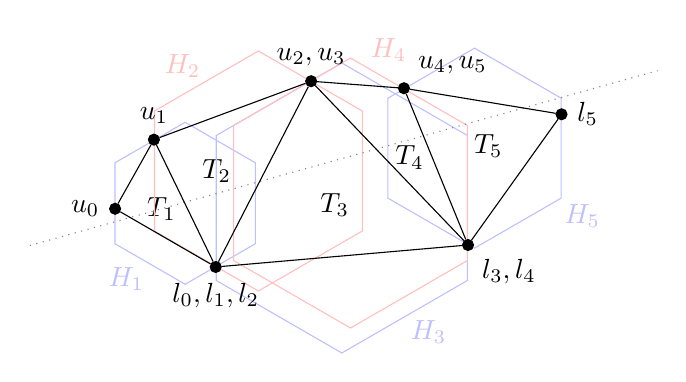
\begin{tikzpicture}[scale=1, transform shape]
\clip (0,-1.14) rectangle (8,3);


\node [color=red!25, shape border rotate=30, minimum size=0.7in, regular polygon, regular polygon sides=6] at (0,0.33) (Hm3) {};

\node [color=blue!25, shape border rotate=30, minimum size=0.58in, regular polygon, regular polygon sides=6] at (0.47,0.45) (Hm2) {};

\node [color=red!25, shape border rotate=30, minimum size=0.78in, regular polygon, regular polygon sides=6] at (1.53,-0.05) (Hm1) {};

\node [draw, color=blue!25, shape border rotate=30, minimum size=0.81in, regular polygon, regular polygon sides=6, label={[label distance=-0.1cm]-120:{\color{blue!25}{$H_1$}}}] at (2,0.77) (H1) {};

\node at (1.7,0.7) {$T_1$};

%\node [draw,color=blue!25, shape border rotate=30, minimum size=0.8in, regular polygon, regular polygon sides=6] at (1.73,0.61) (H1) {};

\node [draw, color=red!25, shape border rotate=30, minimum size=1.2in, regular polygon, regular polygon sides=6, label={[label distance=-0.1cm]120:{\color{red!25}{$H_2$}}}] at (2.93,1.18) (H2) {};

\node at (2.4,1.18) {$T_2$};

\node [draw,color=blue!25, shape border rotate=30, minimum size=1.45in, regular polygon, regular polygon sides=6, label={[label distance=-0.1cm]-60:{\color{blue!25}{$H_3$}}}] at (3.99,0.71) (H3) {};

\node at (3.9,0.75) {$T_3$};

\node [draw, color=red!25, shape border rotate=30, minimum size=1.35in, regular polygon, regular polygon sides=6, label={[label distance=-0.1cm]85:{\color{red!25}{$H_4$}}}] at (4.1,0.9) (H4) {};

\node at (4.85,1.35) {$T_4$};

\node [draw, color=blue!25, shape border rotate=30, minimum size=1in, regular polygon, regular polygon sides=6, label={[label distance=-0.1cm]-30:{\color{blue!25}{$H_5$}}}] at (5.675,1.47) (H5) {};

\node at (5.85,1.5) {$T_5$};

\node [color=red!25, shape border rotate=30, minimum size=1.43in, regular polygon, regular polygon sides=6] at (6.06,3.3) (H6) {};

\node [color=blue!25, shape border rotate=30, minimum size=1.6in, regular polygon, regular polygon sides=6] at (6.25,3.625) (H7) {};

\node [color=red!25, shape border rotate=30, minimum size=1.355in, regular polygon, regular polygon sides=6] at (7.24,3.36) (H8) {};

\node [color=blue!25, shape border rotate=30, minimum size=1.45in, regular polygon, regular polygon sides=6] at (7.6,3.27) (H9) {};

\node [color=red!25, shape border rotate=30, minimum size=1.45in, regular polygon, regular polygon sides=6] at (8,3.5) (H10) {};

\node at (Hm3.side 2) [yshift=-0.32cm,circle,inner sep=1.4pt] (s) {};

\node at (H10.side 5) [yshift=-0.6cm,circle,inner sep=1.4pt] (t) {};

\draw [gray, dotted] (s) -- (t);

\node at (Hm3.corner 6) (a) {};
\node at (Hm3.corner 1) (b) {};
\node at (Hm2.corner 1) (c) {};
\node at (Hm2.corner 2) (d) {};

\node at (intersection of a--b and c--d) [circle,inner sep=1.4pt] (h1) {};

\node at (Hm2.corner 4) (a) {};
\node at (Hm2.corner 5) (b) {};
\node at (Hm1.corner 2) (c) {};
\node at (Hm1.corner 3) (d) {};

\node at (intersection of a--b and c--d) [circle,inner sep=1.4pt] (l1) {};

\node at (1.11,0.7) [draw,fill,circle,inner sep=1.4pt,label=180:{$u_0$}] (h2) {};

\node at (H1.corner 1) (a) {};
\node at (H1.corner 2) (b) {};
\node at (H2.corner 2) (c) {};
\node at (H2.corner 3) (d) {};

\node at (intersection of a--b and c--d) [draw,fill,circle,inner sep=1.4pt,label=90:{$u_1$}] (h4) {};

\node at (H2.corner 3) (a) {};
\node at (H2.corner 4) (b) {};
\node at (H3.corner 2) (c) {};
\node at (H3.corner 3) (d) {};

\node at (intersection of a--b and c--d) [draw,fill,circle,inner sep=1.4pt,label=-90:{$l_0,l_1,l_2$}] (l3) {};

\node at (3.6,2.32) [draw,fill,circle,inner sep=1.4pt,label=90:{$u_2,u_3$}] (h5) {};

\node at (H4.corner 6) (a) {};
\node at (H4.corner 1) (b) {};
\node at (H5.corner 1) (c) {};
\node at (H5.corner 2) (d) {};

\node at (intersection of a--b and c--d) [draw,fill,circle,inner sep=1.4pt,label=45:{$u_4,u_5$}] (h7) {};

\node at (H4.corner 5) (a) {};
\node at (H4.corner 6) (b) {};
\node at (H5.corner 3) (c) {};
\node at (H5.corner 4) (d) {};

\node at (intersection of a--b and c--d) [draw,fill,circle,inner sep=1.4pt,label=-45:{$l_3,l_4$}] (l6) {};

\node at (6.78,1.9) [draw,fill,circle,inner sep=1.4pt,label=0:{$l_5$}] (l8) {};

\node at (4.48,3.6) [circle,inner sep=1.4pt] (h9) {};

\node at (H8.corner 6) (a) {};
\node at (H8.corner 1) (b) {};
\node at (H9.corner 1) (c) {};
\node at (H9.corner 2) (d) {};

\node at (intersection of a--b and c--d) [circle,inner sep=1.4pt] (h10) {};

\node at (8.34,1.85) [circle,inner sep=1.4pt] (l11) {};


\draw (l3) -- (h2) -- (h4) -- (l3) -- (h5) -- (h4);
\draw (l3) -- (l6) -- (h5) -- (h7) -- (l6) -- (l8) -- (h7); 

\node (tmp) at ($(h7)+(150:5)$) {};
\node (tmp2) at ($(h2)+(90:4)$) {};

\coordinate (z) at (intersection of h7--tmp and h2--tmp2);

%\draw [dashed, red] (h2) -- (z) -- (h7);

\node (tmp) at ($(h7)+(330:5)$) {};
\node (tmp2) at ($(l11)+(270:4)$) {};

\coordinate (z) at (intersection of h7--tmp and l11--tmp2);

%\draw [dashed, red] (l11) -- (z) -- (h7);



\end{tikzpicture}
}

\newcommand{\infinity}{
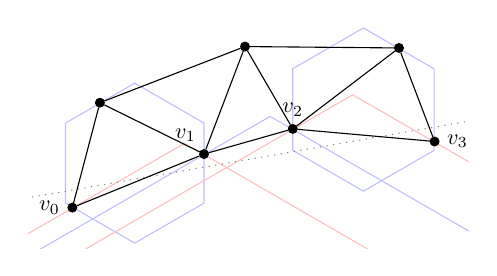
\begin{tikzpicture}[scale=.8, transform shape]
\clip (-0.2,-0.2) rectangle (6.8,3.3);


\node [draw, color=blue!25, shape border rotate=30, minimum size=1in, regular polygon, regular polygon sides=6] at (1.5,1.15) (H1) {};

\node [draw, color=red!25, shape border rotate=30, minimum size=3.2in, regular polygon, regular polygon sides=6] at (2.29,-2.6) (H2) {};

\node [draw,color=blue!25, shape border rotate=30, minimum size=4.45in, regular polygon, regular polygon sides=6] at (3.65,-3.76) (H3) {};

\node [draw, color=red!25, shape border rotate=30, minimum size=5.35in, regular polygon, regular polygon sides=6] at (4.96,-4.56) (H4) {};

\node [draw, color=blue!25, shape border rotate=30, minimum size=1.02in, regular polygon, regular polygon sides=6] at (5.13,2) (H5) {};

\node at (H1.corner 3) [xshift=-1.1cm,inner sep=1.4pt,label=180:{$s$}] (s) {};

\node at (H5.side 5) [xshift=+1.6cm,yshift=+0cm,inner sep=1.4pt,label=0:{$t,u_{12},l_{12}$}] (t) {};

\draw [gray, dotted] (s) -- (t);

\node at (H1.corner 3) (a) {};
\node at (H1.corner 4) (b) {};
\node at (H2.corner 1) (c) {};
\node at (H2.corner 2) (d) {};

\node at (intersection of a--b and c--d) [draw,fill,circle,inner sep=1.4pt,label=180:{$v_0$}] (v0) {};

\node at (H2.corner 1) (a) {};
\node at (H2.corner 6) (b) {};
\node at (H3.corner 1) (c) {};
\node at (H3.corner 2) (d) {};

\node at (intersection of a--b and c--d) [draw,fill,circle,inner sep=1.4pt,label=94:{$v_1$}] (v1) {};

\node at (H3.corner 1) (a) {};
\node at (H3.corner 6) (b) {};
\node at (H4.corner 1) (c) {};
\node at (H4.corner 2) (d) {};

\node at (intersection of a--b and c--d) [draw,fill,circle,inner sep=1.4pt,label=92:{$v_2$}] (v2) {};

\node at (H4.corner 1) (a) {};
\node at (H4.corner 6) (b) {};
\node at (H5.corner 5) (c) {};
\node at (H5.corner 6) (d) {};

\node at (intersection of a--b and c--d) [draw,fill,circle,inner sep=1.4pt,label=0:{$v_3$}] (v3) {};

\node at (H1.side 1) [draw,fill,circle,inner sep=1.4pt] (v) {};
\node at (H5.side 6) [draw,fill,circle,inner sep=1.4pt] (w) {};

\node at (3.25,3) [draw,fill,circle,inner sep=1.4pt] (u) {};


\draw (v1) -- (v) -- (v0) -- (v1) -- (v2) -- (v3) -- (w) -- (v2);

\draw (v) -- (u) -- (w); 
\draw (v1) -- (u) -- (v2); 

\end{tikzpicture}\hspace{1.5cm}
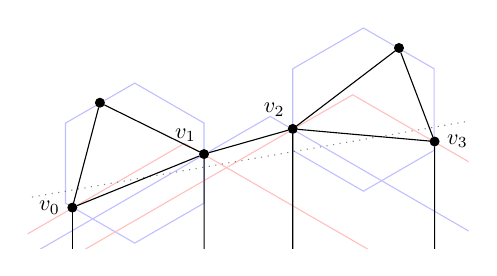
\begin{tikzpicture}[scale=.8, transform shape]
\clip (-0.2,-0.2) rectangle (6.8,3.3);


\node [draw, color=blue!25, shape border rotate=30, minimum size=1in, regular polygon, regular polygon sides=6] at (1.5,1.15) (H1) {};

\node [draw, color=red!25, shape border rotate=30, minimum size=3.2in, regular polygon, regular polygon sides=6] at (2.29,-2.6) (H2) {};

\node [draw,color=blue!25, shape border rotate=30, minimum size=4.45in, regular polygon, regular polygon sides=6] at (3.65,-3.76) (H3) {};

\node [draw, color=red!25, shape border rotate=30, minimum size=5.35in, regular polygon, regular polygon sides=6] at (4.96,-4.56) (H4) {};

\node [draw, color=blue!25, shape border rotate=30, minimum size=1.02in, regular polygon, regular polygon sides=6] at (5.13,2) (H5) {};

\node at (H1.corner 3) [xshift=-1.1cm,inner sep=1.4pt,label=180:{$s$}] (s) {};

\node at (H5.side 5) [xshift=+1.6cm,yshift=+0cm,inner sep=1.4pt,label=0:{$t,u_{12},l_{12}$}] (t) {};

\draw [gray, dotted] (s) -- (t);

\node at (H1.corner 3) (a) {};
\node at (H1.corner 4) (b) {};
\node at (H2.corner 1) (c) {};
\node at (H2.corner 2) (d) {};

\node at (intersection of a--b and c--d) [draw,fill,circle,inner sep=1.4pt,label=180:{$v_0$}] (v0) {};

\node at (H2.corner 1) (a) {};
\node at (H2.corner 6) (b) {};
\node at (H3.corner 1) (c) {};
\node at (H3.corner 2) (d) {};

\node at (intersection of a--b and c--d) [draw,fill,circle,inner sep=1.4pt,label=95:{$v_1$}] (v1) {};

\node at (H3.corner 1) (a) {};
\node at (H3.corner 6) (b) {};
\node at (H4.corner 1) (c) {};
\node at (H4.corner 2) (d) {};

\node at (intersection of a--b and c--d) [draw,fill,circle,inner sep=1.4pt,label=95:{$v_2$}] (v2) {};

\node at (H4.corner 1) (a) {};
\node at (H4.corner 6) (b) {};
\node at (H5.corner 5) (c) {};
\node at (H5.corner 6) (d) {};

\node at (intersection of a--b and c--d) [draw,fill,circle,inner sep=1.4pt,label=0:{$v_3$}] (v3) {};

\node at (H1.side 1) [draw,fill,circle,inner sep=1.4pt] (v) {};
\node at (H5.side 6) [draw,fill,circle,inner sep=1.4pt] (w) {};

%\node at (3.25,3) [draw,fill,circle,inner sep=1.4pt] (u) {};



\draw (v1) -- (v) -- (v0) -- (v1) -- (v2) -- (v3) -- (w) -- (v2);

%\draw (v) -- (u) -- (w); 
%\draw (v1) -- (u) -- (v2); 

\draw (v0) -- ($(v0)+(-90:4)$);
\draw (v1) -- ($(v1)+(-90:4)$);
\draw (v2) -- ($(v2)+(-90:4)$);
\draw (v3) -- ($(v3)+(-90:4)$);

\end{tikzpicture}
}



\newcommand{\caseA}{
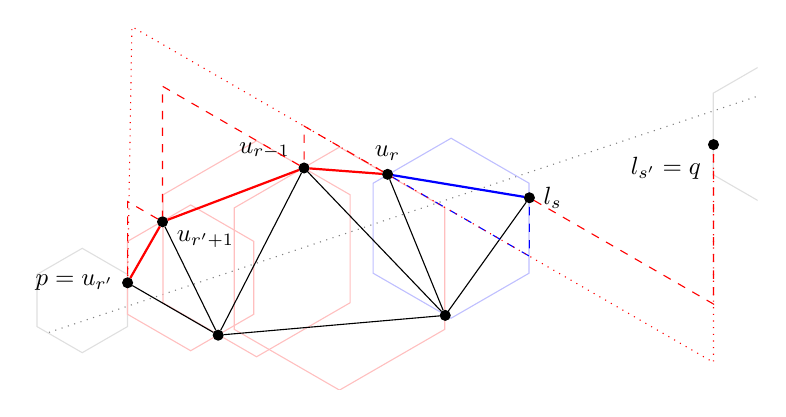
\begin{tikzpicture}[scale=.9, transform shape]
\clip (-0.3,-0.8) rectangle (10,4.3);

\coordinate (t) at (10,3.333);
\coordinate (s) at (0,0);
\draw [gray, dotted] (s) -- (t);



\node [draw, gray!25, shape border rotate=30, minimum size=0.58in, regular polygon, regular polygon sides=6] at (0.47,0.45) (Hm2) {};

\node [color=gray!50, dashed, shape border rotate=30, minimum size=0.78in, regular polygon, regular polygon sides=6] at (1.53,-0.05) (Hm1) {};

\node [draw, color=red!25, shape border rotate=30, minimum size=0.81in, regular polygon, regular polygon sides=6] at (2,0.77) (H0) {};

\node [color=gray!50, shape border rotate=30, minimum size=0.8in, regular polygon, regular polygon sides=6] at (1.73,0.61) (H1) {};

\node [draw, color=red!25, shape border rotate=30, minimum size=1.2in, regular polygon, regular polygon sides=6] at (2.93,1.18) (H2) {};

\node [color=gray!50, shape border rotate=30, minimum size=1.45in, regular polygon, regular polygon sides=6] at (3.99,0.71) (H3) {};

\node [draw, color=red!25, shape border rotate=30, minimum size=1.35in, regular polygon, regular polygon sides=6] at (4.1,0.9) (H4) {};

\node [draw, color=blue!25, shape border rotate=30, minimum size=1in, regular polygon, regular polygon sides=6] at (5.675,1.47) (H5) {};

\node [color=gray!50, shape border rotate=30, minimum size=0.906in, regular polygon, regular polygon sides=6] at (5.775,2.27) (H6) {};

\node [draw, color=gray!25, shape border rotate=30, minimum size=0.906in, regular polygon, regular polygon sides=6] at (10.37,2.8) (H7) {};

%\node at (H0.corner 4) (a) {};
%\node at (H0.corner 5) (b) {};
%\node at (H1.corner 2) (c) {};
%\node at (H1.corner 3) (d) {};

%\node at (intersection of a--b and c--d) [draw,fill,circle,inner sep=1.4pt] (l1) {};

\node at (1.11,0.7) [draw,fill,circle,inner sep=1.4pt,label=180:{$p=u_{r'}$}] (h0) {};

\node at (H1.corner 1) (a) {};
\node at (H1.corner 2) (b) {};
\node at (H2.corner 2) (c) {};
\node at (H2.corner 3) (d) {};

\node at (intersection of a--b and c--d) [draw,fill,circle,inner sep=1.4pt,label=-4:{$u_{r'+1}$}] (h1h2) {};

\node at (H2.corner 3) (a) {};
\node at (H2.corner 4) (b) {};
\node at (H3.corner 2) (c) {};
\node at (H3.corner 3) (d) {};

\node at (intersection of a--b and c--d) [draw,fill,circle,inner sep=1.4pt] (l2l3) {};

\node at (3.6,2.32) [draw,fill,circle,inner sep=1.4pt,label=177:{$u_{r-1}$}] (h3h4) {};

\node at (H4.corner 6) (a) {};
\node at (H4.corner 1) (b) {};
\node at (H5.corner 1) (c) {};
\node at (H5.corner 2) (d) {};

\node at (intersection of a--b and c--d) [draw,fill,circle,inner sep=1.4pt,label=90:{$u_r$}] (h5h6) {};

\node at (6.78,1.9) [draw,fill,circle,inner sep=1.4pt,label=0:{$l_s$}] (l6) {};

\node at (H4.corner 5) (a) {};
\node at (H4.corner 6) (b) {};
\node at (H5.corner 3) (c) {};
\node at (H5.corner 4) (d) {};

\node at (intersection of a--b and c--d) [draw,fill,circle,inner sep=1.4pt] (l4l5) {};

\node (tmp) at ($(h3h4)+(90:4)$) {};
\node (tmp2) at ($(h5h6)+(150:4)$) {};

\coordinate (z3) at (intersection of h3h4--tmp and h5h6--tmp2);

\node (tmp) at ($(h3h4)+(150:4)$) {};
\node (tmp2) at ($(h1h2)+(90:4)$) {};

\coordinate (z2) at (intersection of h3h4--tmp and h1h2--tmp2);

\node (tmp) at ($(h1h2)+(150:4)$) {};
\node (tmp2) at ($(h0)+(90:4)$) {};

\coordinate (z1) at (intersection of h1h2--tmp and h0--tmp2);

\draw [dashed, red] (h5h6) -- (z3) -- (h3h4) -- (z2) -- (h1h2) -- (z1) -- (h0);
%\draw [dashed, red] (h3h4) -- (z2);
%\draw [dashed, red] (h1h2) -- (z1);

\node (tmp) at ($(h5h6)+(150:5)$) {};
\node (tmp2) at ($(h0)+(90:4)$) {};

\coordinate (z) at (intersection of h5h6--tmp and h1h2--tmp2);

\draw [dotted, red] (h5h6) -- (z) -- (h0);


%\node at (H5.corner 5) (a) {};
%\node at (H5.corner 6) (b) {};
%\node at (H6.corner 4) (c) {};
%\node at (H6.corner 5) (d) {};

%\node at (intersection of a--b and c--d) [draw,fill,circle,inner sep=1.4pt,label=270:{$l_5$}] (l5) {};




\draw [thick,red] (h0) -- (h1h2) -- (h3h4) -- (h5h6);
\draw (h0) -- (l2l3);
\draw (h1h2) -- (l2l3) -- (h1h2);
\draw (h3h4) -- (l2l3) -- (l4l5) -- (h3h4);
\draw (h5h6) -- (l4l5) -- (l6);
\draw [thick, blue] (l6) -- (h5h6);
%\draw (h3) -- (l4) -- (h1);


\coordinate (tmp) at ($(h5h6)+(-30:8)$);
\coordinate (tmp2) at ($(l6)+(-90:6)$);

\coordinate (z4) at (intersection of h5h6--tmp and l6--tmp2);

\draw [dashed, blue] (h5h6) -- (z4) -- (l6);

\coordinate (tmp) at ($(l6)+(-30:3)$);
\node at ($(tmp)+(90:2.25)$) [draw,fill,circle,inner sep=1.4pt,label=-135:{$l_{s'}=q$}] (tmp2) {};


\coordinate (tmp3) at ($(z4)+(-30:6)$);
\coordinate (tmp4) at ($(tmp)+(-90:4)$);

\coordinate (z5) at (intersection of z4--tmp3 and tmp--tmp4);

\draw [dotted, red] (h5h6) -- (z5) -- (tmp2);

\draw [dashed, red] (l6) -- (tmp) -- (tmp2);
\end{tikzpicture}
}





\def\tikzbox{
\clip (-0.42,-1.5) rectangle (4.05,3);
%\node at (0,0)  (s) [draw,fill,circle,inner sep=2pt,label=180:{$s$}] {};
\coordinate (t) at (4,2.5);
\coordinate (s) at (-.5,0);
%\node [draw, color=gray, shape border rotate=30, minimum size=1in, regular polygon, regular polygon sides=6] at (1.1,0) (H1) {};


%\draw [shift=(H1.side 2)] plot[mark=*,mark size=1.9pt] coordinates{(0,0)} 
%node [left] (s) {{$s$}};

%\node [draw, color=gray, dashed, shape border rotate=30, minimum size=1.3in, regular polygon, regular polygon sides=6] at (1.8,.5) (H2) {};

%\node at (H1.corner 1) (a) {};
%\node at (H1.corner 2) (b) {};
%\node at (H2.corner 2) (c) {};
%\node at (H2.corner 3) (d) {};

%\node at (intersection of a--b and c--d) [draw,fill,circle,inner sep=1.4pt,label=175:{$u_1$}] (h1) {};

\node [transform shape,draw, color=red!25, shape border rotate=30, minimum size=0.7in, regular polygon, regular polygon sides=6] at (0.51,1.2) (H0) {};

%\node at (H0.side 3) [draw, circle, fill, inner sep=1.4pt,label=180:$s$] {};

\node at (0.16,0.51) [transform shape,inner sep=1.4pt, draw,circle,fill=red,label=180:{$u_r$}] (h0) {};

\draw [gray, dotted] (s) -- (t);


\node [transform shape,draw, color=blue!25, shape border rotate=30, minimum size=0.8in, regular polygon, regular polygon sides=6] at (.87,1.35) (H1) {};

\node [draw, color=red!25, shape border rotate=30, minimum size=0.95in, regular polygon, regular polygon sides=6] at (1.2,1.35) (H2) {};

\node [draw, color=blue!25, shape border rotate=30, minimum size=0.95in, regular polygon, regular polygon sides=6] at (1.3,1.41) (H3) {};

\node [draw, color=red!25, shape border rotate=30, minimum size=0.75in, regular polygon, regular polygon sides=6] at (1.74,1.41) (H4) {};

\node [draw, color=blue!25, shape border rotate=30, minimum size=0.685in, regular polygon, regular polygon sides=6] at (1.96,1.53) (H5) {};

\node [draw, color=red!25, shape border rotate=30, minimum size=0.6in, regular polygon, regular polygon sides=6] at (2.9,1.59) (H6) {};

%\node [draw, color=gray!50, shape border rotate=30, minimum size=0.906in, regular polygon, regular polygon sides=6] at (10.37,2.8) (H7) {};

\node at (H0.corner 4) (a) {};
\node at (H0.corner 5) (b) {};
\node at (H1.corner 3) (c) {};
\node at (H1.corner 4) (d) {};

\node at (intersection of a--b and c--d) [transform shape,draw,fill,circle,inner sep=1.4pt,label=270:{$l_{r+1}$}] (l1) {};

\node at (H0.corner 1) (az) {};
\node at (H0.corner 2) (bz) {};
\node at (H1.corner 2) (cz) {};
\node at (H1.corner 3) (dz) {};

\node at (intersection of az--bz and cz--dz) [transform shape,draw,fill,circle,inner sep=1.4pt] (h1) {};


\node at (.47,2.14) [draw,fill,circle,inner sep=1.4pt] (h2) {};

\node at (2.02,0.62) [draw,fill,circle,inner sep=1.4pt] (l2) {};

\node at (1.82,2.32) [draw,fill,circle,inner sep=1.4pt] (h3) {};

\node at (2.57,1.02) [draw,fill,circle,inner sep=1.4pt] (l3) {};

\node at (2.47,2.1) [transform shape,draw,fill,circle,inner sep=1.4pt,label=90:{$u_{s-1}$}] (h4) {};

\node at (3.45,2.03) [transform shape,draw,fill=red,circle,inner sep=1.4pt,label=0:{$l_s$}] (l4) {};


%\node at (H1.corner 1) (a) {};
%\node at (H1.corner 2) (b) {};
%\node at (H2.corner 2) (c) {};
%\node at (H2.corner 3) (d) {};

%\node at (intersection of a--b and c--d) [draw,fill,circle,inner sep=1.4pt,label=180:{$u_{r'}$}] (h1h2) {};

%\node at (H2.corner 3) (a) {};
%\node at (H2.corner 4) (b) {};
%\node at (H3.corner 2) (c) {};
%\node at (H3.corner 3) (d) {};

%\node at (intersection of a--b and c--d) [draw,fill,circle,inner sep=1.4pt] (l2l3) {};


%\node at (H4.corner 6) (a) {};
%\node at (H4.corner 1) (b) {};
%\node at (H5.corner 1) (c) {};
%\node at (H5.corner 2) (d) {};

%\node at (intersection of a--b and c--d) [draw,fill,circle,inner sep=1.4pt,label=45:{$u_r$}] (h5h6) {};

%\node at (6.78,1.9) [draw,fill,circle,inner sep=1.4pt,label=45:{$l_s$}] (l6) {};

%\node at (H4.corner 5) (a) {};
%\node at (H4.corner 6) (b) {};
%\node at (H5.corner 3) (c) {};
%\node at (H5.corner 4) (d) {};

%\node at (intersection of a--b and c--d) [draw,fill,circle,inner sep=1.4pt] (l4l5) {};

%\node (tmp) at ($(h0)+(90:10)$) [transform shape] {};
%\node (tmp2) at ($(l4)+(150:10)$) [transform shape] {};

%\coordinate (z) at (intersection of h0--tmp and l4--tmp2);
\coordinate (z) at (3.45, -1.39);

%\node (tmp) at ($(h3h4)+(150:4)$) {};
%\node (tmp2) at ($(h1h2)+(90:4)$) {};

%\coordinate (z2) at (intersection of h3h4--tmp and h1h2--tmp2);

\draw [transform shape, dashed, red] (h0) -- (z);
\draw [transform shape, dashed, red] (l4) -- (z);

%\node (tmp) at ($(h5h6)+(150:4)$) {};
%\node (tmp2) at ($(h1h2)+(90:3)$) {};

%\coordinate (z3) at (intersection of h5h6--tmp and h1h2--tmp2);

%\draw [dashed, red] (h5h6) -- (z3) -- (h1h2);

%\draw [thick,red] (h1h2) -- (h3h4) -- (h5h6);

%\draw (h1h2) -- (l1) -- (l2l3) -- (h1h2);
%\draw (h3h4) -- (l2l3) -- (l4l5) -- (h3h4);
%\draw (h5h6) -- (l4l5) -- (l6);
%\draw [thick, blue] (l6) -- (h5h6);
%\draw (h3) -- (l4) -- (h1);

\draw [blue,thick] (l1) -- (h0);
\draw (h0) -- (h1) -- (l1) -- (h2) -- (h1);
\draw (l1) -- (l2) -- (h2) -- (h3) -- (l2) -- (l3) -- (h3) -- (h4) -- (l3) -- (l4) -- (h4);

%\coordinate (z4) at (0,-0.5);

%\draw (t) -- (s) -- (z4);
%pic [draw=green!50!black, fill=green!20, angle radius=9mm,
%             "$\alpha$"] {angle = t--s--z4};

%\coordinate (tmp) at ($(h5h6)+(-30:8)$);
%\coordinate (tmp2) at ($(l6)+(-90:6)$);

%\coordinate (z4) at (intersection of h5h6--tmp and l6--tmp2);

%\draw [dashed, blue] (h5h6) -- (z4) -- (l6);

%\coordinate (tmp) at ($(l6)+(-30:3)$);
%\node at ($(tmp)+(90:2.25)$) [draw,fill,circle,inner sep=1.4pt,label=180:{$l_{s'}$}] (tmp2) {};

%\draw [dashed, red] (l6) -- (tmp) -- (tmp2);
}


\newcommand{\caseB}{
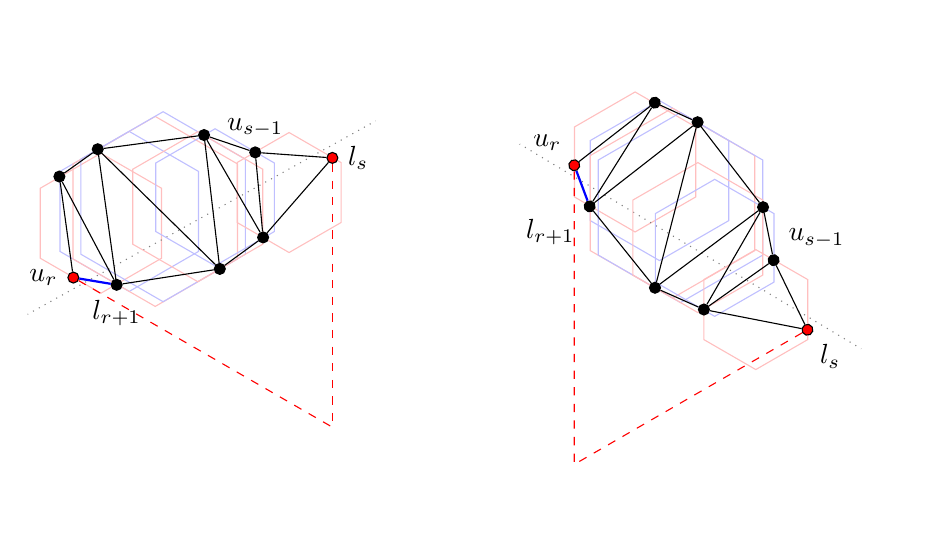
\begin{tikzpicture}
\begin{scope}
\tikzbox
\end{scope}
%\begin{scope}[shift={(6,-0.8)},yscale=-1,xscale=1,rotate=-60]
\begin{scope}[shift={(6,1.82)},yscale=1,xscale=1,rotate=-60]
\tikzbox
\end{scope}
\end{tikzpicture}
}


\newcommand{\othercase}{
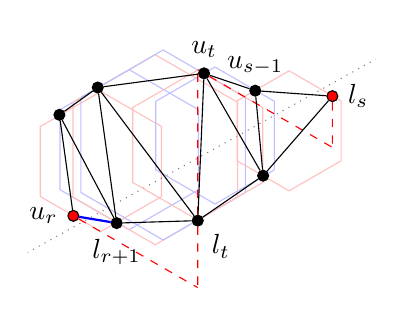
\begin{tikzpicture}[scale=1, transform shape]
\clip (-0.42,-0.5) rectangle (4.05,2.9);
%\node at (0,0)  (s) [draw,fill,circle,inner sep=2pt,label=180:{$s$}] {};
\coordinate (t) at (4,2.5);
\coordinate (s) at (-.5,0);
%\node [draw, color=gray, shape border rotate=30, minimum size=1in, regular polygon, regular polygon sides=6] at (1.1,0) (H1) {};


%\draw [shift=(H1.side 2)] plot[mark=*,mark size=1.9pt] coordinates{(0,0)} 
%node [left] (s) {{$s$}};

%\node [draw, color=gray, dashed, shape border rotate=30, minimum size=1.3in, regular polygon, regular polygon sides=6] at (1.8,.5) (H2) {};

%\node at (H1.corner 1) (a) {};
%\node at (H1.corner 2) (b) {};
%\node at (H2.corner 2) (c) {};
%\node at (H2.corner 3) (d) {};

%\node at (intersection of a--b and c--d) [draw,fill,circle,inner sep=1.4pt,label=175:{$u_1$}] (h1) {};

\node [transform shape,draw, color=red!25, shape border rotate=30, minimum size=0.7in, regular polygon, regular polygon sides=6] at (0.51,1.2) (H0) {};

%\node at (H0.side 3) [draw, circle, fill, inner sep=1.4pt,label=180:$s$] {};

\node at (0.16,0.51) [transform shape,inner sep=1.4pt, draw,circle,fill=red,label=180:{$u_r$}] (h0) {};

\draw [gray, dotted] (s) -- (t);


\node [transform shape,draw, color=blue!25, shape border rotate=30, minimum size=0.8in, regular polygon, regular polygon sides=6] at (.87,1.35) (H1) {};

\node [draw, color=red!25, shape border rotate=30, minimum size=0.95in, regular polygon, regular polygon sides=6] at (1.2,1.35) (H2) {};

\node [draw, color=blue!25, shape border rotate=30, minimum size=0.95in, regular polygon, regular polygon sides=6] at (1.3,1.41) (H3) {};

\node [draw, color=red!25, shape border rotate=30, minimum size=0.75in, regular polygon, regular polygon sides=6] at (1.74,1.41) (H4) {};

\node [draw, color=blue!25, shape border rotate=30, minimum size=0.685in, regular polygon, regular polygon sides=6] at (1.96,1.53) (H5) {};

\node [draw, color=red!25, shape border rotate=30, minimum size=0.6in, regular polygon, regular polygon sides=6] at (2.9,1.59) (H6) {};

%\node [draw, color=gray!50, shape border rotate=30, minimum size=0.906in, regular polygon, regular polygon sides=6] at (10.37,2.8) (H7) {};

\node at (H0.corner 4) (a) {};
\node at (H0.corner 5) (b) {};
\node at (H1.corner 3) (c) {};
\node at (H1.corner 4) (d) {};

\node at (intersection of a--b and c--d) [transform shape,draw,fill,circle,inner sep=1.4pt,label=270:{$l_{r+1}$}] (l1) {};

\node at (H0.corner 1) (az) {};
\node at (H0.corner 2) (bz) {};
\node at (H1.corner 2) (cz) {};
\node at (H1.corner 3) (dz) {};

\node at (intersection of az--bz and cz--dz) [transform shape,draw,fill,circle,inner sep=1.4pt] (h1) {};


\node at (.47,2.14) [draw,fill,circle,inner sep=1.4pt] (h2) {};

\node at (H4.corner 4) [draw,fill,circle,inner sep=1.4pt,label=-45:{$l_{t}$}] (l2) {};

\node at (1.82,2.32) [draw,fill,circle,inner sep=1.4pt,label=90:{$u_{t}$}] (h3) {};

\node at (2.57,1.02) [draw,fill,circle,inner sep=1.4pt] (l3) {};

\node at (2.47,2.1) [transform shape,draw,fill,circle,inner sep=1.4pt,label=90:{$u_{s-1}$}] (h4) {};

\node at (3.45,2.03) [transform shape,draw,fill=red,circle,inner sep=1.4pt,label=0:{$l_s$}] (l4) {};


\node (tmp) at ($(h0)+(-30:10)$) [transform shape] {};
\node (tmp2) at ($(l2)+(-90:10)$) [transform shape] {};

\coordinate (z) at (intersection of h0--tmp and l2--tmp2);

\draw [transform shape, dashed, red] (h0) -- (z);
\draw [transform shape, dashed, red] (l2) -- (z);


\node (tmp) at ($(l2)+(90:10)$) [transform shape] {};
\node (tmp2) at ($(h3)+(150:10)$) [transform shape] {};

\coordinate (z) at (intersection of l2--tmp and h3--tmp2);

\draw [transform shape, dashed, red] (l2) -- (z);
\draw [transform shape, dashed, red] (h3) -- (z);


\node (tmp) at ($(h3)+(-30:10)$) [transform shape] {};
\node (tmp2) at ($(l4)+(-90:10)$) [transform shape] {};

\coordinate (z) at (intersection of h3--tmp and l4--tmp2);

\draw [transform shape, dashed, red] (h3) -- (z);
\draw [transform shape, dashed, red] (l4) -- (z);




%\coordinate (z) at (3.45, -1.39);




%\node (tmp) at ($(h3h4)+(150:4)$) {};
%\node (tmp2) at ($(h1h2)+(90:4)$) {};

%\coordinate (z2) at (intersection of h3h4--tmp and h1h2--tmp2);


%\node (tmp) at ($(h5h6)+(150:4)$) {};
%\node (tmp2) at ($(h1h2)+(90:3)$) {};

%\coordinate (z3) at (intersection of h5h6--tmp and h1h2--tmp2);

%\draw [dashed, red] (h5h6) -- (z3) -- (h1h2);

%\draw [thick,red] (h1h2) -- (h3h4) -- (h5h6);

%\draw (h1h2) -- (l1) -- (l2l3) -- (h1h2);
%\draw (h3h4) -- (l2l3) -- (l4l5) -- (h3h4);
%\draw (h5h6) -- (l4l5) -- (l6);
%\draw [thick, blue] (l6) -- (h5h6);
%\draw (h3) -- (l4) -- (h1);

\draw [blue,thick] (l1) -- (h0);
\draw (h0) -- (h1) -- (l1) -- (h2) -- (h1);
\draw (l1) -- (l2) -- (h2) -- (h3) -- (l2) -- (l3) -- (h3) -- (h4) -- (l3) -- (l4) -- (h4);
\end{tikzpicture}
}



\newcommand{\notation}{
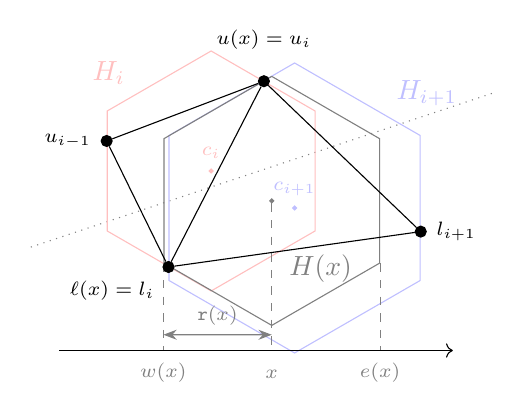
\begin{tikzpicture}[scale=1, transform shape]
\clip (0.6,-1.55) rectangle (6.5,3);

\coordinate (t) at (10,3.333);
\coordinate (s) at (0,0);
\draw [gray, dotted] (s) -- (t);

\node [color=gray!50, shape border rotate=30, minimum size=0.8in, regular polygon, regular polygon sides=6] at (1.73,0.61) (H1) {};

\node [draw, color=red!25, shape border rotate=30, minimum size=1.2in, regular polygon, regular polygon sides=6,label=135:{\color{red!25}{$H_i$}}] at (2.93,1.18) (H2) {};

\node [draw,circle,fill,color=red!25,inner sep=0.5pt,label=90:{\scriptsize\color{red!25}{$c_i$}}] at (2.93,1.18) {};

\node [draw, color=blue!25, shape border rotate=30, minimum size=1.45in, regular polygon, regular polygon sides=6,label=45:{\color{blue!25}{$H_{i+1}$}}] at (3.99,0.71) (H3) {};

\node [draw,circle,fill,color=blue!25,inner sep=0.5pt,label=90:{\scriptsize\color{blue!25}{$c_{i+1}$}}] at (3.99,0.71) {};

\node [draw, color=gray, shape border rotate=30, minimum size=1.245in, regular polygon, regular polygon sides=6,label={[label distance=-0.9cm]-80:{\color{gray}{$H(x)$}}}] at (3.7,0.8) (H25) {};

\node [color=red!25, shape border rotate=30, minimum size=1.35in, regular polygon, regular polygon sides=6] at (4.1,0.9) (H4) {};


\node [draw,circle,fill,color=gray,inner sep=0.5pt] at (3.7,0.8) (c) {};


\coordinate (cx) at (3.7,-1.1);
\draw [dashed,gray] (c) -- (cx); 
\node at (cx) [label={[gray]-90:{{\scriptsize $x$}}}] {};

\coordinate (wx) at ($(H25.corner 3) + (0,-1.105)$);
\draw [dashed,gray] (H25.corner 3) -- (wx); 
\node at (wx) [label={[label distance=-0.089cm,gray]-90:{{\scriptsize $w(x)$}}}] {};

\coordinate (ex) at ($(H25.corner 5) + (0,-1.105)$);
\draw [dashed,gray] (H25.corner 5) -- (ex); 
\node at (ex) [label={[label distance=-0.089cm,gray]-90:{{\scriptsize $e(x)$}}}] {};

\draw [gray,<->,{Stealth-Stealth},label=90:${\tt r}(x)$] ($(cx)+(0,0.2)$) -- ($(wx)+(0,0.2)$) node [midway, above] {\scriptsize ${\tt r}(x)$};
\draw [->] (1,-1.1) -- (6,-1.1);





\node at (H1.corner 1) (a) {};
\node at (H1.corner 2) (b) {};
\node at (H2.corner 2) (c) {};
\node at (H2.corner 3) (d) {};

\node at (intersection of a--b and c--d) [draw,fill,circle,inner sep=1.4pt,label=180:{\scriptsize $u_{i-1}$}] (h1h2) {};

\node at (H2.corner 3) (a) {};
\node at (H2.corner 4) (b) {};
\node at (H3.corner 2) (c) {};
\node at (H3.corner 3) (d) {};

\node at (intersection of a--b and c--d) [draw,fill,circle,inner sep=1.4pt,label=-135:{\scriptsize $\ell(x)=l_i$}] (l2l3) {};

\node at (3.6,2.32) [draw,fill,circle,inner sep=1.4pt,label={[label distance=0.2cm]90:{\scriptsize $u(x)=u_i$}}] (h3h4) {};

%\node at (H4.corner 5) (a) {};
%\node at (H4.corner 6) (b) {};
%\node at (H5.corner 3) (c) {};
%\node at (H5.corner 4) (d) {};

%\node at (intersection of a--b and c--d) [draw,fill,circle,inner sep=1.4pt,label=0:{\scriptsize $l_{i+1}$}] (l4l5) {};

\node at (H3.side 5) [draw,yshift=-.3cm,fill,circle,inner sep=1.4pt,label=0:{\scriptsize $l_{i+1}$}] (l4l5) {};

\draw (l2l3) -- (h1h2) -- (h3h4) -- (l4l5) -- (l2l3) -- (h3h4);
\end{tikzpicture}
}




\newcommand{\dNdS}{
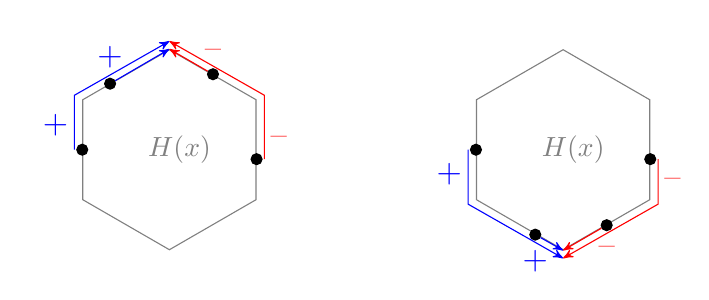
\begin{tikzpicture}[scale=1]
\clip (-1.8,-1.55) rectangle (6.5,1.55);
\node (h) [draw, color=gray, shape border rotate=30, minimum size=1in, regular polygon, regular polygon sides=6,label={[label distance=-1.5cm]0:{\color{gray}{$H(x)$}}}] at (0,0) {};

\node at (h.side 1) [xshift=-0.2cm,yshift=-0.12cm,draw,circle,fill,inner sep=1.4pt,label=90:{\color{blue}{\large +}}] (s1) {};
\node at (h.side 2) [draw,circle,fill,inner sep=1.4pt,label=135:{\color{blue}{\large +}}] (s2) {};
%\node at (h.side 3) [xshift=+0.2cm,yshift=-0.12cm,draw,circle,fill,inner sep=1.4pt,label=90:{\color{blue}{\large +}}] (s3) {};

\draw (s1) -- (h.corner 1) [->,>=stealth',blue,label=-45:{$+$}];
\draw ($(s2) + (-0.1cm,0)$) -- ($(h.corner 2) + (-0.1cm,0.052cm)$) -- ($(h.corner 1) + (0,0.1cm)$) [->,>=stealth',blue,label=-45:{$+$}];
%\draw ($(s3) + (0.052cm,0.1cm)$) -- ($(h.corner 3) + (0.1cm,0.052cm)$) -- ($(h.corner 2) + (0.1cm,-0.052cm)$) -- ($(h.corner 1) + (0,-0.1cm)$) [->,>=stealth',blue,label=-45:{$+$}];

\node at (h.side 6) [draw,circle,fill,inner sep=1.4pt,label=90:{\color{red}{\large --}}] (s1) {};
\node at (h.side 5) [yshift=-0.12cm,draw,circle,fill,inner sep=1.4pt,label=45:{\color{red}{\large --}}] (s2) {};
%\node at (h.side 4) [draw,circle,fill,inner sep=1.4pt,label=90:{\color{red}{\large --}}] (s3) {};

\draw (s1) -- (h.corner 1) [->,>=stealth',red];
\draw ($(s2) + (0.1cm,0)$) -- ($(h.corner 6) + (0.1cm,0.052cm)$) -- ($(h.corner 1) + (0,0.1cm)$) [->,>=stealth',red];
%\draw ($(s3) + (-0.052,0.1cm)$) -- ($(h.corner 5) + (-0.1cm,0.052cm)$) -- ($(h.corner 6) + (-0.1cm,-0.052cm)$) -- ($(h.corner 1) + (0,-0.1cm)$) [->,>=stealth',red];

\node (h) [draw, color=gray, shape border rotate=30, minimum size=1in, regular polygon, regular polygon sides=6,label={[label distance=-1.5cm]0:{\color{gray}{$H(x)$}}}] at (5,0) {};

%\node at (h.side 1) [xshift=-0.2cm,yshift=-0.12cm,draw,circle,fill,inner sep=1.4pt,label=-90:{\color{blue}{\large +}}] (s1) {};
\node at (h.side 2) [draw,circle,fill,inner sep=1.4pt,label=-135:{\color{blue}{\large +}}] (s2) {};
\node at (h.side 3) [xshift=+0.2cm,yshift=-0.12cm,draw,circle,fill,inner sep=1.4pt,label=-90:{\color{blue}{\large +}}] (s3) {};

\draw (s3) -- (h.corner 4) [->,>=stealth',blue,label=-45:{$+$}];
\draw ($(s2) + (-0.1cm,0)$) -- ($(h.corner 3) + (-0.1cm,-0.052cm)$) -- ($(h.corner 4) + (0,-0.1cm)$) [->,>=stealth',blue,label=-45:{$+$}];
%\draw ($(s1) + (0.052cm,-0.09cm)$) -- ($(h.corner 2) + (0.1cm,-0.052cm)$) -- ($(h.corner 3) + (0.1cm,0.052cm)$) -- ($(h.corner 4) + (0,0.1cm)$) [->,>=stealth',blue,label=-45:{$+$}];

%\node at (h.side 6) [draw,circle,fill,inner sep=1.4pt,label=-90:{\color{red}{\large --}}] (s1) {};
\node at (h.side 5) [yshift=-0.12cm,draw,circle,fill,inner sep=1.4pt,label=-45:{\color{red}{\large --}}] (s2) {};
\node at (h.side 4) [draw,circle,fill,inner sep=1.4pt,label=-90:{\color{red}{\large --}}] (s3) {};

\draw (s3) -- (h.corner 4) [->,>=stealth',red];
\draw ($(s2) + (0.1cm,0)$) -- ($(h.corner 5) + (0.1cm,-0.052cm)$) -- ($(h.corner 4) + (0,-0.1cm)$) [->,>=stealth',red];
%\draw ($(s1) + (-0.052,-0.1cm)$) -- ($(h.corner 6) + (-0.1cm,-0.052cm)$) -- ($(h.corner 5) + (-0.1cm,0.052cm)$) -- ($(h.corner 4) + (0,0.1cm)$) [->,>=stealth',red];
\end{tikzpicture}\hspace{1.34cm}
\begin{tikzpicture}[scale=1]
\clip (-2.35,-1.45) rectangle (6.5,1.65);
\node (h) [draw, color=gray, shape border rotate=30, minimum size=1in, regular polygon, regular polygon sides=6,label={[label distance=-2cm]0:{\color{gray}{$H(x)=H_i$}}}] at (0,0) {};

\node at (h.side 2) [draw,circle,fill,inner sep=1.4pt,label=180:{$u_{i-1}$}] (uj) {};
\node at (h.side 6) [draw,circle,fill,inner sep=1.4pt,label=0:{$u_i$}] (ujp) {};

\draw (uj) -- (h.corner 2) -- (h.corner 1) [->,>=stealth',blue];
\draw (ujp) -- (h.corner 1) [->,>=stealth',red];

\draw (uj) -- (ujp);

\node at (-1.45,1.1) [blue] {$p_N(u_{i-1},x)$};
\node at (1.05,1.45) [red] {$p_N(u_i,x)$};
\end{tikzpicture}
}


\newcommand{\UandL}{
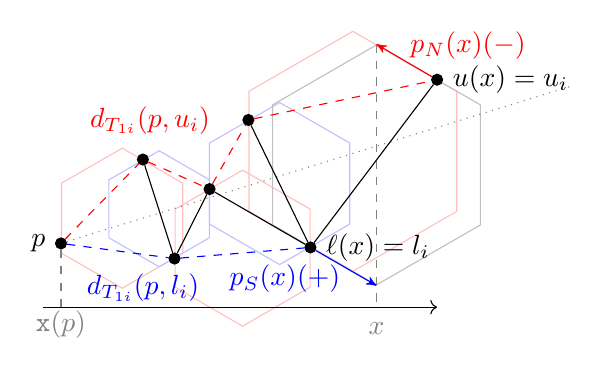
\begin{tikzpicture}[scale=1, transform shape]
\clip (-1.2,-1.3) rectangle (5.7,2.75);


\node [draw, color=red!25, shape border rotate=30, minimum size=0.7in, regular polygon, regular polygon sides=6] at (0,0.33) (Hm3) {};

\node [draw, color=blue!25, shape border rotate=30, minimum size=0.58in, regular polygon, regular polygon sides=6] at (0.47,0.45) (Hm2) {};

\node [draw,color=red!25, shape border rotate=30, minimum size=0.78in, regular polygon, regular polygon sides=6] at (1.53,-0.05) (Hm1) {};

\node [draw, color=blue!25, shape border rotate=30, minimum size=0.81in, regular polygon, regular polygon sides=6] at (2,0.77) (H1) {};

\node [draw, color=red!25, shape border rotate=30, minimum size=1.2in, regular polygon, regular polygon sides=6] at (2.93,1.18) (H2) {};

\node [draw, color=gray!50, shape border rotate=30, minimum size=1.2in, regular polygon, regular polygon sides=6] at ($(2.93,1.18)+ (1*0.3, -.577*0.3)$) (H3) {};

\node at (Hm3.side 2) [yshift=-0.32cm,draw,circle,fill,inner sep=1.4pt,label=180:{$p$}] (s) {};

\node at (10,3.333) [draw,fill,circle,inner sep=1.4pt,label=180:{$t$}] (t) {};

\draw [gray, dotted] (s) -- (t);

\coordinate (o) at (-1,-.8);
\coordinate (x) at (4,-.8);
\draw [->] (o) -- (x);

\coordinate (N) at (H3.corner 1);
\draw [gray, dashed] (N) -- (N |- 52,-.8);
\node at (N |- 52,-.8) [label={[label distance=-0.05cm]-90:{\color{gray}{$x$}}}] {};
\draw [gray, dashed] (s) -- (s |- 52,-.8);
\node at (s |- 52,-.8) [label={[label distance=-0.2cm]-90:{\color{gray}{${\tt x}(p)$}}}] {};


%\draw (ul) -- (l);




\node at (Hm3.corner 6) (a) {};
\node at (Hm3.corner 1) (b) {};
\node at (Hm2.corner 1) (c) {};
\node at (Hm2.corner 2) (d) {};

\node at (intersection of a--b and c--d) [draw,fill,circle,inner sep=1.4pt] (h1) {};

\node at (Hm2.corner 4) (a) {};
\node at (Hm2.corner 5) (b) {};
\node at (Hm1.corner 2) (c) {};
\node at (Hm1.corner 3) (d) {};

\node at (intersection of a--b and c--d) [draw,fill,circle,inner sep=1.4pt] (l1) {};

\node at (1.11,0.7) [draw,fill,circle,inner sep=1.4pt] (h2) {};

\node at (H1.corner 1) (a) {};
\node at (H1.corner 2) (b) {};
\node at (H2.corner 2) (c) {};
\node at (H2.corner 3) (d) {};

\node at (intersection of a--b and c--d) [draw,fill,circle,inner sep=1.4pt] (h4) {};

\node at (H2.corner 3) (a) {};
\node at (H2.corner 4) (b) {};
\node at (H1.corner 4) (c) {};
\node at (H1.corner 5) (d) {};

\node at (intersection of a--b and c--d) [draw,fill,circle,inner sep=1.4pt,label=0:{$\ell(x)=l_i$}] (l3) {};

\node at ($(3.6,2.32) + (1*0.4, -.577*0.4)$) [draw, fill,circle,inner sep=1.4pt,label=0:{$u(x)=u_i$}] (h5) {};




\draw (h1) -- (l1) -- (h2) -- (l3) -- (h4);
\draw (l3) -- (h5);
\draw [red,dashed] (s) -- (h1) -- (h2) -- (h4) -- (h5);
\draw [blue,dashed] (s) -- (l1) -- (l3);

\node at (H2.corner 2) [red,xshift=-1.25cm,yshift=-0.37cm] {$d_{T_{1i}}(p,u_i)$};
\node at (Hm1.corner 3) [blue,xshift=-.4cm,yshift=0cm] {$d_{T_{1i}}(p,l_i)$};


\draw (h5) -- (H3.corner 1) [->,>=stealth',red];
\node at (H3.side 6) [red,xshift=0.5cm,yshift=0.37cm] {$p_N(x) (-)$};

\draw (l3) -- (H3.corner 4) [->,>=stealth',blue];
\node at (H3.side 3) [blue,xshift=-0.5cm,yshift=-0.3cm] {$p_S(x) (+)$};


\end{tikzpicture}\hspace{-0.2cm}
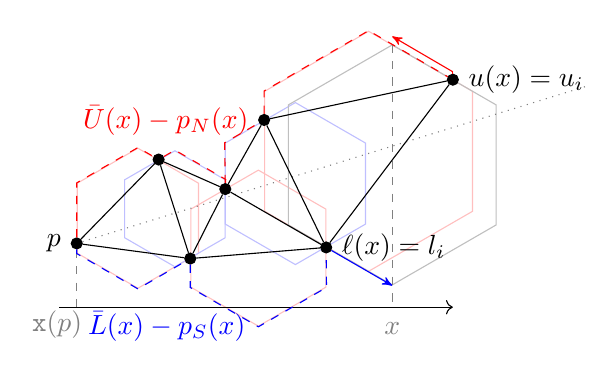
\begin{tikzpicture}[scale=1, transform shape]
\clip (-1.4,-1.3) rectangle (5.7,2.75);


\node [draw, color=red!25, shape border rotate=30, minimum size=0.7in, regular polygon, regular polygon sides=6] at (0,0.33) (Hm3) {};

\node [draw, color=blue!25, shape border rotate=30, minimum size=0.58in, regular polygon, regular polygon sides=6] at (0.47,0.45) (Hm2) {};

\node [draw,color=red!25, shape border rotate=30, minimum size=0.78in, regular polygon, regular polygon sides=6] at (1.53,-0.05) (Hm1) {};

\node [draw, color=blue!25, shape border rotate=30, minimum size=0.81in, regular polygon, regular polygon sides=6] at (2,0.77) (H1) {};

\node [draw, color=red!25, shape border rotate=30, minimum size=1.2in, regular polygon, regular polygon sides=6] at (2.93,1.18) (H2) {};

\node [draw, color=gray!50, shape border rotate=30, minimum size=1.2in, regular polygon, regular polygon sides=6] at ($(2.93,1.18)+ (1*0.3, -.577*0.3)$) (H3) {};

\node at (Hm3.side 2) [yshift=-0.32cm,draw,circle,fill,inner sep=1.4pt,label=180:{$p$}] (s) {};

\node at (10,3.333) [draw,fill,circle,inner sep=1.4pt,label=180:{$t$}] (t) {};

\draw [gray, dotted] (s) -- (t);

\coordinate (o) at (-1,-.8);
\coordinate (x) at (4,-.8);
\draw [->] (o) -- (x);

\coordinate (N) at (H3.corner 1);
\draw [gray, dashed] (N) -- (N |- 52,-.8);
\node at (N |- 52,-.8) [label={[label distance=-0.05cm]-90:{\color{gray}{$x$}}}] {};
\draw [gray, dashed] (s) -- (s |- 52,-.8);
\node at ($(s |- 52,-.8) + (-0.25,0)$) [label={[label distance=-0.2cm]-90:{\color{gray}{${\tt x}(p)$}}}] {};


%\draw (ul) -- (l);




\node at (Hm3.corner 6) (a) {};
\node at (Hm3.corner 1) (b) {};
\node at (Hm2.corner 1) (c) {};
\node at (Hm2.corner 2) (d) {};

\node at (intersection of a--b and c--d) [draw,fill,circle,inner sep=1.4pt] (h1) {};

\node at (Hm2.corner 4) (a) {};
\node at (Hm2.corner 5) (b) {};
\node at (Hm1.corner 2) (c) {};
\node at (Hm1.corner 3) (d) {};

\node at (intersection of a--b and c--d) [draw,fill,circle,inner sep=1.4pt] (l1) {};

\node at (1.11,0.7) [draw,fill,circle,inner sep=1.4pt] (h2) {};

\node at (H1.corner 1) (a) {};
\node at (H1.corner 2) (b) {};
\node at (H2.corner 2) (c) {};
\node at (H2.corner 3) (d) {};

\node at (intersection of a--b and c--d) [draw,fill,circle,inner sep=1.4pt] (h4) {};

\node at (H2.corner 3) (a) {};
\node at (H2.corner 4) (b) {};
\node at (H1.corner 4) (c) {};
\node at (H1.corner 5) (d) {};

\node at (intersection of a--b and c--d) [draw,fill,circle,inner sep=1.4pt,label=0:{$\ell(x)=l_i$}] (l3) {};

\node at ($(3.6,2.32) + (1*0.4, -.577*0.4)$) [draw, fill,circle,inner sep=1.4pt,label=0:{$u(x)=u_i$}] (h5) {};




\draw (h1) -- (l1) -- (h2) -- (l3) -- (h4);
\draw (l3) -- (h5);
\draw (s) -- (h1) -- (h2) -- (h4) -- (h5);
\draw (s) -- (l1) -- (l3);

\draw [red,dashed] (s) -- (Hm3.corner 2) -- (Hm3.corner 1) -- (h1) -- (Hm2.corner 1) --(Hm2.corner 6) -- (h2) -- (H1.corner 2) -- (h4) -- (H2.corner 2) -- (H2.corner 1) -- (h5);  

\draw [red] (h5) --  ($(h5) + (0, 0.1cm)$);
\draw ($(h5) + (0, 0.1cm)$) -- ($(H3.corner 1) + (0, 0.1cm)$) [->,>=stealth',red];
%\node at (H3.side 6) [red,xshift=0.64cm,yshift=0.4cm] {$p_N(x) (-)$};

\draw [blue,dashed] (s) -- (Hm3.corner 3) -- (Hm3.corner 4) -- (l1) -- (Hm1.corner 3) --(Hm1.corner 4) -- (Hm1.corner 5) -- (l3);  

\draw (l3) -- (H3.corner 4) [->,>=stealth',blue];
%\node at (H3.side 3) [blue,xshift=-0.5cm,yshift=-0.37cm] {$p_S(x) (+)$};


\node at (H2.corner 2) [red,xshift=-1.25cm,yshift=-0.37cm] {$\bar{U}(x)-p_N(x)$};
\node at (Hm1.corner 3) [blue,xshift=-.3cm,yshift=-0.5cm] {$\bar{L}(x)-p_S(x)$};

\end{tikzpicture}
}





\newcommand{\transitiononezero}{
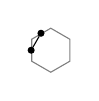
\begin{tikzpicture}[scale=1]
\node (h) [draw, color=gray, shape border rotate=30, minimum size=0.22in, regular polygon, regular polygon sides=6] at (0,0) {};
\node at (h.side 2) [draw,circle,fill,inner sep=0.75pt] (s1) {};
\node at (h.side 1) [draw,circle,fill,inner sep=0.75pt] (s2) {};
\draw (s1)--(s2);
\end{tikzpicture}
}

\newcommand{\transitiononefive}{
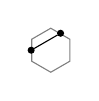
\begin{tikzpicture}[scale=1]
\node (h) [draw, color=gray, shape border rotate=30, minimum size=0.22in, regular polygon, regular polygon sides=6] at (0,0) {};
\node at (h.side 2) [draw,circle,fill,inner sep=0.75pt] (s1) {};
\node at (h.side 6) [draw,circle,fill,inner sep=0.75pt] (s2) {};
\draw (s1)--(s2);
\end{tikzpicture}
}

\newcommand{\transitiontwoone}{
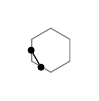
\begin{tikzpicture}[scale=1]
\node (h) [draw, color=gray, shape border rotate=30, minimum size=0.22in, regular polygon, regular polygon sides=6] at (0,0) {};
\node at (h.side 3) [draw,circle,fill,inner sep=0.75pt] (s1) {};
\node at (h.side 2) [draw,circle,fill,inner sep=0.75pt] (s2) {};
\draw (s1)--(s2);
\end{tikzpicture}
}

\newcommand{\transitiontwozero}{
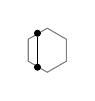
\begin{tikzpicture}[scale=1]
\node (h) [draw, color=gray, shape border rotate=30, minimum size=0.22in, regular polygon, regular polygon sides=6] at (0,0) {};
\node at (h.side 3) [draw,circle,fill,inner sep=0.75pt] (s1) {};
\node at (h.side 1) [draw,circle,fill,inner sep=0.75pt] (s2) {};
\draw (s1)--(s2);
\end{tikzpicture}
}

\newcommand{\transitiontwofive}{
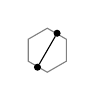
\begin{tikzpicture}[scale=1]
\node (h) [draw, color=gray, shape border rotate=30, minimum size=0.22in, regular polygon, regular polygon sides=6] at (0,0) {};
\node at (h.side 3) [draw,circle,fill,inner sep=0.75pt] (s1) {};
\node at (h.side 6) [draw,circle,fill,inner sep=0.75pt] (s2) {};
\draw (s1)--(s2);
\end{tikzpicture}
}

\newcommand{\transitiontwofour}{
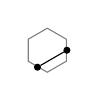
\begin{tikzpicture}[scale=1]
\node (h) [draw, color=gray, shape border rotate=30, minimum size=0.22in, regular polygon, regular polygon sides=6] at (0,0) {};
\node at (h.side 3) [draw,circle,fill,inner sep=0.75pt] (s1) {};
\node at (h.side 5) [draw,circle,fill,inner sep=0.75pt] (s2) {};
\draw (s1)--(s2);
\end{tikzpicture}
}

\newcommand{\transitionthreeone}{
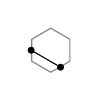
\begin{tikzpicture}[scale=1]
\node (h) [draw, color=gray, shape border rotate=30, minimum size=0.22in, regular polygon, regular polygon sides=6] at (0,0) {};
\node at (h.side 4) [draw,circle,fill,inner sep=0.75pt] (s1) {};
\node at (h.side 2) [draw,circle,fill,inner sep=0.75pt] (s2) {};
\draw (s1)--(s2);
\end{tikzpicture}
}

\newcommand{\transitionthreezero}{
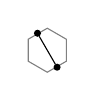
\begin{tikzpicture}[scale=1]
\node (h) [draw, color=gray, shape border rotate=30, minimum size=0.22in, regular polygon, regular polygon sides=6] at (0,0) {};
\node at (h.side 4) [draw,circle,fill,inner sep=0.75pt] (s1) {};
\node at (h.side 1) [draw,circle,fill,inner sep=0.75pt] (s2) {};
\draw (s1)--(s2);
\end{tikzpicture}
}

\newcommand{\transitionthreefive}{
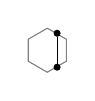
\begin{tikzpicture}[scale=1]
\node (h) [draw, color=gray, shape border rotate=30, minimum size=0.22in, regular polygon, regular polygon sides=6] at (0,0) {};
\node at (h.side 4) [draw,circle,fill,inner sep=0.75pt] (s1) {};
\node at (h.side 6) [draw,circle,fill,inner sep=0.75pt] (s2) {};
\draw (s1)--(s2);
\end{tikzpicture}
}

\newcommand{\transitionthreefour}{
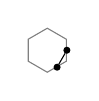
\begin{tikzpicture}[scale=1]
\node (h) [draw, color=gray, shape border rotate=30, minimum size=0.22in, regular polygon, regular polygon sides=6] at (0,0) {};
\node at (h.side 4) [draw,circle,fill,inner sep=0.75pt] (s1) {};
\node at (h.side 5) [draw,circle,fill,inner sep=0.75pt] (s2) {};
\draw (s1)--(s2);
\end{tikzpicture}
}

\newcommand{\transitionfourzero}{
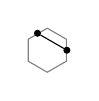
\begin{tikzpicture}[scale=1]
\node (h) [draw, color=gray, shape border rotate=30, minimum size=0.22in, regular polygon, regular polygon sides=6] at (0,0) {};
\node at (h.side 5) [draw,circle,fill,inner sep=0.75pt] (s1) {};
\node at (h.side 1) [draw,circle,fill,inner sep=0.75pt] (s2) {};
\draw (s1)--(s2);
\end{tikzpicture}
}

\newcommand{\transitionfourfive}{
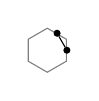
\begin{tikzpicture}[scale=1]
\node (h) [draw, color=gray, shape border rotate=30, minimum size=0.22in, regular polygon, regular polygon sides=6] at (0,0) {};
\node at (h.side 5) [draw,circle,fill,inner sep=0.75pt] (s1) {};
\node at (h.side 6) [draw,circle,fill,inner sep=0.75pt] (s2) {};
\draw (s1)--(s2);
\end{tikzpicture}
}


\newcommand{\growth}{
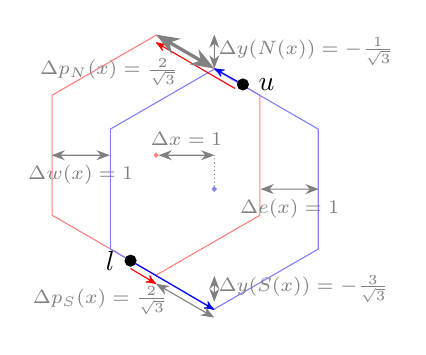
\begin{tikzpicture}[scale=1, transform shape]
\clip (1.3,-1) rectangle (6,2.8);

\node [draw, color=red!50, shape border rotate=30, minimum size=1.2in, regular polygon, regular polygon sides=6] at (2.93,1.18) (H1) {};

\node [draw,circle,fill,color=red!50,inner sep=0.5pt] at (2.93,1.18) (c1) {};

\node [draw, color=blue!50, shape border rotate=30, minimum size=1.2in, regular polygon, regular polygon sides=6] at (3.67,0.75) (H2) {};

\node [draw,circle,fill,color=blue!50,inner sep=0.5pt] at (3.67,0.75) (c2) {};


\node at (H2.side 6) [xshift=-0.3cm,yshift=0.18cm,draw,circle,fill,inner sep=1.4pt,label=0:{$u$}] (u) {};

\node at (H2.side 3) [xshift=-0.4cm,yshift=0.24cm,draw,circle,fill,inner sep=1.4pt,label=-180:{$l$}] (l) {};

\draw (u) -- (H2.corner 1) [->,>=stealth',blue];
\draw ($(u) + (-0.1cm,-0.052cm)$) -- ($(H1.corner 1) + (0,-0.1cm)$) [->,>=stealth',red];


\coordinate (c1r) at ($(c1)+(0:4)$);
\coordinate (c2u) at ($(c2)+(90:4)$);

\coordinate (z) at (intersection of c1--c1r and c2--c2u);

\draw [gray,<->,{Stealth-Stealth}] (c1) -- (z)  node [midway, above] {\scriptsize $\Delta x=1$};

\draw [densely dotted, gray] (c2) -- (z);

\coordinate (a) at (H1.corner 1);
\coordinate (b) at (H2.corner 1);

\draw [very thick,gray,<->,{Stealth-Stealth}] (a) -- (b)  node [midway, below left=-2pt] {\scriptsize $\Delta p_N(x)=\frac{2}{\sqrt{3}}$};

\coordinate (ar) at ($(a)+(0:4)$);
\coordinate (bu) at ($(b)+(90:4)$);

\coordinate (z) at (intersection of a--ar and b--bu);

\draw [gray,<->,{Stealth-Stealth}] (b) -- (z)  node [midway, right=-2pt] {\scriptsize $\Delta y(N(x)) = -\frac{1}{\sqrt{3}}$};


\coordinate (a) at (H1.side 2);
\coordinate (b) at (H2.side 2);

\coordinate (ar) at ($(a)+(0:4)$);
\coordinate (bu) at ($(b)+(90:4)$);

\coordinate (z) at (intersection of a--ar and b--bu);

\draw [gray,<->,{Stealth-Stealth}] (a) -- (z)  node [midway, below] {\scriptsize $\Delta w(x) = 1$};

\coordinate (a) at (H1.side 5);
\coordinate (b) at (H2.side 5);

\coordinate (ar) at ($(a)+(-90:4)$);
\coordinate (bu) at ($(b)+(180:4)$);

\coordinate (z) at (intersection of a--ar and b--bu);

\draw [gray,<->,{Stealth-Stealth}] (z) -- (b)  node [midway, below] {\scriptsize $\Delta e(x) = 1$};



\draw (l) -- (H2.corner 4) [->,>=stealth',blue];
\draw ($(l) + (0,-0.1cm)$) -- ($(H1.corner 4) + (0,-0.1cm)$) [->,>=stealth',red];

\coordinate (a) at (H1.corner 4);
\coordinate (b) at (H2.corner 4);

\draw [gray,<->,{Stealth-Stealth}] ($(H1.corner 4) + (0,-0.1cm)$) -- ($(H2.corner 4) + (0,-0.1cm)$)  node [midway, left=3pt] {\scriptsize $\Delta p_S(x)=\frac{2}{\sqrt{3}}$};

\coordinate (ar) at ($(a)+(0:4)$);
\coordinate (bu) at ($(b)+(90:4)$);

\coordinate (z) at (intersection of a--ar and b--bu);

\draw [gray,<->,{Stealth-Stealth}] ($(H2.corner 4) + (0,0.1cm)$) -- (z) node [midway, right=-2pt] {\scriptsize $\Delta y(S(x))=-\frac{3}{\sqrt{3}}$};
\end{tikzpicture}\hspace{-0.8cm}
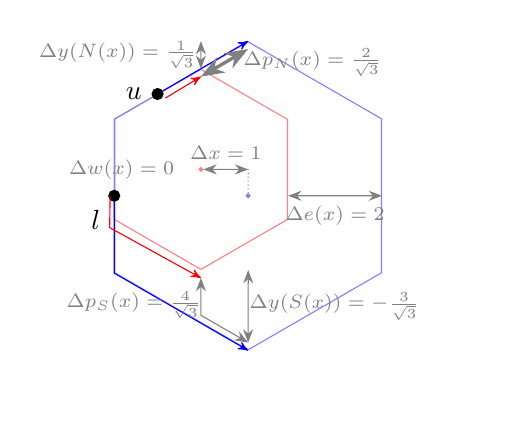
\begin{tikzpicture}[scale=1, transform shape]
\clip (0.5,-1.55) rectangle (6.5,3.1);

\node [draw, color=red!50, shape border rotate=30, minimum size=1in, regular polygon, regular polygon sides=6] at (2.7,1.3) (H1) {};

\node [draw,circle,fill,color=red!50,inner sep=0.5pt] at (2.7,1.3) (c1) {};

\node [draw, color=blue!50, shape border rotate=30, minimum size=1.54in, regular polygon, regular polygon sides=6] at (3.3,0.965) (H2) {};

\node [draw,circle,fill,color=blue!50,inner sep=0.5pt] at (3.3,0.965) (c2) {};


\node at (H2.side 1) [xshift=-0.3cm,yshift=-0.18cm,draw,circle,fill,inner sep=1.4pt,label=180:{$u$}] (u) {};

\node at (H2.side 2) [draw,circle,fill,inner sep=1.4pt,label=-135:{$l$}] (l) {};

\draw (u) -- (H2.corner 1) [->,>=stealth',blue];
\draw ($(u) + (0.1cm,-0.052cm)$) -- ($(H1.corner 1) + (0,-0.1cm)$) [->,>=stealth',red];


\coordinate (c1r) at ($(c1)+(0:4)$);
\coordinate (c2u) at ($(c2)+(90:4)$);

\coordinate (z) at (intersection of c1--c1r and c2--c2u);

\draw [gray,<->,{Stealth-Stealth}] (c1) -- (z)  node [midway, above] {\scriptsize $\Delta x=1$};

\draw [densely dotted, gray] (c2) -- (z);

\coordinate (a) at (H1.corner 1);
\coordinate (b) at (H2.corner 1);

\draw [very thick,gray,<->,{Stealth-Stealth}] ($(a) + (0,-0.1cm)$) -- ($(b) + (0,-0.1cm)$)  node [midway, right=3pt] {\scriptsize $\Delta p_N(x)=\frac{2}{\sqrt{3}}$};

\coordinate (ar) at ($(a)+(90:4)$);
\coordinate (bu) at ($(b)+(180:4)$);

\coordinate (z) at (intersection of a--ar and b--bu);

\draw [gray,<->,{Stealth-Stealth}] (a) -- (z)  node [midway, left=-2pt] {\scriptsize $\Delta y(N(x)) = \frac{1}{\sqrt{3}}$};


%\coordinate (a) at (H1.side 2);
%\coordinate (b) at (H2.side 2);

%\coordinate (ar) at ($(a)+(0:4)$);
%\coordinate (bu) at ($(b)+(90:4)$);

%\coordinate (z) at (intersection of a--ar and b--bu);

\node at ($(H1.side 2) + (0.1cm,0)$) [gray] {\scriptsize $\Delta w(x) = 0$};
%\draw [gray,<->,{Stealth-Stealth}] (a) -- (z)  node [midway, above] {\scriptsize $\Delta w(x) = 0$};

\coordinate (a) at (H1.side 5);
\coordinate (b) at (H2.side 5);

\coordinate (ar) at ($(a)+(-90:4)$);
\coordinate (bu) at ($(b)+(180:4)$);

\coordinate (z) at (intersection of a--ar and b--bu);

\draw [gray,<->,{Stealth-Stealth}] (z) -- (b)  node [midway, below] {\scriptsize $\Delta e(x) = 2$};

\draw (l) -- (H2.corner 3) -- (H2.corner 4) [->,>=stealth',blue];
\draw ($(l) + (-0.052cm,0)$) -- ($(H1.corner 3) + (-0.052cm,-0.1cm)$) -- ($(H1.corner 4) + (0,-0.1cm)$) [->,>=stealth',red];

\coordinate (a) at (H1.corner 4);
\coordinate (b) at (H2.corner 4);

\coordinate (ad) at ($(a)+(-90:4)$);
\coordinate (bl) at ($(b)+(150:4)$);

\coordinate (z) at (intersection of a--ad and b--bl);

\draw [gray,<->,{Stealth-Stealth}] ($(H1.corner 4) + (0,-0.1cm)$) -- ($(z) + (0,0.1cm)$) -- ($(H2.corner 4) + (0,0.1cm)$)  node [yshift=0.3cm, midway, left=5pt] {\scriptsize $\Delta p_S(x)=\frac{4}{\sqrt{3}}$};

\coordinate (ar) at ($(a)+(0:4)$);
\coordinate (bu) at ($(b)+(90:4)$);

\coordinate (z) at (intersection of a--ar and b--bu);

\draw [gray,<->,{Stealth-Stealth}] ($(H2.corner 4) + (0,0.1cm)$) -- (z) node [midway, right=-3pt] {\scriptsize $\Delta y(S(x))=-\frac{3}{\sqrt{3}}$};
\end{tikzpicture}\hspace{-1cm}
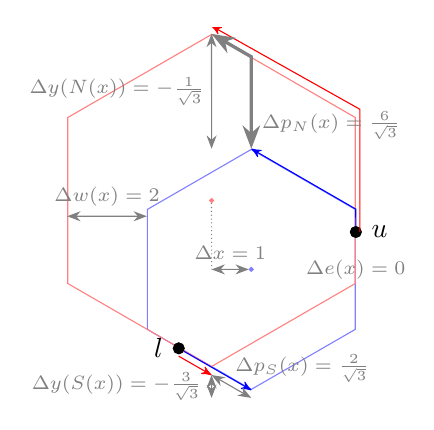
\begin{tikzpicture}[scale=1, transform shape]
\clip (1.1,-2.25) rectangle (5.9,2.5);

\node [draw, color=blue!50, shape border rotate=30, minimum size=1.2in, regular polygon, regular polygon sides=6] at (3.94,-0.57) (H2) {};

\node [draw,circle,fill,color=blue!50,inner sep=0.5pt] at (3.94,-0.57) (c1) {};

\node [draw, color=red!50, shape border rotate=30, minimum size=1.66in, regular polygon, regular polygon sides=6] at (3.435,0.305) (H1) {};

\node [draw,circle,fill,color=red!50,inner sep=0.5pt] at (3.435,0.305) (c2) {};


\node at (H1.side 5) [yshift=-0.4cm,draw,circle,fill,inner sep=1.4pt,label=0:{$u$}] (u) {};

\node at (H1.side 3) [xshift=0.5cm,yshift=-0.29cm,draw,circle,fill,inner sep=1.4pt,label=180:{$l$}] (l) {};

\draw ($(u) + (0.052cm,0cm)$) -- ($(H1.corner 6) + (0.052cm,0.1cm)$) -- ($(H1.corner 1) + (0,0.1cm)$) [->,>=stealth',red];
\draw (u) -- (H2.corner 6) -- (H2.corner 1) [->,>=stealth',blue];


\coordinate (c1r) at ($(c1)+(0:4)$);
\coordinate (c2u) at ($(c2)+(90:4)$);

\coordinate (z) at (intersection of c1--c1r and c2--c2u);

\draw [gray,<->,{Stealth-Stealth}] (c1) -- (z)  node [midway, above] {\scriptsize $\Delta x=1$};

\draw [densely dotted, gray] (c2) -- (z);

\coordinate (a) at (H1.corner 1);
\coordinate (b) at (H2.corner 1);


\coordinate (ar) at ($(a)+(-30:4)$);
\coordinate (bu) at ($(b)+(90:4)$);

\coordinate (z) at (intersection of a--ar and b--bu);

\draw [very thick,gray,<->,{Stealth-Stealth}] (a) -- (z) -- (b)  node [near end, right=0pt] {\scriptsize $\Delta p_N(x)=\frac{6}{\sqrt{3}}$};

\coordinate (ad) at ($(a)+(-90:4)$);
\coordinate (bl) at ($(b)+(180:4)$);

\coordinate (z) at (intersection of a--ad and b--bl);

\draw [gray,<->,{Stealth-Stealth}] (a) -- (z)  node [midway, left=-1pt] {\scriptsize $\Delta y(N(x)) = -\frac{1}{\sqrt{3}}$};


\node at (H2.side 5) [gray] {\scriptsize $\Delta e(x) = 0$};

\coordinate (a) at ($(H1.side 2) + (0,-0.2cm)$);
\coordinate (b) at (H2.side 2);

\coordinate (ar) at ($(a)+(0:4)$);
\coordinate (bu) at ($(b)+(90:4)$);

\coordinate (z) at (intersection of a--ar and b--bu);

\draw [gray,<->,{Stealth-Stealth}] (z) -- (a)  node [midway, above] {\scriptsize $\Delta w(x) = 2$};

\draw (l) -- (H2.corner 4) [->,>=stealth',blue];

\draw ($(l) + (0,-0.1cm)$) -- ($(H1.corner 4) + (0,-0.1cm)$) [->,>=stealth',red];

\coordinate (a) at (H1.corner 4);
\coordinate (b) at (H2.corner 4);

\draw [gray,<->,{Stealth-Stealth}] ($(H1.corner 4) + (0,-0.1cm)$) -- ($(H2.corner 4) + (0,-0.1cm)$)  node [midway, above right=-3pt] {\scriptsize $\Delta p_S(x)=\frac{2}{\sqrt{3}}$};

\coordinate (ad) at ($(a)+(-90:4)$);
\coordinate (bl) at ($(b)+(180:4)$);

\coordinate (z) at (intersection of a--ad and b--bl);

\draw [gray,<->,{Stealth-Stealth}] ($(H1.corner 4) + (0,-0.1cm)$) -- ($(z) + (0,-0.1cm)$) node [midway, left=0pt] {\scriptsize $\Delta y(S(x))=-\frac{3}{\sqrt{3}}$};


\end{tikzpicture}
%\begin{tikzpicture}[scale=1, transform shape]
%\clip (1,-2) rectangle (5.7,2.8);

%\node [draw, color=red!50, shape border rotate=30, minimum size=1.2in, regular polygon, regular polygon sides=6] at (2.93,1.18) (H1) {};

%\node [draw,circle,fill,color=red!50,inner sep=0.5pt] at (2.93,1.18) (c1) {};

%\node [draw, color=blue!50, shape border rotate=30, minimum size=1.66in, regular polygon, regular polygon sides=6] at (3.435,0.305) (H2) {};

%\node [draw,circle,fill,color=blue!50,inner sep=0.5pt] at (3.435,0.305) (c2) {};


%\node at (H2.side 6) [xshift=-0.5cm,yshift=0.29cm,draw,circle,fill,inner sep=1.4pt,label=0:{$u$}] (u) {};

%\node at (H2.side 2) [yshift=0.4cm,draw,circle,fill,inner sep=1.4pt,label=-135:{$l$}] (l) {};

%\draw (u) -- (H2.corner 1) [->,>=stealth',blue];
%\draw ($(u) + (-0.1cm,-0.052cm)$) -- ($(H1.corner 1) + (0,-0.1cm)$) [->,>=stealth',red];


%\coordinate (c1r) at ($(c1)+(0:4)$);
%\coordinate (c2u) at ($(c2)+(90:4)$);

%\coordinate (z) at (intersection of c1--c1r and c2--c2u);

%\draw [gray,<->,{Stealth-Stealth}] (c1) -- (z)  node [midway, above] {\scriptsize $\Delta(x)=1$};

%\draw [densely dotted, gray] (c2) -- (z);

%\coordinate (a) at (H1.corner 1);
%\coordinate (b) at (H2.corner 1);

%\draw [very thick,gray,<->,{Stealth-Stealth}] (a) -- (b)  node [midway, below left=-2pt] {\scriptsize $\Delta p_N(x)=\frac{2}{\sqrt{3}}$};

%\coordinate (ar) at ($(a)+(0:4)$);
%\coordinate (bu) at ($(b)+(90:4)$);

%\coordinate (z) at (intersection of a--ar and b--bu);

%\draw [gray,<->,{Stealth-Stealth}] (b) -- (z)  node [midway, right=-2pt] {\scriptsize $\Delta y(N(x)) = -\frac{1}{\sqrt{3}}$};


%\node at ($(H1.side 2) + (0.2cm,0)$) [gray] {\scriptsize $\Delta w(x) = 0$};

%\coordinate (a) at (H1.side 5);
%\coordinate (b) at (H2.side 5);

%\coordinate (ar) at ($(a)+(0:4)$);
%\coordinate (bu) at ($(b)+(90:4)$);

%\coordinate (z) at (intersection of a--ar and b--bu);

%\draw [gray,<->,{Stealth-Stealth}] (z) -- (a)  node [midway, below] {\scriptsize $\Delta e(x) = 2$};

%\draw (l) -- (H2.corner 3) -- (H2.corner 4) [->,>=stealth',blue];
%\draw ($(l) + (-0.052cm,0)$) -- ($(H1.corner 3) + (-0.052cm,-0.1cm)$) -- ($(H1.corner 4) + (0,-0.1cm)$) [->,>=stealth',red];

%\coordinate (a) at (H1.corner 4);
%\coordinate (b) at (H2.corner 4);

%\coordinate (ad) at ($(a)+(-90:4)$);
%\coordinate (bl) at ($(b)+(150:4)$);

%\coordinate (z) at (intersection of a--ad and b--bl);

%\draw [gray,<->,{Stealth-Stealth}] ($(H1.corner 4) + (0,-0.1cm)$) -- ($(z) + (0,0.1cm)$) -- ($(H2.corner 4) + (0,0.1cm)$)  node [midway, left=6pt] {\scriptsize $\Delta p_S(x)=\frac{6}{\sqrt{3}}$};

%\coordinate (ar) at ($(a)+(0:4)$);
%\coordinate (bu) at ($(b)+(90:4)$);

%\coordinate (z) at (intersection of a--ar and b--bu);

%\draw [gray,<->,{Stealth-Stealth}] ($(H2.corner 4) + (0,0.1cm)$) -- (z) node [midway, right=-2pt] {\scriptsize $\Delta y(S(x))=-\frac{5}{\sqrt{3}}$};
%\end{tikzpicture}
}





\newcommand{\badintervals}{
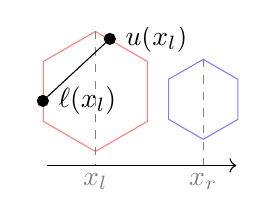
\begin{tikzpicture}[scale=1, transform shape]
\clip (.6,-.67) rectangle (3.3,1.4);

\node [draw, color=red!50, shape border rotate=30, minimum size=0.6in, regular polygon, regular polygon sides=6] at (1.46,0.59) (H1) {};

\coordinate (c1) at (1.46,0.59);

\node [draw, color=blue!50, shape border rotate=30, minimum size=0.4in, regular polygon, regular polygon sides=6] at (2.83,0.49) (H2) {};

\coordinate (c2) at (2.83,0.49);

\node at (H1.side 6) [xshift=-0.15cm,yshift=0.09cm,draw,circle,fill,inner sep=1.4pt,label=0:{$u(x_l)$}] (ul) {};

\node at (H1.side 2) [yshift=-0.12cm,draw,circle,fill,inner sep=1.4pt,label=0:{$\ell(x_l)$}] (l) {};

\draw [->] (0.85,-0.35) -- (3.25,-0.35);

\coordinate (N1) at (H1.corner 1);
\coordinate (N2) at (H2.corner 1);

\draw [gray, dashed] (N1) -- (1.46,-0.35);
\draw [gray, dashed] (N2) -- (2.83,-0.35);

\node at (1.46,-0.35) [label={[label distance=-0.15cm]-90:{\color{gray}{$x_l$}}}] {};
\node at (2.83,-0.35) [label={[label distance=-0.15cm]-90:{\color{gray}{$x_r$}}}] {};

\draw (ul) -- (l);

\end{tikzpicture}\hspace{0.75cm}
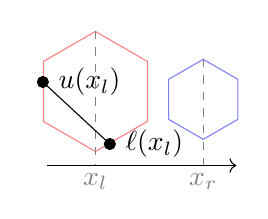
\begin{tikzpicture}[scale=1, transform shape]
\clip (.6,-.67) rectangle (3.3,1.4);

\node [draw, color=red!50, shape border rotate=30, minimum size=0.6in, regular polygon, regular polygon sides=6] at (1.46,0.59) (H1) {};

\coordinate (c1) at (1.46,0.59);

\node [draw, color=blue!50, shape border rotate=30, minimum size=0.4in, regular polygon, regular polygon sides=6] at (2.83,0.49) (H2) {};

\coordinate (c2) at (2.83,0.49);

\node at (H1.side 2) [yshift=0.12cm,draw,circle,fill,inner sep=1.4pt,label=0:{$u(x_l)$}] (ul) {};

\node at (H1.side 4) [xshift=-0.15cm,yshift=-0.09cm,draw,circle,fill,inner sep=1.4pt,label=0:{$\ell(x_l)$}] (l) {};

\draw [->] (0.85,-0.35) -- (3.25,-0.35);

\coordinate (N1) at (H1.corner 1);
\coordinate (N2) at (H2.corner 1);

\draw [gray, dashed] (N1) -- (1.46,-0.35);
\draw [gray, dashed] (N2) -- (2.83,-0.35);

\node at (1.46,-0.35) [label={[label distance=-0.15cm]-90:{\color{gray}{$x_l$}}}] {};
\node at (2.83,-0.35) [label={[label distance=-0.15cm]-90:{\color{gray}{$x_r$}}}] {};

\draw (ul) -- (l);

\end{tikzpicture}\hspace{0.75cm}
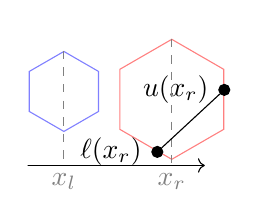
\begin{tikzpicture}[scale=1, transform shape]
\clip (1,-.67) rectangle (3.6,1.4);

\node [draw, color=red!50, shape border rotate=30, minimum size=0.6in, regular polygon, regular polygon sides=6] at (2.83,0.49) (H2) {};

\coordinate (c1) at (1.46,0.59);

\node [draw, color=blue!50, shape border rotate=30, minimum size=0.4in, regular polygon, regular polygon sides=6] at (1.46,0.59) (H1) {};

\coordinate (c2) at (2.83,0.49);

\node at (H2.side 5) [yshift=0.12cm,draw,circle,fill,inner sep=1.4pt,label=180:{$u(x_r)$}] (ul) {};

\node at (H2.side 3) [yshift=-0.09cm,xshift=0.15cm,draw,circle,fill,inner sep=1.4pt,label=180:{$\ell(x_r)$}] (l) {};

\draw [->] (0.85,-0.35) -- (3.25,-0.35);

\coordinate (N1) at (H1.corner 1);
\coordinate (N2) at (H2.corner 1);

\draw [gray, dashed] (N1) -- (1.46,-0.35);
\draw [gray, dashed] (N2) -- (2.83,-0.35);

\node at (1.46,-0.35) [label={[label distance=-0.15cm]-90:{\color{gray}{$x_l$}}}] {};
\node at (2.83,-0.35) [label={[label distance=-0.15cm]-90:{\color{gray}{$x_r$}}}] {};

\draw (ul) -- (l);

\end{tikzpicture}\hspace{0.75cm}
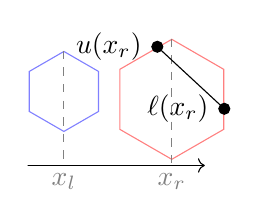
\begin{tikzpicture}[scale=1, transform shape]
\clip (1,-.67) rectangle (3.6,1.4);

\node [draw, color=red!50, shape border rotate=30, minimum size=0.6in, regular polygon, regular polygon sides=6] at (2.83,0.49) (H2) {};

\coordinate (c1) at (1.46,0.59);

\node [draw, color=blue!50, shape border rotate=30, minimum size=0.4in, regular polygon, regular polygon sides=6] at (1.46,0.59) (H1) {};

\coordinate (c2) at (2.83,0.49);

\node at (H2.side 1) [xshift=0.15cm,yshift=0.09cm,draw,circle,fill,inner sep=1.4pt,label=180:{$u(x_r)$}] (ul) {};

\node at (H2.side 5) [yshift=-0.12cm,draw,circle,fill,inner sep=1.4pt,label=180:{$\ell(x_r)$}] (l) {};

\draw [->] (0.85,-0.35) -- (3.25,-0.35);

\coordinate (N1) at (H1.corner 1);
\coordinate (N2) at (H2.corner 1);

\draw [gray, dashed] (N1) -- (1.46,-0.35);
\draw [gray, dashed] (N2) -- (2.83,-0.35);

\node at (1.46,-0.35) [label={[label distance=-0.15cm]-90:{\color{gray}{$x_l$}}}] {};
\node at (2.83,-0.35) [label={[label distance=-0.15cm]-90:{\color{gray}{$x_r$}}}] {};

\draw (ul) -- (l);

\end{tikzpicture}
}








\newcommand{\gentlepath}{
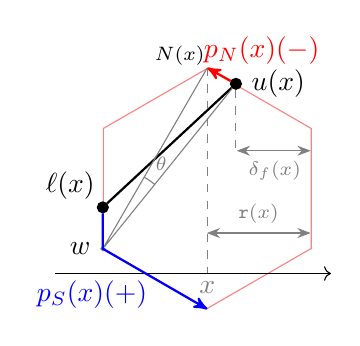
\begin{tikzpicture}[scale=1, transform shape]
%\clip (1.3,-1) rectangle (8,2.8);

\node [draw, color=red!50, shape border rotate=30, minimum size=1.2in, regular polygon, regular polygon sides=6] at (2.93,1.18) (H1) {};

\coordinate (c1) at (2.93,1.18);

\node at (H1.side 6) [xshift=-0.3cm,yshift=0.18cm,draw,circle,fill,inner sep=1.4pt,label={[label distance=0pt]0:$u(x)$}] (ul) {};

\node at ($(ul)+(0,-0.85)$) [inner sep=0pt,outer sep=-0.2pt] (x) {};
\draw [gray,<->,{Stealth-Stealth}] (x) -- ($(x)+(0.95,0)$) node [below left] {\scriptsize $\delta_f(x)$};

\draw [gray,dashed] (ul) -- (ul |- 1, 1.65);

\node at (H1.side 2) [yshift=-0.24cm,draw,circle,fill,inner sep=1.4pt,label={[label distance=-3pt]135:$\ell(x)$}] (l) {};

\draw [thick] (ul) -- (l);

\node at (H1.corner 3) [draw,gray,circle,fill,inner sep=0.5pt,label=-180:{$w$}] (w) {};

\draw [->] (1,0.1) -- (4.5,0.1);

\coordinate (N1) at (H1.corner 1);

\node at (N1) [label={[label distance=-0.3cm]135:{\scriptsize $N(x)$}}] {};

\draw [gray] (ul) -- (w) -- (N1);

\draw [gray, dashed] (N1) -- (2.93,0.1);

\draw pic [draw=gray, "\color{gray}{\scriptsize $\theta$}", angle eccentricity=1.25,angle radius=1.05cm] {angle = ul--w--N1};


\node at (2.93,0.1) [label={[label distance=-0.15cm]-90:{\color{gray}{$x$}}}] {};

\draw [gray,<->,{Stealth-Stealth},label=90:${\tt r}(x)$] ($(w)+(2.64,0.2)$$) -- ($(w)+(1.32,0.2)$) node [midway, above] {\scriptsize ${\tt r}(x)$};

\draw (l) -- (H1.corner 3) -- (H1.corner 4) [->,>=stealth',blue,thick];
\draw (ul) -- (H1.corner 1) [->,>=stealth',red,thick];
%\draw ($(l) + (-0.052cm,0)$) -- ($(H1.corner 3) + (-0.052cm,-0.1cm)$) -- ($(H1.corner 4) + (0,-0.1cm)$) [->,>=stealth',red];

\node at (H1.side 6) [red,xshift=0.75,yshift=0.6cm] {$p_N(x) (-)$};

\node at (H1.side 3) [blue,xshift=-0.8cm,yshift=-0.2cm] {$p_S(x) (+)$};


\end{tikzpicture}\hspace{1cm}
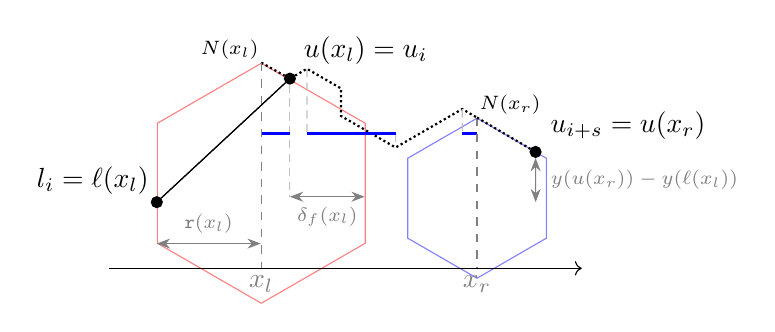
\begin{tikzpicture}[scale=1, transform shape]
%\clip (1.3,-1) rectangle (8,2.8);

\node [draw, color=red!50, shape border rotate=30, minimum size=1.2in, regular polygon, regular polygon sides=6] at (2.93,1.18) (H1) {};

\coordinate (c1) at (2.93,1.18);

\node [draw, color=blue!50, shape border rotate=30, minimum size=0.8in, regular polygon, regular polygon sides=6] at (5.67,0.99) (H2) {};

\coordinate (c2) at (5.67,0.99);

\node at (H1.side 6) [xshift=-0.3cm,yshift=0.18cm,draw,circle,fill,inner sep=1.4pt,label=45:{$u(x_l)=u_i$}] (ul) {};

\node at (H1.side 2) [yshift=-0.24cm,draw,circle,fill,inner sep=1.4pt,label={[label distance=-3pt]135:$l_i = \ell(x_l)$}] (l) {};



%\node at (H1.side 6) [xshift=-0.3cm,yshift=0.18cm,draw,circle,fill,inner sep=1.4pt,label=45:{$u(x_l)$}] (ul) {};

%\draw [gray,<->,{Stealth-Stealth},label=90:$\theta_f(x_l)$] ($(ul)+(0,-1.3)$) -- ($(ul)+(-0.36,-1.3)$) node [above right] {\scriptsize ${\tt r}(x_l)-\delta_f(x_l)$};

\draw [gray,<->,{Stealth-Stealth}] ($(ul)+(0,-1.5)$) -- ($(ul)+(0.95,-1.5)$) node [midway, below] {\scriptsize $\delta_f(x_l)$};

%\node at (H1.side 2) [yshift=-0.24cm,draw,circle,fill,inner sep=1.4pt,label=135:{$\ell(x_l)$}] (l) {};

%\node at (H2.side 6) [xshift=+0.3cm,yshift=-0.18cm,draw,circle,fill,inner sep=1.4pt,label=45:{$u_{i+s}=u(x_r)$}] (ur) {};

\node at (H1.corner 3) (w) {};

\draw [->] (1,0.1) -- (7,0.1);

\coordinate (N1) at (H1.corner 1);
\coordinate (N2) at (H2.corner 1);

%\draw (N1) -- ++(-30:0.65) -- ++(30:0.35) -- ++(-90:.25) -- ++ (-30:1.1) -- ++ (30:0.6);


\coordinate (N12) at ($(ul)+(30:0.25)$);
\coordinate (N13) at ($(N12)+(-30:0.5)$);
\coordinate (N14) at ($(N13)+(-90:.35)$);
\coordinate (N15) at ($(N14)+(-30:0.8)$);



%\draw [decorate,decoration={brace,amplitude=10pt},xshift=-4pt,yshift=0pt]
%(0.5,0.5) -- (0.5,5.0) node [black,midway,xshift=-0.6cm] 
%{\footnotesize $P_1$};

\coordinate (x) at ($(N15)+(30:.66)$);

\coordinate (xd) at ($(x)+(30:6)$);
\coordinate (N2d) at ($(N2)+(150:4)$);

\coordinate (z) at (intersection of N2--N2d and x--xd);

\draw [densely dotted,thick] (N1) -- (ul) -- (N12) -- (N13) -- (N14) -- (N15) -- (x) -- (z) -- (N2);



\coordinate (N1d) at ($(N1)+(-90:3)$);
\coordinate (ud) at ($(ul)+(-90:3)$);
\coordinate (N12d) at ($(N12)+(-90:3)$);
\coordinate (N15d) at ($(N15)+(-90:3)$);
\coordinate (zd) at ($(z)+(-90:3)$);
\coordinate (N2d) at ($(N2)+(-90:3)$);


\coordinate (N1b) at ($(N1)+(0,-0.9)$);
\coordinate (N1r) at ($(N1b)+(0:10)$);

\coordinate (z1) at (intersection of N1--N1d and N1b--N1r);
\coordinate (z2) at (intersection of ul--ud and N1b--N1r);
\coordinate (z3) at (intersection of N12--N12d and N1b--N1r);
\coordinate (z4) at (intersection of N15--N15d and N1b--N1r);
\coordinate (z5) at (intersection of z--zd and N1b--N1r);
\coordinate (z6) at (intersection of N2--N2d and N1b--N1r);

\draw [gray!50, densely dashed] (ul) -- ($(ul)+(0,-1.5)$);
\draw [gray!50, densely dashed] (N12) -- (z3);
\draw [gray!50, densely dashed] (z) -- (z5);
\draw [gray!50, densely dashed] (z4) -- (N15);


\draw [blue, very thick] (z1) -- (z2);
\draw [blue, very thick] (z3) -- (z4);
\draw [blue, very thick] (z5) -- (z6);





\node at (N1) [label={[label distance=-0.3cm]135:{\scriptsize $N(x_l)$}}] {};
\node at (N2) [label={[label distance=-0.3cm]45:{\scriptsize $N(x_r)$}}] {};

%\draw [gray] (ul) -- (w) -- (N1);

\draw [gray, dashed] (N1) -- (2.93,0.1);
\draw [gray, dashed] (N2) -- (5.67,0.1);

%\draw pic [draw=gray, "\color{gray}{\scriptsize $\Theta$}", angle eccentricity=1.25,angle radius=1.05cm] {angle = ul--w--N1};


\node at (2.93,0.1) [label={[label distance=-0.15cm]-90:{\color{gray}{$x_l$}}}] {};
\node at (5.67,0.1) [label={[label distance=-0.15cm]-90:{\color{gray}{$x_r$}}}] {};

\draw [gray,<->,{Stealth-Stealth},label=90:${\tt r}(x_l)$] ($(w)$) -- ($(w)+(1.32,0)$) node [midway, above] {\scriptsize ${\tt r}(x_l)$};


%\coordinate (lr) at ($(l)+(0:6)$);
%\coordinate (urd) at ($(ur)+(-90:4)$);

%\coordinate (z) at (intersection of l--lr and ur--urd);

%\draw [gray,<->,{Stealth-Stealth}] (ur) -- (z)  node [midway, right=2pt] {\scriptsize $y(u(x_r)) - y((x_l))$};

\draw (ul) -- (l);



\node at (H2.side 6) [xshift=+0.3cm,yshift=-0.18cm,draw,circle,fill,inner sep=1.4pt,label={[label distance=0pt]30:$u_{i+s} = u(x_r)$}] (ur) {};

\draw [densely dotted,thick] (N2) -- (ur);




\coordinate (lr) at ($(l)+(0:6)$);
\coordinate (urd) at ($(ur)+(-90:4)$);

\coordinate (z) at (intersection of l--lr and ur--urd);

\draw [gray,<->,{Stealth-Stealth}] (ur) -- (z)  node [midway, right=2pt] {\scriptsize $y(u(x_r)) - y(\ell(x_l))$};

\draw (ul) -- (l);

\end{tikzpicture}
}

\newcommand{\linearworstcase}{
\begin{tikzpicture}[scale=1, transform shape]
%\clip (1.3,-1) rectangle (8,2.8);

\node [draw, color=red!50, shape border rotate=30, minimum size=1.2in, regular polygon, regular polygon sides=6] at (2.93,1.18) (H1) {};

\coordinate (c1) at (2.93,1.18);

\node [draw, color=blue!50, shape border rotate=30, minimum size=0.8in, regular polygon, regular polygon sides=6] at (5.67,0.99) (H2) {};

\coordinate (c2) at (5.67,0.99);



\node at (H1.side 6) [xshift=-0.3cm,yshift=0.18cm,draw,circle,fill,inner sep=1.4pt,label=0:{$u(x_l)$}] (ul) {};

\draw [gray,<->,{Stealth-Stealth},label=90:$\theta_f(x_l)$] ($(ul)+(0,-1.1)$) -- ($(ul)+(0.96,-1.1)$) node [below left] {\scriptsize $\delta_f(x_l)$};

\draw [gray,<->,{Stealth-Stealth},label=90:$\theta_f(x_l)$] ($(ul)+(-0.96,-1.1)$) -- ($(ul)+(0,-1.1)$) node [below left] {\scriptsize $\delta_f(x_l)$};

\draw [gray, dashed] (ul) -- ($(ul)+(0,-1.1)$);


\node at (H1.side 2) [yshift=-0.24cm,draw,circle,fill,inner sep=1.4pt,label=180:{$\ell(x_l)$}] (l) {};

\draw [gray,<->,{Stealth-Stealth},label=90:$\theta_f(x_l)$] ($(l)+(0,-0.5)$) -- ($(l)+(0.36,-0.5)$) node [very near start, below] {\scriptsize ${\tt r}(x_l) - \delta_f(x_l)$};

% \draw [gray,<->,{Stealth-Stealth},label=90:$\theta_f(x_l)$] ($(l)+(0.36,-0.5)$) -- ($(l)+(0.72,-0.5)$) node [very near end, above] {\scriptsize $\theta_f(x)$};

%\draw [gray, dashed] ($(l)+(0.36,-0.1)$) -- ($(l)+(0.36,-0.5)$);

\node at (H2.side 5) [yshift=+0.18cm,draw,circle,fill,inner sep=1.4pt,label=45:{$u(x_r)$}] (ur) {};


%%%%%%%%%%%%%%%%%%%%%

\coordinate (N12) at ($(ul)+(30:0.25)$);

%\coordinate (N12d) at ($(N12)+(-90:3)$);
%\draw [gray, densely dashed] (N12) -- (N12d);

\coordinate (N13) at ($(N12)+(-30:0.35)$);
\coordinate (N14) at ($(N13)+(-90:.35)$);
\coordinate (N15) at ($(N14)+(-30:0.8)$);

%\coordinate (N15d) at ($(N15)+(-90:3)$);
%\draw [gray!50, densely dashed] (N15) -- (N15d);

\coordinate (x) at ($(N15)+(30:.66)$);

\coordinate (xd) at ($(x)+(30:6)$);
\coordinate (N2d) at ($(N2)+(150:4)$);

\coordinate (z) at (intersection of N2--N2d and x--xd);

\draw [densely dotted] (N1) -- (ul) -- (N12) -- (N13) -- (N14) -- (N15) -- (x) -- (z) -- (N2);





%\draw (ul) -- ++(-30:1) -- ++(30:0.5) -- ++(-30:.5) -- ++ (30:0.37) -- ++ (ur);

\draw [->] (1,0.1) -- (7,0.1);

\coordinate (N1) at (H1.corner 1);
\coordinate (N2) at (H2.corner 1);

%\node at (N1) [label={[label distance=-0.3cm]135:{\scriptsize $N(x_l)$}}] {};
%\node at (N2) [label={[label distance=-0.3cm]45:{\scriptsize $N(x_r)$}}] {};

%\draw [gray] (ul) -- (w) -- (N1);

\draw [gray, dashed] (N1) -- (2.93,0.1);
\draw [gray, dashed] (N2) -- (5.67,0.1);

%\draw pic [draw=gray, "\color{gray}{\scriptsize $\Theta$}", angle eccentricity=1.25,angle radius=1.05cm] {angle = ul--w--N1};


\node at (2.93,0.1) [label={[label distance=-0.15cm]-90:{\color{gray}{$x_l$}}}] {};
\node at (5.67,0.1) [label={[label distance=-0.15cm]-90:{\color{gray}{$x_r$}}}] {};

%\draw [blue,thick,<->,{Stealth-Stealth}] ($($(l)+(0.72,-0.1)$)$) -- ($($(l)+(2.36,0)$)+(2.59,-0.1)$) node [midway, above] {};

%\draw [red,thick,<->,{Stealth-Stealth},label=90:${\tt r}(x_l)$] ($($(l)+(0.36,-0.5)$)$) -- ($($(l)+(2.36,-0.5)$)+(1.7,0)$) node [midway, above] {};


\draw [blue,thick,<->,{Stealth-Stealth}] ($($(l)+(0.72,0)$)$) -- ($($(l)+(2.36,0.5)$)+(2.59,-0.5)$) node [midway, above] {};

\draw [red,thick,<->,{Stealth-Stealth},label=90:${\tt r}(x_l)$] ($($(l)+(0.36,-0.5)$)$) -- ($($(l)+(2.36,-0.5)$)+(1.7,0)$) node [midway, above] {};


%\coordinate (lr) at ($(l)+(0:6)$);
%\coordinate (urd) at ($(ur)+(-90:4)$);

%\coordinate (z) at (intersection of l--lr and ur--urd);

%\draw [gray,<->,{Stealth-Stealth}] (ur) -- (z)  node [midway, right=2pt] {\scriptsize $y(u(x_r)) - y((x_l))$};

\draw (ul) -- (l);
\end{tikzpicture}
\begin{tikzpicture}[scale=1, transform shape]
%\clip (1.3,-1) rectangle (8,2.8);

\node [draw, color=red!50, shape border rotate=30, minimum size=1.2in, regular polygon, regular polygon sides=6] at (2.93,1.18) (H1) {};

\coordinate (c1) at (2.93,1.18);

\node [draw, color=blue!50, shape border rotate=30, minimum size=0.8in, regular polygon, regular polygon sides=6] at (5.67,0.99) (H2) {};

\coordinate (c2) at (5.67,0.99);



\node at (H1.side 6) [xshift=-0.3cm,yshift=0.18cm,draw,circle,fill,inner sep=1.4pt,label=0:{$u(x_l)$}] (ul) {};

%\draw [gray,<->,{Stealth-Stealth},label=90:$\theta_f(x_l)$] ($(ul)+(0,-0.5)$) -- ($(ul)+(-0.36,-0.5)$) node [very near start, below] {\scriptsize $\theta_f(x_l)$};

\draw [gray,<->,{Stealth-Stealth},label=90:$\theta_f(x_l)$] ($(ul)+(0,-1.65)$) -- ($(ul)+(0.96,-1.65)$) node [below left] {\scriptsize $\delta_f(x_l)$};
\draw [gray,<->,{Stealth-Stealth},label=90:$\theta_f(x_l)$] ($(ul)+(-0.96,-1.65)$) -- ($(ul)+(0,-1.65)$) node [below left] {\scriptsize $\delta_f(x_l)$};


\draw [gray, dashed] (ul) -- ($(ul)+(0,-1.65)$);



\node at (H1.side 2) [yshift=-0.24cm,draw,circle,fill,inner sep=1.4pt,label=180:{$\ell(x_l)$}] (l) {};

%\draw [gray,<->,{Stealth-Stealth},label=90:$\theta_f(x_l)$] ($(l)+(0.36,-0.5)$) -- ($(l)+(0,-0.5)$) node [above right] {\scriptsize ${\tt r}(x_l) - \delta_f(x_l)$};

\node at (H2.corner 2) [draw,circle,fill,inner sep=1.4pt,label=0:{$u(x_r)$}] (ur) {};


%%%%%%%

\coordinate (N12) at ($(N1)+(-30:0.1)$);

%\coordinate (N12d) at ($(N12)+(-90:3)$);
%\draw [gray, densely dashed] (N12) -- (N12d);

\coordinate (N13) at ($(N12)+(-90:1)$);
%\coordinate (N14) at ($(N13)+(-30:1.85)$);
%\coordinate (N15) at ($(N14)+(-30:1.85)$);

%\coordinate (N15d) at ($(N15)+(-90:3)$);
%\draw [gray!50, densely dashed] (N15) -- (N15d);

%\coordinate (x) at ($(N13)+(-30:1.66)$);

\coordinate (xd) at ($(N13)+(-30:6)$);
\coordinate (N2d) at ($(N2)+(-150:4)$);

\coordinate (z) at (intersection of N2--N2d and N13--xd);

\draw [densely dotted] (N1) -- (N12) -- (N13) -- (z) -- (N2);

\coordinate (zd) at ($(z)+(0,-5)$);
\coordinate (N2d) at ($(N2)+(6,0)$);

\coordinate (zzz) at (intersection of zd--z and N2--N2d);

\draw [red,dashed,thick,<->,{Stealth-Stealth}] (N2) -- (zzz);

\draw [gray, dashed] (z) -- (zzz);





%\draw (ul) -- ++(-30:1) -- ++(30:0.5) -- ++(-30:.5) -- ++ (30:0.37) -- ++ (ur);

\draw [->] (1,0.1) -- (7,0.1);

\coordinate (N1) at (H1.corner 1);
\coordinate (N2) at (H2.corner 1);

%\node at (N1) [label={[label distance=-0.3cm]135:{\scriptsize $N(x_l)$}}] {};
%\node at (N2) [label={[label distance=-0.3cm]45:{\scriptsize $N(x_r)$}}] {};

%\draw [gray] (ul) -- (w) -- (N1);

\draw [gray, dashed] (N1) -- (2.93,0.1);

\draw [gray, dashed] (N2) -- (5.67,0.1);

%\draw pic [draw=gray, "\color{gray}{\scriptsize $\Theta$}", angle eccentricity=1.25,angle radius=1.05cm] {angle = ul--w--N1};


\node at (2.93,0.1) [label={[label distance=-0.15cm]-90:{\color{gray}{$x_l$}}}] {};
\node at (5.67,0.1) [label={[label distance=-0.15cm]-90:{\color{gray}{$x_r$}}}] {};

\draw [blue,thick,<->,{Stealth-Stealth}] ($($(l)+(0.72,-0.5)$)$) -- ($($(l)+(1.47,-0.5)$)+(1.7,0)$) node [midway, above] {};


%\coordinate (lr) at ($(l)+(0:6)$);
%\coordinate (urd) at ($(ur)+(-90:4)$);

%\coordinate (z) at (intersection of l--lr and ur--urd);

%\draw [gray,<->,{Stealth-Stealth}] (ur) -- (z)  node [midway, right=2pt] {\scriptsize $y(u(x_r)) - y((x_l))$};

\draw (ul) -- (l);
\end{tikzpicture} 
\vspace{-0.5cm}\center{(a) \hspace{2.6in} (b)}
}





\newcommand{\induction}{
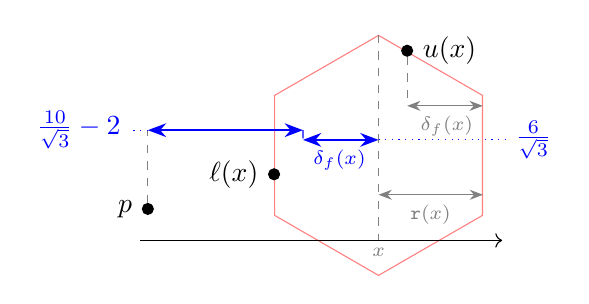
\begin{tikzpicture}[scale=1, transform shape]
%\clip (1.3,-1) rectangle (8,2.8);

\node at (0,0.5) [draw,circle,fill,inner sep=1.4pt,label=180:{$p$}] (p) {};
\coordinate (pu) at ($(p)+(0,1)$);

\draw [gray, dashed] (p) -- (pu);

\coordinate (c1) at (2.93,1.18);

\node [draw, color=red!50, shape border rotate=30, minimum size=1.2in, regular polygon, regular polygon sides=6] at (c1) (H1) {};

\node at (H1.side 6) [xshift=-0.3cm,yshift=0.18cm,draw,circle,fill,inner sep=1.4pt,label=0:{$u(x)$}] (ul) {};

\draw [gray,<->,{Stealth-Stealth}] ($(ul)+(0,-0.7)$) -- ($(ul)+(0.96,-0.7)$) node [below left] {\scriptsize $\delta_f(x)$};


\draw [gray, dashed] (ul) -- ($(ul)+(0,-0.7)$);


\node at (H1.side 2) [yshift=-0.24cm,draw,circle,fill,inner sep=1.4pt,label=180:{$\ell(x)$}] (l) {};

\coordinate (ld) at ($(l) + (0,-0.35)$);

%\draw [gray,<->,{Stealth-Stealth},label=90:$\theta_f(x)$] (ld) -- ($(ld)+(0.36,0)$) node [very near end, right] {\scriptsize $\theta_f(x)$};

%\coordinate (z) at ($(l)+(0.36,-0.35)$);
%\coordinate (z3) at ($(l)+(0.36,0.59)$);

%\draw [gray, dashed] (z2) -- (z);

\coordinate (z) at (1.97,1.5);
\coordinate (z2) at (2.93,1.377);

\draw [->] (-0.1,0.1) -- (4.5,0.1);

\coordinate (N1) at (H1.corner 1);

\draw [gray, dashed] (N1) -- (2.93,0.11);


\node at (2.93,0.1) [label={[label distance=-0.15cm]-90:{\color{gray}{{\scriptsize $x$}}}}] {};

\draw [blue,thick,<->,{Stealth-Stealth}] (pu) -- (z) node [midway, above] {};
\draw [blue,dotted](pu) -- ($(pu)+(-0.25,0)$) node [label={[label distance=-0.15cm]180:$\frac{10}{\sqrt{3}} - 2$}]{};

\draw [blue,thick,<->,{Stealth-Stealth}] (z2) -- ($(z2)+(-0.96,0)$) node [below right] {\scriptsize $\delta_f(x)$};
\draw [blue,dotted](z2) -- ($(z2)+(1.64,0)$) node [label={[label distance=-0.15cm]0:$\frac{6}{\sqrt{3}}$}]{};

\draw [blue, dashed] (z) -- ($(z2) + (-0.96,0)$);

%\coordinate (wx) at ($(H1.corner 3) + (0,-0.305)$);
%\draw [dashed,gray] (H1.corner 3) -- (wx); 
%\node at (wx) [label={[label distance=-0.125cm,gray]-90:{{\scriptsize $w(x)$}}}] {};

%\coordinate (ex) at ($(H1.corner 5) + (0,-0.305)$);
%\draw [dashed,gray] (H1.corner 5) -- (ex); 
%\node at (ex) [label={[label distance=-0.125cm,gray]-90:{{\scriptsize $e(x)$}}}] {};

%\draw [gray,<->,{Stealth-Stealth}] ($(ul)+(0,-1.5)$) -- ($(ul)+(0.95,-1.5)$) node [midway, below] {\scriptsize ${\tt r}(x_l)-\theta_f(x_l)$};
\draw [gray,<->,{Stealth-Stealth}] ($(H1.side 5)+(0,-.5)$) -- ($(c1)+(0,-.5)$) node [midway, below] {\scriptsize ${\tt r}(x)$};

\end{tikzpicture}\hspace{0.65cm}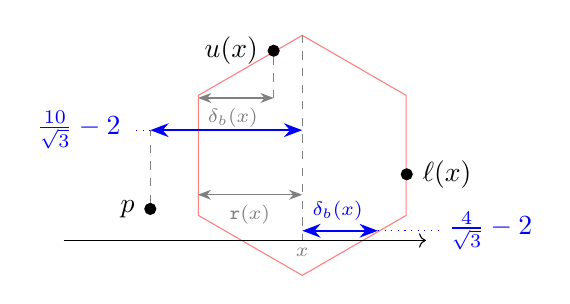
\begin{tikzpicture}[scale=1, transform shape]
%\clip (1.3,-1) rectangle (8,2.8);

\node at (1,0.5) [draw,circle,fill,inner sep=1.4pt,label=180:{$p$}] (p) {};
\coordinate (pu) at ($(p)+(0,1)$);

\draw [gray, dashed] (p) -- (pu);

\coordinate (c1) at (2.93,1.18);

\coordinate (z) at (2.93, 1.5);
\coordinate (z3) at (3.89, .223);

\node [draw, color=red!50, shape border rotate=30, minimum size=1.2in, regular polygon, regular polygon sides=6] at (c1) (H1) {};

\node at (H1.side 1) [xshift=0.3cm,yshift=0.18cm,draw,circle,fill,inner sep=1.4pt,label=180:{$u(x)$}] (ul) {};

\draw [gray,<->,{Stealth-Stealth}] ($(ul)+(0,-0.6)$) -- ($(ul)+(-0.96,-0.6)$) node [below right] {\scriptsize $\delta_b(x)$};


\draw [gray, dashed] (ul) -- ($(ul)+(0,-0.6)$);


\node at (H1.side 5) [yshift=-0.24cm,draw,circle,fill,inner sep=1.4pt,label=0:{$\ell(x)$}] (l) {};

\coordinate (ld) at ($(l) + (0,+0.35)$);

%\draw [gray,<->,{Stealth-Stealth},label=0:$\theta_b(x)$] (ld) -- ($(l)+(-0.36,0.35)$) node [very near start, above right] {\scriptsize $\theta_b(x)$};

%\coordinate (z) at ($(l)+(-0.36,+0.35)$);
%\coordinate (z2) at ($(l)+(-0.36,0.35)$);

%\draw [gray, dashed] (z2) -- (z3);


\draw [->] (-0.1,0.1) -- (4.5,0.1);

\coordinate (N1) at (H1.corner 1);

\draw [gray, dashed] (N1) -- (2.93,0.11);


\node at (2.93,0.1) [label={[label distance=-0.15cm]-90:{\color{gray}{{\scriptsize $x$}}}}] {};

\draw [blue,thick,<->,{Stealth-Stealth}] (pu) -- (z) node [midway, above] {};
\draw [blue,dotted](pu) -- ($(pu)+(-0.25,0)$) node [very near start, label={[label distance=0.1cm]180:$\frac{10}{\sqrt{3}} - 2$}]{};

\draw [blue,thick,<->,{Stealth-Stealth}] (z3) -- ($(z3)+(-0.96,0)$)  node [above right] {\scriptsize $\delta_b(x)$};
\draw [blue,dotted](z3) -- ($(z3)+(.8,0)$) node [label={[label distance=-0.15cm]0:$\frac{4}{\sqrt{3}}-2$}]{};

%\coordinate (wx) at ($(H1.corner 3) + (0,-0.305)$);
%\draw [dashed,gray] (H1.corner 3) -- (wx); 
%\node at (wx) [label={[label distance=-0.125cm,gray]-90:{{\scriptsize $w(x)$}}}] {};

% \coordinate (ex) at ($(H1.corner 5) + (0,-0.305)$);
% \draw [dashed,gray] (H1.corner 5) -- (ex); 
% \node at (ex) [label={[label distance=-0.125cm,gray]-90:{{\scriptsize $e(x)$}}}] {};

%\draw [gray,<->,{Stealth-Stealth}] ($(ul)+(0,-1.5)$) -- ($(ul)+(0.95,-1.5)$) node [midway, below] {\scriptsize ${\tt r}(x_l)-\theta_f(x_l)$};
\draw [gray,<->,{Stealth-Stealth}] ($(H1.side 2)+(0,-.5)$) -- ($(c1)+(0,-.5)$) node [midway, below] {\scriptsize ${\tt r}(x)$};

\end{tikzpicture}
\center{(a) \hspace{2.6in} (b)}

}



\newcommand{\proofA}{
\center\begin{tikzpicture}[scale=1, transform shape]
%\clip (1.3,-1) rectangle (8,2.8);


\draw [->] (1,0.1) -- (6.4,0.1);

\node at (0,0.5) [draw,circle,fill,inner sep=1.4pt,label=180:{$p$}] (p) {};
\coordinate (pu) at ($(p)+(0,1)$);

\draw [gray, dashed] (p) -- (pu);

\coordinate (c1) at (2.93,1.18);

\node [draw, color=red!50, shape border rotate=30, minimum size=1.2in, regular polygon, regular polygon sides=6] at (c1) (H1) {};

\node at (H1.side 6) [xshift=-0.3cm,yshift=0.18cm,draw,circle,fill,inner sep=1.4pt,label=45:{$u(x_l)$}] (ul) {};

\draw [gray,<->,{Stealth-Stealth}] ($(ul)+(0,-0.8)$) -- ($(ul)+(0.96,-0.8)$) node [above left] {\scriptsize $\delta_f(x_l)$};


\draw [gray, dashed] (ul) -- ($(ul)+(0,-0.6)$);


\node at (H1.side 2) [yshift=-0.24cm,draw,circle,fill,inner sep=1.4pt,label=180:{$\ell(x_l)$}] (l) {};

%\coordinate (ld) at ($(l) + (0,-0.35)$);

%\draw [gray,<->,{Stealth-Stealth},label=90:$\theta_f(x_l)$] (ld) -- ($(ld)+(0.36,0)$) node [very near end, right] {\scriptsize $\theta_f(x_l)$};

%\coordinate (z) at ($(l)+(0.36,-0.35)$);
\coordinate (z) at (1.97, 1.5);
\coordinate (z2) at (1.97, 1.38);
\coordinate (z3) at (2.93, 1.38);
\coordinate (z4) at (2.93, 1.5);
%\coordinate (z3) at ($(l)+(0.36,0.44)$);
%\coordinate (z4) at ($(l)+(0.36,-.7)$);

\draw [gray, dashed] (z) -- (z2);


%\draw [->] (-0.1,0.1) -- (4.5,0.1);

\coordinate (N1) at (H1.corner 1);

\draw [gray, dashed] (N1) -- (2.93,0.11);


\node at (2.93,0.1) [label={[label distance=-0.15cm]-90:{\color{gray}{{\scriptsize $x_l$}}}}] {};

\draw [blue,thick,<->,{Stealth-Stealth}] ($(z)+(-1.96,0)$) -- (z) node [midway, above] {};
\draw [blue,dotted]($(z)+(-2.1,0)$) -- ($(z)+(-2,0)$) node [label={[label distance=-0.1cm]180:$\frac{10}{\sqrt{3}} - 2$}]{};

\draw [blue,thick,<->,{Stealth-Stealth}] (z2) -- (z3) node [below left] {\scriptsize $\delta_f(x_l)$};

%\coordinate (wx) at ($(H1.corner 3) + (0,-0.305)$);
%\draw [dashed,gray] (H1.corner 3) -- (wx); 
%\node at (wx) [label={[label distance=-0.125cm,gray]-90:{{\scriptsize $w(x_l)$}}}] {};

%\coordinate (ex) at ($(H1.corner 5) + (0,-0.305)$);
%\draw [dashed,gray] (H1.corner 5) -- (ex); 
%\node at (ex) [label={[label distance=-0.125cm,gray]-90:{{\scriptsize $e(x)$}}}] {};

%\draw [gray,<->,{Stealth-Stealth}] ($(ul)+(0,-1.5)$) -- ($(ul)+(0.95,-1.5)$) node [midway, below] {\scriptsize ${\tt r}(x_l)-\theta_f(x_l)$};
\draw [gray,<->,{Stealth-Stealth}] ($(H1.side 5)+(0,-.5)$) -- ($(c1)+(0,-.5)$) node [midway, above] {\scriptsize ${\tt r}(x_l)$};

\node [draw, color=blue!50, shape border rotate=30, minimum size=0.8in, regular polygon, regular polygon sides=6] at (5.67,0.99) (H2) {};

\coordinate (c2) at (5.67,0.99);


\coordinate (z5) at (4.78, 1.5);
\coordinate (z6) at (4.78, 1.38);
\coordinate (z7) at (5.67, 1.38);

\draw [red,thick,<->,{Stealth-Stealth}] (z4) -- (z5);

\draw [blue,dotted](z) -- (z4) node {};


\draw [red,dotted](z7) -- (z3) node {};
\draw [red,dotted](z7) -- ($(z7)+(1,0)$) node [label={[label distance=-0.15cm]0:$\frac{6}{\sqrt{3}}$}]{};


%\node at (H2.corner 2) [draw,circle,fill,inner sep=1.4pt,label=90:{$u(x_r)$}] (ur) {};

\node at (5.67,0.1) [label={[label distance=-0.2cm]-45:{\color{gray}{{\scriptsize $x_r$}}}}] {};
\draw [gray, dashed] (N2) -- (5.67,0.1);

\draw [red,thick,<->,{Stealth-Stealth}] (z6) -- (z7) node [below left] {\scriptsize ${\tt r}(x_r)$};

%\draw [red,dotted] ($(l)+(0.36,-0.7)+(1.7,0)$$) -- ($(l)+(1.47,-0.7)+(1.7,0)+(1.6,0)$) node [label={[label distance=-0.2cm]0:$\frac{4}{\sqrt{3}}-2$}]{};

\coordinate (rwx) at ($(H2.corner 3) + (0,-0.37)$);
\draw [dashed,gray] (H2.corner 3) -- (rwx); 
\node at (rwx) [label={[label distance=-0.125cm,gray]-90:{{\scriptsize $w(x_r)$}}}] {};

\end{tikzpicture}
}



\newcommand{\proofB}{
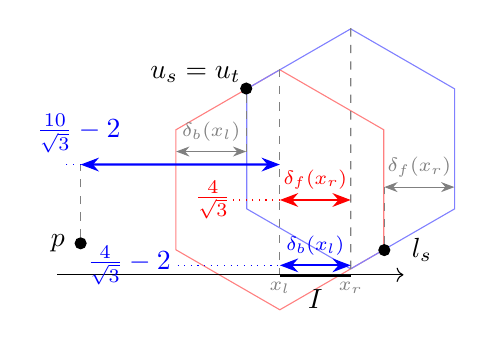
\begin{tikzpicture}[scale=1, transform shape]
%\clip (1.3,-1) rectangle (8,2.8);

\node at (0.4,0.5) [draw,circle,fill,inner sep=1.4pt,label=180:{$p$}] (p) {};
\coordinate (pu) at ($(p)+(0,1)$);

\draw [gray, dashed] (p) -- (pu);

\coordinate (c1) at (2.93,1.18);
\coordinate (c2) at ($(c1)+(.9,.5196)$);

%\coordinate (z1) at (1.93, 1.5);

\node [draw, color=red!50, shape border rotate=30, minimum size=1.2in, regular polygon, regular polygon sides=6] at (c1) (H1) {};

\node [draw, color=blue!50, shape border rotate=30, minimum size=1.2in, regular polygon, regular polygon sides=6] at (c2) (H2) {};

 \node at (H2.corner 2) [draw,circle,fill,inner sep=1.4pt,label={[label distance=-0.15cm]135:{$u_s=u_t$}}] (u) {};

 \node at (H1.corner 5) [draw,circle,fill,inner sep=1.4pt,label={[label distance=0.15cm]0:$l_s$}] (l) {};


\coordinate (N1) at (H1.corner 1);
\coordinate (N1x) at (2.93,0.1);

\draw [gray, dashed] (N1) -- (N1x);


\node at (N1x) [label={[label distance=-0.15cm]-90:{\color{gray}{{\scriptsize $x_l$}}}}] {};

\coordinate (N2) at (H2.corner 1);
\coordinate (N2x) at (3.83,0.1);

\draw [gray, dashed] (N2) -- (N2x);

\node at (N2x) [label={[label distance=-0.15cm]-90:{\color{gray}{{\scriptsize $x_r$}}}}] {};

\draw [gray,<->,{Stealth-Stealth}] ($(u)+(0,-0.8)$) -- ($(u)+(-0.89,-0.8)$) node [midway,above] {\scriptsize $\delta_b(x_l)$};
\draw [gray, dashed] (u) -- ($(u)+(0,-0.8)$);

\draw [gray,<->,{Stealth-Stealth}] ($(l)+(0,0.8)$) -- ($(l)+(0.89,+0.8)$) node [midway,above] {\scriptsize $\delta_f(x_r)$};
\draw [gray, dashed] (l) -- ($(l)+(0,0.8)$);




\coordinate (pr) at ($(pu)+(0:6)$);
\coordinate (w1) at (H1.side 2);
\coordinate (w1u) at ($(w1)+(90:6)$);
\coordinate (ud) at ($(u)+(-90:6)$);
\coordinate (lu) at ($(l)+(90:6)$);

\coordinate (z1) at (intersection of w1--w1u and pu--pr);
\coordinate (z3) at (intersection of u--ud and pu--pr);
\coordinate (z4) at (intersection of N1--N1x and pu--pr);
\coordinate (z2) at ($(z1)+(z4)-(z3)$);
\coordinate (z5) at (intersection of N2--N2x and pu--pr);
\coordinate (z6) at (intersection of l--lu and pu--pr);

%\draw [gray,<->,{Stealth-Stealth}] ($(z1)+(0,-0.4)$) -- ($(z2)+(0,-0.4)$) node [near start, below] {\scriptsize $\theta_b(x_l)$};

%\draw [gray,<->,{Stealth-Stealth}] ($(z3)+(0,.4)$) -- ($(z4)+(0,.4)$) node [midway,label={[label distance=-.17cm]10:{\color{gray}{{\scriptsize $\theta_b(x_l)$}}}}] {};

%\draw [gray,<->,{Stealth-Stealth}] ($(z5)+(0,.4)$) -- ($(z6)+(0,.4)$) node [midway,label={[label distance=-0.25cm]45:{\color{gray}{{\scriptsize $\theta_f(x_r)$}}}}] {};

%\coordinate (z) at ($(n1)!.5!(n2) + (0.6,0.4)$);
%\node at (z) [label={[label distance=-0.15cm]90:{\color{gray}{{\scriptsize $\theta_b(x_l)=\theta_f(x_r)$}}}}] {};

%\draw [gray,dotted,->,>=Stealth] (n1) -- (z);


%\draw [gray, dashed] (z2) -- ($(z2)+(0,-0.4)$);

\coordinate (o) at (0.1,0.1);
\coordinate (x) at (4.5,0.1);
\draw [->] (o) -- (x);

\draw [very thick] ($(z4)+(0,-1.41)$) -- ($(z5)+(0,-1.41)$) node [midway, label={[label distance=-0.1cm]-90:$I$}]{};

\draw [blue,thick,<->,{Stealth-Stealth}] (pu) -- (z4) node [midway, above] {};
\draw [blue,dotted](pu) -- ($(pu)+(-0.2,0)$) node [very near start, label={[label distance=-0.1cm]90:$\frac{10}{\sqrt{3}} - 2$}]{};

\draw [blue,thick,<->,{Stealth-Stealth}] ($(z4)+(0,-1.28)$) -- ($(z5)+(0,-1.28)$) node [midway,above] {\scriptsize $\delta_b(x_l)$};
\draw [blue,dotted]($(z4)+(-1.3,-1.28)$) -- ($(z4)+(0,-1.28)$) node [very near start,label={[label distance=0cm]180:$\frac{4}{\sqrt{3}}-2$}]{};

\draw [red,thick,<->,{Stealth-Stealth}] ($(z4)+(0,-.45)$) -- ($(z5)+(0,-.45)$) node [midway,above] {\scriptsize $\delta_f(x_r)$};
\draw [red,dotted]($(z4)+(0,-.45)$) -- ($(z4)+(-.6,-.45)$) node [very near end, label={[label distance=-0.15cm]180:$\frac{4}{\sqrt{3}}$}]{};

\coordinate (e) at (H1.corner 5);
\coordinate (ed) at ($(e) + (0,-1)$);
\coordinate (ex) at (intersection of o--x and e--ed);

\coordinate (w) at (H2.corner 3);
\coordinate (wd) at ($(w) + (0,-1)$);
\coordinate (wx) at (intersection of o--x and w--wd);


% \draw [dashed,gray] (e) -- (ex); 
% \node at (ex) [label={[label distance=-0.35cm,gray]-40:{{\scriptsize $e(x_l)$}}}] {};
% 
% \draw [dashed,gray] (w) -- (wx); 
% \node at (wx) [label={[label distance=-0.35cm,gray]-135:{{\scriptsize $w(x_r)$}}}] {};

%\draw [gray,<->,{Stealth-Stealth}] ($(ul)+(0,-1.5)$) -- ($(ul)+(0.95,-1.5)$) node [midway, below] {\scriptsize ${\tt r}(x_l)-\theta_f(x_l)$};
%\draw [gray,<->,{Stealth-Stealth}] ($(H1.side 2)+(0,-.5)$) -- ($(c1)+(0,-.5)$) node [midway, below] {\scriptsize ${\tt r}(x)$};

\end{tikzpicture}\hspace{0.6cm}
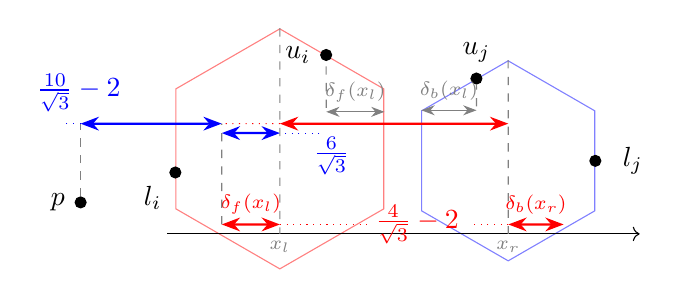
\begin{tikzpicture}
\coordinate (c1) at (2.93,1.18);
\coordinate (c2) at ($(c1)+(2.9,-.15196)$);

\node [draw, color=red!50, shape border rotate=30, minimum size=1.2in, regular polygon, regular polygon sides=6] at (c1) (H1) {};

\node [draw, color=blue!50, shape border rotate=30, minimum size=1in, regular polygon, regular polygon sides=6] at (c2) (H2) {};

 \node at (H1.side 6) [draw,shift={+(-0.075,0.0433cm)},circle,fill,inner sep=1.4pt,label={[label distance=0]180:{$u_i$}}] (ui) {};

 \node at (H1.side 2) [draw,yshift=-0.3cm,circle,fill,inner sep=1.4pt,label={[label distance=0cm]-135:$l_i$}] (li) {};

 \node at (H2.side 1) [draw,shift={+(0.15,0.0866cm)},circle,fill,inner sep=1.4pt,label={[label distance=0]90:{$u_j$}}] (uj) {};

 \node at (H2.side 5) [draw,circle,fill,inner sep=1.4pt,label={[label distance=0.15cm]0:$l_j$}] (lj) {};

\coordinate (o) at (1.5,0.1);
\coordinate (x) at (7.5,0.1);
\draw [->] (o) -- (x);

\coordinate (N1) at (H1.corner 1);
\coordinate (N1d) at ($(N1)+(-90:4)$);
\coordinate (N1x) at (intersection of o--x and N1--N1d);

\draw [gray, dashed] (N1) -- (N1x);

\node at (N1x) [label={[label distance=-0.15cm]-90:{\color{gray}{{\scriptsize $x_l$}}}}] {};

\coordinate (N2) at (H2.corner 1);
\coordinate (N2d) at ($(N2)+(-90:4)$);
\coordinate (N2x) at (intersection of o--x and N2--N2d);


\draw [gray, dashed] (N2) -- (N2x);

\node at (N2x) [label={[label distance=-0.15cm]-90:{\color{gray}{{\scriptsize $x_r$}}}}] {};

\node at (0.4,0.5) [draw,circle,fill,inner sep=1.4pt,label=180:{$p$}] (p) {};
\coordinate (pu) at ($(p)+(0,1)$);
\coordinate (pu2) at ($(p)+(0,0.88)$);
\coordinate (pu3) at ($(p)+(0,-0.28)$);
\draw [gray, dashed] (p) -- (pu);

\coordinate (pr) at ($(pu)+(0:6)$);
\coordinate (p2r) at ($(pu2)+(0:6)$);
\coordinate (p3r) at ($(pu3)+(0:6)$);

\coordinate (liu) at ($(li)+(90:6)$);
\coordinate (lid) at ($(li)+(-90:6)$);
\coordinate (uid) at ($(ui)+(-90:6)$);
\coordinate (ujd) at ($(uj)+(-90:6)$);
\coordinate (lju) at ($(lj)+(90:6)$);
\coordinate (ljd) at ($(lj)+(-90:6)$);

\coordinate (z1) at (intersection of li--liu and pu--pr);
\coordinate (z3) at (intersection of N1--N1x and pu--pr);
\coordinate (z4) at (intersection of ui--uid and pu--pr);
\coordinate (z2) at ($(z1)+(z4)-(z3)$);

\draw [blue,thick,<->,{Stealth-Stealth}] (pu) -- (z2) node [midway, above] {};
\draw [blue,dotted](pu) -- ($(pu)+(-0.2,0)$) node [very near start, label={[label distance=-0.1cm]90:$\frac{10}{\sqrt{3}} - 2$}]{};


\coordinate (z2d) at ($(z2)+(-90:6)$);
\coordinate (z5) at (intersection of z2--z2d and pu2--p2r);
\coordinate (z6) at (intersection of N1--N1x and pu2--p2r);

\draw [blue,thick,<->,{Stealth-Stealth}] (z5) -- (z6);
\draw [blue,dotted]($(z6)+(0.5,0)$) -- ($(z6)+(0,0)$) node [very near start,label={[label distance=-0.30cm]-30:$\frac{6}{\sqrt{3}}$}]{};

\coordinate (z7) at (intersection of N2--N2x and pu--pr);

\draw [red,thick,<->,{Stealth-Stealth}] (z3) -- (z7) node {};
\draw [red,dotted](z3) -- (z2) node {};

\coordinate (z8) at (intersection of z2--z2d and pu3--p3r);
\coordinate (z9) at (intersection of N1--N1x and pu3--p3r);

\draw [red,thick,<->,{Stealth-Stealth}] (z8) -- (z9) node [midway,above] {\scriptsize $\delta_f(x_l)$};
\draw [red,dotted]($(z9)+(0,0)$) -- ($(z9)+(1.1,0)$) node [very near end, label={[label distance=0.]0:$\frac{4}{\sqrt{3}}-2$}]{};
 


\coordinate (z10) at (intersection of uj--ujd and pu3--p3r);
\coordinate (z11) at (intersection of N2--N2x and pu3--p3r);
\coordinate (z12) at (intersection of lj--ljd and pu3--p3r);
\coordinate (z13) at ($(z12)-(z11)+(z10)$);

\draw [red,thick,<->,{Stealth-Stealth}] (z11) -- (z13) node [midway,above] {\scriptsize $\delta_b(x_r)$};
\draw [red,dotted]($(z11)+(0,0)$) -- ($(z11)+(-.5,0)$);

\coordinate (z13u) at ($(z13)+(90:6)$);

%\draw [red,dotted]($(z13)+(0,-.45)$) -- ($(z13)+(-.6,-.45)$) node [very near end, label={[label distance=-0.15cm]180:$\frac{4}{\sqrt{3}}-2$}]{};


\draw [gray,<->,{Stealth-Stealth}] ($(z4)+(0.74,0.15)$) -- ($(z4)+(0,0.15)$) node [midway,above] {\scriptsize $\delta_f(x_l)$};
%\draw [gray,<->,{Stealth-Stealth}] ($(z1)+(0,-0.25)$) -- ($(z2)+(0,-0.25)$) node [very near end,label={[label distance=-.1cm]-90:{\color{gray}{{\scriptsize $\theta_f(x_l)$}}}}] {};
%\draw [gray,<->,{Stealth-Stealth}] ($(z12)+(0,0.25)$) -- ($(z13)+(0,0.25)$) node [very near end,label={[label distance=-.1cm]92:{\color{gray}{{\scriptsize $\theta_b(x_l)$}}}}] {};
\draw [gray,<->,{Stealth-Stealth}] ($(z10)+(0,1.45)$) -- ($(z10)+(-0.7,1.45)$) node [midway, above]{\scriptsize $\delta_b(x_l)$};


\draw [gray, dashed] (z8) -- (z2);
\draw [gray, dashed] ($(z4)+(0,0.2)$) -- (ui);
%\draw [gray, dashed] ($(z13)+(0,.5)$) -- (z13);
\draw [gray, dashed] ($(z10)+(0,1.5)$) -- (uj);


\end{tikzpicture}
\center{(a) \hspace{2.6in} (b)}
}


\newcommand{\pathcost}{
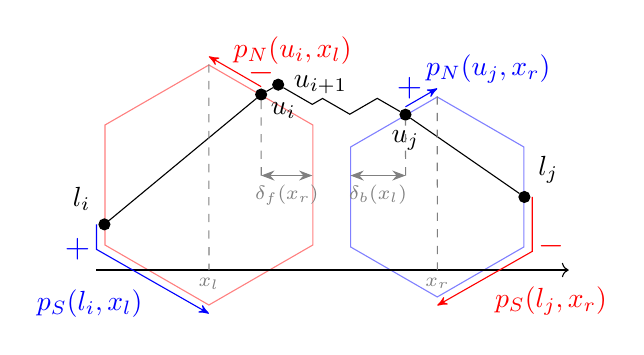
\begin{tikzpicture}%[scale=1, transform shape]
%\clip (1.3,-1) rectangle (8,2.8);

\coordinate (c1) at (2.93,1.18);
\coordinate (c2) at ($(c1)+(2.9,-.15196)$);

\node [draw, color=red!50, shape border rotate=30, minimum size=1.2in, regular polygon, regular polygon sides=6] at (c1) (H1) {};

\node [draw, color=blue!50, shape border rotate=30, minimum size=1in, regular polygon, regular polygon sides=6] at (c2) (H2) {};

 \node at (H1.side 6) [draw,circle,fill,inner sep=1.4pt,label={[label distance=-0.1cm]-85:{$u_i$}}] (ui) {};

 \node at (H1.side 2) [draw,yshift=-0.5cm,circle,fill,inner sep=1.4pt,label={[label distance=0cm]135:$l_i$}] (li) {};

 \node at (H2.side 1) [draw,shift={+(0.15,0.0866cm)},circle,fill,inner sep=1.4pt,label={[label distance=0]-90:{$u_j$}}] (uj) {};

 \node at (H2.side 5) [draw,circle,fill,inner sep=1.4pt,label={[label distance=0cm]45:$l_j$}] (lj) {};

\draw (li) -- (ui);
\draw (lj) -- (uj);

\coordinate (o) at (1.5,0.1);
\coordinate (x) at (7.5,0.1);
\draw [->] (o) -- (x);

\coordinate (N1) at (H1.corner 1);
\coordinate (N1d) at ($(N1)+(-90:4)$);
\coordinate (N1x) at (intersection of o--x and N1--N1d);

\draw [gray, dashed] (N1) -- (N1x);

\node at (N1x) [label={[label distance=-0.15cm]-90:{\color{gray}{{\scriptsize $x_l$}}}}] {};

\coordinate (N2) at (H2.corner 1);
\coordinate (N2d) at ($(N2)+(-90:4)$);
\coordinate (N2x) at (intersection of o--x and N2--N2d);


\draw [gray, dashed] (N2) -- (N2x);

\node at (N2x) [label={[label distance=-0.15cm]-90:{\color{gray}{{\scriptsize $x_r$}}}}] {};

%\coordinate (pr) at ($(pu)+(0:6)$);
%\coordinate (w1) at (H1.side 2);
%\coordinate (w1u) at ($(w1)+(90:6)$);
\coordinate (uid) at ($(ui)+(-90:6)$);
\coordinate (ujd) at ($(uj)+(-90:6)$);
%\coordinate (lu) at ($(l)+(90:6)$);

\coordinate (p1) at (0,1.3);
\coordinate (p2) at (7,1.3);

%\coordinate (z1) at (intersection of w1--w1u and pu--pr);
\coordinate (z3) at (intersection of ui--uid and p1--p2);
\coordinate (z4) at (intersection of N1--N1x and p1--p2);
%\coordinate (z2) at ($(z1)+(z4)-(z3)$);
\coordinate (z5) at (intersection of N2--N2x and p1--p2);
\coordinate (z6) at (intersection of uj--ujd and p1--p2);
%\coordinate (z6) at (intersection of l--lu and pu--pr);

%\draw [gray,<->,{Stealth-Stealth}] ($(z1)+(0,-0.4)$) -- ($(z2)+(0,-0.4)$) node [near start, below] {\scriptsize $\theta_b(x_l)$};

\draw [gray,<->,{Stealth-Stealth}] ($(z6)-(0.7,0)$) -- (z6) node [midway,below] {\scriptsize $\delta_b(x_l)$};

\draw [gray, dashed] (z6) -- (uj);
\draw [gray, dashed] (z3) -- (ui);

\draw [gray,<->,{Stealth-Stealth}] (z3) -- ($(z3)+(0.65,0)$) node [midway,below] {\scriptsize $\delta_f(x_r)$};

\node at (H1.side 2) [yshift=-0.5cm,inner sep=1.4pt,label=-135:{\color{blue}{\large +}}] {};
\node at (H1.side 6) [yshift=-0.05cm,inner sep=1.4pt,label=90:{\color{red}{\large $-$}}] {};
\node at (H1.side 3) [inner sep=1.4pt,label=-135:{\color{blue}{$p_S(l_i,x_l)$}}] {};
\node at (H1.side 6) [xshift=0.4cm, yshift=0.2cm,inner sep=1.4pt,label=90:{\color{red}{$p_N(u_i,x_l)$}}] {};
\node at (H2.side 5) [yshift=-0.3cm,inner sep=1.4pt,label=-45:{\color{red}{\large $-$}}] {};
\node at (H2.side 4) [inner sep=1.4pt,label=-45:{\color{red}{$p_S(l_j,x_r)$}}] {};
\node at (H2.side 1) [xshift=0.2cm,yshift=0.1cm,inner sep=1.4pt,label=90:{\color{blue}{\large $+$}}] {};
\node at (H2.side 1) [xshift=1.2cm,yshift=0.3cm,inner sep=1.4pt,label=90:{\color{blue}{$p_N(u_j,x_r)$}}] {};

\draw ($(li) + (-0.1cm,0)$) -- ($(H1.corner 3) + (-0.1cm,-0.052cm)$) -- ($(H1.corner 4) + (0,-0.1cm)$) [->,>=stealth',blue];
\draw ($(ui) + (0,0.1cm)$) -- ($(H1.corner 1) + (0,0.1cm)$) [->,>=stealth',red];
\draw ($(lj) + (0.1cm,0)$) -- ($(H2.corner 5) + (0.1cm,-0.052cm)$) -- ($(H2.corner 4) + (0,-0.1cm)$) [->,>=stealth',red];
\draw ($(uj) + (0cm,0.1cm)$) -- ($(H2.corner 1) + (0cm,0.1cm)$) [->,>=stealth',blue];

\node at ($(ui)+(30:0.25)$) [draw,circle,fill,inner sep=1.4pt,label={[label distance=0cm]0:{$u_{i+1}$}}] (u2) {};

\coordinate (u3) at ($(u2)+(-30:0.5)$);
\coordinate (u4) at ($(u3)+(30:.15)$);
\coordinate (u5) at ($(u4)+(-30:0.4)$);
\coordinate (x6) at ($(u5)+(30:2)$);
\coordinate (x7) at ($(uj)+(150:2)$);
\coordinate (u6) at (intersection of uj--x7 and u5--x6)
; 
\draw (ui) -- (u2) -- (u3) -- (u4) -- (u5) -- (u6) -- (uj);

%\coordinate (z) at ($(n1)!.5!(n2) + (0.6,0.4)$);
%\node at (z) [label={[label distance=-0.15cm]90:{\color{gray}{{\scriptsize $\theta_b(x_l)=\theta_f(x_r)$}}}}] {};

%\draw [gray,dotted,->,>=Stealth] (n1) -- (z);


%\draw [gray, dashed] (z2) -- ($(z2)+(0,-0.4)$);

\end{tikzpicture}
%%%  \hspace{0.6cm}
%%%  \begin{tikzpicture}[scale=1, transform shape]
%%%  %\clip (1.3,-1) rectangle (8,2.8);
%%%  
%%%  \node [draw, color=red!50, shape border rotate=30, minimum size=1.2in, regular polygon, regular polygon sides=6] at (2.93,1.18) (H1) {};
%%%  
%%%  \coordinate (c1) at (2.93,1.18);
%%%  
%%%  \node at (H1.side 6) [draw,circle,fill,inner sep=1.4pt,label=0:{$u_i$}] (ul) {};
%%%  
%%%   
%%%  \node at (H1.corner 3) [draw,circle,fill,inner sep=1.4pt,label=180:$l_i$] (l) {};
%%%  
%%%  %\draw (l) -- (H1.corner 4) [->,>=stealth',blue,label=-45:{$+$}];
%%%  \draw ($(l) + (0,-0.1cm)$) -- ($(H1.corner 4) + (0,-0.1cm)$) [->,>=stealth',blue,label=45:{$p_S(\ell (x_l),x_l)$}];
%%%  
%%%  \draw ($(ul) + (0,0.1cm)$) -- ($(H1.corner 1) + (0,0.1cm)$) [->,>=stealth',red,label=-45:{$+$}];
%%%  
%%%  
%%%  
%%%  \draw [->] (1,0.1) -- (5,0.1);
%%%  
%%%  \coordinate (N1) at (H1.corner 1);
%%%  
%%%  \node at (N1) [label={[label distance=-0.3cm]135:{\scriptsize $N(x_l)$}}] {};
%%%  
%%%  \draw [gray] (ul) -- (l) -- (N1);
%%%  
%%%  \coordinate (N1x) at (2.93,0.1);
%%%  \draw [gray, dashed] (N1) -- (N1x);
%%%  
%%%  \draw pic [draw=gray, "\color{gray}{\scriptsize $\Theta$}", angle eccentricity=1.25,angle radius=1.05cm] {angle = ul--l--N1};
%%%  
%%%  
%%%  \node at (2.93,0.1) [label={[label distance=-0.15cm]-90:{\color{gray}{$x_l$}}}] {};
%%%  
%%%  \draw [gray,<->,{Stealth-Stealth},label=-90:${\tt r}(x_l)$] ($(N1) + (0,-2)$) -- ($(N1)+(1.32,-2)$) node [midway, below] {\scriptsize ${\tt r}(x)$};
%%%  
%%%  \coordinate (ud) at ($(ul)+(-90:4)$);
%%%  \coordinate (p1) at (0,1.3);
%%%  \coordinate (p2) at (7,1.3);
%%%  \coordinate (z1) at (intersection of ul--ud and p1--p2);
%%%  \coordinate (z2) at (intersection of N1--N1x and p1--p2);
%%%  
%%%  \draw [gray,<->,{Stealth-Stealth},label=90:$\theta_f(x_l)$] (z1) -- (z2) node [very near start, below] {\scriptsize $\theta_f(x_l)$};
%%%  
%%%  \draw [gray,dashed] (ul) -- (z1);
%%%  
%%%  \node at (H1.side 3) [inner sep=1.4pt,label=-135:{\color{blue}{$p_S(l_i,x_l)$}}] {};
%%%  \node at (H1.side 6) [shift={+(-0.15,0.0866cm)},inner sep=1.4pt,label=45:{\color{red}{$p_N(u_i,x_l)$}}] {};
%%%  \end{tikzpicture}
%%%  \center{(a) \hspace{2.6in} (b)}
}

\newcommand{\anotherpathcost}{
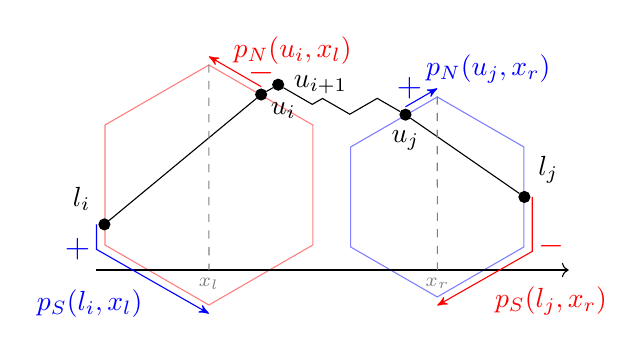
\begin{tikzpicture}%[scale=1, transform shape]
%\clip (1.3,-1) rectangle (8,2.8);

\coordinate (c1) at (2.93,1.18);
\coordinate (c2) at ($(c1)+(2.9,-.15196)$);

\node [draw, color=red!50, shape border rotate=30, minimum size=1.2in, regular polygon, regular polygon sides=6] at (c1) (H1) {};

\node [draw, color=blue!50, shape border rotate=30, minimum size=1in, regular polygon, regular polygon sides=6] at (c2) (H2) {};

 \node at (H1.side 6) [draw,circle,fill,inner sep=1.4pt,label={[label distance=-0.1cm]-85:{$u_i$}}] (ui) {};

 \node at (H1.side 2) [draw,yshift=-0.5cm,circle,fill,inner sep=1.4pt,label={[label distance=0cm]135:$l_i$}] (li) {};

 \node at (H2.side 1) [draw,shift={+(0.15,0.0866cm)},circle,fill,inner sep=1.4pt,label={[label distance=0]-90:{$u_j$}}] (uj) {};

 \node at (H2.side 5) [draw,circle,fill,inner sep=1.4pt,label={[label distance=0cm]45:$l_j$}] (lj) {};

\draw (li) -- (ui);
\draw (lj) -- (uj);

\coordinate (o) at (1.5,0.1);
\coordinate (x) at (7.5,0.1);
\draw [->] (o) -- (x);

\coordinate (N1) at (H1.corner 1);
\coordinate (N1d) at ($(N1)+(-90:4)$);
\coordinate (N1x) at (intersection of o--x and N1--N1d);

\draw [gray, dashed] (N1) -- (N1x);

\node at (N1x) [label={[label distance=-0.15cm]-90:{\color{gray}{{\scriptsize $x_l$}}}}] {};

\coordinate (N2) at (H2.corner 1);
\coordinate (N2d) at ($(N2)+(-90:4)$);
\coordinate (N2x) at (intersection of o--x and N2--N2d);


\draw [gray, dashed] (N2) -- (N2x);

\node at (N2x) [label={[label distance=-0.15cm]-90:{\color{gray}{{\scriptsize $x_r$}}}}] {};

%\coordinate (pr) at ($(pu)+(0:6)$);
%\coordinate (w1) at (H1.side 2);
%\coordinate (w1u) at ($(w1)+(90:6)$);
\coordinate (uid) at ($(ui)+(-90:6)$);
\coordinate (ujd) at ($(uj)+(-90:6)$);
%\coordinate (lu) at ($(l)+(90:6)$);

\coordinate (p1) at (0,1.3);
\coordinate (p2) at (7,1.3);

%\coordinate (z1) at (intersection of w1--w1u and pu--pr);
\coordinate (z3) at (intersection of ui--uid and p1--p2);
\coordinate (z4) at (intersection of N1--N1x and p1--p2);
%\coordinate (z2) at ($(z1)+(z4)-(z3)$);
\coordinate (z5) at (intersection of N2--N2x and p1--p2);
\coordinate (z6) at (intersection of uj--ujd and p1--p2);
%\coordinate (z6) at (intersection of l--lu and pu--pr);

%\draw [gray,<->,{Stealth-Stealth}] ($(z1)+(0,-0.4)$) -- ($(z2)+(0,-0.4)$) node [near start, below] {\scriptsize $\theta_b(x_l)$};

%\draw [gray,<->,{Stealth-Stealth}] ($(z6)-(0.7,0)$) -- (z6) node [midway,below] {\scriptsize $\delta_b(x_l)$};

%\draw [gray, dashed] (z6) -- (uj);
%\draw [gray, dashed] (z3) -- (ui);

%\draw [gray,<->,{Stealth-Stealth}] (z3) -- ($(z3)+(0.65,0)$) node [midway,below] {\scriptsize $\delta_f(x_r)$};

\node at (H1.side 2) [yshift=-0.5cm,inner sep=1.4pt,label=-135:{\color{blue}{\large +}}] {};
\node at (H1.side 6) [yshift=-0.05cm,inner sep=1.4pt,label=90:{\color{red}{\large $-$}}] {};
\node at (H1.side 3) [inner sep=1.4pt,label=-135:{\color{blue}{$p_S(l_i,x_l)$}}] {};
\node at (H1.side 6) [xshift=0.4cm, yshift=0.2cm,inner sep=1.4pt,label=90:{\color{red}{$p_N(u_i,x_l)$}}] {};
\node at (H2.side 5) [yshift=-0.3cm,inner sep=1.4pt,label=-45:{\color{red}{\large $-$}}] {};
\node at (H2.side 4) [inner sep=1.4pt,label=-45:{\color{red}{$p_S(l_j,x_r)$}}] {};
\node at (H2.side 1) [xshift=0.2cm,yshift=0.1cm,inner sep=1.4pt,label=90:{\color{blue}{\large $+$}}] {};
\node at (H2.side 1) [xshift=1.2cm,yshift=0.3cm,inner sep=1.4pt,label=90:{\color{blue}{$p_N(u_j,x_r)$}}] {};

\draw ($(li) + (-0.1cm,0)$) -- ($(H1.corner 3) + (-0.1cm,-0.052cm)$) -- ($(H1.corner 4) + (0,-0.1cm)$) [->,>=stealth',blue];
\draw ($(ui) + (0,0.1cm)$) -- ($(H1.corner 1) + (0,0.1cm)$) [->,>=stealth',red];
\draw ($(lj) + (0.1cm,0)$) -- ($(H2.corner 5) + (0.1cm,-0.052cm)$) -- ($(H2.corner 4) + (0,-0.1cm)$) [->,>=stealth',red];
\draw ($(uj) + (0cm,0.1cm)$) -- ($(H2.corner 1) + (0cm,0.1cm)$) [->,>=stealth',blue];

\node at ($(ui)+(30:0.25)$) [draw,circle,fill,inner sep=1.4pt,label={[label distance=0cm]0:{$u_{i+1}$}}] (u2) {};

\coordinate (u3) at ($(u2)+(-30:0.5)$);
\coordinate (u4) at ($(u3)+(30:.15)$);
\coordinate (u5) at ($(u4)+(-30:0.4)$);
\coordinate (x6) at ($(u5)+(30:2)$);
\coordinate (x7) at ($(uj)+(150:2)$);
\coordinate (u6) at (intersection of uj--x7 and u5--x6)
; 
\draw (ui) -- (u2) -- (u3) -- (u4) -- (u5) -- (u6) -- (uj);

%\coordinate (z) at ($(n1)!.5!(n2) + (0.6,0.4)$);
%\node at (z) [label={[label distance=-0.15cm]90:{\color{gray}{{\scriptsize $\theta_b(x_l)=\theta_f(x_r)$}}}}] {};

%\draw [gray,dotted,->,>=Stealth] (n1) -- (z);


%\draw [gray, dashed] (z2) -- ($(z2)+(0,-0.4)$);

\end{tikzpicture}
}



\newcommand{\mickey}{
\begin{tikzpicture}

\node [draw, color=blue!50, shape border rotate=30, minimum size=2in, regular polygon, regular polygon sides=6] at (2,0) (H) {};



\node [draw, color=red!50, shape border rotate=30, minimum size=1.4641in, regular polygon, regular polygon sides=6,label=-90:{{\color{red!50}{$H_1$}}}] at (1.41,1.02) (L) {};

\node [draw, color=green!50, shape border rotate=30, minimum size=1.4641in, regular polygon, regular polygon sides=6,label=-87:{{\color{green!50}{$H_n$}}}] at (2.59,1.02) (R) {};

\node at (H.corner 1) [draw,circle,fill,inner sep=1.4pt] (u4) {};
\node at (H.corner 3) [draw,circle,fill,inner sep=1.4pt] (l2) {};
\node at (H.corner 4) [draw,circle,fill,inner sep=1.4pt] (l3) {};
\node at (H.corner 5) [draw,circle,fill,inner sep=1.4pt] (l4) {};

\node at (L.corner 3) [draw,circle,fill,inner sep=1.4pt,label=180:$l_1$] (l1) {};
\node at (R.corner 5) [draw,circle,fill,inner sep=1.4pt,label=0:$l_{n-1}$] (l5) {};

\node at (L.corner 2) [draw,circle,fill,inner sep=1.4pt,label=180:$u_1$] (u2) {};
\node at (L.corner 1) [draw,circle,fill,inner sep=1.4pt] (u3) {};
\node at (R.corner 1) [draw,circle,fill,inner sep=1.4pt] (u5) {};
\node at (R.corner 6) [draw,circle,fill,inner sep=1.4pt,label=0:$u_{n-1}$] (u6) {};


\node at (L.corner 4) (LN) {};
\coordinate (LNL) at ($(LN)+(-180:6)$);
\coordinate (m) at (intersection of LN--LNL and u2--l2);

\draw [gray, dashed] (m) -- (LN) node [midway, label={[label distance=-0.1cm]-90:{\color{gray}{$1$}}}] {};

\coordinate (l4L) at ($(l4)+(-180:6)$);
\coordinate (m) at (intersection of l4--l4L and u4--l3);

\draw [gray, dashed] (m) -- (l4) node [near start, label={[label distance=-0.1cm]-90:{\color{gray}{$\frac{\sqrt{3}}{2} + \frac{1}{2}$}}}] {};


\coordinate (h) at (u3);
\coordinate (l) at (l1);

\draw [very thick] (h) -- (l) node [midway, label={[label distance=-0.1cm]180:{\color{gray}{$2$}}}] {};

\foreach \x in {.8,.6,.4,.2}
{
  \node at ($\x*(l1)+(l2)-\x*(l2)$) [draw, fill, inner sep = 1.4pt, circle] (l) {};
  \draw (h) -- (l);
  \node at ($\x*(u3)+(u4)-\x*(u4)$) [draw, fill, inner sep = 1.4pt, circle] (h) {};
  \draw (h) -- (l);
}

\draw (h) -- (l2) -- (u4) -- (l3);


\coordinate (h) at (u5);
\coordinate (l) at (l5);

\draw [very thick] (h) -- (l);

\foreach \x in {.8,.6,.4,.2}
{
  \node at ($\x*(l5)+(l4)-\x*(l4)$) [draw, fill, inner sep = 1.4pt, circle] (l) {};
  \draw (h) -- (l);
  \node at ($\x*(u5)+(u4)-\x*(u4)$) [draw, fill, inner sep = 1.4pt, circle] (h) {};
  \draw (h) -- (l);
}

\draw (h) -- (l4) -- (u4);
\draw [very thick] (u4) -- (u5) -- (u6) -- (l5) -- (l4) -- (l3) -- (l2) node [near end,label={[label distance=0cm]-90:{\color{gray}{$1 + \frac{1}{\sqrt{3}}$}}}] {} -- (u2) -- (u3) node [near start,label={[label distance=0cm]90:{\color{gray}{$\frac{2}{\sqrt{3}}$}}}] {} -- (u4);

%\draw [gray,<->,{Stealth-Stealth}] (z5) -- (z6) node [very near start,label={[label distance=-.17cm]-135:{\color{gray}{{\scriptsize $\theta_b(x_l)$}}}}] {};


\node at ($0.133975*(u2)+(l1)-0.133975*(l1)$) [draw, fill, inner sep = 1.4pt, circle,label=175:$s$] (p) {};
\node at ($0.133975*(u6)+(l5)-0.133975*(l5)$) [draw, fill, inner sep = 1.4pt, circle,label=5:$t$] (q) {};

\draw [dashed] (p) -- (q);

\draw (u2) -- (p) node [midway,label={[label distance=0cm]180:{\color{gray}{$1$}}}] {};
\end{tikzpicture}
}



\begin{document}

%\definecolor{qqwuqq}{rgb}{0.,0.39215686274509803,0.}
%\definecolor{wwzzff}{rgb}{0.4,0.6,1.}

\maketitle

\begin{abstract}
The problem of computing the exact stretch factor (i.e., the tight bound on the
worst case stretch factor) of a Delaunay triangulation is one of the
longstanding open problems in computational geometry. Over the
years, a series of upper and lower bounds on the exact stretch factor have
been obtained but the gap between them is still large. An alternative approach
to solving the problem is to develop techniques for computing the exact stretch
factor of ``easier'' types of Delaunay triangulations, in particular those
defined using regular-polygons instead
of a circle. Tight bounds exist for Delaunay triangulations defined using
an equilateral triangle~\cite{Chew89} and a square~\cite{BGHP15}. In this paper,
we determine the exact stretch factor of Delaunay triangulations defined using
a regular hexagon: It is $2$.

We think that the main contribution of this paper are the two techniques we
have developed to compute tight upper bounds for the stretch factor of
Hexagon-Delaunay triangulations.% The two techniques correspond to the two
%different lower bound construtions which are equivalent to the two tightest
%known lower bound for traditional Delaunay triangulations.  
 %We think that the techniques
%we
%have developed in this paper will prove useful in future work on
%computing the exact stretch factor of classical Delaunay triangulations and
%other plane spanners.
\end{abstract}




%\clearpage
%\setcounter{page}{1}


\section{Introduction}
\label{sec:intro}
\section{Introduction}  \label{sec:introduction}

\newcommand\inexpIntro[3]{#1?(#2,#3).}
\newcommand\rinexpIntro[3]{*#1?(#2,#3).}
\newcommand\outexpIntro[3]{#1!(#2,#3).}
\newcommand\outatomIntro[3]{#1!(#2,#3)}

We propose a fully automated method for proving termination of \(\pi\)-calculus processes.
Although there have been a lot of studies on termination analysis for the \(\pi\)-calculus
and related calculi~\cite{Deng06IC,Demangeon07,SangiorgiTermination,KobayashiHybrid,Yoshida04IC,DBLP:journals/jlp/DemangeonHS10,Venet98SAS}, most of them have been rather theoretical,
and there have been surprisingly little efforts in developing  fully automated termination
verification methods and tools based on them. To our knowledge,
Kobayashi's \typical{}~\cite{TyPiCal,KobayashiHybrid} is the only exception that
can prove termination of \(\pi\)-calculus processes (extended with natural numbers)
fully automatically, but its termination analysis is quite limited (see Section~\ref{sec:relatedwork}).

Our method is based on a reduction to termination analysis for sequential programs:
we translate a \(\pi\)-calculus process \(P\) to a sequential program \(S_P\), so that
if \(S_P\) is terminating, so is \(P\). The reduction allows us to use
powerful, mature methods and tools
for termination analysis of sequential programs~\cite{heizmann2016ultimate,freqterm,DBLP:conf/lics/PodelskiR04,Kuwahara2014Termination,DBLP:journals/cacm/CookPR11}.

The idea of the translation is to convert a chain of communications on replicated input
channels to a chain of recursive function calls of the target sequential program.
Let us consider the following Fibonacci process:
\begin{align*}
    & \rinexpIntro{\fib}{n}{r}
        \ifexp{n<2}{ \soutatom{r}{1} \\ &\quad}
                   { \nuexp{s_1} \nuexp{s_2} (\outatomIntro{\fib}{n-1}{s_1} \PAR \outatomIntro{\fib}{n-2}{s_2} \PAR \sinexp{s_1}{x}\sinexp{s_2}{y}\soutatom{r}{x+y}) \\}
    & \PAR \outatomIntro{\fib}{m}{r}
\end{align*}
Here, the process
$\rinexpIntro{\fib}{n}{r} \ldots$ is a function server that computes the \(n\)-th Fibonacci number
in parallel and returns the result to \(r\),
and $\outatom{\fib}{m}{r}$ sends a request for computing the \(m\)-th Fibonacci number;
those who are not familiar with the syntax of the \(\pi\)-calculus may wish to consult
Section~\ref{sec:targetlanguage} first.
To prove that the process above is terminating for any integer \(m\),
it suffices to show that there is no infinite chain of communications on $\fib$:
\[
    \fib(m,r) \to \fib(m_1,r_1) \to \fib(m_2,r_2) \to \cdots.
\]
We convert the process above to the following program:\footnote{The actual translation
  given later is a little more complex.}
\begin{verbatim}
 let rec fib(n) = if n<2 then () else (fib(n-1) [] fib(n-2)) in
 fib(m)
\end{verbatim}
Here, \texttt{[]} represents the non-deterministic choice.
Note that, although the calculation of Fibonacci numbers is not preserved,
for each chain of communications on \texttt{fib}, there is a corresponding
sequence of recursive calls:
\[
\mathtt{fib}(m) \to \mathtt{fib}(m_1) \to \mathtt{fib}(m_2) \to \cdots.
\]
Thus, the termination of the sequential program above implies the termination of
the original process.
As shown in the example above, (i) each communication on a replicated input channel
is converted to a function call, (ii) each communication on a non-replicated input
channel is just removed (or, in the actual translation, replaced by a call of
a trivial function defined by \(f(\seq{x})=(\,)\)), and (iii) parallel composition
is replaced by a non-deterministic choice.
We formalize the translation outlined above and prove its correctness.

The basic translation sketched above sometimes loses too much information.
For example, consider the following process:
\begin{align*}
    & \rinexpIntro{\pre}{n}{r} \soutatom{r}{n-1} \\
    & \PAR \rinexpIntro{f}{n}{r} \ifexp{n<0}{ \soutatom{r}{1} }
                                       { \nuexp{s} (\outatomIntro{\pre}{n}{s} \PAR \sinexp{s}{x}\outatomIntro{f}{x}{r}) } \\
    & \PAR \outatomIntro{f}{m}{r}
\end{align*}
The translation sketched above would yield:
\begin{verbatim}
  let pred(n) = n-1 in
  let rec f(n) = if n<0 then () else (pred(n) [] f(*)) in
  f(m)
\end{verbatim}
Here, \texttt{*} represents a non-deterministic integer: since we have removed
the input $\sinatom{s}{x}$, we do not have information about the value of \( x \).
As a result, the sequential program above is non-terminating, although the original
process is terminating.
To remedy this problem, we also refine the basic translation above by using a refinement
type system for the \(\pi\)-calculus. Using the refinement type system,
we can infer that the value of \(x\) in the original process is less than \(n\),
so that we can refine the definition of \texttt{f} to:
\begin{verbatim}
 let rec f(n) = ... else (pred(n) [] let x=* in assume(x<n);f(x))
\end{verbatim}
The target program is now terminating, from which
we can deduce that the original process is also terminating.
We have implemented an automated tool based on the refined translation above.

The contributions of this paper are summarized as follows.
\begin{itemize}
\item The formalization of the basic translation from the \(\pi\)-calculus
  (extended with integers) to sequential programs, and a proof of its correctness.
\item The formalization of a refined translation based on a refinement type system.
\item An implementation of the refined translation, including automated refinement type
  inference based on CHC solving, and experiments to evaluate the effectiveness of
  our method.
\end{itemize}

The rest of this paper is structured as follows.
Section~\ref{sec:targetlanguage} introduces the source and target languages
of our translation.
Section~\ref{sec:approach} 
formalizes the basic translation, and proves its correctness.
Section~\ref{sec:refinement} refines the basic translation by using a refinement type system.
Section~\ref{sec:implementation} reports an implementation and experiments.
Section~\ref{sec:relatedwork} discusses related work,
and Section~\ref{sec:conclusion} concludes the paper.


\section{Preliminaries}
\label{sec:prelim}
\section{Preliminaries}\label{chpt:preliminiaries}
In this chapter we will introduce some of the mathematical background and notation needed for this thesis. In particular, we will shortly introduce the differential geometric description of spacetime in Section \ref{sec:spacetime_geometry} and give an introduction to the notion of global hyperbolicity and its connection to Green- and normally-hyperbolic operators in Section \ref{sec:global_hyperbolicity}. In a bit more detail, we will introduce the notion of differential forms and give explicit definitions, also in terms of an index based notation, in Section \ref{sec:differential_forms}. For completeness, in Section \ref{sec:cat-theory}, we present basic definitions of category theory. The reader familiar with these topics can safely skip this chapter and refer to it when interested in the chosen conventions.
%
%
%
%
%%%%%%
%%SPACTIME GEOMETRY
%%%%%
%
%
%
\subsection{Spacetime geometry}\label{sec:spacetime_geometry}
In GR, the universe is mathematically described as a four dimensional \emph{spacetime}, consisting of a smooth, four dimensional manifold \gls{M} (assumed to be Hausdorff, connected, oriented, time-oriented and para-compact) and a Lorentzian metric $g$. We will assume the signature of the Lorentzian metric $g$ to be $(-,+,+,+)$. The Levi-Civita connection on $(\M,g)$ is as usual denoted by \gls{nabla}.
Throughout this thesis, we treat spacetime as fixed, implementing a gravitational background determined classically by Einstein's field equations. Hence, we neglect any back-reaction of the fields on the metric, both in the quantum and the classical case. In that sense, we treat the fields as \emph{test fields}.\par
For the basic mathematical theory regarding Lorentzian manifolds, we refer to the literature: An introduction to the topic with an emphasis on the physical application in GR is for example given in \cite{wald_GR} and \cite{carroll_spacetime-and-gr}.
Here, we will shortly recap the notion of a tangent space and tangent bundle and generalize to the notion of a vector bundle which we will use in the general description of normally hyperbolic operators and differential forms.
In the following, we generalize the setting to an arbitrary smooth manifold $\N$ of dimension $N$ with either Lorentzian or Riemannian metric $k$.\par
%
%
A \emph{tangent vector} $v_x$ at point $x \in \N$ is a linear map $v_x : C^\infty(\N , \IR) \to \IR$ that obeys the Leibniz rule, that is, for $f,g \in C^\infty (\N,\IR)$ it holds $v_x(fg) = f(x)v_x(g) + v_x(f)g(x)$.
We define the \emph{tangent space} \gls{TxN} of $\N$ at $x$ as the real $N$-dimensional vector space of all tangent vectors at point $x$.
The disjoint union of all tangent spaces is called the \emph{tangent bundle} \gls{TN} of $\N$ and is itself a manifold of dimension $2N$. A \emph{vector field} is a map $v: \N \to T\N$ such that $v(x) \in T_x\N$.
The respective dual spaces, that is the space of all linear functionals, the \emph{co-tangent space} and the \emph{co-tangent bundle}, are denoted by \gls{TsxN} and \gls{TsN} respectively.\par
%
For Lorentzian manifolds, we call a tangent vector $v$ at $x \in \N$ \emph{timelike} if $k_{\mu \nu} v^\mu v^\nu < 0$, \emph{spacelike} if $k_{\mu \nu} v^\mu v^\nu > 0$ and \emph{null} (or lightlike) if $k_{\mu \nu} v^\mu v^\nu = 0$. At every point $x \in \N$, we define the set of all \emph{causal}, that is, either timelike or null, tangent vectors in the tangent space at $x$. This set is called the \emph{light cone} at $x$ and it is split up into two distinct parts, one that we call the future light cone, and one that we call the past light cone at $x$. Since we assume the manifold to be time orientable, there exists a smooth vector field $t$ that is timelike at every $x \in \N$. Given this time orientation, we identify the future (past) light cone with the set of tangent vectors $v \in T_x\N$ such that $k_{\mu\nu} v^\mu t^\nu < 0$ (respectively $> 0$). Therefore, a tangent vector $v$ at $x$ is called \emph{future directed} (past directed) if it lies in the future (past) light cone at $x$.\\
Accordingly, a curve $\gamma : I \to \N$ is called timelike (spacelike, null, causal, future or past directed) if its tangent vector $\dot{\gamma}$ is timelike (spacelike, null, causal, future or past directed) at every $x \in \N$.  For every point $x \in \N$ we define the \emph{causal future/past} \gls{causalfuturepast} of $x$ as the set of all points $q \in \N$ that can be reached by a future directed causal curve originating in $x$. For any subset $S \in \N$ we define $J^\pm (S) = \bigcup_{x \in S} J^\pm(x)$ and $J(S) = J^+(S) \cup J^- (S)$. Finally, the future/past domain of dependence $\gls{futurepastdomainofdependence}$ of a set $S \subset \N$ is the set of all points $x \in \N$ such that every inextendible causal curve through $x$ intersects $S$. The \emph{domain of dependence} \gls{domainofdependence} of $S$ is the union of the future and past domain of dependence of the set $S$.
For more details on the causal structure of spacetime we refer to for example \cite[Chapter 8]{wald_GR}.\par
%
%
%
The notion of tangent bundles can be generalized to the notion of a vector bundle. Instead of ``attaching'' the vector spaces $T_x \N$ to every point $x$ of the manifold, we allow for the occurrence of arbitrary vector spaces, called the fibres of the vector bundle. A vector bundle then consists of the base manifold, in our case $\N$, the total space and a map $\pi$ from the total space to the base manifold, that can be locally trivialized. At each point of the base manifold, the pre-image of $\pi$ is the fibre of the vector bundle. To be precise we define, following \cite{rudolph_schmidt}:
\begin{definition}[Vector bundle]
	A smooth \emph{vector bundle} over $\N$ is a tuple $\gls{vectorbundle} = (E,\N, \pi)$, where $E$ is a smooth manifold and $\pi : E \to \N$ is a smooth surjective map satisfying:
	\begin{enumerate}
		\item For every $x \in \N$, $\pi^{-1}(x)$ is a vector space, called the fibre of the bundle at point $x$.
		\item There exists a finite dimensional vector space $F$, an open covering $\left\{ U_\alpha\right\}_\alpha$ of $\N$ and a family of diffeomorphisms $\chi_\alpha : \pi^{-1}(U_\alpha) \to U_\alpha \times F$ such that for all $\alpha$ it holds $\chi_\alpha \comp \text{pr}_1 =  \restr{\pi}{\pi^{-1}(U_\alpha)}$ and for every $x \in \N$ the map $\text{pr}_2 \comp \restr{\chi_\alpha}{\pi^{-1}(x)} : \pi^{-1}(x) \to F$ is linear.
	\end{enumerate}
\end{definition}
Here, the maps $\text{pr}_1$ and $\text{pr}_2$ denote the projection onto the first respectively second component of an element in $U_\alpha \times F$. The properties graphically mean that \emph{locally}, the vector bundle ``looks like" the product of the base manifold with the fibre. The tuples $(U_\alpha, \chi_\alpha)$ are called \emph{local trivializations} of the vector bundle. Like for vector spaces, we can define the sum and product of vector bundles, by using the according vector space definitions on the fibres of the bundle.\par
Let $\mathfrak{X}, \mathfrak{Y}$ be vector bundles over $\N$ with fibres $X_x$ and $Y_x$ at $x \in \N$. We denote by \gls{whitneysum} the \emph{Whitney sum} of the two vector bundles - the vector bundle over $\N$ whose fibres are given by the direct sum $X_x \oplus Y_x$. Similarly, one obtains the local trivializations of the Whitney sum from the trivializations of $\mathfrak{X}, \mathfrak{Y}$ and direct sums.\par
Accordingly, let $\mathfrak{X}, \mathfrak{Y}$ be vector bundles over $\N$ and $\widetilde{\N}$, with fibres $X_x$ and $Y_{\tilde{x}}$ at $x \in \N$, $\tilde{x} \in \widetilde{\N}$ respectively. We denote by \gls{outerproductbundle} the \emph{outer product} of the two vector bundles - the vector bundle over $\N \times \widetilde{\N}$ whose fibres are given by the tensor products $X_x \otimes Y_x$. Similarly, one obtains the local trivializations of the outer product from the trivializations of $\mathfrak{X}, \mathfrak{Y}$ and tensor products. \par
%
Finally, we generalize the notion of vector fields:
\begin{definition}[Sections of vector bundles]
Let $\mathfrak{X}=(E,\N,\pi)$ be a vector bundle with fibres $X_x=\pi^{-1}(x)$ at $x \in \N$. A \emph{smooth section} of the vector bundle is a smooth map $\gamma : \N \to E$ such that $\gamma(x) \in X_x$ for all $x \in \N$. The \emph{vector space of smooth sections} of $\mathfrak{X}$ is denoted by \gls{gammax}, the one with compactly supported sections is as usual denoted by \gls{gammaxzero}.
\end{definition}
In this language, a vector field $v$ is just a smooth section of the tangent bundle of a manifold, $v \in \Gamma(T\N)$. One may therefore identify the physical notion of fields with smooth sections of vector bundles. This point of view will be used to define the notion of differential forms in Section \ref{sec:differential_forms}.\par
In this thesis, we usually are interested in complex valued functions (or sections in general). Therefore, we view all occurring vector bundles as complex, in the sense that we take two distinct copies of the vector bundle, one representing the real, one the imaginary part of the bundle. A section of that complex vector bundle is just a pair of two sections of the real vector bundle under consideration. From now, if not specified explicitly, we will view all vector bundles, including the tangent bundle $T\N$, as complex vector bundles. Accordingly, smooth sections of those bundles will in general be complex valued.
%
%
%
%
%
%
%
%
%%%%%%%
%%PARTIAL DIFFERENTIAL OPERATORS AND GLOBAL HYPERBOLICITY
%%%%%%%
%
%
%
\subsection{Partial differential operators and global hyperbolicity}\label{sec:global_hyperbolicity}
When dealing with field theories, whether classical or quantum, one is, of course, interested in the dynamics of the fields. These are usually described by some partial differential equation, often of second order. In the following, we give a short introduction to the theory of certain partial differential operators acting on smooth sections of a vector bundle over the spacetime $(\M,g)$.\par
%
As we have seen, these smooth sections are generalizations of the notion of a field.  In the following, let $\mathfrak{X}$ denote a vector bundle over the manifold $\M$ and let $P: \Gamma(\mathfrak{X}) \to \Gamma(\mathfrak{X})$ be a partial differential operator acting on smooth sections of the bundle. As in the case of flat spacetime, we are interested in basic questions regarding the differential equation $Pf = j$, for example: Can we formulate a (globally) well posed initial value problem? Does the differential equation possess (unique) solutions? To answer these questions, we will now restrict to the case where $P$ is linear and of second order, as it is often the case in physical applications. One can show that for a certain class of such operators, namely normally hyperbolic partial differential operators of second order, we can rigorously treat these questions.\par
Choosing local coordinates $x=(x_\mu)$ on $\M$ and a local trivialization of $\mathfrak{X}$, a linear partial differential operator of second order is called \emph{normally hyperbolic} if it takes the form
\begin{align}
	P = - \sum_{\mu,\nu} g^{\mu \nu} \partial_\mu \partial_\nu + \sum_{\alpha} A_\alpha (x) \partial_\alpha + B(x) \formspace,
\end{align}
where $A_\alpha$ and $B$ are matrix-valued coefficients depending smoothly on the coordinate $x$ (see. \cite[Chapter 1.5]{baer_ginoux_pfaeffle}). One can also formulate a coordinate independent definition in terms of the principal symbol, which we will not present here (see for example \cite[Section 1.5]{baer_ginoux_pfaeffle} ). \par
%
Normally hyperbolic operators possess unique fundamental solutions (see for example the fundamental solutions to the wave operator as noted in Lemma \ref{lem:fundamental_solution_wave_operator}). These fundamental solutions fulfill certain physically important properties, such as a finite propagation speed smaller than the speed of light. Furthermore, specifying the initial data on some space-like hypersurface $X \in  \M$ specifies a unique solution on the domain of dependence $D(X)$ of $X$. Due to these properties, one often calls normally hyperbolic operators just \emph{wave operators}. But to state a \emph{globally} well posed initial value problem for a wave equation, we need to restrict the class of spacetimes $\M$ under consideration to those that possess space-like hypersurfaces $X$ whose domain of dependence is all of the spacetime, $D(X) = \M$. This leads to the notion of \emph{globally hyperbolic} spacetimes:
\begin{definition}[Global Hyperbolicity]
	A spacetime $\M$ is called \emph{globally hyperbolic} if there exists a Cauchy surface $\gls{sigma}$ in $\M$.
\end{definition}
\noindent Here, a Cauchy surface is a space-like hypersurface $\Sigma \subset \M$ such that every inextendible causal curve $\gamma$ intersects $\Sigma$ exactly once. One can show that Cauchy surfaces fulfill the desired property mentioned above, that is,  $D(\Sigma) = \M$. Furthermore, one can show that any globally hyperbolic spacetime $\M$ is foliated by a one-parameter family $\left\{ \Sigma_t \right\}_t$ of Cauchy surfaces (see for example \cite[Theorem 8.3.14]{wald_GR}). \par
In physical applications, one often finds the dynamics of a theory to be described by wave operators. Most prominently, the Klein-Gordon operator $(\square + m^2)$ acting on scalar fields, or its generalization, the wave operator acting on differential forms introduced in Section \ref{sec:differential_forms}, is normally hyperbolic. But there are also important physical field theories that are not described by wave operators, such as the Proca field treated in this thesis. It turns out that the Proca operator (see Definition \ref{def:proca_operator}) is a so called \emph{Green-hyperbolic} operator. These are again partial differential operators $P$ of second order acting on smooth sections of some vector bundle, such that $P$ (and its dual $P'$) posses fundamental solutions. Obviously, normally hyperbolic operators are Green-hyperbolic, but the opposite is not true. One can generalize some results obtained by studying normally hyperbolic operators to Green-hyperbolic operators. An introduction to this topic is given in \cite{baer_green-hyperbolic}, where it is also shown that the Proca operator is Green-hyperbolic but not normally hyperbolic.\par
For our application, the notion of Green-hyperbolicity is not of vast importance, but it is worth mentioning that there exists a more detailed mathematical background on the treatment of such operators.
A very detailed description of normally hyperbolic operators on Lorentzian manifolds, including proofs of the above statements regarding the initial value problem and the existence of fundamental solutions, is given in \cite{baer_ginoux_pfaeffle}, also with an overview of quantization. A shorter introduction to the topic is for example treated in \cite{baer-ginoux_classical-and-quantum-fields}, also with a description of quantization.
%
%
%
%
%
%
%%%
%
%
%
%%
%%%%%%%%%
%%%DIFFERENTIAL FORMS
%%%%%%%%
%
%
%
\subsection{Differential forms}\label{sec:differential_forms}
%
%
Differential forms provide an elegant, coordinate independent description of calculus on smooth manifolds. In particular, they generalize the notion of line- and volume-integrals that are known from analysis. Differential forms play a remarkable role in physics, as one can argue that they indeed describe fundamental physical entities. As an example, instead of viewing a classical force as a vector, one can think of it, more closely related to experiments, as a differential one-form that assigns a scalar to a tangent vector of a curve. This scalar is the (infinitesimal) work associated with the force along the curve. Also, differential forms allow for an elegant geometric description of field theories, for example the Maxwell and Proca field theories that we encounter in this thesis. In Maxwell's classical theory of electromagnetism, instead of viewing the electric and magnetic field (which are conceptually just forces) as the fundamental physical entities, one introduces the \emph{vector potential}, a one-form, consisting of the scalar electric potential and the vector potential associated with the magnet field. Experiments like the Aharonov-Bohm experiment allow for an interpretation of the vector potential as the fundamental physical object, rather than the associated electromagnetic field. \\
Even more fundamentally, the two main theories of physics, General Relativity and the Standard Model of particle physics, are field theories. They are deeply connected to a geometric interpretation and can be elegantly described using differential forms. \par
%
%
Despite of all this, differential forms are usually not part of the standard curriculum of physicists. We shall therefore introduce the basic aspects and definitions regarding differential forms that are used in this thesis. For a more detailed introduction we refer to the literature: For example \cite[Chapter 2 and 4]{rudolph_schmidt} or \cite[Appendix B]{wald_GR} provide introductions to the topic.\par
%
%
In the following, let $\N$ denote a smooth $N$-dimensional manifold, assumed to be Hausdorff, connected, oriented and para-compact, with either Lorentzian or Riemannian metric $k$ and Levi-Civita connection $\nabla$. For a Lorentzian manifold we use the sign convention $(-,+,\dots,+)$ of the metric $k$. The number of negative eigenvalues of $k$ is denoted by $s$, so $s=0$ for a Riemannian manifold and, in our convention, $s=1$ for a Lorentzian manifold.
Later, we will specify to a four dimensional (globally hyperbolic) spacetime consisting of a four dimensional manifold $\M$ with Lorentzian metric $g$ and Cauchy surface $\Sigma$ with induced Riemannian metric $h$.
%
We define:
\begin{definition}[Differential form]
	Let $p\in \{0,1,\dots,N\}$. A \emph{differential form} $\omega$ of degree $p$, or $p$-form for short, on the manifold $\N$ is an anti-symmetric tensor field of rank $(0,p)$. That is, at every point $x \in \N$, $\omega_x$ is an anti-symmetric multi-linear map
	\begin{align}
	\omega_x : \underbrace{T_x \N \times T_x \N \times \cdots \times T_x \N}_{p\text{-times}} \to \IR \formspace.
	\end{align}
	We denote the vector space\footnote{Naturally, addition and scalar multiplication are defined point-wise.} of $p$-forms on $\N$ by $\gls{omegap}$, the space with compactly supported ones by \gls{omegapz}.
\end{definition}
As an example, a zero-form $f \in \Omega^0(\N)$ is just a $C^\infty$-function from $\N$ to $\IR$, hence we can identify $\Omega^0(\N) = C^\infty (\N, \IR)$. A one-form $A \in \Omega^1(\N)$ is nothing more than a co-vector field and in a physical context usually denoted in local coordinates by $A_\mu$. Note, that alternatively one can directly define a $p$-form as a smooth section of the $p$-th exterior product of the co-tangent bundle and hence identify $\Omega^p(\N) = \Gamma \big( \largewedge^k T^*\N\big)$. As mentioned in Section \ref{sec:spacetime_geometry}, we view the tangent bundle as a complex bundle. Therefore, the sections of that bundle will be complex valued functionals. In that fashion, we will usually view the spaces $\Omega^p(\N)$ as complex valued differential forms.\par
%
Next we define the basic operations, besides addition and scalar multiplication, that one can perform on differential forms.
%
\begin{definition}[Exterior product]
	Let $A \in \Omega^p(\N)$ be a $p$-form and  $B\in \Omega^q(\N)$ a $q$-form on $\N$. \\
	The \emph{exterior product} $\gls{wedge}:\Omega^p(\N) \times \Omega^q(\N) \to \Omega^{p+q} (\N)$ is defined by
	\begin{align}
	(A \wedge B)_{\mu_1\dots\mu_p \nu_1\dots\nu_q} = \frac{(p+q)!}{p!q!}\, A_{[\mu_1 \dots \mu_p} B_{\nu_1\dots\nu_q]} \formspace,
	\end{align}
	where the anti-symmetrization of a tensor $T$ is given through
	\begin{align}
	T_{[\mu_1\dots\mu_p]} = \frac{1}{p!} \sum\limits_{\sigma\in S_N }\textrm{sgn}(\sigma) T_{\sigma(\mu_1)\dots\sigma(\mu_p)} \formspace.
	\end{align}
\end{definition}
Here, $S_N$ denotes the symmetric group\footnote{Usually the symmetric group is defined as the set of permutations of $\{1,2,\dots,N\}$ but we chose the index to run over $\{0,1,\dots,N-1\}$, identifying the time component with zero rather then one.} of degree $N$, consisting of permutations of the set $\{0,1,\dots,N-1\}$.
With this notion of multiplication, point-wise addition and scalar multiplication, the space $\gls{omega} \coloneqq \bigoplus_{p = 0}^\infty \Omega^p(\N) = \bigoplus_{p = 0}^N \Omega^p(\N)$ becomes an algebra, usually called the Grassmann- or \emph{exterior algebra} of differential forms on $\N$. We have used that obviously $\Omega^k(\N) =0$ for $k >N$ due to the anti-symmetrization.\par
Furthermore, we find a notion of how to \emph{pullback} differential forms on manifolds to another manifold, for example the pullback of a differential form on the spacetime $\M$ to differential forms on its Cauchy surface $\Sigma$. Given a $C^\infty$-map $\psi: \widetilde{\N} \to \N$, where $\N, \widetilde{\N}$ are manifolds, we can naturally define the pullback of a function $f \in \Omega^0(\N)$ to a function $(\psi^* f) \in \Omega^0(\widetilde{\N})$ by composing $f$ with $\psi$:
\begin{align}
\psi^* f \coloneqq f \comp \psi \formspace.
\end{align}
\newpage
With the pullback of functions defined, we can define how to \emph{push forward}, or carry along, vector fields on $\widetilde{\N}$ to vector fields on $\N$: Let $f\in \Omega^0(\N)$ and $\tilde{v} \in \Gamma(T\widetilde{\N})$ and $\tilde{x} \in \widetilde{\N}$. Then
\begin{align}
(\psi_* \tilde{v})_{\psi(\tilde{x})} (f) \coloneqq \tilde{v}_{\tilde{x}}(\psi^* f)
\end{align}
defines the vector field $(\psi_* v) \in \Gamma(T\N)$. With these basic operations at hand, we can generalize to define the pullback of differential forms:
\begin{definition}[Pullback]\label{def:pullback}
	Let $\N, \widetilde{\N}$ be manifolds of dimension $N,\widetilde{N}$ respectively, and let $\psi: \widetilde{\N} \to \N$ be a smooth map. Then, $\psi$ defines an algebra homomorphism $\psi^* : \Omega(\N) \to  \Omega(\widetilde{\N})$,
	called the \emph{pullback} of differential forms. For $\omega \in \Omega^p(\N)$, $\tilde{x} \in \widetilde{\N}$ and $\tilde{v}_i \in T_x \widetilde{\N}$, $i=1,2,\dots,p$, it is defined by
	\begin{align}
	\left( \psi^* \omega \right)_{\tilde{x}}  (\tilde{v}_1,\tilde{v}_2,\dots,\tilde{v}_p) \coloneqq \omega_{\psi(\tilde{x})} (\psi_* \tilde{v}_1, \dots , \psi_* \tilde{v}_p) \formspace.
	\end{align}
\end{definition}
%
%
%
%
On the exterior algebra we find a duality, provided by the Hodge operator:
\begin{definition}[Hodge dual]
	The hodge star operator $\gls{hodge}: \Omega^p(\N) \to \Omega^{N-p}(\N)$ is defined through
	\begin{align}
	B \wedge *A = \frac{1}{p!} B^{\mu_1\dots\mu_p}A_{\mu_1\dots\mu_p} \dvolk \formspace,
	\end{align}
	which yields the coordinate representation
	\begin{align}
	(*A)_{\mu_{p+1}\dots\mu_N} = \frac{\detk}{p!} \, \epsilon_{\mu_1\dots\mu_N} A^{\mu_1\dots\mu_p} \formspace.
	\end{align}
\end{definition}
Here, \gls{levicivita} denotes the fully antisymmetric tensor of rank $N$ (Levi-Civita symbol) satisfying $\epsilon_{12,\dots,N} =1$ and the \emph{volume element} \gls{dvolk} is defined by
\begin{align}
\left( \gls{dvolk} \right)_{\alpha_1\dots\alpha_N} = \detk \, \epsilon_{\alpha_1\dots\alpha_N} \formspace.
\end{align}
In a sense, the volume element describes how the curvature of the manifold deforms a unit volume.
The duality follows from the important property of the Hodge operator as stated in the following lemma:
\begin{lemma}
	Let $*$ denote the Hodge star operator on the exterior algebra $\Omega(\N) $. It holds that
	\begin{align}
	** = (-1)^{s+p(N-p)} \, \mathbbm{1} \formspace,
	\end{align}
	which is trivially equivalent to $*^{-1} = (-1)^{s+p(N-p)} \, *$.
\end{lemma}
\begin{proof}
	Let $A \in \Omega^p(\N)$ be a $p$-form on $\N$. Then:
	\begin{align}
	(*{*A})_{\mu_1 \dots \mu_p}
	&= \frac{\detk \, \detk}{p! \, (N-p)!} \; \epsilon_{\alpha_{p+1}\dots\alpha_N \mu_1 \dots \mu_p}\;\epsilon^{\alpha_{1}\dots\alpha_N}\;A_{\alpha_1\dots\alpha_p} \notag\\
	&= (-1)^{p(N-p)} \frac{\detk \, \detk}{p! \, (N-p)!} \; \epsilon_{\alpha_{p+1}\dots\alpha_N \mu_1 \dots \mu_p}\;\epsilon^{\alpha_{p+1}\dots\alpha_{N}\alpha_1\dots\alpha_p}\;A_{\alpha_1\dots\alpha_p}  \notag\\
	&= (-1)^{s+p(N-p)} \delta\indices{^{[\alpha_{1}}_{\mu_{1}}}\, \dots \, \delta\indices{^{\alpha_p ] }_{\mu_p}} \;A_{\alpha_1\dots\alpha_p} \notag\\
	&=  (-1)^{s+p(N-p)}\;A_{\mu_1\dots\mu_p} \formspace
	\end{align}
	We have used Lemma \ref{lem:epsilon_contraction} and, in the last step, that the anti-symmetrization is absorbed by contraction because $A$ is antisymmetric.
\end{proof}
%
%
%
%
%
Furthermore, we can equip the exterior algebra with a differentiable structure, introducing the notion of the exterior derivative.
\begin{definition}[Exterior derivative]
	The \emph{exterior derivative} $\gls{d}:\Omega^p(\N) \to \Omega^{p+1} (\N)$ is defined by the following properties:
	\begin{enumerate}
		\item $d$ is linear
		\item $d$ obeys a graded Leibniz rule: Let $A \in \Omega^p(\N)$ and  $B\in \Omega^q(\N)$, then
		\begin{align}
		d(A \wedge B) = dA \wedge B + (-1)^p \, A \wedge dB
		\end{align}
		\item $d$ is nilpotent, that is,  $d^2 = 0$.
	\end{enumerate}
	In local coordinates, this is equivalent to the representation
	\begin{align}
	(dA)_{\mu \alpha_1\dots\alpha_p} = (p+1)\, \nabla_{[\mu}A_{\alpha_1\dots\alpha_p]} \formspace.
	\end{align}
\end{definition}
An important property of the exterior derivative is that it commutes (or rather intertwines its action) with pullbacks (see \cite[Proposition 4.1.7]{rudolph_schmidt}).
A $p$-form $\omega \in \Omega^p(\N)$ is called \emph{exact} if there is a $(p-1)$-form $\alpha \in \Omega^{p-1}(\N)$ such that $\omega = d\alpha$. We call $\omega$ \emph{closed} if $d \omega =0$. Accordingly, the space of closed $p$-forms is denoted by \gls{omegapd}, the space of exact ones by \gls{domegap}. As usual, the ones with compact support are denoted by a subscript zero. Note, that every exact form is closed, using that $d$ is by definition nilpotent, but the reverse is in general not true. It does hold, however, on certain manifolds with trivial topology, such as Minkowski spacetime. This is expressed in the so called Poincar\'e-Lemma (see for example \cite[Chapter 4]{bott_tu}) based on the study of de Rham cohomology.\par
%
Moreover, $N$-forms can naturally be integrated. Using local coordinates and a partition of unity, we define the integral of $N$-forms via the well known integration on $\IR^N$:
\begin{definition}[Integration on manifolds]
	Let $\left\{U_\alpha, \psi_\alpha\right\}_\alpha$ be an atlas of the manifold $\N$ and $\left\{\chi_\alpha\right\}_\alpha$ a partition of unity subordinate to the locally finite open cover $\left\{U_\alpha\right\}_\alpha$. Let $x^\mu_{(\alpha)}$ be a coordinate basis of $\psi$ on $U_\alpha$. For any $N$-form $\omega \in \Omega^N_0(\M)$ we define the integral
	\begin{align}
	\int\limits_{\N} \omega &\coloneqq \sum_{\alpha} \int\limits_{\psi_\alpha (U_\alpha)} w(x_{(\alpha)}^0,\dots,x_{(\alpha)}^1)\; dx_{(\alpha)}^0 \cdots dx_{(\alpha)}^{N-1} \formspace,
	\end{align}
	where $w$ are the components of $\omega$ in the coordinates $x_{(\alpha)}^\mu$, that is $\omega = w dx_{(\alpha)}^0 \wedge \cdots \wedge dx_{(\alpha)}^{N-1}$.
	This definition is independent of the choice of the atlas and the partition of unity (see \cite[Proposition 3.3]{bott_tu}).
\end{definition}
With integration at our disposal, we present an important theorem regarding the integration of exact differential forms:
\begin{theorem}[Stoke's Theorem]\label{thm:stokes}
	Let $\N$ be an oriented manifold of dimension $N$ and let its boundary $\partial \N$ be endowed with the induced orientation. Let $\gls{inclusionmap} : \partial \N \hookrightarrow \N$ be the inclusion operator.
	Let $\omega \in \Omega^{N-1}_0(\N)$ be a compactly supported $(N-1)$-form on $\N$. Then it holds
	\begin{align}
	\int\limits_\N d\omega = \int\limits_{\partial \N} i^*\omega \formspace.
	\end{align}
\end{theorem}
\begin{proof}
	A proof is given in most of the introductory literature on differential geometry (see for example \cite[Chapter 17, Theorem 2.1]{lang}).
	Note that one can equivalently formulate Stoke's theorem on a \emph{compact} manifold but for {arbitrary} (that is, in general not compactly supported) $(N-1)$-forms on the manifold (see for example \cite[Theorem 4.2.14]{rudolph_schmidt}). This will be of importance in later calculations.
\end{proof}
%
Furthermore, we can define a bilinear map on $\Omega^p(\N)$ using the integration of $N$-forms:
\begin{definition}
	Let $A,B \in \Omega^p(\N)$ such that their supports have a compact intersection. Define the bilinear map $\gls{innerprod} : \Omega^p(\N) \times \Omega^p(\N) \to \IC$ by
	\begin{align}
	\langle A, B \rangle_\N \coloneqq  \int_{\N } A \wedge * B = \int_{\N } A_{\mu_1 \dots \mu_p}B^{\mu_1 \dots \mu_p}\,\dvolk \formspace.
	\end{align}
\end{definition}
Since by definition $A \wedge * B$ is a compactly supported $N$-form, this is well defined. We may sometimes refer to $\langle \cdot , \cdot \rangle_\N$ as an inner product for simplicity, even though it is not positive definite.
%
%
%
%
%
Using the exterior derivative, we define the interior or co-derivative:
\begin{definition}[Interior derivative]
	The \emph{interior derivative} $\gls{delta} : \Omega^p(\N) \to \Omega^{p-1}(\N)$ is defined by
	\begin{align}
	\delta \coloneqq (-1)^{s+1+N(p-1)}\, {*{d*}} \formspace.
	\end{align}
	From the defining properties of $d$ and $*$ it follows $\delta^2 =0$.
\end{definition}
Here, $s$ again denotes the number of negative eigenvalues of the metric $k$ of $\N$. In accordance with our nomenclature, we call a $p$-form $\omega$ co-exact if there exists a $\alpha \in \Omega^{p+1}(\N)$ such that $\omega = \delta \alpha$ and co-closed if $\delta \omega = 0$. Accordingly, the spaces of co-closed and co-exact $p$-forms are denoted by \gls{omegapdelta} and \gls{deltaomegap} respectively.\par
Using the exterior and interior derivative we define the partial differential operator:
\begin{definition}[D'Alembert Operator]
	The d'Alembert (or Laplace - de Rham) operator $\gls{dalembert}: \Omega^p(\N) \to \Omega^{p}(\N)$ is defined by
	\begin{align}
	\square \coloneqq \delta d +d \delta \formspace.
	\end{align}
\end{definition}
By definition of the exterior and interior derivative, it is easy to show that $\square$ commutes with both $d$ and $\delta$:
\begin{align}
\square d &= (\delta d + d \delta )d \notag \\
&= d \delta d \notag \\
&= d (\delta d + d \delta) \formspace,
\end{align}
and analogously for $\delta$.
The d'Alembert operator, and its generalization to $(\square + m^2)$ for some constant $m > 0$, are important examples for a normally hyperbolic differential operators (see Section \ref{sec:global_hyperbolicity}) and we may therefore sometimes just refer to them as \emph{wave operators}.\par
The sign convention in the definition of the exterior derivative is chosen such that on any Lorentzian or Riemannian manifold the interior derivative is formally adjoint to the exterior derivative, that is,  for $A \in \Omega^{p}(\N)$ and $B \in \Omega^{p+1}(\N)$ it holds that
\begin{align}
\langle dA , B \rangle_{\N} = \langle A , \delta B \rangle_\N \formspace,
\end{align}
which leads to a representation in local coordinates of the Manifold given by:
\begin{align}
(\delta A)_{\mu_2\dots\mu_p} = - \nabla^{\mu_1}A_{\mu_1\dots\mu_p} \formspace.
\end{align}
To see that this is consistent, let $A \in \Omega^{p-1}(\N)$ and $B \in \Omega^{p}(\N)$ such that their supports have compact intersection.
We obtain, using Stoke's Theorem \ref{thm:stokes}:
\begin{align}
0 &= \int \limits_{\partial \N} i^* (A \wedge *B) \notag\\
&= \int \limits_{\N} d(A \wedge *B)  \notag\\
&= \int \limits_{\N} dA \wedge *B + (-1)^{p-1} A \wedge d{*B} \notag\\
&= \int \limits_{\N} dA \wedge *B + (-1)^{p-1} A \wedge *{*^{-1}}\underbrace{d{*B}}_{\textrm{is a } (N-p+1) \textrm{ form.}} \notag\\
&= \int \limits_{\N} dA \wedge *B + (-1)^{p-1}(-1)^{s+(N-p+1)(N-N+p-1)} A \wedge *{*d{*B}} \notag\\
&= \int \limits_{\N} dA \wedge *B + (-1)^{p+(1-p)(p-1)} A \wedge *\delta B \formspace.
\end{align}
It can easily be proven by induction that $\big(p+(1-p)(p-1)\big)$ is odd for any $p \in \IN$, which yields the result
\begin{align}
\langle dA , B \rangle_{\N} = \langle A , \delta B \rangle_\N \formspace.
\end{align}
The definitions stated above thus fulfill the requirement of formal adjointness of the exterior and interior derivate on an arbitrary Lorentzian or Riemannian manifold $\N$.
In local coordinates we use a partial integration to obtain
\begin{align}
\langle dA , B \rangle_\N &= \int \limits_{\N} dA \wedge * B \notag\\
%&= \int \limits_{\N} \frac{1}{p!} (dA)^{\alpha_1\dots\alpha_p}\,B_{\alpha_1 \dots \alpha_p} \, \dvolk \notag\\
&= \int \limits_{\N}  \frac{p}{p!} \nabla^{[\alpha_1}A^{\alpha_2\dots\alpha_p]}\,B_{\alpha_1 \dots \alpha_p} \, \dvolk \notag\\
&= \int \limits_{\N}  \frac{1}{(p-1)!} \nabla^{\alpha_1}A^{\alpha_2\dots\alpha_p}\,B_{\alpha_1 \dots \alpha_p} \, \dvolk \notag\\
&= - \int \limits_{\N}  \frac{1}{(p-1)!} A^{\alpha_2\dots\alpha_p}\, \nabla^{\alpha_1}B_{\alpha_1 \dots \alpha_p} \, \dvolk \notag\\
&= \langle A, \delta B \rangle_\N \formspace,
\end{align}
which yields
\begin{align}
-\nabla^{\alpha_1}B_{\alpha_1 \dots \alpha p} = (\delta B)_{\alpha_2 \dots \alpha_p}\formspace.
\end{align}
On the four dimensional spacetime $(\M,g)$ the definitions of the Hodge star operator and the interior derivative simplify, such that
\begin{align}
*_{(\M)}*_{(\M)} &= (-1)^{p+1} \mathbbm{1} \\
\delta_{(\M)} &= *_{(\M)}{d_{(\M)}*_{(\M)}} \formspace ,
\end{align}
holds on the spacetime $(\M,g)$ and
\begin{align}
*_{(\Sigma)}*_{(\Sigma)} &= \mathbbm{1} \\
\delta_{(\Sigma)} &= (-1)^p *_{(\Sigma)}{d_{(\Sigma)}*_{(\Sigma)}}
\end{align}
holds on  $(\Sigma,h)$. In the following we will drop the subscript ${(\M)}$, since we will perform all the calculations on a four dimensional spacetime, except when explicitly noted (for example with a subscript $(\Sigma)$).
%
%
%
%
%
%
%
%
%%%%%%
%%CATEGORY THEORY
%%%%%%
\subsection{Category theory}\label{sec:cat-theory}
The description of Quantum Field Theory on Curved Spacetimes (QFTCS) in the framework of \name{Brunetti}, \name{Fredenhagen} and \name{Verch} \cite{Brunetti_Fredenhagen_Verch} is based on category theory. In this thesis, we will not go into detail on those categorical aspects, however we will need some basic definitions to formulate the theory rigorously, that is namely the notion of a category and that of covariant functors, since, in the used framework, the generally covariant QFTCS is a functor.\par
Here, we present definitions given in \cite[Appendix A.1]{baer_ginoux_pfaeffle} and refer to the appropriate literature for details. We define:
\begin{definition}[Category]
	A \emph{category} $\mathsf{Cat}$ consists of the following:
	\begin{enumerate}
		\item a class $\mathsf{Obj}_\mathsf{Cat}$ whose members are called \emph{objects},
		\item a set $\mathsf{Mor}_\mathsf{Cat}(A,B)$, for any two objects $A,B \in \mathsf{Obj}_\mathsf{Cat}$, whose elements are called \emph{morphisms},
		\item for any three objects $A,B,C \in \mathsf{Obj}_\mathsf{Cat}$ there is a map
		\begin{align}
\mathsf{Mor}_\mathsf{Cat}(B,C) \times \mathsf{Mor}_\mathsf{Cat}(A,B) &\to \mathsf{Mor}_\mathsf{Cat}(A,C) \notag\\
(\psi,\phi) &\mapsto \psi \comp \phi
		\end{align}
		called the composition of morphisms subject to the relations:\vspace{4mm}
		\begin{enumerate}[label=(\arabic*)]
			\item for non equal pairs $(A,B)$, $(A',B')$ of objects, the sets $\mathsf{Mor}_\mathsf{Cat}(A,B)$ and $\mathsf{Mor}_\mathsf{Cat}(A',B')$ are disjoint,
			\item for every object $A$ there exists a morphism $\text{id}_A \in \mathsf{Mor}_\mathsf{Cat}(A,A)$ such that it holds for all objects $B$, morphisms $\psi \in \mathsf{Mor}_\mathsf{Cat}(B,A)$ and $\phi \in \mathsf{Mor}_\mathsf{Cat}(A,B)$
			\begin{align}
				\text{id}_A \comp \psi &= \psi \quad \text{and}\\
				\phi \comp \text{id}_A &= \phi \quad,
			\end{align}
			\item the composition law is associative, that is for an objects $A,B,C,D$ and any morphisms $\psi \in \mathsf{Mor}_\mathsf{Cat}(A,B)$, $\phi \in \mathsf{Mor}_\mathsf{Cat}(B,C)$ and $\chi \in \mathsf{Mor}_\mathsf{Cat}(C,D)$ it holds
			\begin{align}
				(\chi \comp \phi) \comp \psi = \chi \comp (\phi \comp \psi) \formspace.
			\end{align}
		\end{enumerate}
	\end{enumerate}
\end{definition}
%
%
%
\begin{definition}[Functor]
	Let $\mathsf{Cat1}$ and $\mathsf{Cat2}$ be categories. A \emph{covariant functor} $\mathscr{A}: \mathsf{Cat1} \to \mathsf{Cat2}$ consists of the map $\mathscr{A} : \mathsf{Obj}_\mathsf{Cat1} \to \mathsf{Obj}_\mathsf{Cat2}$ and maps $\mathscr{A}: \mathsf{Mor}_\mathsf{Cat1}(A,B) \to \mathsf{Mor}_\mathsf{Cat2}\big(\mathscr{A}(A),\mathscr{A}(B)\big)$ for any two objects $A,B \in \mathsf{Obj}_\mathsf{Cat1}$ such that
	\begin{enumerate}
		\item {the composition is preserved, that is for all objects $A,B,C \in \mathsf{Obj}_\mathsf{Cat1}$ and for any morphisms $\psi \in \mathsf{Mor}_\mathsf{Cat1}(A,B)$ and $\phi \in \mathsf{Mor}_\mathsf{Cat1}(B,C)$ it holds
		\begin{align}
			\mathscr{A}(\phi \comp \psi) = \mathscr{A}(\phi) \comp \mathscr{A}(\psi) \formspace,
		\end{align}}
		\item{
			$\mathscr{A}$ maps identities to identities, that is for any object $A \in \mathsf{Obj}_\mathsf{Cat1}$ it holds
			\begin{align}
				\mathscr{A}(\text{id}_\mathsf{A}) = \text{id}_{\mathscr{A}(A)} \formspace.
			\end{align}
			}
	\end{enumerate}
\end{definition}
%
%
%
%
%
%
%
%
%
%
%
%
%%%%%%
%%SIGN CONVENTIONS
%%%%%%
%
%
\subsection{Sign conventions}\label{sec:sign_conventions}
At certain points throughout this chapter we have had a freedom of choice regarding the signs of some entities, in particular the sign of the signature of the Lorentzian metric $g$ and that of the interior derivative $\delta$. Though at this stage the choice can be made arbitrarily, we want to make it in a way that in the end allows us to make certain physical interpretations on some parameters. More precisely, we want to interpret the parameter $m$ of the Klein-Gordon equation\footnote{or its generalization on $p$-forms} $(\square + m^2) f = 0$ for a zero-form $f \in \Omega^0(\M)$ as a mass in the physical sense. With the chosen sign convention for $\delta$ we find, using ${\delta}f = 0$:
\begin{align}
	\square f
	&= (\delta d + d \delta) f \notag\\
	&= \delta d f \notag\\
	&= - \nabla^\mu \nabla_\mu f \formspace.
\end{align}
In the following heuristic (local) argument we see
\begin{align}
	\square + m^2
	&= -\nabla^\mu \nabla_\mu + m^2 \notag\\
	&\sim \partial_t^2 + \sum_i \partial_i^2 + m^2\notag\\
	&\sim -E^2 + \abs{\vector{p}}^2 + m^2
\end{align}
which yields the correct relativistic relation of energy, momentum and mass according to $E^2 = \abs{\vector{p}}^2 + m^2$.
A similar calculation holds for the Klein-Gordon operator generalized to act on one-forms. If we had found a ``wrong'' relation between energy, momentum and mass, we would have had to adapt the chosen signs. Usually one chooses the sign of the metric and the interior derivative such that they are in some sense mathematically convenient (although one might disagree with another one's choice). We have made the choice of the metric, such that the Cauchy surfaces become Riemannian rather that ``anti-Riemannian'' (with an all minus signature), which seems more natural to some. Also, a lot of the used references on spacetime geometry (in particular the book by \name{Wald} \cite{wald_GR}) use this sign convention, which makes the application of certain formulas easier. As mentioned, the sign of the interior derivative was chosen such that it is formally adjoint to the exterior derivative (with respect the specified inner product) on all Lorentzian and Riemannian manifolds. It seemed convenient for the actual calculations to fix the sign regardless of the signature of the metric of the underlying manifold. One could equivalently have fixed the opposite sign, yielding the two derivatives to be skew-adjoint, which is also done in the literature. However, in the end, one has one freedom left to make the energy-momentum-mass relation work: that is the sign in front of the mass in the Klein-Gordon equation and all other wave equations accordingly. Hence, one regularly also finds the Klein-Gordon equation to be defined with a flipped sign of the mass term. But for our case, we want the mass $m$ in any wave equation to appear with a positive sign.
%
%


\section{Main result}
\label{sec:main}
% mnras_template.tex 
%
% LaTeX template for creating an MNRAS paper
%
% v3.0 released 14 May 2015
% (version numbers match those of mnras.cls)
%
% Copyright (C) Royal Astronomical Society 2015
% Authors:
% Keith T. Smith (Royal Astronomical Society)

% Change log
%
% v3.0 May 2015
%    Renamed to match the new package name
%    Version number matches mnras.cls
%    A few minor tweaks to wording
% v1.0 September 2013
%    Beta testing only - never publicly released
%    First version: a simple (ish) template for creating an MNRAS paper

%%%%%%%%%%%%%%%%%%%%%%%%%%%%%%%%%%%%%%%%%%%%%%%%%%
% Basic setup. Most papers should leave these options alone.https://www.overleaf.com/project/5ee177a198c568000134a7ae
\documentclass[fleqn,usenatbib]{mnras}


% Depending on your LaTeX fonts installation, you might get better results with one of these:
%\usepackage{mathptmx}
%\usepackage{txfonts}
%https://www.overleaf.com/project/5ee177a198c568000134a7ae
% Use vector fonts, so it zooms properly in on-screen viewing software
% Don't change these lines unless you know what you are doing
\usepackage[T1]{fontenc}

% Allow "Thomas van Noord" and "Simon de Laguarde" and alike to be sorted by "N" and "L" etc. in the bibliography.
% Write the name in the bibliography as "\VAN{Noord}{Van}{van} Noord, Thomas"
\DeclareRobustCommand{\VAN}[3]{#2}
\let\VANthebibliography\thebibliography
\def\thebibliography{\DeclareRobustCommand{\VAN}[3]{##3}\VANthebibliography}


%%%%% AUTHORS - PLACE YOUR OWN PACKAGES HERE %%%%%

% Only include extra packages if you really need them. Common packages are:
\usepackage{graphicx}	% Including figure files
\usepackage{amsmath}	% Advanced maths commands
\usepackage{amssymb}	% Extra maths symbols

% for lower case \mathcal
% https://tex.stackexchange.com/questions/479/lowercase-mathcal
%\usepackage{fontspec}
%\usepackage{unicode-math}
%\setmainfont{TeX Gyre Pagella}
% Any of the following work, and probably many more
%\setmathfont{TeX Gyre Pagella Math}
%\setmathfont{TeX Gyre Termes Math}
%\setmathfont{STIX}
%\setmathfont{Asana Math}

%\usepackage{enumitem}% http://ctan.org/pkg/enumitem
% for eliminating white space in enumerate
%\usepackage[ruled,vlined]{algorithm2e}
% ulem is to strike through
\usepackage{ulem} 
%gensymb is to enable the '/degree' command
\usepackage{gensymb}
%hyperref is for footnotes
\usepackage{hyperref}


\usepackage{algorithm, algorithmic}
\usepackage{color}
\newcommand{\tcr}{\textcolor{red}}
\newcommand{\tcb}{\textcolor{blue}}
\newcommand{\tcg}{\textcolor{green}}
\newcommand{\Simon}[1]{\sethlcolor{green} \protect\hl{Simon: #1} \sethlcolor{yellow}}


% from https://tex.stackexchange.com/questions/448121/how-to-insert-curly-bracket-in-multirow-table
\usepackage{multirow}
\usepackage{array}
\usepackage{siunitx}
\usepackage{booktabs}
\usepackage{makecell}

%% for subfigures
\usepackage{caption}
\usepackage{subcaption}
%https://tex.stackexchange.com/questions/111110/get-a-table-and-figure-on-the-same-page-with-captions-labels
\usepackage{capt-of}

% MNRAS is set in Times font. If you don't have this installed (most LaTeX
% installations will be fine) or prefer the old Computer Modern fonts, comment
% out the following line
\usepackage{newtxtext,newtxmath}
%%%%%%%%%%%%%%%%%%%%%%%%%%%%%%%%%%%%%%%%%%%%%%%%%%

%%%%% AUTHORS - PLACE YOUR OWN COMMANDS HERE %%%%%
%\setlist[enumerate]{noitemsep, topsep=1pt}
%\setlist[enumerate]{itemsep=1pt, topsep=1pt}

% Please keep new commands to a minimum, and use \newcommand not \def to avoid
% overwriting existing commands. Example:
%\newcommand{\pcm}{\,cm$^{-2}$}	% per cm-squared

%%%%%%%%%%%%%%%%%%%%%%%%%%%%%%%%%%%%%%%%%%%%%%%%%%

%%%%%%%%%%%%%%%%%%% TITLE PAGE %%%%%%%%%%%%%%%%%%%

% Title of the paper, and the short title which is used in the headers.
% Keep the title short and informative.
\title[Deep Learning for Improved Seeing]{Uncertainty-Aware Learning for Improvements in Image Quality of the Canada-France-Hawaii Telescope}

% The list of authors, and the short list which is used in the headers.
% If you need two or more lines of authors, add an extra line using \newauthor
\author[S. Gilda]{Sankalp Gilda$^{1}$,\thanks{This work was conducted while the first author was a Ph.D. candidate in the Department of Astronomy, University of Florida, Gainseville, FL 32611, United States.\newline E-mail: sankalp.gilda@gmail.com}
Stark C. Draper$^{2}$,
S\'ebastien Fabbro$^{3}$,
William Mahoney$^{4}$,
\newauthor
Simon Prunet$^{4,9}$,
Kanoa Withington$^{4}$,
Matthew Wilson$^{4}$,
Yuan-Sen Ting$^{5,6,7,8}$,
\newauthor
and Andrew Sheinis$^{4}$
\\
% List of institutions
$^{1}$ML Collective\\
$^{2}$Department of Electrical and Computer Engineering, University of Toronto, Toronto, ON M5S 3G4, Canada\\
$^{3}$National Research Council Herzberg, 5071 West Saanich Road, Victoria, BC, Canada\\
$^{4}$Canada-France-Hawaii-Telescope, Kamuela, HI, United States\\
$^{5}$Institute for Advanced Study, Princeton, NJ 08540, United States\\
$^{6}$Department of Astrophysical Sciences, Princeton University, Princeton, NJ 08540, USA\\
$^{7}$Observatories of the Carnegie Institution of Washington, 813 Santa Barbara Street, Pasadena, CA 91101, USA\\
$^{8}$Research School of Astronomy \& Astrophysics, Australian National University, Cotter Rd., Weston, ACT 2611, Australia \\
$^{9}$Université Côte d'Azur, Observatoire de la Côte d'Azur, CNRS, Laboratoire Lagrange, France \\
}

\iffalse
  Yuan-Sen Ting\\
  Institute for Advanced Study\\
  Princeton, NJ 08540, United States\\
   \texttt{ting@ias.edu} \\
  \And
  Kanoa Withington\\
   Canada-France-Hawaii Telescope \\
 Kamuela, HI, United States \\
  \texttt{kanoa@cfht.hawaii.edu} \\
 \And
 Matt Wilson\\
  Canada-France-Hawaii Telescope \\
Kamuela, HI, United States \\
 \texttt{wilson@cfht.hawaii.edu} \\
\And
Simon Prunet\\
Canada-France-Hawaii Telescope \\
Kamuela, HI, United States \\
 \texttt{prunet@cfht.hawaii.edu} \\
\And
  William Mahoney\\
    Canada-France-Hawaii Telescope \\
  Kamuela, HI, United States \\
   \texttt{billy@cfht.hawaii.edu} \\
  \And
  Sebastien Fabbro\\
  National Research Council Herzberg \\
  4071 West Saanich Road, Victoria, BC, Canada \\
   \texttt{Sebastien.Fabbro@nrc-cnrc.gc.ca} \\
  \And
  Stark C. Draper \\
  University of Toronto\\
  Toronto, ON M5S 3G4, Canada \\
   \texttt{stark.draper@utoronto.ca} \\
  \And 
  Andy Sheinis\\
  Canada-France-Hawaii Telescope \\
  Kamuela, HI, United States \\
   \texttt{sheinis@cfht.hawaii.edu} \\

\fi

% These dates will be filled out by the publisher
%\date{Accepted XXX. Received YYY; in original form ZZZ}
\date{Accepted 2021 November 04. Received 2021 November 03; in original form 2021 August 30}

% Enter the current year, for the copyright statements etc.
\pubyear{2015}

\usepackage{xcolor, soul}

% for the 'indicator' function
\usepackage{dsfont}

\definecolor{orange}{rgb}{1,0.5,0}
\definecolor{mydarkcyan}{rgb}{0,0.5,0.5}
\newcommand{\yst}[1]{\textcolor{mydarkcyan}{YST: #1}}
\newcommand{\seb}[1]{\textcolor{olive}{SF: #1}}
\newcommand{\bm}[1]{\textcolor{red}{#1}}
\newcommand{\sg}[1]{\textcolor{green}{#1}}

\newcommand{\iqMea}{\textrm{IQ}_{\textrm{Measured}}}
\newcommand{\iqOpt}{\textrm{IQ}_{\textrm{Optics}}}
\newcommand{\iqDome}{\textrm{IQ}_{\textrm{Dome}}}
\newcommand{\iqAtmo}{\textrm{IQ}_{\textrm{Atmospheric}}}
\newcommand{\iqAtmoPrime}{\textrm{IQ}_{\textrm{Atmospheric}}^{'}}
\newcommand{\iqMirr}{\textrm{IQ}_{\textrm{Mirror}}}
\newcommand{\iqCorr}{\textrm{IQ}_{\textrm{Corrected}}}

% Don't change these lines
\begin{document}
\label{firstpage}
\pagerange{\pageref{firstpage}--\pageref{lastpage}}
\maketitle

% Abstract of the paper
\begin{abstract}
\iffalse
We leverage state-of-the-art machine-learning methods and archival data from the Canada-France-Hawaii Telescope (CFHT) to predict observatory image quality (IQ) from environmental conditions and observatory operating parameters. Drawing on nearly a decade's worth of collected data we develop accurate and interpretable models of the complex dependence between data features and observed IQ for CFHT's wide field camera, MegaCam. Using specialized loss functions and neural network architectures, we predict the  probability distribution function (PDF) of the IQ associated with any given sample. One of our main results is that, based purely on environmental and observatory operating conditions, we can predict the effective MegaPrime IQ to a mean accuracy of $\sim0.07''$.  We further explore how reconfiguration of adjustable observatory parameters can effect improvements in IQ.  In particular, we consider actuation of 12 dome ``vents'', installed in 2013-14, to accelerate the flushing of hot air from the dome, thereby reducing internal air turbulence and improving IQ.  To enable trustworthy predictions of the effect of vent actuation, we first need to differentiate between  uncertainties that arise from the randomness inherent to the input data and those which arise due to imperfect modeling. Using predictions of these uncertainties, in conjunction with probabilistic generative modeling, we identify candidate vent adjustments that are in-distribution and, for the optimal in-distribution vent configuration we calculate the predicted reduction in required observing time.  The IQ prediction reduction, averaged across all samples, is about \sg{$\sim25\%$}. Finally, we use Shapley values to compute robust feature ranking. This allows us to identify the most predictive variables from the sensor data for each observation. Building from this work, our long-term goal is to construct a reliable and robust model that can forecast optimal operating conditions for real-time optimization of IQ.  Such forecasts can be fed into real-time scheduling protocols to accelerate scientific productivity, and into predictive maintenance routines. We anticipate that the data-driven approaches we explore herein will become standard in automating observatory operations and in improving observatory maintenance by the time CFHT's successor, the Maunakea Spectroscopic Explorer (MSE), is installed in the next decade.
\fi
\iffalse
We leverage state-of-the-art machine learning methods and a decade's worth of archival data from the Canada-France-Hawaii Telescope (CFHT) to predict observatory image quality (IQ) from environmental conditions and observatory operating parameters. Specifically, we develop accurate and interpretable models of the complex dependence between data features and observed IQ for CFHT's wide field camera, MegaCam. Our contributions are several-fold. First, we collect, collate and reprocess several disparate data sets gathered by CFHT scientists. Second, we predict probability distribution functions (PDFs) of IQ, and achieve a mean absolute error of $\sim0.07''$ for the predicted medians. Third, we explore data-driven actuation of the 12 dome ``vents'', installed in 2013-14 to accelerate the flushing of hot air from the dome. We leverage epistemic and aleatoric uncertainties in conjunction with probabilistic generative modeling to identify candidate vent adjustments that are in-distribution (ID) and, for the optimal configuration for each ID sample, we predict the reduction in required observing time to achieve a fixed SNR.  On average, the reduction is $\sim12\%$. Finally, we rank sensor data features by Shapley values to identify the most predictive variables for each observation. Our long-term goal is to construct reliable and real-time models that can forecast optimal observatory operating parameters for optimization of IQ. Such forecasts can then be fed into scheduling protocols and predictive maintenance routines. We anticipate that such approaches will become standard in automating observatory operations and maintenance by the time CFHT's successor, the Maunakea Spectroscopic Explorer (MSE), is installed in the next decade.
\fi
We leverage state-of-the-art machine learning methods and a decade's worth of archival data from CFHT to predict observatory image quality (IQ) from environmental conditions and observatory operating parameters. Specifically, we develop accurate and interpretable models of the complex dependence between data features and observed IQ for CFHT's wide-field camera, MegaCam. Our contributions are several-fold. First, we collect, collate and reprocess several disparate data sets gathered by CFHT scientists. Second, we predict probability distribution functions (PDFs) of IQ and achieve a mean absolute error of $\sim0.07''$ for the predicted medians. Third, we explore the data-driven actuation of the 12 dome ``vents'' installed in 2013-14 to accelerate the flushing of hot air from the dome. We leverage epistemic and aleatoric uncertainties in conjunction with probabilistic generative modeling to identify candidate vent adjustments that are in-distribution (ID); for the optimal configuration for each ID sample, we predict the reduction in required observing time to achieve a fixed SNR.  On average, the reduction is $\sim12\%$. Finally, we rank input features by their Shapley values to identify the most predictive variables for each observation. Our long-term goal is to construct reliable and real-time models that can forecast optimal observatory operating parameters to optimize IQ. We can then feed such forecasts into scheduling protocols and predictive maintenance routines. We anticipate that such approaches will become standard in automating observatory operations and maintenance by the time CFHT's successor, the Maunakea Spectroscopic Explorer, is installed in the next decade.
%We delineate the strengths and shortcomings of such an ML-based approach.  

%To the best of our knowledge, this is the first such work identifying data-driven correlations between telescope operating conditions and delivered seeing values on a per-observation basis.
%We use re-sampling techniques to put infrequently observed ranges of IQ on the same footing as those that occur more frequently.


\end{abstract}
% Select between one and six entries from the list of approved keywords.
% Don't make up new ones.
\begin{keywords}
%Canada-France-Hawaii Telescope, image quality, observatory operations, machine learning, supervised learning, feature ranking, unsupervised learning, Shapley values, generative modeling
methods: statistical -- methods: analytical -- methods: observational -- telescopes -- instrumentation: miscellaneous
\end{keywords}


\section{Introduction}\label{sec:introduction}

Situated at the summit of the 4,200m volcano of Maunakea on the island of Hawaii, the Canada-France-Hawaii Telescope is one of the world's most productive ground-based observatories~\citep{crabtree:2019}. The productivity of CFHT is due, in part, to the exquisite natural image quality (IQ) delivered at the observatory's location on Maunakea. Image quality is key metric of observatory operations and relates directly  to  realized signal-to-noise ratio (SNR) as well as to achievable spatial resolution. SNR and spatial resolution, in turn, dictate the information content of an image.  They thereby provide a direct measure of the efficacy of scientific observation.
%KW the following para looks fine to me
%The models we present predict IQ based on current environmental and dome operating conditions. The methodology we develop is general.  The technique should easily transfer to other observatories. An important motivation for developing these models is the following.  If we can accurately predict IQ then we can feed these predictions into a scheduling algorithm that sequences observations to match  conditions to experimental needs, thereby improving and accelerating science.  To provide the reader a sense of the operational parameters under our control, in Figure~\ref{fig.CFHTdiagram} we provide an illustration of CFHT.  Operational parameters we control include windscreen deployment and which dome vents to open and how much and when. While this long-term goal is beyond the scope of our present project and paper, it provides key motivation for the initial efforts described herein.

%\begin{figure*}
%    \centering
%    \includegraphics[width=1\textwidth]{nowcasting_paramal.png}
%%    \caption{Figure 1 from \cite{milli2019nowcasting_paramal}. We should generate a similar one using CFHT data.}
%    \label{fig:paramal}
%\end{figure*}

The difference between the theoretically achievable and measured IQ can be attributed to air turbulence in the optical path.  There are two sources of turbulence.  The first is atmospheric.  At the summit of Maunakea atmospheric turbulence is minimal due to the smooth laminar flow of the prevailing trade winds and the height of the summit; this is the reason CFHT and other world-class observatories are located on Maunakea.  The second is turbulence induced by local thermal gradients between the observatory dome itself (and the structures within) and the surrounding air.  There have been continual improvements in the CFHT facility since 1979, many aimed at reducing this source of turbulence. We particularly make note of the December 2012 installation of dome vents.  After a protracted mechanical commissioning period that lasted about 18 months, the vents  came online in July of 2014. By allowing the (generally) hotter air within the observatory to flush faster, the vents accelerate thermal equalization. A schematic of the dome and the vents is provided in Figure~\ref{fig:dome}. A listing of the temperature sensors marked in Figure~\ref{fig:dome} is provided in Table~\ref{tab:description_of_tempsensors}.
Even given these improvements, and as is the case with all major ground-based observatories, the IQ attained at CFHT rarely reaches what the site can theoretically deliver.\footnote{Direct (prime focus) wide field imaging systems that we consider in this paper are not compatible with adaptive optics~\citep{adaptiveoptics0,adaptiveoptics1}, which require a relay or an adaptive secondary mirror. Although such AO systems can be designed to specifically correct for ground layer, enabling imaging of wide fields at improved seeing resolutions~\citep{imaka}, they are not well suited to correct dome induced turbulence, which may not be homogeneously distributed over the pupil or may be at too high a spatial frequencies to be corrected by a deformable mirror.}

%KW update footnote per review comment.       

%% Also note that adaptive optics not great for wide field

Our project is motivated by our strong belief that the ability to model and predict IQ accurately in terms of the exogenous factors that affect IQ would prove enormously useful to observatory operations.  Observing time at world-class facilities like CFHT is oversubscribed many-fold by science proposals. Specifically at CFHT, good seeing time, defined as time when IQ is smaller than the mode seeing of $0.70''$ in the $r$-band, is oversubscribed roughly three-fold. Further, observations frequently either fail to meet, or exceed, the IQ requirements of their respective science proposals~\citep{milli2019nowcasting_paramal}. Through accurate predictions we can better match delivered IQ to scientific requirements.  We thereby aim to unlock the full science potential of the observatory. 
%\seb{probably we should not claim an operational forecasting just yet :). Maybe we should only focus on what we were able to predict/control *in the past*}.  
If we can predict the impact on IQ of the parameters the observatory can control (pointing, vent and wind-screen settings, cooling systems), then by adjusting these parameters and (perhaps) the order of imaging, we create an opportunity to accelerate scientific productivity.  In this work we lay the groundwork for  these types of improvements.

In this paper, we leverage almost a decade-worth of sensor telemetry data, post-processing IQ measurements, and exposure information that is collected in tandem with each CFHT observation.  Based on this data we build a predictive model of IQ. Through the implementation of a feed-forward mixture density network (MDN, \citealt{bishop_mdn}), we demonstrate that ancillary environmental and operating parameter data are sufficient to predict IQ accurately. Further, we illustrate that, keeping all other settings constant, there exists an optimal configuration of the dome vents that can substantially improve IQ. Our successes here lay the foundation for the development of automated control and scheduling software. 

%While this long-term goal is beyond the scope of our present project and paper, and before detailing the novel contributions of this paper, we summarize key motivations for the development of an automated scheduling approach.

%Given the short time frame over which turbulence evolves, and the universal use of IQ (colloquially referred to as `seeing') in observational astronomy, an ability to model and predict IQ accurately in terms of the factors that affect it can prove enormously useful in observatory operations.


   

\iffalse

%(\sg{Points 2 and 3 are copied as-is from the Paramal paper, and need to be modified based on corresponding Figure 1 from CFHT.})

%Our work constitutes the first step towards building first-ever machine-learning driven approach for real-time scheduling of astronomical observations at the Canada France Hawaii Telescope (CFHT). We train a deep neural network on this data archive to predict the IQ of each candidate scientific exposure as a function of environmental and observatory dome operating parameters. Our long-term goal is to leverage such predictors to schedule observations and dome controls to maximize IQ. Real-time scheduling is key for several reasons:
\begin{enumerate}
    \item \textbf{Improving the efficiency of operations:} Observing time at CFHT is oversubscribed with science proposals by a factor of $\sim 3$ \sg{(need citation)}. As a result, the the night-time operator \sg{(astronomer?)} must be judicious in selecting the correct observation given extant conditions. These conditions are comprised of weather/meteorological data, properties of the possible targets, configuration of the CFHT dome vents, and the atmospheric turbulence. The last of these is the most difficult to predict, and hence to account for in the decision-making process. Physically, optical turbulence presents itself as `seeing' or IQ, caused by optical path variance along the line of sight. %IQ is the the parameter used universally in observational astronomy to quantify the turbulent conditions, and limits the signal-to-noise ratio (SNR) of the obtained exposure.
    Owing to this complex, multi-parameter problem, an automated solution would go a long way in increasing efficiency and eliminating human error.
    \item \textbf{Decreasing the cost of operation:} CFHT costs around USD 25,000 to operate per night (a tenth of what next generation 30m-class telescopes will cost) (\sg{citation needed}). The amount of time spent on executing observations (OBs) obtained during conditions outside of the specified constraints and that are considered for repetition varies from instrument to instrument. At the VLT, on UT1 and UT2 the fraction of observations executed out of the constraints is between 5 and 10\%, while on UT3 and UT4 it is typically between 10 and 15\%.6 Looking specifically at the observations declared out-of constraint due to the seeing, an independent analysis done by inspecting manually the night log of UT3 during the Period P101 (April 2018 to October 2018) where SPHERE and VISIR were the only instruments operated in Service Mode, revealed a failure rate of 4.0\%. The ESO document Cou-1628 (2015) on the policy regarding GTO states that a night is charged 83 kEUR (in 2015 Euros) to an instrument consortium. In P101 at UT3, about 60\% of the time was dedicated to Service Mode observations. This makes a financial loss due to the seeing of 728 kEUR per year. Such a failure rate is in agreement with an independent study using UT1 to UT4 and VLTI observations carried out between Periods 90 (October 2012) and 97 (September 2016), whose core result was presented in Rejkuba et al. 2018,6 that derived a 4:5\% ± 0:6\% failure rate due to the seeing only. This average value does however hide an important fact: the more demanding observations are the most affected by failures due to the seeing, as shown in Figure 1 (left). Therefore decreasing the time spent in out-of-constraints observations would benefit the most demanding programs to better exploit the excellent conditions of the Paranal site. This has great potential as the best conditions are mostly under-exploited, with very few proposals asking for demanding conditions, as this shown in Figure 1 (right) for the example of the SPHERE instrument in Period P101
    \item \textbf{Enabling more aggressive short-term scheduling with well-estimated risks:} Despite the fact that a failure rate of 4\% has a significant financial impact, as shown above, it still represents a small value. Indeed, looking at the pure statistics of the seeing, one would expect a failure rate of 34\% (respectively 27\%) for a seeing constraint of 0.8" (resp. 1.0") assuming that a one-hour observation is systematically started after the seeing has been below 0.8" (resp. 1") for 30min (ESO-internal study). The low achieved failure rate due to unmet seeing constraint stems likely both from a conservative choice of observation to undertake at any given opportunity by the night astronomer and from conservatism by the community, not requesting very demanding conditions (Figure 1 right). This means that there is room for improvement to schedule demanding programs more aggressively if one-hour nowcast is available to help the night astronomer assess the risk undertaken by doing so. By doing so, the community could also be less conservative and dare to ask for demanding programs exploiting the best conditions of the Paranal site.
    \item \textbf{Workshopping AI-based operation of the Maunakea Spectroscopic Explorer (MSE):} (\sg{a line or two about MSE}) where the knowledge of the turbulence will be even more paramount than at CFHT to best exploit the diffraction limit of this 10m class telescope. The pressure to get telescope time will be higher than at CFHT, therefore IQ prediction will be even more valuable to avoid wasting telescope time and make sure the systems are optimised to deliver the best performance over the course of the observations. CFHT thus represents the ideal platform for a pilot study at predicting the image quality. Such a pilot study will not only be useful to make the best choices in terms of instrumentation for turbulence monitoring at MSE, but also to gain experience on the best use of IQ predictions to maximise the science return.
\end{enumerate}
\fi

\begin{figure*}
   \centering
   \includegraphics[width=0.95\linewidth]{figures/dome.png}
   \caption{A schematic of the CFHT; top-view and profile. The twelve actionable dome vents are marked.  Important thermal sensors identified in past works (see Section~\ref{sec:relatedWork}) are highlighted. These sensors are detailed in Table~\ref{tab:description_of_tempsensors}.}
   \label{fig:dome}
\end{figure*}

%Improving the efficiency of operations will yield more science, and will pave the way for the more complicated scheduling tasks of next-generation telescopes.

%IQ measures the point-source blurring of a star and relates directly to signal-to-noise ratio (SNR). IQ degradation from the theoretical maximum results from turbulence both in the atmosphere and from the night-time cooling of the observatory dome. The summit of Mauna Kea is a prime site for an observatory as atmospheric turbulence is minimal due to the smooth flow of the prevailing trade winds and the height of the summit.  However, despite continual improvements in CFHT IQ since 1979, including the 2012 introduction of vents to assist in flushing hot air from the dome (see Figure~\ref{fig:dome}), as with all major ground-based observatories, IQ rarely reaches what the site can theoretically deliver.

%Through the implementation of a probabilistic DNN, we demonstrate that  ancillary environmental and operating parameter data are sufficient to predict IQ accurately. We illustrate that, keeping all other settings constant, there exist optimal configurations of dome vents that can substantially improve IQ. Our successes here lay the foundation for developing automated control and scheduling approaches.

%The models we present predict IQ based on current environmental and dome operating conditions. The methodology we develop is general.  The technique should easily transfer to other observatories. An important motivation for developing these models is the following.  If we can accurately predict IQ then we can feed these predictions into a scheduling algorithm that sequences observations to match  conditions to experimental needs, thereby improving and accelerating science.  To provide the reader a sense of the operational parameters under our control, in Figure~\ref{fig.CFHTdiagram} we provide an illustration of CFHT.  Operational parameters we control include windscreen deployment and which dome vents to open and how much and when. While this long-term goal is beyond the scope of our present project and paper, it provides key motivation for the initial efforts described herein.

The IQ prediction system we detail in this paper is developed for MegaPrime~\footnote{\url{https://www.cfht.hawaii.edu/Instruments/Imaging/MegaPrime/}}, a wide-field optical system with its mosaic camera MegaCam \citep{megacam}. MegaPrime is one of CFHT's most scientifically productive instruments. Built by CEA in Saclay, France, and deployed in 2003, MegaCam is a wide-field imaging camera. It is used extensively for large surveys covering thousands of square degrees in the sky and ranging in depth from 24 to 28.5 magnitude. MegaCam is placed at the prime focus of CFHT.  It includes an image stabilization unit and an auto-focus unit with two independent guide charge-coupled device (CCD) detectors. MegaCam consists of $40$ CCDs, each $2048 \times 4612$ pixels in size, for a total of $378$ megapixels. The image plane covers a $1 \degree \times 1 \degree$ square field of view at a resolution of $0.187''$ (arc-seconds) per pixel. The CFHT archive at the Canadian Astronomy Data Centre (CADC) contains close to 300k Megacam science exposures with 24 filter pass bands. These images have a median IQ of $\sim0.7''$ in the $r-$band. %(cf.~Figure \ref{fig:hist_preliminaries}).
One of our main results is that, based purely on environmental and observatory operating conditions, we can predict the \textit{effective} MegaPrime IQ (MPIQ for the rest of the paper) to a mean accuracy of about $0.07''$.

\begin{table}
    \centering
    \caption{Brief description of the temperature sensors marked in Figure~\ref{fig:dome}.}
    \label{tab:description_of_tempsensors}
    \begin{tabular}{ll}
        \toprule
        Probe label & Description\\ \midrule
        AIR-4 & Air temperature -- Caisson, west \\
        SURF-5 & Steel temperature -- Caisson, east \\
        AIR-6 & Air temperature -- Upper end, west \\
        AIR-23 & Air temperature -- Under end, east \\
        AIR-33 & Air temperature -- Under primary, west \\
        AIR-54 & Air temperature -- Mirror cell, west \\
        AIR-63 & Air temperature -- Under primary, south \\
        AIR-65 & Air temperature -- Inside spigot, north \\
        AIR-67 & Air temperature -- Under primary, north \\
        GLASS-70 & Glass temperature -- Under primary, south \\
        AIR-86 & Air temperature -- Weather tower \\
        AIR-101 & Air temperature -- MegaPrime exterior \\ \bottomrule
    \end{tabular}
\end{table}

\begin{table*}
\caption{Data fields in the MegaCam dataset.}
\label{table:megaCamData}
\centering
\begin{tabular}{p{0.15\linewidth} p{0.095\linewidth}p{0.05\linewidth} p{0.125\linewidth}p{0.45\linewidth}}\toprule\toprule
Parameter & Units & \#Features & Range & Description \\\midrule
\multicolumn{5}{l}{Environmental} \\ \midrule
Temperature & \degree C & 57 & [-8,20] / [-200,850] & Temperature values from sensors in and around the dome. Three sensors are placed within the  dome.  The rest are external.\\
Wind speed & knots & 1 & [0,35] & Wind speed at the weather tower.\\
Wind azimuth & NONE & 2 & [-1,1] & Sine and cosine of wind azimuth with respect to true north. \\
Humidity & \% & 2 & [1.4,100] & Measured both at the top of the observatory dome, and at the weather tower.\\%Dome-top, and WeatherTowerRelativeHumidity}\\
Dew point & \% & 2 & [1.4,100] & Measured both in the basement of the observatory building, and at the telescope mirror cell (near GLASS 70 in Figure \ref{fig:dome})\\%CosineRegulatorSupply, mirrorcelldewpointsouthinside
Barometric pressure & mm of Hg & 1 & [607,626] & Atmospheric pressure measured on the fourth floor of the observatory building.\\
MPIQ & $''$ & 1 & [0.35,2.36] & Measured seeing from MegaCam/MegaPrime.\\
\midrule
\multicolumn{5}{l}{Observatory} \\ \midrule
Vents & NONE; NONE; NONE & 36 & \{0,1\}; [0,1]; [0,1] & For each sample, we have three types of vent values: vent configuration (`OPEN' or `CLOSE'), and Sine and cosine of vent$_{\rm{AZ}}$ \\
Dome azimuth & NONE & 2 & & Sine and cosine of the angle of the slit-center from true North. \\
Pointing altitude & NONE & 1 & [0.15,1] & Sine of the angle of the telescope focus from the horizontal.\\
Pointing azimuth & NONE & 2 & [-1,1] & Sine and cosine of angle of the telescope focus from true north. \\
Wind screen position & NONE & 2 & [0,1] & Fraction that the wind screen is open. (The wind screen is located at the `Slit' position in the left of Figure \ref{fig:dome}.)\\
Central Wavelength & nm & 1 & [354,1170] & Central wavelengths of each of the 22 filters.\\
Dome Az $-$ Pointing Az & NONE & 2 & [-1,1] & Sine and cosine of difference between dome and pointing azimuths.\\
Dome Az $-$ Wind Az & NONE & 2 & [-1,1] & Sine and cosine of difference between dome and wind azimuths.\\
Pointing Az $-$ Wind Az & NONE & 2 & [-1,1] & Sine and cosine of difference between wind and pointing azimuths.\\
%IQ & & & & \\
%skyBkgd & & & & \\
\midrule
\multicolumn{5}{l}{Other} \\ \midrule
Exposure time & seconds & 1 & [30,1800] & Observation time per sample.\\
Observation Time & NONE & 4 & [-1,1] & Sine and cosine of $\frac{\rm{hour\_of\_day}}{23}$ and $\frac{\rm{week\_of\_year}}{51}$.\\
%MKAM IQ & & & & \\
%MKAM$_{\rm Az}$ & & & & \\
%MKAM$_{\rm Al}$ & & & & \\
\bottomrule
\end{tabular}
\end{table*}

%MKAM is a collaborative project between IFA (Institute for Astronomy, University of Hawaii), CFHT and the W.M. Keck Observatory. The goal of which is to install a seeing monitor on the CFHT site for use by all the observatories on the summit.  Provides a measure of the Fried parameter (r0) at a wavelength of 0.5 microns with a goal of an precision of better than $5\%$ at the observed zenith angle and azimuth and an estimate of r0 corrected to the zenith. The r0 value should be corrected for the finite exposure time of the instrument. Goal of an accuracy of $5\%$ in r0 and the measurements will be from at least six meters above grade. Fried's parameter r0 quantitatively expresses the image degradation due to atmospheric turbulence.  r0 represents the diameter of the coherent cells in the incident wave at the telescope pupil. \url{http://articles.adsabs.harvard.edu//full/1981SoPh...69..223R/0000227.000.html} the MASS profiler is an instrument in addition to the DIMM in MKAM. MASS Turbulence Profiler. MASS is an instrument to measure the vertical distribution of turbulence in terrestrial atmosphere by analysing the scintillation (twinkling) of bright stars. When stellar light passes through a turbulent layer and propagates down, its intensity fluctuates.

%\tcr{(SCD: Do we somehow need better to connect MegaPrine im the following to MegaCam in the preceeding?)} MegaPrime is located at the prime focus upper end and includes an image stabilization unit and a guide/autofocus unit with two independent guide CCD detectors.

We train our models to predict MegaPrime IQ (MPIQ) using CFHT observations dating back to July 23, 2014.  While the CFHT data catalogue dates back to 1979, we use  data only for the period in which the dome vents have been present.
% SF: push those details to the data section? 
%The ``raw'' data set\footnote{In Section \ref{sec:data_cleaning} we use this raw, parent data set to create 3 more data sets.} consists of 184,365 data records, each corresponding to a single MegaCam exposure. Each record contains a multi-dimensional ``input'' vector that consists of measurements from several environmental and dome-state sensors. Each record also contains a scalar ``output'' label which is the measured MPIQ value.
 The collected measurements include temperature, wind speed, barometric pressure, telescope altitude and azimuth, and configurations of the dome vents and windscreen. \footnote{We have made our data set publicly available at \url{https://www.cfht.hawaii.edu/en/science/ImageQuality2020/}.}  In Table~\ref{table:megaCamData} we summarize the environmental sensors, observatory parameters, and miscellaneous features used in this work.  %\tcr{(SCD: Is there a reason Table 2 is so many pages away, can we move it closer, or is it better to keep it near the data section?)}

Our goal is to toggle the twelve CFHT vents based on our predictions of MPIQ. We must thus err on the side of caution -- CFHT is already oversubscribed by a factor of $\sim 3$, and any mis-prediction of vent configurations would waste valuable time in re-observing targets. We therefore eschew point predictions in favor of making a prediction of the MPIQ distribution (the conditional PDF) for each data sample. We followed this procedure when presenting some preliminary results in \cite{gilda_cfht_neurips}. Here we extend that work significantly and make the following contributions:
\begin{enumerate}
    \item We compile and collate several sets of measurements from various environmental sensors, metadata about observatory operating conditions, and measured IQ from MegaCam on CFHT. We curate and combine these sources of data into a single dataset.  We publish the curated dataset.
    %We filter to reject unusable observations, e.g.,  non-sidereal tracking of solar system objects, and bad sensor values, e.g., those corresponding to  failed or removed sensors; our data curation process is detailed in Section~\ref{sec:data}. 
    % for conclusion:
    % In addition to enabling our research efforts, we hope that the easy availability of a large and cleaned data set will encourage the development of creative algorithms that will lead to novel science outcomes.
   %%%%%
   \item We use supervised learning algorithms to predict IQ at $0.07''$ accuracy. We present results for a gradient boosting tree algorithm and for a mixture density network (MDN). For the latter we provide a detailed analysis of {\it feature attributions}, assigning the relative contribution of each input variable to predicting MPIQ.
   %The neural network combines a robust variational autoencoder with a mixture density network, while the decision tree uses a light gradient boosted machine (LGBM) developed in~\citep{lightgbm}. As already mentioned, using the deep learning model we can predict MPIQ to a mean absolute error of $\sim0.07''$; the corresponding performance for the LGBM model is $\sim\sg{(SG: xxx''; waiting on Sebastien)}$. This proof-of-concept demonstrates the viability of explainable ML-based approaches to IQ determination.
   %%%%%
  
  % SF: commenting until we have results.
  %\item Third, we apply the MDN to the task of ranking the importance of predictive variables (features) in the prediction of IQ.  Such a ranking is beneficial for a couple of reasons. For one, the ranking helps us validate our model against  previous statistical studies of MPIQ. This is discussed in Section~\ref{sec:results}. 
   %Second, by heirarchically clustering features according to their importance, we are able to identify operating modes of the telescope. We relegate this task to a future publication.
  %%%%%

\item The IQ predictions we produce are robust. We perform an uncertainty quantification analysis.  Guided by a robust variational autoencoder (RVAE) that models the density of the data set, we identify non-representative configurations of our sensors.

%\item We develop a method that provides confidence estimates on the IQ prediction.  Such estimates aid us in understanding when to trust the model's predictions, and when not to. ML algorithms,  especially neural networks, are notoriously over-confident about their predictions \citep{lakshminarayanan_probability_calibration0}.  They often fail to recognize when a given sample is `out-of-distribution' (OoD), i.e., sampled from an operating regime distinct from the regime sampled in the training set. By leveraging gains in the field of uncertainty quantification \citep{kendall2017uncertainties}, probability calibration \citep{measuring_calibration_in_deep_learning}, and OoD detection \citep{likelihood_regret}, we increase the trustworthiness in our predicted optimal vent configurations by rejecting those configurations about which confident predictions cannot be made.
  %\item Fourth, we apply semi-supervised techniques to improve our predictive models. In addition to MegaPrime, CFHT sports a number of additional scientific instruments--\sg{Sankalp:check names in data from billy}. Just like MegaPrime, these are also ``labelled'' with their respective IQ values (per observation), while similarly being associated with environmental and dome data. Furthermore, there are vastly more such data points than there are of the labelled MegaCam data, some \tcr{XXXX,XXX} across all instruments versus $\sim 122000$ for MegaCam.  Semi-supervised techniques allow us to leverage these unlabelled (with respect to MegaCam) data to characterize better the intrinsic manifold in which the telescope operates.  The upshot is greatly improved IQ prediction, from \tcr{XXX} arcseconds to \tcr{YYY} arcseconds.  \tcr{(SCD: depends on what we get, could be that the improvement is small on average but large in parts of the parameter space where the original labelled data was sparse.  So, adjust based on what we find.)}%\yst{Are you thinking to include data that have IQ but simply not megaCam IQ and/or data without IQ?} \sg{No.}
 %\item Finally, we use a robust variational autoencoder (RVAE) to to differentiate observations/samples that are in-distribution (ID) from those that are out-of-distribution (OoD).
 \item We use our MDN to find the optimal vent configurations that would have resulted in the lowest IQ. We use these predictions to estimate the annual increase in science return and scientific observations.  We find the improvement to be $\sim 12\%$. This improvement results from increased observational efficiency at CFHT, in particular minimizing the observation times for hypothetical \textit{r-}band targets of the $25^{\rm th}$ magnitude to achieve an SNR of 10; these figures are representative of deep observations of faint targets of large imaging programs at CFHT like the Canada France Imaging Survey \footnote{\url{https://www.cfht.hawaii.edu/Science/CFIS/}}.
 %To the best of our knowledge, this is the first time in the field that utilizes machine learning as a tool to predict optimal vent configurations for a major ground-based observatory.
\end{enumerate}

We structure the rest of this paper as follows. In Section~\ref{sec:relatedWork} we discuss relevant previous work. In Section~\ref{sec:data} we explore in depth the various sources of input data and the processing pipeline we implement to collate and convert the data sources into the final usable dataset. In Section~\ref{sec:method} we describe in detail our methodology, including attributes of our gradient boosting tree and neural network methods, feature importance method, and our predictions for best vent configurations. In Section~\ref{sec:results} we present our results. We conclude in Section~\ref{sec:conclusion}.  To help keep our focus on astronomy, some supporting figures that help detail our machine-learning implementations are deferred to Appendix~\ref{sec.workflowFigs}.


%Finally, in Section~\ref{sec:conclusion}, we conclude the paper and discuss avenues for future work.  

%We also use a random forest model with the same dataset to show the relative performance gain achieved by using a more complicated model.
%%%%%%%%%%%%%%%%%%%
%%% commented out, might be useful elsewhere
%%%%%%%%%%%%%%%%%%%%%
\iffalse
Extracting and exploring feature importance helps us understand the effects detected by the model, and has several advantages:
\begin{itemize}
    \item We can improve the model by adding more features similar to those which most strongly describe patterns in the data. In this way, adding features is not a random generation of various covariates, but rather a deliberate process of adding informative parameters. Similarly, we can conclude which features are universally poor predictors, and remove them from our data, thus easing memory, compute, and time requirements. 
    \item For poor predictions, having access to feature importance values would help one explain \emph{why} a model failed. Is it due to abnormal operating conditions conditions, a bug in the code, or is model under/over-fitting? Armed with a better comprehension of valuable features would allow one to better reveal conditions leading to poor predictions.
    \item Being able to interpret the results of a machine learning model leads to better communication between data scientists, astronomers, and telescope engineers. \emph{maybe add a line or two here}
\end{itemize}
 In this way models can be converted from `black boxes' to `glass boxes'.

\fi

\section{Related Work}\label{sec:relatedWork}

The summit of Maunakea was selected as the site for CFHT due to its excellent astronomical observing properties: low turbulence, low humidity, low infrared absorption and scattering, excellent weather,  clear nights.  Image quality, or ``seeing'', is quantified using the full-width half-max (FWHM) measure. FWHM, expressed in arcseconds ($''$), is calculated as the ratio of the width of the support of a distribution, measured at half the peak amplitude of the distribution, to  half the peak-amplitude value; smaller FWHM is better.  For example, the FWHM  of the Gaussian distribution is $2 \sqrt{2 \log 2} \sigma$, roughly $2.4$ times the standard deviation $\sigma$.  In our application, FWHM operationally quantifies the degree of blurring of uncrowded and unsaturated images of point sources (such as a star or a quasar) on the central CCDs of a MegaCam frame. %\citep{racine2018}. 
The FWHM measured this way, referred to as image quality or IQ, is an aggregate of multiple sources.\footnote{Note that larger FWHM $\implies$ higher ``seeing'' $\implies$ poorer image quality (IQ) $\implies$ more arc-sec.  So, lower FWHM which equates to a better IQ (fewer arc-sec) is desired.} The main contributors to FWHM / IQ are: imperfections in the optics ($\iqOpt$), turbulence induced by the dome ($\iqDome$), and  atmospheric turbulence ($\iqAtmo$). These contributions are well-modeled as being independent and as combining to form the measured IQ ($\iqMea$) according to
\begin{align}
\iqMea^{5/3} =  \iqOpt^{5/3} + \iqDome^{5/3} + \iqAtmo^{5/3}.
\label{eqn:iq_measured}
\end{align}
If the contributions were modeled by a Gaussian distribution, the exponents in Equation (\ref{eqn:iq_measured}) would be $2 = 6/3$ (because variances of independent Gausian random variables add).  The $5/3^{\rm rd}$ power is due to the spectrum of turbulence which was characterized by Kolmogorov in 1941~\citep{tartarskii}.  We note that while the contribution of the optics is not due to turbulence, we still use the power of $5/3$ in our model for consistency. Finally, we note that of the three contributors we can only influence $\iqDome$ through actuation of various observatory controls.
%\tcb{(SCD: I'm not 100\% sure this is true, can we reduce the optics contribution through better control of mirror temperature?  Also, we use the term "seeing", is seeing a synonmy for IQ contribution?)}
    
While the mean free atmosphere ($\textrm{IQ}_{\textrm{Atmosphere}}$) seeing on Maunakea is estimated to be about $0.43''$~\citep{salmon2009cfht}, in practice, the IQ realized at CFHT is usually worse (i.e. the seeing is higher). Through 40 years of effort by the CFHT staff and  consortium scientists,  $\iqMea$ has steadily decreased, from early values of $2''$ or greater to its current median value of around $0.71''$. Removal of  $\iqOpt$ further reduces this figure to $0.55''$ (see~Figure~\ref{fig:hist_preliminaries}, Equation \ref{eqn:iq_optics_correction}, and Section \ref{sec:feature_engineering}).\footnote{\url{https://www.cfht.hawaii.edu/Science/CFHLS/T0007/T0007-docsu11.html}} In the remainder of this section we discuss prior efforts to quantify IQ and to reduce IQ. Later, in Section~\ref{sec:data} when we discuss our data sources, we return to~(\ref{eqn:iq_measured}) and step through a number of sources of variation in observing conditions (e.g., wavelength of observation, elevation of observation) that we correct to produce a normalized dataset in which IQ measurements from distinct observations can be directly compared.

\iffalse
\begin{figure*}
% SF: removing this plot: already published, and copyright issues.
%\begin{subfigure}{0.49\textwidth}
%    \centering
%    \includegraphics[width=\linewidth]{figures/relatedWorkFig01.png}
%    \caption{Early IQ measurements and derived errors \citep{salmon2009cfht}.}
%    \label{fig:hist_moneyontable}
%\end{subfigure}
%\hfill

%\begin{subfigure}{0.49\textwidth}

\centering
\includegraphics[width=\linewidth]{figures/mkam_seeing_distribution.pdf}
%\caption{}
%\label{fig:hist_mkam}
%\end{subfigure}
\caption{Distribution of seeing measured by the Multiple Aperture Scintillation Sensor (MASS) atmospheric profile, the MKAM Differential Image Motion Monitor (DIMM) and IQ effectively measured at MegaPrime since 2010.}
\label{fig:hist_preliminaries}
\end{figure*}

\fi


\begin{figure*}
\begin{subfigure}{0.99\textwidth}
    \centering
    \includegraphics[width=.98\linewidth]{figures/mpiq+mkam_seeing_distribution.pdf}
    %\caption{Histograms of {\it calibrated epistemic} uncertainty from the MDN, for various data sets. The vertical line is the $95^{\rm th}$ percentile  for the training set.}
    \label{fig:mpiq_mkamiq}
\end{subfigure}
\newline
\begin{subfigure}{0.99\textwidth}
    \centering
    \includegraphics[width=.98\linewidth]{figures/FWHM_history.pdf}
    %\caption{Histograms of {\it calibrated epistemic} uncertainty from the MDN, for various data sets. The vertical line is the $95^{\rm th}$ percentile  for the training set.}
    \label{fig:fwhm_history}
\end{subfigure}
%\centering
%\includegraphics[width=\textwidth]{figures/FWHM_history.pdf}
\caption{Seeing evolution and distribution. \textbf{Upper left:}  %\tcr{ (MASS is best possible -- above ground layer (remove this one), MKAM is without dome (atmosphere 0.55"), Megacam (atmosphere 0.55" + Local 0.43" about 0.75"), so lower bound from green and target of blue)}
Distribution of seeing measured by %the Multiple Aperture Scintillation Sensor (MASS) atmospheric profile,
the MKAM Differential Image Motion Monitor (DIMM) and effective IQ measured at MegaPrime since 2010. Effective MPIQ is the measured IQ less the contributions from optics -- see Equation~(\ref{eqn:iq_measured}) and Section \ref{sec:data_cleaning}. Both the MKAM and the MPIQ curves peak at $\sim 0.55''$; the former contains relatively higher seeing contribution from the ground layer, while the latter includes contribution from the dome itself (see Section \ref{sec:relatedWork} for detailed discussion). Both peaks are higher than the best possible seeing at the site of $\sim0.43''$. \textbf{Upper right:} Distribution of seeing {\it after} the installation of the vents as a function of vent configuation: \textit{all-open} or \textit{all-closed}.  Observe the statistics of the former are much better than those of the latter.  We also plot the MKAM histogram, which is basically unchanged from prior to the installation of the vents.  \textbf{Lower:} Quarterly averaged MegaPrime IQ of the CFHT. The wiggly curve of decaying mean and oscillation amplitude is a model that peaks in midwinter, when the outside air temperature tends to be colder than the dome air. The drop in July of 2014 corresponds to when the vents first started to be used; this is why in the data input to our models we do not use samples from before this month.}%\tcr{(SCD: Think this caption needs to be expanded or discussed in text.  `Cumulative Mass Profile Seeing'' is not discussed, nor is ``MKAM DIMM Seeing''.  Also I suggest we take out the reference to Salmon et al. 2009.  I assume the reference is in there b/c of the comments on the wiggly curve, but I think that is a familiar enough insight that we don't really need to say that.  Note: drop in 2014 may be from when vents first started to be used -- Sankalp will check data -- maybe we should start data set after the median drops.)}\sg{(Sankalp: Sebastien, could you please do this, since these plots were generated using the data you provided?)}}
\label{fig:hist_preliminaries}
\end{figure*}

Early published efforts to quantify and reduce the IQ at CFHT (e.g. \cite{racine1984}) detail campaigns to minimize turbulence inside and around the dome, including analysis and measurements of the opto-mechanical imperfections of the telescope. The team led by Ren\'e Racine estimated that if the in-dome turbulence was corrected and the telescope imperfections were removed, the natural Maunakea seeing would  offer images with IQ below $0.4''$ FWHM on one-quarter of the nights. Later efforts ~\citep{racine1991mirror} used data from the (then) new HRCam, a high-resolution imaging camera at the prime focus of CFHT, to develop a large and homogeneous IQ data set. They correlated their IQ data with thermal sensor data, through which they were able to identify and quantify ``local seeing'' effects.  Their main findings, relevant to our work, are listed below.
 %Mirror seeing is an important source of image spread and amounts
\begin{enumerate}
\item The contribution of mirror optics $\iqOpt$ amounts to about $0.4'' (\Delta T)^{6/5}$ where $\Delta T$ is the temperature difference between the primary mirror and the surrounding air.
\item The dome contribution $\iqDome$ amounts to about $0.1'' (\Delta T)^{6/5}$ where $\Delta T$ is the temperature difference between the air inside and outside of the dome.
%\item Optical aberrations from the CFHT primary mirror and from HRCam imposed (for the HRCam imager) an IQ limit of FWHM $= 0.38''$.
\item The median natural atmospheric seeing at the CFHT site $\iqAtmo$ is $0.43'' \pm 0.05''$.  The 10th and 90th percentiles are roughly $0.25''$ and $0.7''$.
\end{enumerate}

More recent follow-up work is presented in~\cite{salmon2009cfht}.  The authors correlate measured IQ using the (then) new MegaCam with temperature measurements. They analyze $36,520$ MegaCam exposures made in the $u$, $g$, $r$, $i$, and $z$-bands in the three year period between August 2005 and  August 2008.  They find strong dependencies of the measured IQ on temperature gradients. Furthermore, in  Table 4 of~\cite{salmon2009cfht} the authors categorize important factors that contribute to the seeing -- atmosphere, dome, optics -- and provide estimates of their respective contribution.
 % The authors find numerous contributing factors to the seeing.  In  Table~\ref{table:opticsCorrection} we categorize these factors into atmospheric, dome-seeing, and optics.  The right-hand column of the table provides estiamtes of the overall atmospheric / dome seeing / optics contributions to IQ. As discussed in the paper these number are close to, but not exactly equal to what an application of Equation~(\ref{eqn:iq_measured}) would yield due to correlations in the temperature gradients (cf.~Section~5.2 of~\cite{salmon2009cfht}).  Note, if we apply Equation~(\ref{eqn:iq_measured}) to combine the atmospheric and dome-seeing contributions we would an estimate of $0.746''$ for the median seeing value.
As the authors discuss, these estimates update the findings of~\cite{racine1991mirror}.  The most significant findings of~\cite{salmon2009cfht} can be summarized as follows.
\begin{enumerate}
%\item In the convective mode, the thermally-induced image full width at half-maximum intensity (FWHM) grows with the temperature gradient and path length $L$ at the rate of $\simeq 0.2'' \cdot (\Delta T / L)^{6/5} \cdot L^{3/5}$.
%\item For a given $|\Delta T|$, thermal convection is $\simeq 3$ times more detrimental to image quality than is thermal inversion. 
\item The orientation of the dome slit with respect to the wind direction has important effects on IQ.
\item The median dome induced seeing $\iqDome$ before the installation of the vents in 2013 was $0.43''$.
\item The seeing contribution from optics and opto-mechanical imperfections $\iqOpt$ varied from $0.46''$  in the u-band  to $0.28''$  in the i-band. 
\item Atmospheric seeing $\iqAtmo$ at the CFHT site at a wavelength of $500$ nm and an elevation of $17$m above ground was measured using a separate imager.  The median $\iqAtmo$ measured was $0.55''$.  This estimate of atmospheric seeing is independent of effects related to the dome and the optics.
%\item The characteristics value of the outer scale of turbulence is $30$m. 
\end{enumerate}


\iffalse
\begin{table}
\centering
\begin{tabular}{@{}l l l@{}}
    \toprule
    \toprule
    \multicolumn{2}{c}{Individual Components and Values} & Total ('')\\
    \midrule
    Atmosphere & General & \multirow{2}{*}{$\left.\begin{array}{l}
        0.49\\
        0.20\\
        \end{array}\right\rbrace 0.55$} \\
     & Ground layer &  \\
     \\
     & Primary mirror & \multirow{7}{*}{$\left.\begin{array}{l}
        0.09\\
        0.11\\
        0.15\\
        0.08\\
        0.10\\
        0.08\\
        0.25\\
        \end{array}\right\rbrace 0.43$} \\
     & Caisson &  \\
     & Tube &  \\
    Local seeing & Cage &  \\
     & Slit &  \\
     & Wind &  \\
     & Other (dome wake?) &  \\
    \\
     & Primary Mirror & \multirow{3}{*}{$\left.\begin{array}{l}
        0.24\\
        0.08\\
        0.18\\
        \end{array}\right\rbrace 0.33$} \\
    Optics & MegaCam &  \\
     & Other optics, etc.& \\
    \midrule
    Total &  & \hspace{0.5em} 0.85 \\
    \bottomrule
\end{tabular}
\caption{Factors that contribute to median IQ (FWHM in arc-seconds, $500$ nm, at zenith), partitioned by category.  Table is  from~\cite{salmon2009cfht}, cf. Table~4 in that paper.  ``Local seeing'' is what we refer to as ``dome seeing'' in this paper. \tcr{(TODO: Simplify this table just to keep the Atmosphere / Local / Optics of 0.55"  / 0.43" / 0.33" and tie in to Fig 2)}}
\label{table:opticsCorrection}
\end{table}
\fi


\iffalse
\begin{figure}
    \centering
    \includegraphics[width=\linewidth]{figures/relatedWorkFig03.png}
    \caption{Median of tube seeing are plotted against the air temperature differences between the telescope’s caisson central and top end. The plot shows the total seeing, with local contributions removed as well as the final regression fit line and the minimum expected IQ value expected.~\citep{salmon2009cfht}.}
    \label{fig:relWorkFig03}
\end{figure}
\fi

The culminating result of these studies that analyzed the delivered IQ was the December 2012 installation, and July 2014 initial use, of the 12 dome vents depicted Figure~\ref{fig:dome}. Since their installation, CFHT operators have kept all 12 vents completely open as often as possible, barring conditions of mechanical failure and strong winds. As already mentioned, this allows  faster venting of internal air and  equalization of internal and external temperatures.\footnote{\url{http://www.cfht.hawaii.edu/AnnualReports/AR2012.pdf}}  The vent-related improvement in seeing has been dramatic, %Prior to July 2014, the median $\iqMea$ was $0.87''$, and reduced to about $0.79''$. Even more impressive is the median MPIQ achieved when the vents were all open .
with median $\iqMea$ improving from about $0.67''$ to $0.55''$~\footnote{\url{http://www.cfht.hawaii.edu/AnnualReports/AR2014.pdf}}. %\tcr{(SCD: Hey guys, I don't what is up but the median of the right suplot of Figure \ref{fig:hist_preliminaries} is not near to $0.60''$, it is more like $0.85''$ and prior to installation it looks closer to $0.9''$.  Need to reconcile this.  I also put a correlated comment first paragraph right-hand column on page 4 about the current median value (see red font).}

In order to have an external, regularly sampled seeing reference, we use the Maunakea Atmospheric Monitor \citep[MKAM,][]{Skidmore+09,mkam2}. This telescope, dedicated to seeing monitoring, is mounted on top of a weather tower just outside of CFHT. It has a composite instrument, including a Multi Aperture Scintillation Sensor (MASS) and a Differential Image Motion Monitor (DIMM). We only use data from the latter as the former is insensitive to the lower layers of turbulence. DIMMs measure seeing by computing the variance of the relative motion of the images formed by two separate sub-apertures, therefore probing the curvature of the wave-front. This variance can be directly related to the the full-width at half-max (FWHM) of the point spread function (PSF) in long exposures given the wavelength of observation and the sub-apertures diameter \citep[see e.g. ][]{Sarazin+90}. While MKAM measurements are free of the CFHT dome contribution to seeing, they are also sensitive to part of the ground layer contributions to seeing that are not seen by the CFHT instruments, partly due to the lower altitude of the weather tower as compared to the CFHT aperture, and to localized differences in the summit turbulence in the first few meters above ground. MKAM thus serves as a slightly noisy seeing reference for Megacam, free of CFHT dome seeing contributions.

In the left sub-plot of Figure \ref{fig:hist_preliminaries}, we plot histograms of the \textit{corrected} seeing values from MegaCam both before (starting February $2^{\rm nd}$ 2002) and after July $7^{\rm th}$ 2014, when the vents started being used; the latter is the the start date of our data set used in the remainder of this work. We compare these with the seeing distribution from MKAM and MegaCam for observations since 2002. Corrected seeing removes the contribution of the telescope optics from the measured seeing, and is defined in Equation \ref{eqn:iq_optics_correction}. In the top-right plot in Figure \ref{fig:hist_preliminaries}, ``Vents Open'' refers to samples where the 12 vents are either all open, or at most one of them is closed, whereas ``Vents Closed'' incorporates samples where all 12 vents are closed. As can be seen, the introduction of the vents has reduced the median MPIQ by $0.21'' = \left((0.55^{5/3}-0.48^{5/3})^{3/5}\right)$, and the mean MPIQ by $0.27'' = \left((0.61^{5/3}-0.51^{5/3})^{3/5}\right)$. However, there is still money on the table -- the estimated free-air, observatory-free IQ at the CFHT site is estimated to be $\sim0.43-0.44''$ \citep{salmon2009cfht}. This means that there is still a possible improvment in median IQ of $0.15'' = \left((0.48^{5/3}-0.435^{5/3})^{3/5}\right)$, and a mean IQ of $0.23'' = \left((0.52^{5/3}-0.435^{5/3})^{3/5}\right)$. This range of improvement was independently verified by another CFHT team in 2018 \citep{racine2018}. They found that, when open, the dome vents on average reduce IQ by $0.37''$. While this number is significantly larger their either of our estimates of $0.21''$ or $0.27''$, their estimate of degradation of IQ of about $0.20''$, caused by residual eddies induced by thermal differences in the dome, closely matches our own. It is precisely this residual part of $\iqDome$ that we aim to capture in our work. We later show in Figures \ref{fig:common_deltaoptimalreference_vs_nominal_iqs} and \ref{fig:common_deltaoptimalreference_vs_nominal_iqs_robust}, and in Section \ref{sec:resultsRelContribIQ} that our models are indeed able to capture these improvements.

We remind the reader, as mentioned above, that CFHT operators have kept all 12 vents completely open as much as possible.  They have chosen this manner of operation as they had no basis upon which to choose a more varied configuration of the dome vents.  Although, we note that fluid flow modeling conducted during the vent design process predicted that intermediate settings (i.e., neither all-optimal nor all-closed) would optimally reduce internal turbulence \citep{wind_tunnel_test}. By tuning the dome vent configurations, based on current environmental conditions, to a setting between all-open and all-closed, we aim to reduce this residual.

% SF: COULD NOT reproduce this figure, commenting for now.
%\begin{figure*}
%    \centering
%    \includegraphics[width=\linewidth]{figures/relatedWorkFig04.png}
%    \caption{The left panel plots the median 5/3 power differences between the seeing values from a %DIMM mounted in the CFHT dome and the MKAM DIMM against the slit-to-wind azimuth differences for vents CLOSED and  OPEN conditions \citep{bauman2014dome}.  The right panel plots the median 5/3 power differences $\Delta IQ_0$ between the optics-removed $500$ nm zenith IQ values for MegaCam and for the MKAM DIMM  against the slit-to-wind azimuth differences. Typical statistical one-sigma uncertainties are $\pm 0.03''$ \citep{bauman2014dome}.}
%    \label{fig:relWorkFig04}
%\end{figure*}

From a programmatic perspective, our work is a natural extension of~\cite{racine1984, racine1991mirror,salmon2009cfht, racine2018}. While these prior investigations correlated IQ with measurements of temperature gradients, our work tries to relate all of the metrics (not solely the temperature metrics) with the $\iqMea$ through the application of advanced machine learning techniques. Further, rather than only establishing correlation, we also seek to understand whether by actuating the dome parameters under our control we can improve the delivered $\iqMea$. Recent work at the Paranal Observatory by~\cite{milli2019nowcasting_paramal} similarly collected 4 years of sensor data, and trained random forest and neural networks to model and forecast over the short term ($<2$ hrs) the DIMM seeing and the MASS-DIMM atmospheric coherence time and ground layer fraction. Their early results demonstrate good promise, especially for scheduling adaptive optics instruments.
% SF: the difference with us: they predict 3 things, but nothing probabilistic, smaller data set, and not the actual measured IQ.


Finally, we mention recent work~\citep{lyman2020} by the Maunakea Weather Center (MKWC) which takes a macro approach to predict $\iqAtmo$.  The authors tap into large meteorological modeling models.  They start from the NCEP/Global Forecasting System (GFS) which outputs a 3D-grid analyses for standard operational meteorological fields: pressure, wind, temperature, precipitable water, and relative humidity.  Coupling these predictions with advanced analytics and decades of  MKAM DIMM seeing data, \cite{lyman2020} predict the free air contribution ($\iqAtmo$) to seeing on the mountain.  Their work is complementary to ours in that we take in our local sensor measurements to predict (and reduce) the effect of $\iqDome$ on $\iqMea$, while \cite{lyman2020} directly predict $\iqAtmo$. In the long term these two models can be combined to yield improved seeing estimates, forecasts, and decisions.


%Their  work summarizes the experience at MKWC in anticipating optical turbulence at the summit of Maunakea, accrued through years of daily operational forecasting, and continuous comparison between MKWC official forecasts, model guidance, and observational measures of seeing.  They present quantification of the factors that impact seeing, including wind shear, atmospheric stability patterns, and optical turbulence, and document the seasonal and intra-seasonal variations in seeing.  In addition, they claim seeing forecasts  for the Maunakea astronomical observatories at the RMS errors level of $< 0.25''$ since 2012. Furthermore they conclude:
%\begin{enumerate}
%\item The best seeing on average occurs during the summer months, when summit-level conditions are more favorable with lighter winds throughout the atmosphere and less risk of moisture and clouds over the summit.
%\item August and September are months when the contribution from free atmospheric turbulence is lowest because of the more northerly position of a weaker summer jet stream and lighter winds aloft over Hawaii.
%\item On average the contribution of ground layer turbulence is two-thirds to three-quarters of the total seeing, with free atmospheric turbulence contributing the remainder.
%\item Summit winds of $2.5-5$ m/s are associated with the smallest contributions to seeing from the ground layer.
%\item When summit winds are below $2.5$ m/s, shear instability in the ground layer results in bursts of optical turbulence, resulting in intermittent poor seeing.
%\item The summit seeing gradually deteriorates as winds increase above $5$ m/s, with poor seeing and large variability in seeing occurring with summit winds greater than $10$ m/s.
%\item Low-level moisture infrequently reaches the summit, however, when it does the moisture gradients can play a role in degrading seeing by contributing to rapid fluctuations in air density exacerbated by evaporative cooling. In general, summit moisture is accompanied  by less stability in the atmosphere below the summit, often associated with the absence of, or an elevated trade-wind inversion.
%\item When the ground layer turbulence is minimal, free atmosphere turbulence accounts for two-thirds of the total seeing.
%\end{enumerate}




\section{Data} \label{sec:data}

\iffalse
\begin{figure*}
    \centering
    \begin{subfigure}[b]{0.49\textwidth}
    \includegraphics[width=\textwidth]{figures/exposuretime_hist.pdf}
    \caption{\textbf{Top:} Histogram of $\log_{10}$ exposure times of the $\sim$60,000 samples/exposures used in this paper. \textbf{Bottom:} Histogram of $\log_{10}$ of the time difference between two consecutive samples. Vertical lines mark the $16^{\rm th}$, $50^{\rm th}$, and $84^{\rm th}$ percentile values. \tcr{(SCD: I don't see any "vertical lines'' -- perhaps those were in an earlier version?)} \seb{is log scale necessary?} \sg{(Sankalp: Drat, I meant to recreate these WITH the vertical lines, totally forgot to do it. Will fix. Sebastien: I tried without log scale, but the figures didn't really look very good -- I'll share with you privately figures made with linear scale.)}}
    \label{fig:exptime}
    \end{subfigure}
    \hfill
    \begin{subfigure}[b]{0.49\textwidth}
    \includegraphics[width=\textwidth]{figures/filter_hist.pdf}
    \caption{\textbf{Left:} Collected observations per year, broken down by quarter. \textbf{Right:} Same observations split per filter represented by their central wavelength.}
    \label{fig:yearonyear}
    \end{subfigure}
    %\caption{Distribution of samples in the post-processed data set that is input into our machine learning models, as a function of different variables.}
    %\label{fig:exptimeplusyearonyear}
    \caption{\tcr{SCD: Needs a figure caption (so we can have a figure number)} \sg{(Sankalp: Not sure what a good caption would be. Help?)}}
    \label{fig:NeedAFigNumber}
\end{figure*}
\fi

\begin{figure*}
    \centering
    \includegraphics[width=\textwidth]{figures/filter_hist.pdf}
    \caption{\textbf{Left:} Histogram of exposure times of the $\sim$60,000 samples/exposures used in this paper. \textbf{Middle:} Collected observations per year, broken down by quarter. \textbf{Right:} Same observations group by filter as represented by the filter central wavelength.}
    %\caption{\tcr{SCD: Needs a figure caption (so we can have a figure number)} \sg{(Sankalp: Not sure what a good caption would be. Help?)}}
    \label{fig:dataexploration}
\end{figure*}

In this section we discuss how we curated and prepared the data for use in our models. As mentioned already, our efforts began with  almost a decade's worth of sensor measurements archived at CFHT, together with IQ measured on the MegaCam exposures retrieved from the Canadian Astronomy Data Center (CADC) web services. 
At the start pertinent variables were spread across multiple data sets, sensor measurements were missing due to sensor failures,  data records contained errant values due to mis-calibrated data reduction pipelines. We therefore spent substantial effort cleaning the data.
In Section~\ref{sec:rawData} we discuss the various data sources that we collate to form our final data set. We then discuss our data cleaning and feature engineering procedures in Section~\ref{sec:data_cleaning} and Section~\ref{sec:feature_engineering}.


%Data curation is the first step of any data analysis pipeline and is an umbrella term for three sequential steps: data discovery, data integration, and data cleaning \citep{datacuration}. Data curation starts with finding data sets germane to the task at hand,  merging them into a single workable unit, accounting for their often disparate and multi-modal natures. Data cleaning includes identification and of removal of data repetitions, outliers, and errant values, finding ways to work with missing data, and using existing predictive variables to create novel ones which could provide additional predictive ability to the model. 




\subsection{Data sources}\label{sec:rawData}
Our first step in data collection was to build a data archive that contains one record per MegaCam exposure. In the remainder of this paper, we refer to each exposure and its associated sensor measurements interchangeably as a ``sample'', a ``record'', or an ``observation''. Each record contains three distinct types of predictive variables: 
\begin{enumerate}
    \item \textit{Observatory parameters}. These can be divided into operating (controllable) and non-operating (fixed) parameters. The former include the configurations of the twelve dome vents (open or closed), and the windscreen setting (degrees open).  These are examples of the variables that we can adjust the settings of in real time. The non-operating features include measurements of the telescope altitude and azimuth (which correspond to pointing of the astronomical object being observed) and the central wavelength of the observing filter.
    \item \textit{Environmental parameters}. These include exposure-averaged wind speed, wind direction, barometric pressure, and temperature values at various points both inside and outside the observatory. 
    \item \textit{Ancillary parameters}. Each exposure come with metadata. Relevant to our work are the date and time of the observation and the length of exposure. All predictive variables have been summarized in Table \ref{table:megaCamData}.
%\tcr{(SCD: This is a strange paragraph -- mixing exposure time, number observation, number of variables, and something about data records.  Also here we list 86 variables while in the data set table it lists 119.  What's the difference?  Maybe we should delete this paragraph or move the relevant information elsewhere?)}
The median time of each exposure is $\sim$150 seconds, while the median time between two consecutive exposures made on the same night is $\sim$240 seconds\footnote{We emphasize that in this work we forego temporal dependencies and treat all exposures as independent. We provide the time between exposures for the sake of context.}. 
\end{enumerate}

In total, there are 160,341 observations, and 86 variables (\textit{including} image quality) are provided with each exposure. The records span February 2005 to March 2020. An overview of the data is provided in Table~\ref{tab:datasets_overview}, where we note the expanded number of features created using {\it feature engineering}, which we expound upon below.

%Table \ref{tab:summarystats} lists summary statistics of the ten most important features.
%\kw Moved this to the end because it's a separate topic

%\tcr{(SCD: Do we need this paragraph on MKAM?)} MKAM is a smaller telescope on a  separate structure adjacent to the CFHT dome wherein MegaCam is housed.  MKAM houses a DIMM (differential image motion monitor) that provides estimates of $\iqAtmo$ (but not of $\iqDome$ or $\iqOpt$) every 60 seconds.  MKAM became operational in 2009.  When MKAM measurements are available, we compute the average and standard deviation of the MKAM DIMM IQ estimates over the duration of the MegaCam exposure to provide a point of comparison.



%We used this dataset in \S\ref{sec:DL_SL} in our supervised results. \yst{Maybe a table summarizing the variables.}
%Our second step in data collection was to complement the initial archive with seeing data from other instruments. Since instruments are routinely swapped to meet differing science goals, no single instrument is uninterruptedly in operation at CFHT. These other instruments are online in period for which MegaCam was offline and include SPIRou, SITELLE, and WIRCam \seb{probably ESPaDOnS as well?}.  SPIRou is a near-infrared spectropolarimeter. SITELLE is a wide-field Fourier transform spectrograph. WIRCam is composed of four infrared detectors optimized for the J, H, and K spectral bands.  Respectively these instruments add \tcr{$150,000$, $85,000$ and $100,000$} records to the data archive.  \tcr{(SCD: I think the above may be old numbers)} Each of these instruments  produces an IQ measurement \seb{might be worth mentioning how those IQ measurements are performed - and when relatively to MCAM}.  And each data record here contains one such IQ measurement plus the same predictive variables on environmental conditions and operating parameters as for MegaCam.  This data set consists of \tcr{xxx} records, spanning observations made from \tcr{month/year} to \tcr{month/year}. As the IQ produced by these instruments is not the same as that produced by MegaCam, we use these latter data in \S\ref{sec:DL_SSL} in our semi-supervised results.  
%Our archive combines the measurements of all instruments in a single unified formatting.
%When a measurement is not available, e.g., there is no MegaCam IQ data, or when a sensor has failed, we populate the missing field with ``NaN''.  \yst{Did we end up doing data inputation?} We also note that the cadence of the data varies both across instruments and for each instrument.  For example, MegaCam exposure length varies from around \tcr{xxx} seconds on the short end to \tcr{xxx} seconds on the long end.  \tcr{We describe these steps Figure ()() through (). }
%The dome vents are particularly important to understand. As we describe in \S\ref{sec:relatedWork}, they were installed in \tcr{} to allow for colder mountain air to `flush out' the heated air inside the dome, in an attempt to reduce \emph{dome seeing}--the portion of the IQ that can be attributed to turbulent air between the telescope mirror and the dome shutter. An important goal of this work is to discover relationships between the ON/OFF positions of these vents, and the observed Megacam image quality, with a goal to find optimal vent poistions as a function of other features. (\sg{Ask Andy or Billy about the UW wint tunnel test, and get a reference.})Since \tcr{X}, the vent positions have barely been changed--see Figure () comparing the different vent configurations.The default position so far has been to MKAM DIMM and MASS values during integration \bm {in my math, i use MKAM(dimm+mass) of the moment, and not the 'average' fields in the headers - I don't trust those data and don't have the understanding of how they are provided.}, 
%\bm{my comment here is still valid.  in the data i provide, the MKAM measurements are of the moment (+-60s) of the Megacam (or any other instrument) start time.  There is no summary mathematics applied as I think the previous writings indicated.}

%this somewhat a rough all data table structure: epoch, environmental (outside temperature, wind speed, wind direction, barometric pressure, etc.), CFHT facility ([instrument],[inside temperatures],vents[open or closed],telescope pointing, dome position or config, science data [iq, sky-background, etc.]), MKAM data (telescope pointing, seeing, mass[mass seeing profiles]) and this is what we're looking to populate to drive the analysis with: epoch, MKAM seeing, MP IQ, WC IQ, ESP IQ, SIT IQ, SPI IQ,

\subsection{Data Cleaning}
\label{sec:data_cleaning}
We now list the data cleaning we performed.  In short these included the removal of data records corresponding to (i) non-sidereal targets, (ii) data records associated with too-short or too-long exposures, (iii) data records associated with IQ estimates deemed unrealistic, and (iv) data records containing missing or errant data values. 

% SF: moved to feature engineering section.
%In the remaining data records we (v) removed a the contribution to $\iqMea$ from instrument optics $\iqOpt$, (vi) normalized the frequency band of measurement to make the resulting $\iqMea$ comparable, and (vii) made atmospheric corrections that depend on instrument pointing. We provide additional details below.

\begin{enumerate}
%    \item The data records corresponding to the most recent 18 months of experiments are  proprietary. As these data are not yet in the public domain we remove proprietary data including identifying information such as investigator name and program and target identity.
    %%%%%%%%%%%%%%%%%%
    \item \textit{ Non-sidereal:} We remove moving, non-sidereal, targets.   The IQ measurements for these data records are not valid as the data pipeline that calculates IQ assumes sidereal observation.  Therefore these records are not appropriate for training.  We note that as part of the configuration data recorded along with each observation the astronomer specifies whether the observation is sidereal or not. Hence, these data records are easy to remove.
    %%%%%%%%%%%%%%
    %\item {\bf Too-short or too-long exposures:} We remove data records corresponding either to very short ( $< 10$ seconds) or very long ($> 30$ minutes) exposures.  \tcr{These are removed because...} \sg{(Billy:add citation -- can we also say *why* these were removed? Do we think the big end is non-sidereal?)} 
    %%%%%%%%%%%
    \item \textit{Non-trustworthy IQ estimates:} We remove MegaCam exposures associated with IQ estimates of less than $0.15''$ or greater than $2''$.  Such  IQ numbers are deemed unrealistic.  It is believed that an IQ of $\sim 0.2''$ is the best possible at Maunakea.  Anything below this is deemed to result from an erroneous calculation when converting from the raw exposure data. On the other hand, IQ $>2''$ is too large for useful  science.
    %%%%%%%%%%%%%%%
% SF: these are too obvious: biases and darks have no photons, dome flats no stars, and sky flats not really any seeing.
%\item {\bf Calibration records:} Certain data records are made for calibration purposes and post-acquisition analysis, e.g. ``biases'', ``darks'' or ``flats''. These targets don't yield  IQ estimates so we exclude them from the archive.
    %%%%%
    \item \textit{Missing and errant measurements:} Not all sensor measurements are available at all times of the exposure.  We refer to these as "missing data". As is tabulated in the first row of Table~\ref{tab:datasets_overview}, prior to considering missing data, our cleaned data set (cleaned of non-sidereal and non-trustworthy) contains $120$ features ($86$ original + rest engineered features + 1 MPIQ, see Section~\ref{sec:feature_engineering}) and $160,341$ samples. Of these, just under $100,000$ samples \textit{do not} contain all measurements; we specify the fraction of missing measurements in the last column of Table~\ref{tab:datasets_overview}. We refer to the dataset with {\it all} samples as $\mathcal{D_{F_S,S_L}}$, i.e., $\mathcal{D}$ata set with a $\mathcal{S}$mall number of $\mathcal{F}$eatures, and a $\mathcal{L}$arge number of $\mathcal{S}$amples. By removing those samples that contain at least one missing feature, we obtain $\mathcal{D_{F_S,S_S}}$: $\mathcal{D}$ata set with a $\mathcal{S}$mall number of $\mathcal{F}$eatures, and a $\mathcal{S}$mall number of $\mathcal{S}$ samples. This latter dataset consists of 63,082 samples (second and third rows in Table~\ref{tab:datasets_overview}. % SF: shift to the feature engineering %In addition to the raw features from the data, in Sec.~\ref{sec:feature_engineering}, we hand-craft a number of features that helps the learning system to extract the information embedded in the data.  This expands the number of features from $119$ to $1200$.  In the third line of Table~\ref{tab:datasets_overview} we denote this dataset as %$\mathcal{D_{F_L,S_S}}$: $\mathcal{D}$ata set with a $\mathcal{L}$arge number of $\mathcal{F}$eatures, and a $\mathcal{S}$mall number of $\mathcal{S}$amples.
    In this paper, we train our models on $\mathcal{D_{F_S,S_S}}$, since feed-forward neural networks cannot handle missing values without non-trivial modifications. In future work, we will use a variational autoencoder capable of imputing missing values \citep{vae_missingvalues} to enable us to leverage the larger dataset, $\mathcal{D_{F_L,S_L}}$: $\mathcal{D}$ata set with a $\mathcal{L}$arge number of $\mathcal{F}$eatures, and a $\mathcal{L}$arge number of $\mathcal{S}$amples.

\begin{table}
    \caption{Summary statistics of data sets described in Section \ref{sec:data_cleaning}. `\#Original Features' includes the MegaPrime Image Quality (MPIQ), while `\#Engineered Features' are additional hand-crafted ones added to enhance the predictive capability of our models (see Section \ref{sec:feature_engineering} for details). However for the remainder of this paper, we use `features' to refer to the union of original and engineered features less the MPIQ column: these are predictive, independent variables. Similarly, going forward MPIQ -- the dependent variable -- is referred to as the `target'.}
    \label{tab:datasets_overview}
    \centering
    \begin{tabular}{ccccc}
        \toprule
        \toprule
        \thead{Dataset \\ Identifier} & \#Samples & \thead{\#Original \\ Features} & \thead{\#Engineering \\ Features} & \thead{Percentage \\ Missing} \\ \midrule
        $\mathcal{D_{F_S,S_L}}$ & 160,341 & 86 & 34 & 62\% \\
        $\mathcal{D_{F_S,S_S}}$ & 63,082 & 86 & 34 & 0\% \\
        $\mathcal{D_{F_L,S_S}}$ & 63,082 & 86 & 1115 & 0\% \\
        $\mathcal{D_{F_L,S_L}}$ & 160,341 & 86 & 1115 & 62\% \\        
        \bottomrule
    \end{tabular}
\end{table}

\end{enumerate}
%In the rest of this paper, we will refer to the corrected MPIQ values (output of Equation (\ref{eqn:iq_filter_plus_zenith_correction})) as MegaPrime IQ, or MPIQ.  %\tcr{(SCD: I am confused, why do we want the corrected atmospheric seeing?  Don't we care about the measured seeing or the dome seeing (if we are trying to improve it)?)}

\begin{figure*}
   \centering
   \includegraphics[width=1.0\linewidth]{figures/cfht_rvae+mdn.pdf}
   \caption{The architectures of the two networks used in this study. To the \textbf{left} of the dashed vertical line, we show the overview of a variational autoencoder, but note that the \textit{robust} VAE (i.e. RVAE) used in this work uses a special reconstruction loss (comparing \textbf{x} and \textbf{x'}) which is not depicted in this cartoon. On the \textbf{right} we show a dense feed-forward network with skip connections, mish activations \citep{mish_activation}, positional normalization \citep{positional_normalization_pono}, batch normalization \citep{batchnorm},  %group normalization \citep{group_normalization},
   and momentum exchange \citep{moex} augmentation layers. This mixture density network (MDN) has 5 components. Near the right edge of the figure, we indicate in cyan colored rectangles the output shapes after an input sample has passed through each layer.}% This choice was based on an initial trial-and-error analysis, and will be optimized in the future with hyperparameter optimization.}
   \label{fig:rvae_plus_mdn}
\end{figure*}

\subsection{Feature Engineering}
\label{sec:feature_engineering}
Feature engineering is the process of modifying existing features, using either domain expertise, statistical analysis, or intuition derived from scientific expertise.  The goal is to create predictive variables that are more easily understood by an ML algorithm. We now describe the feature engineering we performed. %As discussed above, and as is tabulated in Table~\ref{tab:datasets_overview}, we apply the feature engineering steps to $\mathcal{D_{F_S,S_S}}$ to produce $\mathcal{D_{F_L,S_S}}$. 

\begin{enumerate}
\item \textit{Optics IQ correction:} We remove the fixed, but wavelength dependent, contributions of the telescope optics to IQ, $\iqOpt$. These corrections are based on work by \cite{salmon2009cfht}, and range from $0.31''$ in the $i$-band to $0.53''$ in the $u$-band \citep{racine2018}; cf. second column of Table \ref{tab:per_filter_contrib}. 
After removing the contribution of optics, we are  left with a convolution of dome seeing and atmospheric seeing. This is because dome seeing, referred here to as ${\rm IQ}_{\rm Dome}$, is enmeshed with ${\rm IQ}_{\rm Measured}$ in a complicated way that does not lend itself to easy separation; the relationship between these is governed by Equation~(\ref{eqn:iq_optics_correction}), a rearranged version of Equation~(\ref{eqn:iq_measured}):

\begin{align}
&\iqAtmo^{5/3} + \iqDome^{5/3} = \iqMea^{5/3} - \iqOpt^{5/3}, \nonumber \\
&\rm{IQ}_{\rm Atmospheric}^{'} = \left(\iqMea^{5/3} - \iqOpt^{5/3}\right)^{3/5}
\label{eqn:iq_optics_correction}
\end{align}

%\seb{TODO: move around and summarize this section once we agree on the related work/introduction, there are many overlaps.}  \tcr{(SCD: As Sebastien notes, the following strongly overlaps with the 3rd-to-last paragraph of Sec. 1.  Also the numbers are different here.  Finally the calculation here is both different from before and not quite right -- rather than $0.20''$, $(0.43^{5/3} - 0.37^{5/3})^{3/5} = 0.174$.  Maybe just delete the following paragraph but finish with a comment on how~(\ref{eqn:iq_optics_correction}) will be used -- maybe in the loss function?)}

\begin{table}
    \centering
    \caption{IQ$_{\rm Optics}$ for different bands, calculated according to the prescription of \citet{salmon2009cfht}. The average seeing across all bands is about $0.33''$, as noted in  Table 4 of \citet{salmon2009cfht}.}
    \label{tab:per_filter_contrib}
    \begin{tabular}{ccc}
        \toprule
        \toprule
        Filter & Central $\lambda$ (nm) & IQ$_{\rm Optics} ('')$ \\
        \midrule
        Ha.MP7605 &	645.3 &	0.284 \\
        HaOFF.MP7604 &	658.4 &	0.280 \\
        Ha.MP9603 &	659.1 &	0.280 \\
        HaOFF.MP9604 &	671.9 &	0.276 \\
        TiO.MP7701 &	777.7 &	0.260 \\
        CN.MP7803 &	812 &	0.260 \\
        u.MP9301 &	374.3 &	0.441 \\
        u.MP9302 &	353.8 &	0.459 \\
        CaHK.MP9303 &	395.2 &	0.424 \\
        g.MP9401 &	487.2 &	0.358 \\
        g.MP9402 &	472 &	0.368 \\
        OIII.MP7504 &	487.2 &	0.358 \\
        OIII.MP9501 &	487.2 &	0.358 \\
        OIIIOFF.MP9502 &	500.7 &	0.350 \\
        r.MP9601 &	628.2 &	0.290 \\
        r.MP9602 &	640.4 &	0.285 \\
        gri.MP9605 &	610.68 & 0.296 \\
        i.MP9701 &	777.6 &	0.261 \\
        i.MP9702 &	764.4 &	0.261 \\
        i.MP9703 &	776.4 &	0.261 \\
        z.MP9801 &	1170.2 & 0.397 \\
        z.MP9901 &	925.6 &	0.276 \\
        \bottomrule
    \end{tabular}
\end{table}

At the risk of being redundant with information presented towards the tail-end of Section \ref{sec:relatedWork}, we remind the readers that \cite{racine2018} and \cite{salmon2009cfht} estimate ${\rm IQ}_{\rm Atmospheric}$ to be in the range of $0.43''$ to $0.45''$, and ${\rm IQ}_{\rm Atmospheric}^{'}$ to be about $0.55''$. They demonstrate that opening all 12 vents completely allows one to reduce ${\rm IQ}_{\rm Atmospheric}^{'}$ to about $0.51''$, which leaves a residual median $0.20''$ $\left((0.51^{5/3} - 0.43^{5/3})^{3/5}\right)$ on the table, which is what we aim to capture in this paper. These numbers also agree with our own calculations, as described in Section \ref{sec:relatedWork} and visualized in the top two sub-figures of Figure \ref{fig:hist_preliminaries}. Our argument, introduced in Section \ref{sec:introduction} and expounded upon in Section \ref{sec:introduction}, is that for any given observation, there is an optimal set of vent configuration, somewhere between all-open and all-closed, that allows us to bite into this $0.20''$ residual ${\rm IQ}_{\rm Dome}$. 

\item \textit{Wavelength IQ correction:}
%\seb{do we know this correction was useful for our prediction metrics? update: we post-justify all this feature engineering thanks to the boosting tree results which we do not use :)}
Each MegaCam exposure is taken using one of 22 band-pass filters.  The right-hand subfigure in Figure~\ref{fig:dataexploration} plots a histogram of  observations across  bands. The use of the filters results in a wavelength-dependent IQ variation.   To make IQ measurements consistent we scale IQ to a common wavelength of $500$nm. The formula for the scaling is provided in Equation~(\ref{eqn:iq_filter_plus_zenith_correction}), which we present in conjunction with a zenith angle correction, discussed next.

\item \textit{Zenith angle correction:} IQ is also affected by the amount of atmosphere through which the observation is made. The contribution of air mass is, to first degree, predictable, and can be removed together with the wavelength correction via~(\ref{eqn:iq_filter_plus_zenith_correction}), where $z$ is the zenith angle in degrees and $\lambda$ is the central wavelength of a given filter in nm.

\begin{align}
\iqCorr = \iqAtmoPrime \times \left(\frac{\lambda}{500}\right)^{1/5} \times \left(\cos{z}\right)^{3/5} \label{eqn:iq_filter_plus_zenith_correction}
\end{align}
    
\item \textit{Cyclic encoding of time-of-day and day-of-year:}
Every observation has an associated time stamp, indicating the beginning of image acquisition. Using this `timestamp' feature, we derive two time-features, the hour-of-day and the day-of-year.  These features better capture latent cyclical relationship between weather events and IQ. We represent each of these two features into a pair cyclical `sinusoidal' and `co-sinusoidal' component. For example, for the day-of-week feature values -- which can range from 0 to 6 -- we encode it as day-of-week-sine and day-of-week-cosine.  These can each respectively take on values from $\sin{\left(0\times180\degree/6\right)}$, to $\sin{\left(6\times180\degree/6\right)}$, and $\cos{\left(0\times180\degree/6\right)}$, to $\cos{\left(6\times180\degree/6\right)}$. In this way we replace the timestamp feature with four new, and more easily digestible features.

\item \textit{Cyclic encoding of azimuth:} Similar to the temporal information, we cyclically encode the telescope azimuth, splitting it into two features. We note that since the altitude of observation ranges from $0$ to $90$ degrees, and is not cyclical in nature, we leave that feature unmodified.
    
\item \textit{Temperature differences features:} 
As argued in our discussion, and evidenced by the prior work, temperature differences are the prime source of turbulence. In recognition of this key generative process, we engineer new temperature features that consist of the pairwise differences of existing temperature measurements.

We note that, given sufficient data, a deep enough neural network should be able to discover that temperature differences are important features.  We engineer in such features as, from our knowledge of physics, we understand temperature difference are important and providing them explicitly to the network eases the inference task faced by the network. In addition, unlike a neural network, the boosted-tree model that we use for comparative analysis is, by design, unable to create new features. The boosted-tree therefore benefits quite significantly from increased feature representation.

We implement two different flavors of engineering here. First, for every temperature feature in our two data sets of 160,341 and 63,082 samples, we subtract it from every other temperature feature.  We calculate the Spearman correlation of these newly generated features with the MPIQ values.  We then rank them by magnitude in descending order and pick the top three features. This increases our original 85 input features to 119, and this is how we get $\mathcal{D_{F_S,S_L}}$ and $\mathcal{D_{F_S,S_S}}$. For the second variation, we do not pick the top 3, but retain all the newly generated temperature-difference features.  This increases the number of features from 86 to 1115. This is how we get $\mathcal{D_{F_L,S_L}}$ and $\mathcal{D_{F_L,S_S}}$. This is summarized in Table~\ref{tab:datasets_overview}. As a reminder, in this work, we only use $\mathcal{D_{F_S,S_S}}$; empirical results showed that our neural networks' performance did not significantly improve by using $\mathcal{D_{F_L,S_S}}$.
\end{enumerate}


%\begin{figure*}
%\begin{subfigure}{0.49\textwidth}
%    \centering
%    \includegraphics[width=.98\linewidth]{figures/one_to_one.pdf}
%    \caption{Predicted (y-axis) v/s true (x-axis) MPIQ. For the former, we show the calibrated median, and upper and lower quantiles for calibrated uncertainties.}
%    \label{fig:mdn_one_to_one}
%\end{subfigure}
%\hfill
%\begin{subfigure}{0.49\textwidth}
%    \centering
%    \includegraphics[width=.98\linewidth]{figures/one_to_one_hist.pdf}
%    \caption{Histogram of prediction errors, along with three metrics comparing performance with and without calibration.}
%    \label{fig:mdn_one_to_one_hist}
%\end{subfigure}
%\newline
%\begin{subfigure}{0.49\textwidth}
%    \centering
%    \includegraphics[width=.98\linewidth]{figures/spread_vs_mpiq1.pdf}
%    \caption{68\% spread in calibrated and uncalibrated aleatoric and epistemic uncertainties in predicted MPIQ, as a function of true MPIQ.}
%    \label{fig:mdn_CI_vs_mpiq1}
%\end{subfigure}
%\hfill
%\begin{subfigure}{0.49\textwidth}
%    \centering
%    \includegraphics[width=.98\linewidth]{figures/spread_vs_mpiq2.pdf}
%    \caption{68\% spread in total uncertainties in predicted MPIQ, as a function of true MPIQ.}
%    \label{fig:mdn_CI_vs_mpiq2}
%\end{subfigure}
%\newline
%\begin{subfigure}{0.32\textwidth}
%    \centering
%    \includegraphics[width=.98\linewidth]{figures/Calibration_curve_aleatoric.pdf}
%    \caption{Calibration curve for aleatoric uncertainties.}
%    \label{fig:mdn_calibration_curve_al}
%\end{subfigure}
%%\hfill
%\begin{subfigure}{0.32\textwidth}
%    \centering
%    \includegraphics[width=.98\linewidth]{figures/Calibration_curve_epistemic.pdf}
%    \caption{Calibration curve for epistemic uncertainties.}
%    \label{fig:mdn_calibration_curve_epis}
%\end{subfigure}
%%\hfill
%\begin{subfigure}{0.32\textwidth}
%    \centering
%    \includegraphics[width=.98\linewidth]{figures/Calibration_curve_total.pdf}
%    \caption{Calibration curve for total uncertainties.}
%    \label{fig:mdn_calibration_curve_total}
%\end{subfigure}
%\caption{Prediction results from the Mixture Density Network. In \textbf{(a)} we plot the predicted MPIQ, characterized by the $16^{\rm th}, 50^{\rm th}$, and $84^{\rm thn}$ percentile values of their respective calibrated PDFs, against the ground truth MPIQs. In \textbf{(b)} we subtract the ground-truth MPIQs from the $50^{\rm th}$ percentile predictions, both from the raw uncalibrated and the calibrated PDFs, and plot their histograms. We also quantify the quality of predictions by indicating the root mean squared error (RMSE), mean absolute error (MAE), and the bias error (BE) for both calibrated and uncalibrated predictions, to the left and right of the vertical bars, respectively. As can be seen, calibration results in better BE. In \textbf{(c)} and \textbf{(d)}, we plot the rolling means and standard deviations of the aleatoric, epistemic, and total uncertainties as a function of the true MPIQs. All three uncertainties increase when $\sigma_{\rm epis}$ is calibrated, are the highest near the lowest and highest MPIQ values where there are the least number of observations, and are the lowest near the mode of the histogram for measured MPIQs (see Figure \ref{fig:hist_moneyontable}). Finally, in \textbf{(e)}, \textbf{(f)} and \textbf{(g)} we visualize the benefits of calibrating $\sigma_{\rm epis}$. Closer to the 1:1 line is better. Also shown are the interval sharpness (IS) and the average calibration error (ACE) metrics with and without calibration. While CRUDE \citep{crude_probability_calibration} certainly improves the predicted epistemic uncertainties, this comes as the cost of poorer aleatoric and total uncertainties; we plan on addressing this in future work.}
%\label{fig:MDN_moneyplot}
%\end{figure*}



\iffalse
\begin{table}
    \caption{Summary statistics for the 10 most important features in $\mathcal{D_{F_S,S_L}}$}
    \label{tab:summarystats}
    \centering
    \begin{tabular}{ccccccccccc}
        \toprule
        \toprule
         & & & & & & & & & & \\
         & & & & & & & & & & \\
    \end{tabular}
\end{table}
\fi

%\subsection{Mauna Kea Atmospheric Monitor (MKAM)}\label{sec:mkam}
%MKAM is a collaborative project between IFA (Institute for Astronomy, University of Hawaii), CFHT and the W.M. Keck Observatory. The goal of which is to install a seeing monitor on the CFHT site for use by all the observatories on the summit.  Provides a measure of the Fried parameter (r0) at a wavelength of 0.5 microns with a goal of an precision of better than $5\%$ at the observed zenith angle and azimuth and an estimate of r0 corrected to the zenith. The r0 value should be corrected for the finite exposure time of the instrument. Goal of an accuracy of $5\%$ in r0 and the measurements will be from at least six meters above grade. Fried's parameter r0 quantitatively expresses the image degradation due to atmospheric turbulence.  r0 represents the diameter of the coherent cells in the incident wave at the telescope pupil. \url{http://articles.adsabs.harvard.edu//full/1981SoPh...69..223R/0000227.000.html} the MASS profiler is an instrument in addition to the DIMM in MKAM. MASS Turbulence Profiler. MASS is an instrument to measure the vertical distribution of turbulence in terrestrial atmosphere by analysing the scintillation (twinkling) of bright stars. When stellar light passes through a turbulent layer and propagates down, its intensity fluctuates.

%\emph{describe missing values; plot of number of samples vs number of missing values}
%\emph{structured data}

%MKAM comes online end of 2009.  
%Vents come online end of 2013.


%%%%%%%%%%%%%%%%%%%%%%%%%%%%%
\iffalse
\subsection{Data Imputation}\label{sec:dataImputation}

\tcr{(SCD: Should this perhaps go into the section on data?)}

As we note in \S\ref{sec:data}, our dataset of 180,000 samples contains () samples with one or more missing values. This is not a concern when dealing with tree-based models, as they are natively able to handle splits with missing observations. Hence, we do not find it necessary to implement any kind of data imputation. However, for sake of completeness, we compare the predictions with and without implementing a K-Nearest Neighbors based imputation scheme \yst{If this is not necessary, I would omit. To explain K-nearst neighbours, you first need to define a metric, and how you define the distance if both data has missing values. All these are unclear to me.} \seb{don't we need the data-imputation from the NN, or SG is masking the missing values?} from Pandas\footnote{(insert hyperlink)}. As we show in Figure (), .....

\tcr{SCD: Note the two sources of data imputation need to be combined into one}
\fi


\section{Methodology}\label{sec:method}

The raw sensor data is a collection of time series and ultimately it would best to model the multiple sensors in their native data structure. In the analysis we perform in this paper, we compiled the sensor data into a large table to ease exploration, consisting of heterogeneous and categorical data. The heterogeneity is caused by the wide variety of sensors (wind speed, temperature, telescope pointing) each recorded in specific units. Categorical features emerged because certain measurements values were binned. For instance, due to the unreliability of wind speed measurement, we have binned these values -- wind speed below $5$ knots, $5$-$10$ knots, etc. Similarly, for simplicity, each of the twelve vents have been encoded into either completely open or completely closed. These characteristics induce a discontinuous feature space. Our training data set is thus tabular in nature. 
At hand with our curated data set, we are equipped to work on our two objectives: making accurate predictions of  MegaPrime Image Quality, and use our predictor to, on a per-sample basis, explore the importance of each feature on IQ. 

%The structure introduced by humans when tabulating the data (humans decide, e.g., to put features in columns, observations in rows, and what ordering to use) makes tabulated data different from unstructured audio- or image-based data sets (where sound samples or pixels have a naturally occurring order). 

%In the following we discuss how the structure of our data set influences our exploration of tree-based and neural-network-based inference architectures.

% SF: moved from separate file.
Decision tree-based models ~\citep{decision_trees} and their popular derivatives such as random forests~\citep{randomforests}, and gradient boosted trees \citep{gradient_boosted_decision_trees_gbdt} are well-matched to tabular data. and often are the best performers. Tree-based models select and combine features greedily to whittle down the list of pertinent features to include only the most predictive ones. Feature sparsity and missing data is naturally accommodated by tree models, they simply do not include feature cells containing such values in their splits. We show below our implementation of a variant of gradient boosted tree with uncertainty quantification, and feature exploration.
%In this paper we implement an off-the-shelf model gradient boosting tree model to provide a performance baseline. To extract feature importance and interactions from this tree-based model, we use the SHAP package \citep{shap1,shap2}.

However tree-based models require the human process of feature engineering and are known (e.g. \cite{bengio2010decision}) to poorly generalize.
In contrast to tree-based models, deep neural networks (DNNs) are powerful feature pre-processors. Using back-propagation, they learn a fine-tuned hierarchical representation of data by mapping input features to the output label(s). This allows us to shift our focus from feature engineering to fine-tuning the architecture, designing better loss functions, and generally experimenting with the mechanics of our neural network. In reported comparison cases, DNNs yield improved performance with larger sized datasets \citep{airbnb}. As we will show, our neural network implementation, with the feature engineering steps described above, performs better than the alternative tree-based boosted model. We therefore deepen our analysis of the deep neural networks further: we quantify its probabilistic predictions, and we attempt to model the feature space.

%In this paper we provide results for both neural-network based inference architectures and light gradient boosed machines (LGBM, \citealt{lightgbm}).

% SF: suggestion: remove this paragraph to make it shorter?
%We discuss in this section our modelling process. We begin with a short summary of traditional machine-learning based methods and deep learning methods, and justify our decision to use the latter in this work. We describe the two types of neural networks we utilize in Sections \ref{sec:mdn} and \ref{sec:rvae}. Later, in section~\ref{sec:uncertainty_quantification} we present a case for making probabilistic predictions, with accurate accounting of both \textit{aleatoric} and \textit{epistemic} uncertainties. In Section \ref{sec:DL_probability_calibration}, we describe our post-processing methodology to make both models' prediction errors more accurate. Finally, in Section~\ref{sec:DL_metrics}, we list the metrics we use to evaluate the performance of our models.

%%%%%%%%%%%%%%%%%%%%%%%%%%%%%
%%%%%%%%%%%%%%%%%%%%%%%%%%
%%%%%%%%%%%%
%\subsection{Deep Learning}
%\label{sec:DL}

\iffalse

\begin{figure*}
\begin{subfigure}{0.49\textwidth}
    \centering
    \includegraphics[width=\linewidth]{cfht_mdn.PNG}
    \caption{Finding lower and upper learning rates.}
    \label{fig:mdn}
\end{subfigure}
\begin{subfigure}{0.49\textwidth}
    \centering
    \includegraphics[width=\linewidth]{cfht_rvae.PNG}
    \caption{Calibration Curve}
    \label{fig:vae}
\end{subfigure}
\end{figure*}
\fi

%\subsection{Boosted Trees and Deep Neural Networks}\label{sec:ml_vs_dl}
%\Simon{although this section is very interesting per se, I believe it should probably be shortened quite a bit, summarizing the main advantages of a network w.r.t. to tree-based methods, especially in view of streaming data.}
%While DNNs allow extraction of significantly richer patterns between inputs and output(s), they have earned a reputation for being `black-boxes' -- it can be difficult to explain the series of steps a neural network takes to find the relationships between the input features and the output(s) of interest. This is where tree-based models shine -- they are designed to be agglomeration of `if-then-else' statements, thus making it considerably easier to inspect the relationships both between the input features and the outputs, as well as among the features themselves. They pay a price for increased interpretability with decreased ability for feature extraction\footnote{That is, a machine learning model can only work with the user-provided features, whereas a deep enough neural network, in theory, can construct arbitrary complex combinations of these features if such an exercise results in better prediction of the output variable(s) of interest.}, and often times are not the tools of choice for \emph{unstructured data} -- images, videos, text and audio \citep{tabnet}. 

%This hierarchy, however, is reversed in the case of \emph{structured}, tabular\footnote{Tabular data is considered `structured' because typically a human decides to put the features (columns) and observations (rows) in a certain order, whereas images, audio and languages have a naturally occurring order and do not need to be `structured' by the user.} data, where features are individually meaningful and lack strong multi-scale temporal or spatial structures; in this setting, gradient boosted decision trees (GBDT) \citep{gradient_boosted_decision_trees_gbdt, xgboost, catboost} perform reasonably well.
%preferred for their exmore often than not outperform standard deep models on tabular-style datasets \citep{tabnet}, where features are individually meaningful and lack strong multi-scale temporal or spatial structures; the state-of-the-art performance in problems with tabular heterogeneous data is often achieved by such as gradient boosted decision trees (GBDT) \citep{gradient_boosted_decision_trees_gbdt, xgboost, catboost}.
%This raises two questions: (i) \emph{why} does deep learning perform poorly on tabular data, and (ii) \emph{how} can we fix it? \seb{not exactly sure that DL can be said to perform poorly on tabular data anymore - as it is examplified here.} \yst{agreed. This is an unnecessary shot/comparison} The key to answering question (i) is to understand the ways in which tabular data are fundamentally different from unstructured data:


%Our dataset consists of heterogeneous, sparse, and categorical data.  The dataset is heterogeneous due to the wide variety of sensors (wind speed, temperature, telescope pointing) each recorded in specific  units.  The dataset is sparse due to lost data, sensor failures, and sensor replacement or re-positioning.  The dataset is categorical (rather than continuous) because sensor measurements are often binned, e.g., wind speed below $5$ knots, $5$-$10$ knots, etc.  These characteristics induce a discontinuous feature space.  Tree-based models such as decision trees~\citep{decision_trees}, random forests~\citep{randomforests}, and gradient boosted trees \citep{xgboost, lightgbm} are well-matched to these data characteristics. Tree-based models select and combine features greedily to whittle down the list of pertinent features to include only the most predictive ones. Tree-based models easily handle categorical features using, e.g., one-hot encoding. Further, feature sparsity and the presence of NULL values is easily accommodated by such models,  they simply do not include feature cells containing such values in their splits.  In this paper we implement an off-the-shelf Light GBM model to provide a performance baseline. To extract feature importance and interactions from this tree-based model, we use the SHAP package \citep{shap1,shap2}.%; we expound on this in \S\ref{sec:DL_feature_imp}. 

Tree-based models such as simple decision trees~\citep{decision_trees}, random forests~\citep{randomforests}, and gradient boosted trees \citep{gradient_boosted_decision_trees_gbdt} are well-matched to these data characteristics. Tree-based models select and combine features greedily to whittle down the list of pertinent features to include only the most predictive ones. Further, feature sparsity and missing data is naturally accommodated by tree models, they simply do not include feature cells containing such values in their splits.  In this paper we implement an off-the-shelf model gradient boosting tree model to provide a performance baseline. To extract feature importance and interactions from this tree-based model, we use the SHAP package \citep{shap1,shap2}.%; we expound on this in \S\ref{sec:DL_feature_imp}. 
%\tcr{(SCD: Sankalp, can you work back over the second half of the following paragraph and pass back to me -- starting from "we overcome several deficiencies")}

However tree-based models require the human process of feature engineering and have been shown \citep{bengio2010decision} to poorly generalize.
In contrast to tree-based models, deep neural networks (DNNs) are powerful feature pre-processors. Using back-propagation, they learn a fine-tuned hierarchical representation of data by mapping input features to the output label(s). This allows us to shift our focus from feature engineering to fine-tuning the architecture, designing better loss functions, and generally experimenting with the mechanics of our neural network. As we will show, our neural network with little to no feature engineering \seb{Are we really doing no feature engineering for the MDN?}  performs better than the alternative tree-based boosted model that uses extensive feature engineering. In reported comparison cases, DNNs yield improved performance with larger sized datasets \citep{airbnb}. 

% SF: an interesting case, but not clear to me how DNN is a no-brainer for online-learning, and why we should worry about it in the future for our project.

%Finally, it is more natural to use DNNs in an online-mode, with data points `streaming in' rather than arriving in batches. On the other hand, tree-based models need access to all the data to determine best split points, and hence need to be trained every time a new observation comes in. While we do not use a large dataset (we have $\sim 60,000$ samples), or streaming data, in preparation for our future work on real-time predictions we believe it important to consider neural network models from the start.

%Turning to neural networks, the ideal architecture would be one designed to handle the peculiarities of the tabular data discussed above.  However, for the most part, neural networks are designed for unstructured data. While, as mentioned in Section \ref{sec:relatedWork}, there has been some work done in applying neural networks to tabular data \citep{milli2019nowcasting_paramal},  there remains significant room for improvement.

%In this paper, we overcome several deficiencies of traditional neural networks when applied to tabular data by designing and utilizing a feed-forward mixture density network (MDN) as depicted in Figure \ref{fig:1-to-1_plus_mdn}. %\Simon{Motivation for the MDN should be introduced here. Since we are not using DIMM information, atmospheric seeing acts here as a noise source with complex, heteroschedastic properties that an MDN is good at addressing}
%The VAE is capable of handling missing observations in data, as well as identifying which samples in its training set contain errant values, and hence allows us to use the versions of our input data containing all samples, $\mathcal{D_{F_L,S_L}}$ and $\mathcal{D_{F_S,S_L}}$.
%On the other hand, atmospheric seeing acts as a noise source with complex, heteroschedastic properties that an MDN is good at addressing. We use \texttt{BatchNorm} layers \citep{batchnorm} after the input layer of the MDN so that all features are placed on the same scale and none of them unduly affects the gradients and weights during flow through the network. For accessing feature importance and interactions, we use the recently open-sourced \textsc{Python} package \texttt{pathexplain}\footnote{\url{https://github.com/suinleelab/path_explain}} \citep{explaining_explanations_hessians}. 

\iffalse
\tcb{(SCD: I suggest we deleted the rest of the following})

\tcb{++++++++DELETE REST OF SUBSECTION++++++++++}

Neural networks face extra challenges when being applied to structured data while tree-based models

The structured data sets we work with have a number of characteristics that are important to note.
\begin{itemize}
    \item {\bf Heterogenity:}  Feature come from disparate sources, each with their own units. In our case the features included, e.g., environmental sensor measurements, observatory telemetry, and measured instrumental image quality.
    \item {\bf Sparsity:} Unlike data from audio, video and language, there can be relatively little variation in the values of a column in a table. There are often NULL values where no data was collected, or was lost or corrupted in the collation process. \tcr{(SCD: Sankalp, I don't get the point about the ``relatively little variation'')}
    \item {\bf Categorical:}  Feature are often categorical indicating, e.g., that the wind speed is below $5$ knots, between $5$ and $10$ knots, between $10$ and $20$ knots, or above $20$ knots.  In contrast, image pixel values are typically integers between $0$ and $255$ which is better modeled as a continuous range.
    \item {\bf Correlation:}  A minority of the columns in a table are often responsible for the majority of the predictive power. This is unlike the case for images, for instance, where in spite of local spatial correlations between pixels, it is difficult to claim, e.g., that it is the top-left cluster of them that is most helpful in predicting whether an image contains a cat or a dog. \tcr{(SCD: Simon makes a good comment about images being low-entropy, do we keep this or remove?)}
    \Simon{Here again, I would not define input correlations as specific to tabular data. Natural images e.g. have relatively low entropy - and hence can usually be compressed efficiently - and this in turn implies correlations between pixels}
\end{itemize}

%These issues complicate analysis of tabular data with DNNs.
These differences from unstructured data lead to a sparse and discontinuous high-dimensional feature space, making it difficult to exploit for deep neural networks (DNNs). On the other hand, tree-based models -- decision trees \citep{decision_trees}, random forests \citep{randomforests}, and gradient boosted trees \citep{xgboost, lightgbm} -- naturally profit from this landscape. They are by design able to select and combine features via a greedy heuristic, and thus whittle down the list of pertinent features to just the most predictive ones. They are also able to easily handle categorical features using any number of encoding schemes, the most commonly used one being one-hot encoding. The sparsity of features and the presence of NULL values is not of concern to them either, since they simply do not include feature cells containing such values in their splits.

Given the great fit between tree-based models and tabular data, the obvious question arises -- why even consider neural networks?
\begin{itemize}
    \item DNNs are powerful feature pre-processors. Using back-propagation, they learn a fine-tuned hierarchical representation of data by mapping input features to the output label(s). This allows us to shift our focus from feature engineering to fine-tuning the architecture, designing better loss functions, and generally experimenting with the mechanics of our neural network. As we show in Figures (xxx) and (xxx), our neural network with little to no feature engineering performs better than the alternative tree-based boosted model that uses extensive feature engineering.
    \item There is empirical proof that DNNs result in improved performance with larger sized datasets \citep{airbnb}.
    %\item Deep learning allows us to train systems end-to-end, which unlocks the possibility of using unlabelled samples to better predict the labelled ones (\emph{semi-supervised learning}, \S\ref{sec:DL_SSL}).
    \item %\Simon{This is probably a crucial argument for DNNs, as our input data set is here bound to grow with time}
    It is easier to use DNNs in an online-mode, with data points `streaming in' rather than arriving in batches. This is because tree-based models need access to all the data to determine best split points, and hence need to be trained every time a new observation comes in. While this work does not use streaming data, in preparation for our future work on real-time predictions we believe it best to move to a neural network from the get-go.
    \item Finally, tree-based models have been known to generalize poorly (\sg{Sebastien: you suggested this; can you expand + put in a couple of citations please?}).
\end{itemize}
%\input{tabnet}
\fi
%Clearly, the ideal model for working with the kind of tabular data we have from CFHT would be a neural network that is designed to handle the peculiarities of tabular data listed above, and is also easily explainable. As mentioned in Section \ref{sec:relatedWork}, there has been some work done in this field \citep{milli2019nowcasting_paramal}, but there is significant room for improvement. 


%\tcr{(SCD: Sankalp, Should these next two paragraph go here?  The previous two paragraph, respectively, discussed the data + tree-based models, and the NNets.  The next paragraph talks about "deficiencies of tree-bsead models" but the previous paragraph discussed deficiencies / challengaeas of NNets, so the transition is unclear.  I feel the paragraph really is discussing how we surmount the challenges facing the application of NNets to categorical data.  Is this what you're after?  And, if it is, should it go here?  (Maybe, b/c we discussed challenges faced by NNets)}


% SF: commented to move further
%For these reasons, in this paper we design and utilize a feed-forward mixture density network (MDN) as depicted in Figure \ref{fig:1-to-1_plus_mdn}. An MDN is able to capture the complex, heteroschedastic properties of seeing (IQ), and easily able to output uncertainties. 

%\Simon{Motivation for the MDN should be introduced here. Since we are not using DIMM information, atmospheric seeing acts here as a noise source with complex, heteroschedastic properties that an MDN is good at addressing}
%The VAE is capable of handling missing observations in data, as well as identifying which samples in its training set contain errant values, and hence allows us to use the versions of our input data containing all samples, $\mathcal{D_{F_L,S_L}}$ and $\mathcal{D_{F_S,S_L}}$.
%On the other hand, atmospheric seeing acts as a noise source with complex, heteroschedastic properties that an MDN is good at addressing.


% SF: commented to move further
%We use \texttt{BatchNorm} layers \citep{batchnorm} after the input layer of the MDN so that all features are placed on the same scale and none of them unduly affects the gradients and weights during flow through the network. For accessing feature importance and interactions, we use the recently open-sourced \textsc{Python} package \texttt{pathexplain}\footnote{\url{https://github.com/suinleelab/path_explain}} \citep{explaining_explanations_hessians}.

% SF: commented to move further
%In addition, we also utilize a robust variational autoencoder (see Section \ref{sec:rvae}) to study the impact of toggling vents between `ON' and `OFF'. The RVAE allows us to isolate out-of-distribution (OOD) samples -- those data points in the training and test sets which are not drawn from the same underlying distribution as the majority of samples in the training set. This serves two purposes. First, it allows us to analyze the impact of vent-toggling only on those samples that are `similar enough' to the majority of samples in the training set, thus increasing our confidence in downstream IQ prediction on these observations. Second, this allows us to suppress the effect of outliers in our measurements. This can be used for anomaly detection and hence predictive maintenance; we relegate this to future work and briefly discuss its implications in Section \ref{sec:conclusion}.

%We also use an off-the-shelf Light GBM model to serve as a baseline against which to measure the performance and validate the effort spent in creating our network. To extract feature importance and interactions from this tree-based model, we use the SHAP package \citep{shap1,shap2}.%; we expound on this in \S\ref{sec:DL_feature_imp}. 

%Fortunately, the past few years have seen extensive research into designing exactly such DNNs, specialized to beat their ML-based cousins on structured data. While some mimic decision tree ensembles \citep{node}, others focus on developing novel architectures using attention \citep{attention_is_all_you_need} suitable for handling tabular data \citep{selfattention_feature_importance, tabnet}. In this work, we use a modified version of the `TabNet' architecture \citep{tabnet}, with several improvements. TabNet uses a sparse, learnable mask on the input features--a kind of soft feature selection that favors the selection of just features that are important for the sample under consideration. It uses a special type of non-linearity called `sparsemax' \textbf{sparsemax citation}, along with an \emph{attention mechanism} \citep{attention_is_all_you_need} called `self-attention' to zero out the contributions of non-relevant features in through a sequence of several steps. TabNet is also able to naturally normalize features of varying ranges, and thus does not require feature pre-processing. For a more detailed description and a visual overview of their network, we refer the readers to \S$2$ and Figure 4, respectively, of \cite{tabnet}. While TabNet has feature interpretability built-in, it can only output the magnitude of the impact of a feature on the output, and not its direction. In other words, it cannot discriminate a feature positively impacting the MPIQ from a feature negatively impacting it, except in magnitude of their effects. For this reason, we do not use this functionality, and instead utilize the \textrm{pathexplain}\footnote{\url{https://github.com/suinleelab/path_explain}} package to obtain feature importance; we expound on this in \S\ref{sec:DL_feature_imp}.\seb{maybe punt some of the description into the related work section? Also: graph NN}.

\iffalse
In short, our inductive bias is that there are (highly) correlated features, so selecting the minimum set of features is the best strategy.

Fortunately, recent developments in attention and sparse regularization now pave the way to learn more efficiently from structured data.
\fi
%\subsection{Light GBM}\label{sec:ml}
(\sg{waiting on sebastien})

\subsection{Probabilistic Predictions with a Mixture Density Network}
\label{sec:mdn}

Mixture density networks (MDNs) are composed of a neural network, the output of which are the parameters of a mixture model \citep{bishop_mdn}. They are of interest here because the relationship between the feature vectors $\mathbf{x}$ and target labels $\mathbf{y}$ can be thought of stochastic nature. Therefore, MDNs express the probability distribution parameters of MPIQ as a function of the input sensor features. In a one-dimensional mixture model, the overall probability density function (PDF) is a weighted sum of $M$ individual PDF $p_\theta^m(\mathbf{y}|\mathbf{x})$ parameterized by a neural network of parameters $\theta$ \footnote{In their initial form~\cite{bishop_mdn}, MDNs used a Gaussian mixture model (GMM). They can easily be generalized to other distributions.}:

%$p(y)=\sum_{j=0}^{M-1} \alpha_{j} p_{j}(y)$
%is a weighted sum of $M$ PDFs $p_{j}(y)$.  The weights $\Alpha=\left\{\alpha_{0}, \ldots, \alpha_{M-1}\right\}$ are non-negative and $\sum_{j=0}^{M-1} \alpha_{j}=1$.  In a (one-dimensional) GMM each distribution $p_j$ is a Gaussian, parameterized by $\theta_j = (\mu_j, \sigma_j)$ where $\mu_j$ is the mean and $\sigma_j$ the standard deviation.  Writing $\theta = \{\theta_0, \ldots, \theta_{M-1}\}$ we sometimes explicitly indicate the parameterization as

\begin{equation*}
p_\theta(\mathbf{y}|\mathbf{x})=\sum_{m=1}^{M} \alpha_\theta^m(\mathbf{x}) p_\theta^m(\mathbf{y}|\mathbf{x}) \quad \textrm{with} \quad
\sum_{m=1}^{M} \alpha_\theta^m(\mathbf{x})=1.
\end{equation*}

Under the assumption of $N$ independent samples $\mathbf{x}$ from the features distribution, and the corresponding conditional samples $\mathbf{y}$ of MPIQ, we minimize over the negative log-likelihood of the density mixture to obtain the neural network weights:
\begin{equation}
\theta^* = \mathop{\mathrm{argmin}}_{\theta} -\frac{1}{N}\sum_{n=1}^{N} \log p_\theta(\mathbf{y}_n|\mathbf{x}_n)
\label{eqn:mdn_loss}
\end{equation}

To train the neural network we take as the network input the data record of sensor readings, observatory operating conditions, etc.  The network outputs are the (per-vector) mixture model parameters modeling the MPIQ conditional distribution, implicitly parameterized by the neural network. %We ensure that the mixture parameters are properly normalized so as to be valid.  In particular, the mixture weight vectors $\alpha$ is normalized so it sums to one and the standard deviations $\sigma_i$ are constrained to be positive.  %The loss for each data record is the log-likelihood of the corresponding MPIQ reading, calculated according to the corresponding $\Alpha$, $\Theta$. 
In our experiments, we use $\beta$ distributions, and set $M=5$ as it gave sensible results.

%The number of GMM components in an MDN is a hyperparameter that needs to be tuned on the validation set; we leave this exercise to future work and use $m=5$ since it produces sensible results. %Figure~\ref{fig:rvae} provides an overview of the MDN construction.

%Fitting can then typically proceed using expectation-maximisation [20] \yst{Is this correct? For our case, there are no classes, the training should only be a maximum likelihood. Am I missing something here? Or do you mean classical GMM here. I would shorten this.}. \Simon{It looks like what is described above is a density estimation using GMM and not an MDN ? I would expect an MDN to model the distribution of MPIQ conditionally on the inputs ?}
%For our purposes, we have an individual-based model $M,$ with some input $\alpha,$ that produces stochastic realisations $y \sim M(\alpha) .$

\iffalse
\tcr{(SCD:Suggest we delete the rest of this section)}

\tcr{+++++START DELETE++++++++}

We wish to derive a relationship among the inputs $\textbf{x}$, the mixture density weights $\omega_{j}(\textbf{s})$, and the density parameterisations $\theta_{j}(\textbf{x})$. While this could potentially be done with a separate regression for each of the density parameters and weights, this would fail to capture the corresponding relationships that would exist between each parameter and weight. %\Simon{ OK that sounds more like an MDN, which is actually regressing the GMM parameters as a function of the input features. I would therefore directly introduce the MDN above and skip the general discussion on GMMs}.
We can therefore model these using a neural network, which is able to provide flexible fitting for arbitrarily complex relationships. %\Simon{ The following is a bit long and hard to follow, especially in the absence of a figure }
This is exactly what an MDN is -- a mixture model, where the mixture components are modelled using a neural network. Provided that $p_{j}$s are differentiable with respect to $\theta_{j}$s, the loss in Equation (\ref{eqn:mdn_loss}) represents a differentiable function. Standard techniques based on stochastic gradient descent can then be applied in order to optimise the weights of the network with respect to this loss.

In our experiments the GMM has $m=50$ components. The MDN is then used to find the $\mu$s, $\sigma$s, and associated weights $\omega$s. Figure~\ref{fig:rvae} provides an overview of the MDN construction. 

\tcr{(SCD: Will clean this up, but in~(\ref{eqn:mdn_loss}) we use $x$ for the MPIQ, I think in the following the $x_{\rm trn}$ may be the input to the neural net?  Ned to clarify.)} The tuple of inputs and output MPIQ from the training set -- $\mathbf{x_{\rm trn}}$ and $y_{\rm trn}$ -- are passed through a number of hidden densely connected layers in the neural network, which provide a compact representation of the relationship between them. These learned distribution parameters are then passed through a normalisation layer; the weights of the mixture ($\omega$s)are transformed such that they sum to 1, and the scale parameters ($\sigma$s)are transformed so that they are positive. \tcr{(SCD: Probably will need Sankalp to review my edits when I make them here.)} These parameters are used to construct the mixture model, where one can draw samples or calculate statistics, such as mean and variance, for a given input. We note that the choice of the number of components in the mixture model, 50, and the parameterization of the mixture model components itself -- normal -- has not been optimized, and provides an avenue for future research.

\tcr{+++++END DELETE++++++++}
\fi

\subsection{Complementary Predictions and Interpretation with Gradient Boosted Decision Trees}
\label{sec:gbdt}

We complement the MDN IQ predictions by another algorithm to secure our results: a gradient boosted decision tree (GBDT) to predict IQ from the sensor data. This is in fact one of the main reason so much of feature engineering was performed on the sensor data.
A set of consecutive decision trees is fit where each successive model is fit to obtain less overall residuals than the previous ones by weighting more the larger sample residuals. Once converged, we can obtain a final predictions from the trained boosted tree as the weighted mean of all models. The optimization can be performed with gradient descent. Several implementations of this popular algorithm exist and we selected the \textsc{catboost}\footnote{\url{https://catboost.ai/}} one for our modelling, with a loss optimized for both the mean and the variance of the predictions. We first perform nested cross-validation as for the MDN, obtain the best hyper-parameters. We then train ten  GBDT models with the same hyper-parameters with a stochastic optimization, each with a different initialization of the model parameters. Aleatoric and epistemic uncertainties are estimated with a simple ensemble averaging method \citep{malinin2021uncertainty} of each model predictions. We show our results in Figure \ref{fig:MDN_moneyplot_catboost}, and discuss them in detail in Section \ref{sec:results}.

%A trained GBDT model can be probed to explore which decisions were selected at each tree split to ultimately give the best IQ predictions. Our tabular data is quite large with many columns, and after hyper-parameter optimization and regularization, the final solution ended into a fairly large tree which limits a human-readable interpretation. Nerveless, feature ranking and attributions are possible and we explore these results further on.


%%%%%%%%%%%%%%%%%%%%
%\subsection{Mixture Density Robust $\beta$ Variational Autoencoder with $\beta$ Divergence}
\subsection{Density Estimation with a Robust Variational Autoencoder}
\label{sec:rvae}
%\seb{My take: put this section into an appendix}

%From Table \ref{tab:datasets_overview} we observe that $\mathcal{D_{F_S,S_S}}$ and $\mathcal{D_{F_L,S_S}}$ have an order of magnitude {\it fewer} samples than their respective counterparts, $\mathcal{D_{F_S,S_L}}$ and $\mathcal{D_{F_L,S_L}}$. As the training of neural networks is extremely data intensive, this provides strong motivation to find a way to be able to bring the larger data sets to bear on network training. The major hurdle is that the larger data sets have missing values and missing data is not easily handled by neural networks. Our approach is to implement self-supervised learning. By developing an approximation of the underlying multivariate distribution from which the input samples are drawn then, for any given sample with missing observations, we can query the approximate distribution to fill in the observed values. We next describe how we accomplish this using one of the most common tools for self-supervised learning, the autoencoder~\citep{hinton2006reducing_autoencoderintroduction}.

%As a `freebie', we would also have the distribution's best guesses for the missing observations, and we could then proceed with using such a sample in a neural network. This is precisely what we do in what follows.

An autoencoder~\citep{hinton2006reducing_autoencoderintroduction} is a neural network that takes high dimensional input data, encode it into a common efficient representation (usually of lower dimension), and then recreates a full-dimensional approximation at the other end. Through its mapping of the input to a smaller or sparser, and more manageable, but information-dense, latent vector, the autoencoder finds application in many areas including  compression, filtering, and accelerated search. A variational encoder \citep{sgvb, vae_intro_2013, vae2} is a probabilistic version of the autoencoder.  Rather than mapping the input data to a specific (fixed) approximating vector, it maps the input data to the parameters of a probability distribution, e.g., the mean and variance of a Gaussian. VAEs produce a latent variable $\mathbf{z}$, useful for data generation. We refer to the \textit{prior} for this latent variable by $p(\mathbf{z})$, the observed variable (\textit{input}) by $\mathbf{x}$, and its conditional distribution ({\it likelihood}) as $p_{\theta}(\mathbf{x} | \mathbf{z})$. In a Bayesian framework, the relationship between the \textit{input} and the \textit{latent variable} can be fully defined by the \textit{prior}, the \textit{likelihood}, and the \textit{marginal} $p_{\theta}(\mathbf{x})$ as:
\begin{align}
p_{\theta}(\mathbf{x})=\int_{\mathcal{Z}} p_{\theta}(\mathbf{x} | \mathbf{z}) p(\mathbf{z}) d \mathbf{z}. \label{eq:fullDist}
\end{align}

%Given $n$ independent samples of data vectors $x^{(i)}$, the maximum likelihood parameter estimate $\theta^{\ast}$ is the parameter value that maximizes the probability of the data.  Typically we equivalently minimize the negative log-likelihood to the data:
%\begin{align}
%\theta^{*}=\arg \min _{\theta} \sum_{i=1}^{n} - \log p_{\theta}\left(\mathbf{x}^{(i)}\right). \label{eq:MLest}
%\end{align}

It is not not easy to solve Equation~(\ref{eq:fullDist}) as the integration across $\mathbf{z}$ is most often computationally intractable, especially in high dimensions.  To tackle this, variational inference \citep[e.g.][]{Jordan1999} is used to introduce an approximation $q_{\phi}(\mathbf{z}|\mathbf{x})$ to the posterior $p_{\theta}(\mathbf{z}|\mathbf{x})$. In addition to maximizing the probability of generating real data, the goal now is also to minimize the difference between the real $p_{\theta}(\mathbf{z}|\mathbf{x})$ and estimated $q_{\phi}(\mathbf{z}|\mathbf{x})$ {\it posteriors}. We state without proof (see \cite{kingma2019introduction} for detailed derivation):%Expanding the Kullback-Lieibler (KL) divergence $D\left(q_\phi(\mathbf{z}|\mathbf{x}) \| p_\theta(\mathbf{z}|\mathbf{x})\right)$, where the expectation in the KL-divergence is taken only with respect to $\mathbf{z}$ and not the (fixed) $\mathbf{x}$ one finds that:
\begin{align}
    &-\log p_{\theta}(\mathbf{x}) + D_{\rm KL}\left(q_{\phi}(\mathbf{z}|\mathbf{x}\right) \| p_{\theta}(\mathbf{z}|\mathbf{x})) \nonumber \\ 
    &= -\mathbb{E}_{\mathbf{z} \sim q_{\phi}(\mathbf{z}|\mathbf{x})} [ \log p_\theta(\mathbf{x} | \mathbf{z})] + D_{\rm KL}\left(q_\phi(\mathbf{z}|\mathbf{x}) \| p_\theta(\mathbf{z})\right) \label{eq:VAEeq}
\end{align}

The approximating distribution $q$ is chosen to make the right-hand-side of Equation~(\ref{eq:VAEeq}) tractable and differentiable. Taking the right-hand-side as the objective to simultaneously minimize both the divergence term on the left-hand-side (making $q$ a good approximation to $p$) and $-\log p(x)$. This is exactly the loss function that we want to minimize via backpropagation:%This makes each term in Equation~(\ref{eq:MLest}) equal to 
\begin{align}
L_{\mathrm{VAE}}(\theta, \phi; \mathbf{x}) & = -\mathbb{E}_{\mathbf{z} \sim q_{\phi}(\mathbf{z} | \mathbf{x})} \left[\log(p_{\theta}(\mathbf{x} | \mathbf{z}))\right] \nonumber \\
&+D_{\mathrm{KL}}\left(q_{\phi}(\mathbf{z} | \mathbf{x}) \| p_{\theta}(\mathbf{z})\right) \nonumber \\
-L_\mathrm{ELBO} &= L_{\mathrm{REC}}(\theta, \phi; \mathbf{x}) + D_{\mathrm{KL}}(\theta, \phi; \mathbf{x}) \label{eq:VAEeq2}
\end{align}
where $\theta^{*}, \phi^{*} = \mathop{\mathrm{argmin}}_{\theta, \phi} L_{\mathrm{VAE}}$. Since KL-divergence is non-negative, Equation (\ref{eq:VAEeq2}) above can be thought of as the lower bound of $p_{\theta}(\mathbf{x})$, and is the loss function to minimize. It is commonly called the ELBO, short for {\it {evidence based lower bound}}. $L_{\rm{REC}}$ minimizes the difference between input and encoded samples, while $D_{\rm{KL}}$ acts as a regularizer \citep{KLregularizer}.

The typical choice for $q$ (that we also make) is an isotropic conditionally Gaussian distribution whose mean and (diagonal) covariance depend on $\mathbf{x}$.  The result is that the divergence term has a closed-form expression where the mean and variance are learned, for example by using a neural network.  To be able to backpropagate through the first term (the expectation) in the loss function, a reparameterization  is introduced.  For each sample from $\mathbf{x}$ take one sample of $\mathbf{z}$ from the conditionally Gaussian distribution $q_\phi(\mathbf{z}|\mathbf{x})$.  Without loss of generality we can generate an isotropic Gaussian $\mathbf{z}$ by taking a Gaussian source $\boldsymbol{\epsilon} \sim \mathcal{N}(0, \mathrm{\mathbf{I}})$ shifting it by the $\mathbf{x}$-dependent mean $\mathbf{\mu}$ and scaling by the standard deviation $\boldsymbol{\sigma}$ to get $\mathbf{z} = \boldsymbol{\mu}+\boldsymbol{\sigma}\odot \boldsymbol{\epsilon}$, where $\odot$ is the element-wise product.  Approximating the first (expectation) term in the objective with a single term using this value for $\mathbf{z}$ allows one to backpropagate gradients through this objective.  Note that, in the terminology of autoencoders, the $q$ and $p$ functions play the respective roles of encoder and decoder; $q_{\phi}(\mathbf{z} | \mathbf{x})$ generate the latent representation from a data point and  $p_{\theta}(\mathbf{x} | \mathbf{z})$ defines a generative model.

%model the random variable $\mathbf{z}$ as a deterministic variable $\mathbf{z}=\mathcal{T}_{\phi}(\mathbf{x}, \boldsymbol{\epsilon}),$ where $\boldsymbol{\epsilon}$ is an auxiliary independent random variable, and the transformation function $\mathcal{T}_{\phi}$ parameterized by $\phi$ converts $\epsilon$ to $\mathbf{z}$. A common choice of the form of $q_{\phi}(\mathbf{z} | \mathbf{x})$ -- and the one employed in this paper -- is a multivariate Gaussian with a diagonal covariance structure:

%\begin{align}
%\mathbf{z} &\sim q_{\phi}\left(\mathbf{z} | \mathbf{x}^{(i)}\right)=\mathcal{N}\left(\mathbf{z} ; \boldsymbol{\mu}^{(i)}, \boldsymbol{\sigma}^{2(i)} \boldsymbol{I}\right) %\\
%\mathbf{z} &= \boldsymbol{\mu}+\boldsymbol{\sigma} \odot \boldsymbol{\epsilon}, \text { where } \boldsymbol{\epsilon} \sim \mathcal{N}(0, \boldsymbol{I})
%\end{align}
%where $\odot$ refers to element-wise product.

%While this reparameterization works for other types of distributions, if we particularlize to multivariate isotropic Gaussians, we need only learn the mean and variance of the distribution.    The  stochasticity is restricted to the random variable $\epsilon \sim \mathcal{N}(0, \boldsymbol{I})$.


%For instance, we find that recorded temperature values can be glitchy, reaching values as high as $999^{\circ}$ and as low as $-999^{\circ}$, as can be seen from Table \ref{tab:summarystats}. 

The VAE described so far, which we refer to as the `vanilla' VAE, is not the optimal model for our purposes.% for two reasons.  First, the data sets $\mathcal{D_{F_S,S_L}}$ and $\mathcal{D_{F_L,S_L}}$ contain missing observations, where sensor values were not recorded.
This is because our data set $\mathcal{D_{F_S,S_S}}$ %and its derivative $\mathcal{D_{F_L,S_S}}$ 
can contain outliers caused mostly by sensor failures, and sometimes by faulty data processing pipelines. The ELBO for `vanilla' VAE contains a log-likelihood term (first term in RHS of Equation \ref{eq:VAEeq}) that will give high values for low-probability samples \citep{akrami2019robustvae}. %To accommodate these aspects of the data we modify the VAE in two ways. First, following the work of \cite{vae_missingvalues}, we introduce a mask $M$ as an additional input to the encoder, . This mask encodes the positions of the missing observations (`NaN' values), allowing the modified network to impute the missing values. Second,

We state without proof (see \citet{akrami2019robustvae, akrami2020robustvaetabular} for details) that $L_{\rm {REC}}$ for a single sample can be re-written as:
\begin{align}
L_{\rm {REC}}^{(i)} = \mathbb{E}_{\mathbf{z} \sim q_{\phi}(\mathbf{z} | \mathbf{x}^{(i)})}\left[D_{\rm {KL}} \left(\hat{p}(\mathbf{X}) | p_\theta(\mathbf{X}|\mathbf{Z})\right)\right], \label{eq:lrec_mod}
\end{align}
where $\hat{p}(\mathbf{X}) = \frac{1}{N} \sum_{i=1}^{N} \delta (\mathbf{X}- \mathbf{x}^{(i)})$ is the empirical distribution of the input matrix $\mathbf{X}$, and $N$ is the number of samples in a mini-batch. We then substitute the KL-divergence with the $\beta$-cross entropy \citep{ghosh2016robust_variationalbayesianinference} which is considerably more immune to outliers:
\begin{align}
    L_{\rm{REC}, \beta}^{(i)} = \mathbb{E}_{\mathbf{Z} \sim q_{\phi}(\mathbf{Z} | \mathbf{x}^{(i)})}\left[H_{\beta}(\hat{p}(\mathbf{X}),p_{\theta}(\mathbf{X} | \mathbf{Z}))\right], \label{eq:lrec_beta}
\end{align}
where the $\beta$ cross-entropy is given by \cite{formula_betacrossentropy,adaptiveoptics0,rvae_orig}:
\begin{align}
    &H_{\beta}(\hat{p}(\mathbf{X}),p_{\theta}(\mathbf{X} | \mathbf{Z})) = \nonumber \\
    &-\frac{\beta+1}{\beta}\!\int\!\hat{p}(\mathbf{X})\left(p_{\theta}(\mathbf{X} | \mathbf{Z})^{\beta}-1\right) d \mathbf{X}+\int\!p_{\theta}(\mathbf{X} | \mathbf{Z})^{\beta+1} d \mathbf{X} \label{eq:ce_beta_def}
\end{align}
Here $\beta$ is a constant close to 0. This makes the total loss function for a given sample:
\begin{align}
L_{\beta}\left(\theta, \phi ; \mathbf{x}^{(i)}\right) =& \mathbb{E}_{\mathbf{Z} \sim q_{\phi}(\mathbf{Z} | \mathbf{x}^{(i)})}\left[H_{\beta}(\hat{p}(\mathbf{X}),p_{\theta}(\mathbf{X} | \mathbf{Z}))\right] \nonumber \\
%\frac{\beta+1}{\beta}\left(\frac{1}{\left(2 \pi \sigma^{2}\right)^{\beta D / 2}} \exp \left(-\frac{\beta}{2 \sigma^{2}} \sum_{d=1}^{D}\left\|\hat{\mathbf{x}}_{d}-\mathbf{x}_{d}^{(i)}\right\|^{2}\right)-1\right) \nonumber \\
&+ D_{K L}\left(q_{\phi}\left(\mathbf{Z} | \mathbf{x}^{(i)}\right) \| p_{\theta}(\mathbf{Z})\right) \label{eq:loss_beta_prelim}
\end{align}
%\tcr{where $D$ is the number of features. $\hat{\mathbf{x}}_{d}$ is the output from the decoder at the $d^{\rm{th}}$ position, for the input sample $\mathbf{x}$. (SCD: Sankalp there is no $D$ nor $\hat{x}_d$ in the above.)}  \tcb{(SCD: I find the following extremely hard to follow.  It seems you are drawing a single sample $S=1$ below, which is akin to the VAE stuff, can you maybe just say that after the definition of $L_\beta$ and leave it at that?  Should also indicate what value of $\beta$ is used -- that is left open below.)}

\iffalse
\begin{align}
    &H_{\beta}\left(\hat{p}(\mathbf{X}), p_{\theta}(\mathbf{X} | \mathbf{z})\right) = \nonumber \\
    &-\frac{\beta+1}{\beta}\!\int\!\hat{p}(\mathbf{X})\left(p_{\theta}(\mathbf{X} | \mathbf{z})^{\beta}-1\right) d \mathbf{X}+\int\!p_{\theta}(\mathbf{X} | \mathbf{z})^{\beta+1} d \mathbf{X}
\end{align}
\fi

To draw from the continuous $\mathbf{Z}$, we use an empirical estimate of the expectation, and convert the above into a form of the Stochastic Gradient Variational Bayes (SGVB) cost \citep{sgvb} with a single sample $\mathbf{z}^{(j=1)}$ from $\mathbf{Z}$.
\iffalse
:
\begin{align}
L_{\beta}\left(\theta, \phi ; \mathbf{x}^{(i)}\right) = &H_{\beta} \left(\hat{p}(\mathbf{X}),p_{\theta}(\mathbf{X} | \mathbf{z}^{(j)})\right) \nonumber \\
&+ D_{K L}\left(q_{\phi}\left(\mathbf{z}^{(j)} | \mathbf{x}^{(i)}\right) \| p_{\theta}(\mathbf{z}^{(j)})\right) \label{eq:loss_beta_sgvb}
\end{align}
\fi
Next, for each sample we calculate $H_{\beta}(\hat{p}(\mathbf{X}),p_{\theta}(\mathbf{X} | \mathbf{z}^{(1)}))$ when $\mathbf{x}^{(i)} \in [0,1]$. We substitute $\hat{p}(\mathbf{X})=\delta\left(\mathbf{X}-\mathbf{x}^{(i)}\right)$ and model $p_{\theta}(\mathbf{X} | \mathbf{z}^{(1)})$ with a mixture of Beta distributions with weight vector $\mathbf{\omega}$. That is,
\begin{align}
    p_{\theta}(\mathbf{X} | \mathbf{z}^{(1)}) = \sum_{k=1}^{k} \omega_k (\mathbf{X}^{p_k-1})(1-\mathbf{X})^{q_k-1} \times \frac{\Gamma(p_k+q_k)}{\Gamma(p_k)\Gamma(q_k)} \label{eq:pxgivenz_mixturedensity}
\end{align}
Using Equations (\ref{eq:ce_beta_def}) and (\ref{eq:pxgivenz_mixturedensity}), we obtain:
\begin{align}
    &H_{\beta}(\delta(\mathbf{X}-\mathbf{x}^{(i)}),p_{\theta}(\mathbf{X} | \mathbf{Z})) = \nonumber \\
    &-\frac{\beta+1}{\beta} \left(\sum_{d=1}^{D}\left(\sum_{k=1}^{K} \omega_k (\mathbf{x}_{d}^{(i) \cdot p_k-1})(1-\mathbf{x}_{d}^{(i)})^{q_k-1} \Lambda_{d,k}\right)\right) \nonumber \\
    &+\sum_{d=1}^{D} \sum_{k=1}^{K}\frac{\left((p_{d,k}-1)^{1+\beta}+1\right) \left((q_{d,k}-1)^{1+\beta}+1\right)}{(p_{d,k}-1)^{1+\beta}+(q_{d,k}-1)^{1+\beta}+2} \label{eq:ce_final}
\end{align}
where $\Lambda_{d,k} = \frac{\Gamma(p_{d,k}) + \Gamma(q_{d,k})}{\Gamma(p_{d,k})\Gamma(q_{d,k})}$, $D$ is the number of dimensions in a single sample, and $K$ is the number of components in the mixture. Equations (\ref{eq:loss_beta_prelim}) and (\ref{eq:ce_final}) together give us the total loss across all $N$ samples in a given mini-batch:
\begin{align}
L_{\beta}\left(\theta, \phi ; \mathbf{X}\right) = &\frac{1}{N}\sum_{i=1}^{N} \left[H_{\beta}^{(i)}(\hat{p}(\mathbf{X}),p_{\theta}(\mathbf{X} | \mathbf{Z})) \right. \nonumber \\
& \left. + D_{K L}\left(q_{\phi}\left(\mathbf{z}^{(1)} | \mathbf{x}^{(i)}\right) \| p_{\theta}(\mathbf{z}^{(1)})\right)\right], \label{eq:loss_beta_final}
\end{align}
where the superscript $^{(1)}$ implies a single draw from \textbf{z} from \textbf{Z}.

\iffalse
Using empirical estimates of expectation we form the Stochastic Gradient Variational Bayes (SGVB) \citep{sgvb}:
\begin{align}
L_{\beta}\left(\theta, \phi ; \mathbf{x}^{(i)}\right) \approx &\frac{1}{S}\sum_{j=1}^{S}H_{\beta}^{(i)}(\hat{p}(\mathbf{X}),p_{\theta}(\mathbf{X} | \mathbf{z}^{(j)})) \nonumber \\
&+ D_{K L}\left(q_{\phi}\left(\mathbf{Z} | \mathbf{x}^{(i)}\right) \| p_{\theta}(\mathbf{Z})\right),
\end{align}
where $S$ is the number of samples drawn from $q_{\phi}\left(\mathbf{Z} | \mathbf{X}}\right)$. In practice we pick $S=1$; as long as the minibatch size is large enough, this is a good approximation
We pick $\beta$ to be \tcr{xxx} by trial and error. 
\fi

The final, robust variational autoencoder architecture is denoted in the left of Figure \tcr{\ref{fig:rvae_plus_mdn}}.

\iffalse
\begin{figure*}
    \centering
    \includegraphics[width=1\textwidth]{vae.png}
    \caption{Caption}
    \label{fig:rvae}
\end{figure*}
\fi

%\fi


\iffalse
Let us call the underlying, unknown probability distribution $p^{*}(x)$. We would like to estimate it from its independent samples $\mathbf{x}_{1: N}=\left\{\mathbf{x}_{i}\right\}_{i=1}^{N} .$ To formulate inference as an optimization problem, we need to choose an approximating family $\mathcal{Q}$ and an optimization objective $J(q) .$ This objective needs to capture the similarity between $q$ and $p ;$ the field of information theory provides us with a tool for this called the Kullback-Leibler $(\mathrm{KL})$ divergence.

To this end, we consider a parametric model $p(x ; \theta)$ with parameter $\theta,$ and minimize the generalization error measured by the KL divergence $D_{\mathrm{KL}}$ from $p^{*}(x)$ to $p(x ; \theta)$\footnote{The main idea of variational methods is to cast inference as an optimization problem over a class of tractable distributions $\mathcal{Q}$ in order to find a $q \in \mathcal{Q}$ that is most similar to $p$.} :
\begin{align}
D_{\mathrm{KL}}\left(p^{*}(x) \| p(x ; \theta)\right)=\int p^{*}(x) \log \left(\frac{p^{*}(x)}{p(x ; \theta)}\right) d x
\end{align}
However, since $p^{*}(x)$ is unknown in practice, it is replaced with
\begin{align}
D_{\mathrm{KL}}(\hat{p}(x) \| p(x ; \theta))=\mathrm{Const.}-\frac{1}{N} \sum_{i=1}^{N} \ln p\left(x_{i} ; \theta\right)
\end{align}
where $\hat{p}(x)=\frac{1}{N} \sum_{i=1}^{N} \delta\left(x, x_{i}\right),$ is the empirical distribution and $\delta$ is the Dirac delta function. Minimizing this empirical Kullback-Leibler divergence is equivalent to maximum likelihood estimation. Equating the partial derivative of Eq.(2) with respect to $\theta$ to zero, we obtain the following estimating equation:

In our VAE example, we use two small ConvNets for the encoder and decoder networks. In the literature, these networks are also referred to as inference/recognition and generative models respectively. We use tf.keras.Sequential to simplify implementation. Let  and  denote the observation and latent variable respectively in the following descriptions.

Encoder network
This defines the approximate posterior distribution , which takes as input an observation and outputs a set of parameters for specifying the conditional distribution of the latent representation . In this example, we simply model the distribution as a diagonal Gaussian, and the network outputs the mean and log-variance parameters of a factorized Gaussian. We output log-variance instead of the variance directly for numerical stability.

Decoder network
This defines the conditional distribution of the observation , which takes a latent sample  as input and outputs the parameters for a conditional distribution of the observation. We model the latent distribution prior  as a unit Gaussian.

Reparameterization trick
To generate a sample  for the decoder during training, we can sample from the latent distribution defined by the parameters outputted by the encoder, given an input observation . However, this sampling operation creates a bottleneck because backpropagation cannot flow through a random node.

To address this, we use a reparameterization trick. In our example, we approximate  using the decoder parameters and another parameter  as follows:

where  and  represent the mean and standard deviation of a Gaussian distribution respectively. They can be derived from the decoder output. The  can be thought of as a random noise used to maintain stochasticity of . We generate  from a standard normal distribution.

The latent variable  is now generated by a function of ,  and , which would enable the model to backpropagate gradients in the encoder through  and  respectively, while maintaining stochasticity through .

Network architecture
For the encoder network, we use two convolutional layers followed by a fully-connected layer. In the decoder network, we mirror this architecture by using a fully-connected layer followed by three convolution transpose layers (a.k.a. deconvolutional layers in some contexts). Note, it's common practice to avoid using batch normalization when training VAEs, since the additional stochasticity due to using mini-batches may aggravate instability on top of the stochasticity from sampling.
\fi

\subsection{Uncertainty Quantification}
\label{sec:uncertainty_quantification}


\iffalse
\begin{figure*}
\begin{subfigure}{0.49\textwidth}
    \centering
    %\includegraphics[width=.98\linewidth]{figures/cfht_iq_exptime.pdf}
    %\caption{Exposure difference for}
    %\label{fig:exptime_feature}
    \includegraphics[width=.98\linewidth]{figures/find_beta.pdf}
    \caption{Finding optimal $\beta$ for the robust variational autoencoder. The lower the reconstruction loss, the better. The larger the separation between training and noisy dataset reconstruction, the better. $\beta=0.005$ is determined to be the optimal value.\tcr{(SCD: I think we need to discuss what is the difference between uniform and constant noise.  In the caption we only refer to "noisy dataset".  Also in y-legend should be the "sign" and the "NLL" should not be italicised.  Plus the "NLL" in the log should be something like log (|NLL|) I assume -- i.e., include absolute values.)}}
    \label{fig:findbeta_elbo_vs_beta}
\end{subfigure}
\hfill
\begin{subfigure}{0.49\textwidth}
    \centering
    \includegraphics[width=.98\linewidth]{figures/hist_rl_noise_temp.pdf}%hist_noise.pdf}
    \caption{Histogram of reconstruction losses along with the $95^{\rm th}$ percentile cut-off.}
    \label{fig:findbeta_hist0}
\end{subfigure}
\newline
\begin{subfigure}{0.49\textwidth}
    \centering
    \includegraphics[width=.98\linewidth]{figures/hist_mll_noise_temp.pdf}%hist_noise.pdf}
    \caption{Histogram of marginal log likelihoods along with the $5^{\rm th}$ percentile cut-off.}
    \label{fig:findbeta_hist1}
\end{subfigure}
\hfill
\begin{subfigure}{0.49\textwidth}
    \centering
    \includegraphics[width=.98\linewidth]{figures/hist_regret_noise_temp.pdf}%hist_noise.pdf}
    \caption{Histogram of likelihood regrets \citep{likelihood_regret} along with the $95^{\rm th}$ percentile cut-off.  \tcr{(SCD: I think this data is not from Xiao et al, so the caption is misleading -- maybe push that citation to the discussion in text?)}}
    \label{fig:findbeta_hist2}
\end{subfigure}
\caption{In (a), we determine the optimal $\beta$ based on marginal log likelihood's ability to separate the medians of each of the three histograms.  In (b)-(d) we present histograms for three distinct metrics: (b) reconstruction loss, (c) marginal log likelihood, and (d) likelihood regret.  In each plot we plot histograms of the respective metric for three distinct training sets: the actual training set, simulated uniform noise, and simulated constant noise. \tcr{(SCD: what is ``constant'' noise -- seems any oxymoron.)} By injecting synthetically generated noise through an RVAE trained on the training set, we can asses the ability of different metrics to separate in-distribution (ID) from out-of-distribution (OOD) sets. \tcr{(SCD: Is this all detailed in the text?)} }
\label{fig:findbeta}
\end{figure*}
\fi


%\begin{figure*}
%\begin{subfigure}{0.49\textwidth}
%    \centering
%    \includegraphics[width=.98\linewidth]{figures/hist_episstd_features.pdf}
%    \caption{Histograms of uncalibrated epistemic uncertainties from the MDN, for various data sets. Vertical line is the $95^{\rm th}$ percentile value for the training set.}
%    \label{fig:vae_hist_epis}
%\end{subfigure}
%\hfill
%\begin{subfigure}{0.49\textwidth}
%    \centering
%    \includegraphics[width=.98\linewidth]{figures/hist_calepisstd_features.pdf}
%    \caption{Histograms of calibrated epistemic uncertainties from the MDN, for various data sets. Vertical line is the $95^{\rm th}$ percentile value for the training set.}
%    \label{fig:vae_hist_calepis}
%\end{subfigure}
%\newline
%\begin{subfigure}{0.49\textwidth}
%    \centering
%    \includegraphics[width=.98\linewidth]{figures/hist_mll_noise_features.pdf}
%    \caption{Histograms of the pseudo marginal log likelihood (-L$_{\rm ELBO}$) from the RVAE. Vertical line is the $95^{\rm th}$ percentile value for the training set.}
%    \label{fig:vae_hist_mll}
%\end{subfigure}
%\hfill
%\begin{subfigure}{0.49\textwidth}
%    \centering
%    \includegraphics[width=.98\linewidth]{figures/hist_regret_noise_features.pdf}
%    \caption{Histograms of log likelihood regret for the same data sets, from the RVAE. Vertical line is the $95^{\rm th}$ percentile value for the training set.}
%    \label{fig:vae_hist_regret}
%\end{subfigure}
%\newline
%\begin{subfigure}{0.49\textwidth}
%    \centering
%    \includegraphics[width=.98\linewidth]{figures/hist_mll_noise_zoomed_features.pdf}
%    \caption{Zoom-in of \textbf{(c)}, to focus on the hard OoD data sets.}
%    \label{fig:vae_hist_mll_zoomed}
%\end{subfigure}
%\hfill
%\begin{subfigure}{0.49\textwidth}
%    \centering
%    \includegraphics[width=.98\linewidth]{figures/hist_regret_noise_zoomed_features.pdf}
%    \caption{Zoom-in of \textbf{(d)}, to focus on the hard OoD data sets.}
%    \label{fig:vae_hist_regret_zoomed}
%\end{subfigure}
%\label{fig:common_ood_detections}
%\caption{We visualize the discriminative ability of various metrics to separate Out-of-Distribution (OoD) samples from In-Distribution (ID) samples. Surprisingly, we notice that epistemic uncertainties, whether calibrated or uncalibrated, are poor metrics for OoD detection. This was our motivation to design and use the RVAE, which directly captures the likelihood of the training data-generating distribution. \textbf{(c)} and \textbf{(e)} show that the log likelihood is an excellent -- if not perfect -- separator of ID training and test data, from slightly yet certainly OOD synthetic data created by adding Gaussian noise with the indicated $\sigma$ to the normalized (between 0 and 1) training data. In \textbf{(d)} and \textbf{(f)} we calculate the log likelihood regret \citep{likelihood_regret}, as explained in Section \ref{sec:rvae}. Comparing \textbf{(e)} and \textbf{(f)}, we see that regret is a slightly better OoD detector -- the training data histogram is more concentrated, and the modes of the histograms for the two noisy datasets are farther away from the mode of the histogram for the training data set.}
%\end{figure*}

Our predictions will be safer for decision making if for each input vector, in addition to the prediction of IQ, we also predict the degree of (un)certainty. This is especially true since we aim to toggle the twelve vents based on our predictions, which is an expensive manoeuvre -- a configuration of vents that ends up increasing observed IQ as opposed to decreasing it would require re-observation of the target, when CFHT is already oversubscribed by a factor of $\sim 3$. For this reason, we predict a probability density function of MPIQ for every input sample, as described in Section \ref{sec:mdn}.


%Any model mapping a set of covariates to outputs should realistically be probabilistic in nature. In other words, for each input vector associated with an output label, the model should predict not just a measure of central tendency, but also a measure of spread (for example, the mean and standard deviation if one assumes normal distribution for the output variable). This uncertainty naturally arises due to a number of reasons:
%\begin{itemize}
%    \item It is possible that in spite of feature engineering (described in Section \ref{sec:feature_engineering}), our data set does not have every feature required for confident prediction of MPIQ values. This could simply be because the data set with fewer features, $\mathcal{D_{F_S, S_S}}$, is lacking some strongly informative features. As an exaggerated example, consider the task of training a model to predict the digit (from 0 to 9) present in an image. If one were to feed this model only the right half of each image for training, we would intuitively expect it to be very uncertain if an image contains a 3 or an 8.
%    \item Every sensor and measuring device has a certain intrinsic measurement error, which would carry forward to all downstream calculations.
%    \item Any machine learning algorithm is only as good as the data on which it is trained. It might well be the case that a future observation lies in isolation in the multi-dimensional parameter space, i.e., be an outlier. In such a case, a well-behaved model should intuitively be able to detect this \emph{out-of-distribution} behavior.
 %   \item Even if our model is able to satisfactorily predict MPIQ, it is very well possible that there exist other models which can also make predictions just as, if not more, accurately and precisely. It is also possible that for our chosen model, a different data pre-processing scheme or choice of hyperparameters %%, or choice of scheme for balancing data \textbf{insert section}
 %   might result in better predictions.
%\end{itemize}

%Owing to these factors, a highly desirable behavior of any predictive model would be to not only return a point prediction, but also some quantity conveying the model's belief or confidence in its output \citep{kendall2017uncertainties, choi2018uncertainty}. 

Higher error (corresponding to lower model belief or confidence in the estimate) can result from absence of predictive features, error or failure in important sensors, or an input vector that value has drifted from the training distribution. We decompose the sources of predictive uncertainties into two distinct categories: {\it aleatoric} and {\it epistemic}.
%\cite{kendall2017uncertainties}\footnote{The word epistemic comes from the Greek ``episteme", meaning ``knowledge" and corresponds to... Aleatoric comes from the Latin ``aleator", meaning ``dice player"; aleatoric uncertainty is the ``dice player's" uncertainty \citep{gal_thesis}}. 
Aleatoric uncertainty captures the uncertainty inherent to the data generating process. To analogize using an everyday object, this is the entropy associated with an independent toss of a fair coin. Epistemic uncertainty, on the other hand captures the uncertainty associated with improper model-fitting. In contrast to its aleatoric counterpart, given a sufficiently large data set epistemic uncertainty can theoretically be reduced to zero\footnote{The word ``aleatoric'' derives from the Latin ``aleator'' which means ``dice player''. The word ``epistemic'' derives from the Greek ``episteme'' meaning ``knowledge''~\citep{gal_thesis}.}. Aleatoric uncertainty is thus sometimes referred to as {\it irreducible} uncertainty, while epistemic as the {\it reducible} uncertainty. High aleatoric uncertainty can be indicative of noisy measurements or missing informative features, while high epistemic uncertainty for a prediction could be a pointer to the outlier status of the associated input vector.

%and can indeed be explained away given an a sufficiently large training dataset\footnote{If we are given a biased coin where we do not know the probability $p$ of turning up heads, we can determine it to arbitrary precision by flipping the coin an arbitrarily large number of times and counting the number of times it turns up heads.}. 



%measurement noise in filters, or the inherent randomness of a coin flipping experiment. It cannot be reduced by collecting more training data

%\footnote{We know that a fair coin has a 0.5 probability of landing heads, yet we cannot assert with 100\% certainty the outcome of the next flip, no matter how many times we have already flipped the coin.}; however, it can be reduced by collecting more informative features. %\footnote{Uncertainty in galaxy mass estimation in the absence of H and K band information can be drastically reduced by collecting high quality data in these bands.}.


%On the other hand, epistemic uncertainty models the ignorance of the predictive model, and can indeed be explained away given an a sufficiently large training dataset\footnote{If we are given a biased coin where we do not know the probability $p$ of turning up heads, we can determine it to arbitrary precision by flipping the coin an arbitrarily large number of times and counting the number of times it turns up heads.}. 



%Aleatoric uncertainty covers first two of the four issues above, while epistemic uncertainty subsumes the last two. High aleatoric uncertainty can be indicative of noisy measurements or missing informative features, while high epistemic uncertainty could be a pointer to its status as an outlier.

The architecture of the MDN (Section \ref{sec:mdn}) allows us to predict a PDF of MPIQ for each sample. For each sample and mixture model component, let $\mu_m$, $(\sigma_m)^2$, and $\alpha_m$ respectively denote the mean, variance, and normalized weight (weights for all mixture model components must sum to 1) in the mixture model. We obtain the predicted IQ value as the weighted mean of the individual means: 
\begin{equation}
\mu = \sum_{m=1}^M \alpha_m \mu_m \label{eq.calcIQpredict}
\end{equation}
Aleatoric uncertainty is the weighted average of the mixture model variances, calculated as \citep{choi2018uncertainty}:
\begin{equation}
\sigma_{\mathrm{al}}^2 =  \sum_{m=1}^{M} \alpha_m\sigma_m^2, \label{eq.calcAleaUncert}
\end{equation}
while epistemic uncertainty is the weighed variance of the mixture model means: 
\begin{equation}
\sigma_{\mathrm{epis}}^2 = \sum_{m=1}^{M} \alpha_m \mu_m^{2} - \mu^{2} \label{eq.calcEpisUncert}
\end{equation}
The total uncertainty is computed by adding Equations ~(\ref{eq.calcAleaUncert}) and~(\ref{eq.calcEpisUncert}) in quadrature.%  \tcr{(SCD: Note the notation needs to be unified with earlier -- here $\sigma_{i,j}$ while earlier $\sigma^{(i)}$.  Also, we don't use the term "in quadrature" (means something different in communication theory) -- I guess you just are convolving two Guassians so taking the square root of the squares of the standard deviations -- basically Pythoagorean's Theorem?  Is ``in quadrature'' standard in astronomy?)}
%Material
%\begin{itemize}
%\item P. Klimek et al, ATLAS Tile Calorimeter calibration with the Laser system during LHC Run-2, https://cds.cern.ch/record/2721936
%\end{itemize}

\subsection{Calibration procedure}

%\begin{itemize}
%\item Runs we take
%\item relative calibration
%\item constants update during data taking
%\item IOV concept
%\item reprocessing
%\end{itemize}

%..... The laser system is employed to perform the PMT response calibration relative to the previous global calibration of the TileCal detector with the caesium scan. Thus, to determine the laser calibration constants, a laser run taken close to the global calibration day is used to set the reference signals for each PMT. ......

As can be seen in Equation~\ref{eq:channelEnergy}, the reconstruction of the energy in TileCal depends on several constants, some of them being updated regularly. The main calibration of the TileCal energy scale is obtained using the caesium system~\cite{Blanchot:2020lyh}. However, since a caesium scan needs a pause in the $pp$ collisions of at least six hours, this calibration cannot be performed very often. Therefore, regular relative calibrations are accomplished between two caesium scans using the laser system. Moreover, during the LHC technical stop at the beginning of data taking period in 2016, few liquid traces coming from the caesium hydraulic system were found in the detector cavern. Since then until the end of Run~2, caesium scans were restricted to be taken only during the end of year technical stops, due to risk of the leak. In absence of the caesium calibration, the laser became the main calibration system, calibrating the PMTs and readout electronics. In order to address the fast drift of PMT response caused by the large instantaneous luminosity, the laser calibration constants were updated every 1--2 weeks, since July 2016. These constants were used in so-called prompt data processing, performed during the data taking period. 

Each year, the data recorded by the ATLAS detector is reprocessed. Data reprocessing consists of the update of the physics dataset (proton--proton and heavy ion collision runs) with updated conditions and calibration constants. Moreover, a reprocessing of the full Run~2 dataset was performed during LHC Long Shutdown 2 at the end of Run~2. This step is necessary to apply new reconstruction and calibration algorithms as well as the corrections that were impossible to be done or missed during prompt data processing. The IOVs are readjusted and chosen to coincide with the data taking periods. For laser calibration, they occur every 1--2 weeks in order to smoothly follow the evolution of PMTs response during the data taking period. 

The method to compute the laser constant $f_{\mathrm{Las}}$ introduced in Equation~\ref{eq:channelEnergy} is based on the analysis of specific laser calibration runs, taken daily during the data taking period, for which both the laser system photodiodes and the TileCal PMTs are read out. The laser calibration employs two types of successive laser runs:
\begin{itemize}
  \item Low Gain run (labeled as LG) consists of $\sim$10,000 pulses with a constant amplitude and the filter attenuation factor equal to 3,
  \item High Gain run (labeled as HG) consists of $\sim$20,000 pulses with a constant amplitude and the filter attenuation factor equal to 330.
\end{itemize}

The laser system is employed to perform the PMT response calibration relative to the previous global calibration of the TileCal detector with the caesium scan. Thus, to determine the laser calibration constants, a laser run taken close to the caesium scan is used to set the reference signals for each PMT. 
%The laser calibration is a relative calibration with respect to a laser reference run taken right after each caesium scan. 
By definition, if the response of a channel to a given laser intensity is stable (the response of the PMT and of the associated readout electronics are stable), the laser constant $f_{\mathrm{Las}}$ is 1. The references were set close to the start of each year's $pp$ collision runs. 
%The following references were used during LHC Run~2, for both prompt processing and reprocessing of data:
%\begin{itemize}
%	\item 2015 - LG: 271880, HG: 271882 (2015-07-17), IOV: 273795 (2015-07-27)
%	\item 2016 - LG: 294144, HG: 294145 (2016-04-01)
%	\item 2017 - LG: 317215, HG: 317216 (2017-03-06)
%	\item 2018 - 
%	\begin{itemize}
%		\item proton-proton runs: LG: 344221, HG: 344222 (2018-02-15)
%		\item heavy ion runs: LG: 364531, HG: 364533 (2018-10-27)
%	\end{itemize}
%\end{itemize}
%The references for the PMT gain $G{_i^{\mathrm{ref}}}$ from Equation~\ref{eq:gain_ratio}, used in the Combined method, significantly fluctuate run by run. The fluctuations are caused by the laser light instability and statistical uncertainty. Therefore, they are averaged over the laser runs taken within $\pm 10$ days with respect to the reference runs. The laser runs used for averaging were taken in the period before the physics collision started. 
The laser references and laser constants are stored in the conditions database. 
%in the following folders:
%\begin{itemize}
%	\item Laser references: \texttt{/TILE/OFL02/CALIB/CES}
%	\item Laser constants: \texttt{/TILE/OFL02/CALIB/LAS/LIN}
%\end{itemize}

The laser calibration procedure evolved during Run~2. Due to increasing instantaneous luminosity and response variation observed in all PMTs, the methods to derive laser constants were adapted. The applied methods are described in detail in Section~\ref{sec:determination_of_the_calibration_constants}. 
%In this section, the description of the procedure to produce the laser calibration constants $f_{\mathrm{Las}}$ using these methods for prompt processing and reprocessing of data 2015--2018 is presented. 


\subsection{Determination of the calibration constants}
\label{sec:determination_of_the_calibration_constants}

The laser runs are constituted by a set of laser pulses with corresponding signal readout from the individual PMTs, from which the pedestal is subtracted. 
%which is subtracted from pedestal at a pulse-by-pulse basis. 
For each pulse, the normalised response of a PMT channel, the ratio $R_{i,p}$, is defined as:

\begin{equation}
    R_{i,p} = \frac{A_{i,p}}{A_{\mathrm{D6},{p}} }
    \label{eq:Rip}
\end{equation}

where $p$ denotes the pulse, $A_i$ is the reconstructed signal amplitude of the PMT readout channel $i$ and $A_{\mathrm{D6},{p}}$ is the signal amplitude measured by the photodiode 6 (D6) in the laser box. The D6 measures the laser light after the beam expander and probes the beam close to the TileCal PMTs in the best dynamic range among available photodiodes D6--D9. The average of the ratio $R_{i,p}$ over all pulses of the laser run, denoted as $R_i\equiv \langle R_{i,p}\rangle$, is analysed for each PMT.

The laser calibration factors employed to reconstruct the cell energy, in Equation~\ref{eq:channelEnergy}, are simply the relative response of the channel:

\begin{equation}
    f_{\mathrm{Las}}^i = \frac{R_i}{R_i^{\mathrm{ref}}}
    \label{eq:fLaser}
\end{equation}

where $R_i^{\mathrm{ref}}$ is the normalised response of the PMT channel $i$ during the laser reference run. For monitoring purposes, these factors are usualy presented in percentage as a relative response variation:

\begin{equation}
    (f_{\mathrm{Las}}^i - 1)\times 100\;[\%]
\label{eq:PMTdriftCorrected}
\end{equation}

The measurement of $f_{\mathrm{Las}}^i$ may be influenced by instabilities with origin at the laser system itself, both at a global level, i.e. affecting equally all the detector PMTs, or at the fibre level, i.e. affecting the set of PMTs associated with each clear fibre. To take these effects into account, global and fibre corrections are determined, such that the corrected laser constant reads as:

\begin{equation}
    f_{\mathrm{Las}}^i \to f_{\mathrm{Las}}^i \times \frac{1}{\alpha_{\mathrm{G}} \times \alpha_{\mathrm{f}(i)}}
    \label{eq:fLaserOpticsCorrections}
\end{equation}

\begin{itemize}                                                                               
\item The global correction $\alpha_{\mathrm{G}}$ is associated with a coherent drift of all channels. The effect can be related to an instability of the reference diode, from the variation of light received by the TileCal PMTs or common ageing of the long fibres.
                                                                                       
\item The fibre correction $\alpha_{\mathrm{f}(i)}$, computed per fibre $\mathrm{f}(i)$, is associated with a time variation of the light transmission from fibre to fibre.
\end{itemize}                                                                                

During Run~2, two methods were used to evaluate these optics corrections: the so-called Direct and Combined methods. In the Direct method, the global and fibre corrections are simply determined from the average response variations of a set of stable PMTs reading outermost and least irradiated cells in the D layer used as references, and the sub-set of D-layer PMTs associated with the fibre, respectively. 
%PMTs reading outermost cells were used, since those cells were least irradiated and expected to be stable. 
This method was used to calibrate and monitor the detector response during 2015--2017 data taking but revealed to be inadequate for calibration when the response of the reference PMTs started to fluctuate due to larger integrated currents in the middle of the 2017 run. Then the Combined method was developed and employed in the 2018 TileCal calibration and also for the reprocessing of 2017 data. Instead of relying on the stability of a set of reference PMTs, the gain of the PMT is explicitly evaluated to determine the optics corrections by the Combined method.


\subsubsection*{Direct method}

In the Direct method, the global correction is evaluated from the relative response of all PMTs reading cells in the D-layer:

\begin{equation}
  \alpha_{\mathrm{G}} = \bigg\langle \frac{R_i}{R_i^{\mathrm{ref}}} \bigg\rangle^{\mathrm{D-cells}}
  \label{eq:globalCorrectionDM}
\end{equation}

The fibre corrections are evaluated using information from PMTs of the D layer for the fibres associated to the LB, and from PMTs reading the D, B13, B14 and B15 cells for the EB\footnote{These cells are less exposed to particle fluence, so their readout PMTs experience smaller integrated currents and a more stable response.}, corrected from global effects. This quantity is evaluated for each long clear fibre $\mathrm{f}(i)$ as 

\begin{equation}
  \alpha_{\mathrm{f}(i)} = \frac{1}{\alpha_{\mathrm{G}}} \bigg\langle \frac{R_i}{R_i^{\mathrm{ref}}} \bigg\rangle^{\mathrm{D,B-cells}}_{\mathrm{f}(i)}
  \label{eq:fibreCorrectionDM}
\end{equation}

In Equations~\ref{eq:globalCorrectionDM} and~\ref{eq:fibreCorrectionDM}, $\langle\;\rangle$ represents a geometric weighted average, where the weight is proportional to the number of laser pulses in the run, and the average RMS of the PMT signals.

Saturated channels, channels with bad status in the TileCal condition database, and channels for which the absolute difference between the applied and requested HV is above 
%HV$_{\mathrm{set}}$ and the actual PMT HV is above 
10~V ($\Delta \mathrm{HV}>$10~V) are excluded from the computation of the optics corrections. Moreover, an iterative procedure rejects outlier channels, more than $3\sigma$ apart from the $R_i/R_i^{\mathrm{ref}}$ distribution average.


\subsubsection*{Combined method}

In the Combined method, the actual PMT gain is measured based on the statistical nature of photoelectron production and multiplication inside the PMT. It assumes that the noise is negligible with respect to the laser-induced PMT signals and that the laser light is coherent. Under these conditions, the two main contributions to the PMT signal fluctuations to the laser scans are the poissonian fluctuations in the photoelectron emission spectrum and multiplication, and the variation of the intensity of the light source~\cite{Bures:74}. The PMT gain $G$ can be written as:

\begin{equation}
	G = \frac{1}{f \cdot e}\cdot \left( \frac{\mathrm{Var}[q]}{\langle q\rangle} - k \cdot \langle q\rangle \right)
	\label{eq:gain_statistical_method}
\end{equation}

where $e=1.6\times 10^{-19}$~C is the electron charge constant, $f$ stands for the excess noise factor extracted from the known gain of the individual PMT dynodes~\cite{Arisaka:2000id}.  For the eight dynode TileCal PMTs, $f=1.3$ at the nominal gain of $G=10^5$, $\langle q \rangle$ is the average value of PMT anode charge associated to each laser pulse, and $\mathrm{Var}[q]$ is the variance of the anode charge distribution. 
%$\langle q \rangle$ is the average anode charge and $\mathrm{Var}[q]$ the variance. 
The coherence factor $k = \frac{\mathrm{Var}[I]}{\langle I\rangle ^2}$ depends on the characteristics of the light source itself but not on the light intensity. The factor $k$ ranges from 0, for an ideal fully coherent light source, to 1, for a totally incoherent light source, and is determined with a set of PMTs measuring the same light source. For any PMT pair $i$ and $j$, $k$ is given by the average PMT measured charge $q_i$ and $q_j$ respectively, and the covariance $\mathrm{Cov}[q_i, q_j]$ of the charge measurements, as:

\begin{equation}
	k = \frac{\mathrm{Cov}[q_i, q_j]}{\langle q_i\rangle \langle q_j\rangle}
	\label{eq:PMT_excess_noise_factor}
\end{equation}

In order to decrease the dependence of the gain measurement on the $k$ factor determination, to which the sensitivity is more limited, the PMT gain is analysed in high gain laser calibration runs taken with filter wheel in position~8 with 31.6\% transmission (optical density of 2.5). For these runs the light intensity is lower leading also to a lower average PMT anode charge $\langle q \rangle$, thus the $k$ term in Equation~\ref{eq:gain_statistical_method} has a smaller effect on the gain measurement.

Moreover, since the PMT gain determination presents significant fluctuations, the average over a set of runs within $\pm$10 days around the laser reference run is taken to set the PMT reference gain, $G_i^{\mathrm{ref}}$. The PMT gain $G_i$ is used as an independent measure of the PMT signal and as the basis to evaluate the optics corrections by the Combined method. The global correction is determined from the average ratio between the PMT relative response and the PMT relative gain using PMTs reading the D-layer and the BC1, BC2, B13, B14, B15 cells:


\begin{equation}
    \alpha_{\mathrm{G}} = \bigg\langle \frac{R_i}{R_i^{\mathrm{ref}}} \Big/ \frac{G_i}{G_i^{\mathrm{ref}}} \bigg\rangle^{\mathrm{D,B-cells}}
    \label{eq:global_combined}
\end{equation}

The fibre corrections are determined in approximately the same way as the global correction except that the average runs over all the channels connected to a common long fibre $\mathrm{f}(i)$, with the global correction taken into account to avoid double correcting:

\begin{equation}
    \alpha_{\mathrm{f}(i)} = \frac{1}{\alpha_{\mathrm{G}}} \bigg\langle \frac{R_i}{R_i^{\mathrm{ref}}} \Big/ \frac{G_i}{G_i^{\mathrm{ref}}} \bigg\rangle_{\mathrm{f}(i)}
    \label{eq:fibre_combined}
\end{equation}

As for the Direct method, the PMTs having bad status or with $\Delta \mathrm{HV}>$10~V or saturated channels are discarded from analysis.


\subsection{Evolution of the optics corrections}

\begin{figure}[htbp]
\centering
\subfloat[\label{fig:optics_correction_2018_a}]{\includegraphics[width=0.5\linewidth]{figures/global_history}}
\subfloat[\label{fig:optics_correction_2018_b}]{\includegraphics[width=0.5\linewidth]{figures/LB10C_fiber_history}}
\caption{Evolution of the (a) global correction and (b) LB10C fibre correction associated with even/odd numbered PMTs in LBA10/LBC10 over time in 2018. The corrections are determined using laser high gain runs with the Combined method and are calculated as a weighted geometric mean. The corresponding errors are included in the data points.}
\label{fig:optics_correction_2018}
\end{figure}


Figure~\ref{fig:optics_correction_2018} shows the time evolution in 2018 of the global correction and the LB10C fibre correction (associated with the even/odd numbered PMTs in LBA10/LBC10), both shown in percentage and determined with the Combined method using laser runs taken in high gain. The global correction in 2018 is stable in time within 1\% and the correction is about the same order. During Run 2, the magnitude of this correction did not exceed 2.5\%. The fibre correction shown is generally representative of the 384 clear fibres in total. For all the years, the magnitude of the corrections did not exceed 1\% and was also found to be constant throughout the time.

The global correction dominates the scale of the PMT calibration. Its precision should match the global scale uncertainty on the PMT calibration assessed from laser and caesium comparisons presented in Section~\ref{sec:CsLas}, and thus be better than 0.4\%. The accuracy on the global correction was further assessed using two symmetric sets of PMTs, one composed of PMTs reading the TileCal A side and another with PMTs installed in the C side to derive independent corrections. The corrections obtained for the A and C sides matched well below the sub-percent level for all years in Run~2, attesting the robustness of the Combined method at disentangling the effects of fluctuations in the monitored light intensity common to all PMTs.


\subsection{Comparison with caesium calibration}
\label{sec:CsLas}

The response variation of PMTs measured with the laser system should match the full detector response variation obtained with the caesium system within short periods of time, where fluctuations from the scintillators and WLS fibers can be safely neglected. Thus, the comparison between the laser and caesium measurements constitute a procedure to validate the laser algorithm itself, employed to validate the Combined method.

During 2015 and 2016, three periods of low integrated luminosity were available within consecutive caesium scans. Figure~\ref{fig:CsLas2015Nov} shows the response variation between July 17 and November 3, 2015, obtained with the caesium system as a function of the response variation obtained with the laser. The results are displayed at channel level and separating channels per layer A, B/BC and D. The great majority of channels have the same response variation for laser and for caesium.

\begin{figure}[htbp]
\centering
\subfloat[\label{fig:CsLas2015Nov_a}]{\includegraphics[width=0.51\linewidth]{figures/y2015_iovII_CsLas_COLZ}}
\subfloat[\label{fig:CsLas2015Nov_b}]{\includegraphics[width=0.49\linewidth]{figures/y2015_iovII_CsLas_SCAT}}
\caption{Response variation (in \%) measured by caesium (y-axis) and by laser employing the Combined method (x-axis) between July 17 and November 3, 2015 for (a) all TileCal channels and (b) the channels in the A-, B/BC- and D-layers. Special channels not calibrated by the caesium system, such as the E-cells, are not included.
%  , i.e. all C10-, E-cells, and MBTS are not included (right). 
% The points visible on the left plot but missing on the right one correspond to the regular C10-cells.
%  (left) for each TileCal channel and (right) for each layer.
}
\label{fig:CsLas2015Nov}
\end{figure}

The corresponding distribution of the ratio between the caesium constants ($f_\mathrm{Cs}$) and the laser calibration constants ($f_\mathrm{Las}$), calculated to address the response variation of the PMTs during the same period of time, 
is shown in Figure~\ref{fig:CsLas2015Nov_1d} 
% for the TileCal channels 
separated by layer and Long/Extended barrel. 
%The calibration constants are specifically set to correct for the response evolution occurred exclusively during the period of time being evaluated. 
Each distribution is fitted with a Gaussian function to measure its average and standard deviation. The differences observed between the caesium and the laser systems are more evident in the extended barrel and on the A layer. These regions of the calorimeter are less shielded and thus the effects of radiation damage to scintillator and WLS fibre are faster. The average difference is well bellow 0.1\% and the standard deviation is 0.6\%.

For the three periods analysed, the maximum average difference observed was 0.4\%. This value is taken as the uncertainty on the scale of the PMT calibration with laser.

\begin{figure}[htbp]
\centering
\subfloat[\label{fig:CsLas2015Nov_1d_a}]{\includegraphics[width=0.5\linewidth]{figures/y2015_iovII_CsLas_Ratio_LB}}
\subfloat[\label{fig:CsLas2015Nov_1d_b}]{\includegraphics[width=0.5\linewidth]{figures/y2015_iovII_CsLas_Ratio_EB}}
\caption{Ratio between the caesium calibration constants ($f_\mathrm{Cs}$) and the laser calibration constants calculated with Combined method ($f_\mathrm{Las}$) for channels in Layer A, B/BC and D in the (a) Long Barrel and (b) Extended Barrel. Special channels not calibrated by the caesium system, such as the E-cells, are not included.}
\label{fig:CsLas2015Nov_1d}
\end{figure}

\subsection{Uncertainties on the PMT calibration}

Besides the systematic uncertainty on the PMT calibration scale, the uncertainty on the PMT relative inter-calibration, mostly sourced at the fibre correction procedure and at the channel-level readout, is evaluated. To do so, an indirect comparison between the responses to caesium source and laser, measured with left and right PMTs reading the same cell, is performed evaluating the following observable: 

\begin{equation}
\Delta f^{\mathrm{L-R}}_{\mathrm{Cs/Las}}=\left( \frac{f^{\mathrm{L}}_{\mathrm{Cs}}}{f^{\mathrm{L}}_{\mathrm{Las}}}- 
\frac{f^{\mathrm{R}}_{\mathrm{Cs}}}{f^{\mathrm{R}}_{\mathrm{Las}}} \right)
\label{eq:sys_Cs-Laser}
\end{equation}

where $f^{\mathrm{L(R)}}_{\mathrm{Las}}$ and $f^{\mathrm{L(R)}}_{\mathrm{Cs}}$ are the calibration constants corresponding to the cell relative response to laser and caesium source measured by the left (right) channel. With this quantity, the scintillator effects common to both left/right readouts are cancelled out. Assuming that the WLS fibre response from the left and right sides of the cell has a similar behaviour, the width of the distribution of $\Delta f^{\mathrm{L-R}}_{\mathrm{Cs/Las}}$ is driven by the uncertainties of the laser measurement and caesium measurements. The inter-calibration systematic uncertainty on the laser calibration was then determined by disentangling the contributions from the caesium uncertainty and constraining with measurements of $f^{\mathrm{L}}_{\mathrm{Cs}}-f^{\mathrm{R}}_{\mathrm{Cs}}$ and $f^{\mathrm{L}}_{\mathrm{Las}}-f^{\mathrm{R}}_{\mathrm{Las}}$. The results obtained with 2018 data are shown in Figure~\ref{fig:sigma_Las}. A dependence of the systematic uncertainty on the integrated luminosity, more pronounced for the extended barrel, is observed. The effect is due to a correlation between the integrated PMT charge and the response down-drift, with consequent increase in the spread of the response for a given PMT sample.

\begin{figure}[htbp]
\centering
\includegraphics[width=0.5\textwidth]{figures/Uncertainties_PMT_response}
\caption{Uncertainties on the PMT inter-calibration with the Laser~II system using the Combined method as a function of the integrated luminosity for the Long Barrel and for the Extended Barrel. The results are obtained using laser and caesium calibration data collected in 2018. The two points at 63.3~fb$^{-1}$ result from two successive caesium scans without LHC beam. The uncertainty is parametrised as a function of the luminosity by fitting the data points with a linear function. A global scale systematic resulting from direct comparison between laser and caesium data was found to be 0.4\%. This value should be summed in quadrature to obtain the total laser uncertainty. In 2018, three caesium scans were performed in LB (red points) and four in EB (blue points).}
\label{fig:sigma_Las}
\end{figure}

The total uncertainty on the laser calibration of a PMT, corresponding to the quadratic sum of the 0.4\% scale systematic and the luminosity-dependent inter-calibration uncertainty, in the Long Barrel ($\sigma_{\mathrm{Las,tot}}^{\mathrm{LB}}$) and in the Extended Barrel ($\sigma_{\mathrm{Las,tot}}^{\mathrm{EB}}$) yields:

\begin{equation}
\begin{aligned}
\sigma_{\mathrm{Las,tot}}^{LB} [\%] =0.4\oplus(0.3+0.0016\times L)\; [\%] \\
\sigma_{\mathrm{Las,tot}}^{EB} [\%] =0.4\oplus(0.3+0.0032\times L)\; [\%]
\end{aligned}
\end{equation}

\subsection{Overview of the PMT response}
The laser system is used to measure the evolution of the PMT response as a function of time. 
%In this Section, the average response variation of the PMTs as a function of time during the LHC Run~2 is presented. 
The Combined method, discussed in Section~\ref{sec:determination_of_the_calibration_constants}, is utilised to calculate the response variation with respect to a set of reference runs. In particular, the Equation~\ref{eq:PMTdriftCorrected} is used to obtain the response variation for each PMT. 
Channels marked with bad data quality status, unstable high voltage or flagged as problematic by any calibration system are discarded. For each cell type, the average response is obtained by a Gaussian fit to the distribution of PMT response variation. The $\chi ^2$ fit method is applied. The Gaussian approximation is used in order to obtain the average variation that is not affected by outliers. 

A sample of the mean response variation in the PMTs for each cell type averaged over $\phi$, measured with the laser system during the entire $pp$ collisions data-taking period in 2018, is shown in Figure~\ref{fig:map_2018}. The most affected cells are those located at the inner radius and in the gap and crack region with down-drift up to 4.5\% and 6\%, respectively. Those cells are the most irradiated and their readout PMTs experience the largest anode current. 

\begin{figure}[htbp]
\centering
    \includegraphics[width=1.0\textwidth]{figures/tile_laser_map364147}
    \caption{The mean response variation in the PMTs for each cell type, averaged over $\phi$, observed during the entire $pp$ collisions data-taking period in 2018 (between laser calibration runs taken on 18 April 2018 and 22 October 2018) calculated using the Combined method. For each cell type, the response variation is defined as the mean of a Gaussian fit to the response variations in the channels associated with given cell type. A total of 64 modules in $\phi$ were used for each cell type, with the exclusion of known pathological channels.
    %The average PMT response variation (in \%) per TileCal cell type as a function of $|\eta|$ and radius, observed during the entire high $\langle \mu \rangle$ proton-proton collisions data taking period in 2018 (between April 18 and October 22, 2018) calculated using the Combined method.
    }\label{fig:map_2018}
\end{figure}

Figure~\ref{fig:phimap_2018} shows the average response variation of the channels per layer and along the azimuthal angle $\phi$ for the same period in 2018. Each $\phi$ bin corresponds to one LB/EB module averaged over the A and C sides. Channels with low signal amplitude, bad data quality status or unstable high voltage are discarded in the average response calculation. It can be seen that PMTs reading the cells in layers closest to the beam axis, composed of A cells, are the most affected. Next layers, formed of the BC and D cells are significantly less affected. We observe larger uniformity across the modules in $\phi$ in layers with a larger number of channels (eg. 40 channels in the LB A layer, see Figure~\ref{fig:map_2018}), where the effect of discarding one bad quality channel has less impact. On the other hand, layers for which the spread in the response of the channels is larger (eg. EB layer A against LB layer A, see Figure~\ref{fig:map_2018}) are more affected in the $\phi$ uniformity with bad channel removal.
%These Figures provide useful insight about the uniformity of the PMT variation over $\phi$.

\begin{figure}[htbp]
\centering
    \subfloat[\label{fig:phimap_2018_a}]{\includegraphics[width=0.495\linewidth]{figures/364147_tile_laser_lb_map_phi_LasPaper}}\hfill
    \subfloat[\label{fig:phimap_2018_b}]{\includegraphics[width=0.495\linewidth]{figures/364147_tile_laser_eb_map_phi_LasPaper}}
    \caption{The mean response variation in the PMTs for each cell type, averaged over $\eta$, observed during the entire $pp$ collisions data-taking period in 2018 (between laser calibration runs taken on 18 April 2018 and 22 October 2018) in LB (a) and EB (b), calculated using the Combined method. For each cell type, the response variation is defined as the mean of a Gaussian fit to the response variations in the channels associated with given cell type. Known pathological channels were excluded.
   % The average PMT response variation (in \%) as a function of polar angle $\phi$ and layers for long barrel (left) and extended barrel (right), observed during the entire high $\langle \mu \rangle$ proton-proton collisions data taking period in 2017 (between April 18 and October 22, 2018). The plot is made using the Combined method.
    }\label{fig:phimap_2018}
\end{figure}

Figure~\ref{fig:LaserDrift_run2_a} shows the time evolution of the mean response variation in the PMTs for each layer observed during the entire Run~2. The PMT response variation strongly depends on the delivered luminosity by the LHC. Therefore, the delivered luminosity is also shown for comparison. The observed PMTs response variation is the result of three competing factors: i) the constant up-drift observed when PMTs are in rest; ii) the down-drift during high instantaneous luminosity period when PMTs are under stress; iii) the fast partial recovery after stress observed during technical stops. These effects result in 6\% accumulated mean response variation in the PMTs for the cells located at the inner layer at the end of Run~2. For the B/BC and D layers, the average PMT response degradation during $pp$ collisions was almost totally recovered in technical stops, resulting in $-1.5$\% accumulated PMT response variation at the end of Run~2 for the layer~B/BC and even in +0.5\% balance for the layer~D. 
%PMTs reading the layer~A exhibit larger response gradients and reach the end of the Run~2 with an average $-5.5$\% response drift. 

Figure~\ref{fig:LaserDrift_run2_b} shows the Gaussian width distribution as a function of time observed for each layer during the entire Run~2. The Gaussian width for all layers increases with time during high instantaneous luminosity period when PMTs are under stress. It is caused by the different behaviour of different PMTs over time which are at different $|\eta|$ positions. During technical stops, when PMTs are at rest, some inversion of this effect is observed resulting from the recovery of the most affected PMTs to the average response in a given layer or cell type.

\begin{figure}[htbp]
\centering
    \subfloat[\label{fig:LaserDrift_run2_a}]{\includegraphics[width=0.5\linewidth]{figures/Averagelayers_Run2}}
    \subfloat[\label{fig:LaserDrift_run2_b}]{\includegraphics[width=0.5\linewidth]{figures/layers_gausianWidth_Run2}}
    \caption{The mean response variation in the PMTs (a) and Gaussian width (b) for each layer, as a function of time, observed during the entire Run~2 (between stand-alone laser calibration runs taken on 17 July 2015 and 22 October 2018). For each layer, the response variation is defined as the mean of a Gaussian fit to the variations in the channels associated with given layer. Known pathological channels are excluded. The laser calibration runs were not taken during the ATLAS end-of-year technical stops. Moreover, the laser system was not operational due to technical problems in the period September 10--27, 2016. Thus, no laser data can be seen in the plots for these time intervals. The LHC delivered luminosity is shown for comparison in grey. The vertical dashed lines show the start of $pp$ collisions in respective years.
%    (a) Average response variation (in \%) and (b) Gaussian width per TileCal layer as a function of time in entire Run~2 calculated using the Combined method. For each layer, the average response is obtained by a Gaussian fit to the distribution of PMT response variation with respect to an average reference prior to the start of collisions (including all laser runs in the time period of $\pm 10$ days of July 17, 2015). The vertical dashed lines show the start of proton-proton collisions in respective years. The laser system was not operational due to technical problems in the period September 10--27, 2016. Thus, no Laser data can be seen in the time evolution plots for this time interval. 
    }\label{fig:LaserDrift_run2}
\end{figure}

\FloatBarrier

\section{Metrics}\label{sec:metrics}
\dataset{} can be used to measure performance on three related tasks. % \textit{Factual change detection}:
%: in other words, whether or not a question should be generated. 
% \textit{Discriminating Question Generation} metrics measure how similar generated questions are to annotated questions. \textit{Full System} metrics measure a system's performance on the overall task. 

\paragraph{Factual Change Detection} \label{Metric:Diff Detection}  Given an example consisting of a base passage, target passage, and answer span, the goal is to determine whether there exists a valid differentiating question. In other words, whether there is new information about this answer span that is present in the target passage when compared to the base passage. To measure this, we report accuracy, precision, recall and F1 score over the existence of a differentiating question in our annotations. Note that always predicting no change achieves 60.3\% accuracy but 0\% F1, but random guessing corresponds to 44.1\% F1. 

\paragraph{Discriminating Question Generation} Given a target passage and answer span, write a specific, unambiguous and information-seeking query that can be answered  with the target passage. To measure this, we compare machine generated questions to those that humans verified, edited, or hand wrote. We use two model-free metrics Rouge-1 and Rouge-L \citep{lin2004rouge} which measure the token-level overlap and longest subsequence overlap of the questions, respectively. We also consider two model-based metrics, BLEURT \citep{sellam-etal-2020-learning}, which is a learned evaluation for text similarity based on BERT \citep{devlin-etal-2019-bert}, and a query similarity model \citep{reimers-2019-sentence-bert} trained on Quora Question Pairs \footnote{\href{https://huggingface.co/cross-encoder/quora-roberta-large}{huggingface.co/cross-encoder/quora-roberta-large}}.

Note that we evaluate discriminating question generation despite using a question generation model in our annotation procedure. Note that all of these questions are reviewed by humans and only the very fluent ones are kept. As question generation models vary in which of their productions are very fluent, this set is less trivial than it would initially appear. Nonetheless, we also separate human-written or edited questions and evaluate that set independently. 
% The query similarity metric is based on a T5-XXL model \citep{raffel2020exploring} trained on Quora Question Pairs\footnote{\href{https://www.kaggle.com/c/quora-question-pairs}{https://www.kaggle.com/c/quora-question-pairs}} to predict either ``duplicate'' or ``not duplicate'', where a model gets 1.0 if the question it produces is considered a ''duplicate'' and 0.0 otherwise. 
%Note that these metrics are only computed over the true positive examples, 
%\pj{This is slightly confusing in the Metrics section. There already seems to be some explanation in Results. Maybe we can omit it here.} 
%so question generation models can only be compared easily based on the same set of data; i.e., producing questions based on the same factual change detection model. 

\paragraph{Full System} This is the overall measure of performance on \dataset{}. We reuse the metrics from discriminating question generation, using 0.0 for BLEURT, ROUGE-1, ROUGE-L, and Query Similarity if the factual change detection is incorrect.  
%and is scored in a standard way otherwise. Note that certain systems produce a question or ``None'' in the same output space, while others compose a factual change detection method and question generation method.
\subsection{Feature Ranking}\label{sec:featureRank}

One of our goals in this work is to understand the physical mechanisms that yield high and low IQ values so that, in the future, we can actuate the observatory to improve the realized IQ.  To accomplish this we need to understand the insights that the ML models decision making processes reveal. To this end, we utilize the methods of integrated Hessians and Shapley values \citep{explaining_explanations_hessians, gilda_mirkwood, gilda_mirkwood_software} for the MDN model. %, and the package \texttt{SHAP} for the machine learning model LGBM.
We use an implementation provided by the \texttt{pathexplainer} software package which compute feature attributions (or importances). The attributions plot ranks the 119 input features, guiding us on how important each feature is, relative to all other ones, in explaining the predicted MPIQ. These enables us to understand the model's decision making process, and to ascertain that the features deemed important by the model make sense physically.
 %On the other hand, the interactions plots help visualize second-order effects -- how one feature interacts with another to simultaneously impact the predicted MPIQ. These measures help us to understand the model's decision making process and help us check that the features deemed important by the model make sense physically.

\subsection{Putting It All Together}\label{sec:putting_it_all_together}

%\seb{This section is very technical, should we just give a high level summary and push the training details onto the appendix?}
\iffalse
As we note above, tabular data has traditionally--and to great success--been analysed using machine learning models, which have shown superior performance over deep learning models. Here, we utilize a host of tree-based machine learning models available in widely known packages, including--Extremely Randomized Trees \citep{extremelyrandomizedtrees}, Random Forests \citep{randomforests}, XGBoost \citep{xgboost}, Gradient Boosting Machines/LightGBM \citep{lightgbm}, and NGBoost \citep{ngboost}. \yst{only discuss the best model? Or if TPOT uses all of these, then you can say we use AutoML which implicitly considers all these variations} We choose to use tree-based models since they are usually more interpretable than linear models due to model-mismatch effects (where the model’s form does not match its true relationships in the data, \cite{model_mismatch_linear_models}. \yst{the last sentence is not clear to me. Please elaborate.} In \citet{shap2}, the authors highlight that even when simpler high-bias linear models achieve high accuracy, low-bias ones (such as tree-based models) are usually preferable, and even more interpretable, since they are likely to better represent the true data-generating mechanism and depend more naturally on their input features. NGBoost is a recently released method based on deicision trees \citep{decision_trees}allows us to automatically obtain both the mean and the standard deviation of predictions for all samples. Instead of using it as the sole machine learning model trained on the CFHT-dataset, we separately train a number of different tree-based models and use their predictions as inputs to an NGBoost model. It has been widely shown that using such an ensemble of models/committee of experts enables one to overcome the limitations of individual models in different parts of the parameter space, and increase generalization \yst{briefly explain how these tree-based methods differ.} \citep{stacking}.
\fi

{\bf Training and test sets:} For both the MDN (Section \ref{sec:mdn}) and the RVAE (Section \ref{sec:rvae}) we partition $\mathcal{D_{F_S,S_S}}$ into two unequally-sized subsets -- a {\it training super-set} containing 90\% of the samples and a {\it test set} containing the rest. We are following a nested cross-validation scenario. We partition the data sets carefully, to ensure that the distribution of MPIQ values in both the test and training sets reflect the distribution in the original data set. To accomplish this we sort the samples by MPIQ values and, starting from the lowest MPIQ value allocate each sample in a round-robin fashion to one of ten buckets generated. We then iterate this process for the training super-set -- again producing a 90-10 split -- to respectively produce the final {\it training set} and the {\it validation set}. We train the models on the training set and record its predictions on the validation and test sets. The validation set guards against over-fitting -- we want our models to learn patterns from the training set, but not to the extent where they fail to generalize to unseen samples. Before making predictions on the test set, we revert the weights of both the MDN and RVAE models to their respective epochs where their respective losses on the validation data set were minimal, as shown in Figure \ref{fig:mdn_training_curve} for the MDN. As a quick reminder, a `prediction' for the MDN is a three-tuple consisting of mean $\mu$, aleatoric uncertainty $\sigma_a$, and epistemic uncertainty $\sigma_e$ for the MPIQ, whereas for the RVAE it is the reconstructed input sample.

{\bf Learning rate and optimizer:} We use a cyclical learning rate scheduler to vary the learning rate from an initial high to a final low value, in multiple cycles; this has been shown to result in a considerably better convergence than using step-wise or constant learning rate schedules \citep{cyclical_learning_rate}. To determine these limits for the MDN and the RVAE, we pick arbitrarily high ($10^{-1}$) and low ($10^{-7}$) limits, exponentially increase the learning rate from the latter to the former in a mere 20 epochs, and evaluate the behavior of the respective loss functions. For the MDN, we determine that at $10^{-3}$ and $10^{-6}$, the loss begins to plateau, as can be seen from Figure \ref{fig:mdn_find_lr}. We thus pick these as the higher and lower limits, respectively, and indicate them by dashed vertical lines. Similarly, from Figure \ref{fig:vae_find_lr} we can see that these limits for the RVAE are $10^{-3}$ and $10^{-5}$. We use the Yogi optimizer \citep{yogi_optimizer} for stochastic gradient descent; this optimizer is an improvement over the commonly used Adam \citep{adam_optimizer}, and we find experimentally that it provides faster convergence. We wrap this optimizer in the Stochastic Weight Averaging optimizer \citep{swa_stochastic_weight_averaging} -- accessible via the \texttt{TensorFlow Addons} library\footnote{\url{https://github.com/tensorflow/addons}} -- and average the model weights every 20 epochs, to overlap with the length of a training cycle. The batch size when using both models is 128.

{\bf Feature normalization and data augmentation:} Finally, we apply strong feature normalization and data augmentation to regularize against over-fitting. Specifically, we use Positional Normalization \citep[PONO]{positional_normalization_pono} layers to capture both the first and second moments of latent feature vectors, and use Momentum Exchange \citep[MoEx]{moex} to mix the moments of one input sample with that of another, to encourage our models to draw out training signal from the moments as well as from the normalized features. In each mini-batch of 128 samples, every feature vector for every sample is added with the feature vector for a randomly picked sample; the probability that this happens is set to 0.5 - this is, half the times, there is no mixing. In case of mixing, the weight assigned to the original sample is picked from a $\beta$ distribution with both concentration parameters set to 100, while the weight of the randomly picked sample is the difference of this from 1 (so that both weights sum to unity). The same random ordering of samples and the same weights are carried over to the model outputs as well (MPIQ for the MDN, the reconstructed input for the RVAE). This augmentation scheme has shown to produce state-of-the-art results, and our own experiments confirm excellent performance. This can be seen in Figure \ref{fig:mdn_training_curve}, where we plot the training and validation losses for one of ten folds; the training loss is significantly higher than the validation loss for a large part of the training process. We insert a PONO layer after each Dense layer in the MDN, and after the penultimate encoding layer in the RVAE. The MoEx layers are inserted before the ultimate Dense layer in the MDN, and the ultimate layer in the RVAE. Each PONO layer is followed by a Group Normalization layer \citep[GN]{group_normalization} with a channel size of 16 (see the MDN in Figure \ref{fig:rvae_plus_mdn}), except when a MoEx layer directly follows the PONO layer, where the former is followed by a Batch Normalization layer \citep{batchnorm}.

{\bf Calibration:} For the MDN, we implement additional steps to calibrate the predicted MPIQ PDFs. We treat each of the 10 training sets (these are obtained after splitting the respective training {\it super-sets} into training and validation sets, as explained at the beginning of this section) as a training {\it super-set}, and the associated validation set as the test set. In other words, we sub-divide the training set into 10 training and validation sets , train on the new training data sets and use the new validation sets as guardrails against over-fitting, and predict MPIQ on the new test sets. After repeating this process a total of 10 times, we now have predictions for the mean and both uncertainties for all samples in the original training set. Finally, we {\it calibrate} our model's predictions on the original test set by using the predictions on the original training set, by following the method described in \cite{crude_probability_calibration}. This is the post-processing step discussed in Section~\ref{sec:DL_probability_calibration}. We repeat this entire process a total of 10 times to cover all samples in $\mathcal{D_{F_S,S_S}}$. We illustrate this workflow in Figure~\ref{fig:cfht_mdn_overview} in Appendix~\ref{sec.workflowFigs}, where in the interest of saving space we show only 3 splits instead of 10.

{\bf RVAE tuning:} For the RVAE, there are a couple of additional considerations. For one, we adopt an annealing methodology to handle the problem of vanishing KL-divergence \citep{cyclical_wkl_annealing}. It is known that the KL-divergence loss term in Equation \ref{eq:VAEeq2} very quickly collapses to 0 if both L$_{\rm REC}$ and L$_{\rm KL}$ are equally weighted. We therefore adopt the methodology suggested by \cite{cyclical_wkl_annealing}: we modify Equation \ref{eq:VAEeq2} by multiplying the second term by a weight scalar W$_{\rm KL}$, and vary this from 0 to 1 in a cyclical fashion, as shown in Figure \ref{fig:vae_weightkl_vs_epoch}. Next, there is the requirement to choose an appropriate $\beta$ in Equation \ref{eq:ce_final}. We choose $\beta=0.005$ based as suggested by \cite{rvae_orig}, and leave the task of finding an optimal $\beta$ to future work. %\sg{(the previous statement will most likely change, as soon as I am able to figure out why all betas give good results and thus how to pick the best among them.)}
Finally, since W$_{\rm KL}$ is annealed with epochs, we need to ensure that our lower and upper learning rates help with convergence for all values of this scalar. From Figure \ref{fig:vae_find_lr}, we see that between learning rates of $10^{-5}$ and $10^{-3}$, the total loss decreases for all values of W$_{\rm KL}$. %since empirical observations show that this offers a good trade-off between the need for high marginal log likelihood for the training samples and low MLL for the OoD samples.reconstruction loss for the training samples

{\bf Overall workflow:} Our overall workflow is as follows:
\begin{enumerate}
    \item For a given train-test split (out of a total of 10) of $\mathcal{D_{F_S,S_S}}$, we use the training set with the MDN, record predictions on the test set, and calibrate them using the methodology described above. We save the weights of the MDN at the epoch of minimum validation loss -- this is shown by the dashed vertical line in Figure \ref{fig:mdn_training_curve}, and for the specific split shown, occurs at epoch 38.
    \item Next, we train the RVAE using the same training set. Similar to the process with the MDN, we revert the model weights back to the epoch of minimum loss, and make predictions on the test set. We gather for the training, validation, and test sets the total loss -L$_{\rm ELBO}$, reconstruction loss L$_{\rm REC}$, and the KL-divergence loss L$_{\rm KL}$. These are plotted in Figures \ref{fig:vae_trainingcurve1} and \ref{fig:vae_trainingcurve2}. We save the $95^{\rm th}$ percentile of -L$_{\rm ELBO, Train}$ as the L2; this is our cut-off between ID and OoD samples. 
    \item Next, we create a small data set of only those samples from the test set where all twelve vents are open. While our goal is to hypothesize the gains in seeing/MPIQ we could have gotten had the vents been in their optimal configuration instead of in the all-open configuration, we believe it is important to be conservative in our estimates. Thus we select only those samples for further processing where we are confident that there were no mechanical malfunctions, high wind conditions, or other system errors that could have prevented the telescope operator from opening all vents.
    \item As a first filter, we select only those samples for which L$_{\rm ELBO, Test} <$ L2, with the intention of filtering out samples for which we are not extremely confident about the ID characteristic.
    \item From this newly created test set, we further only select those samples where our MDN from Step (i) predicts that the true MPIQ is covered by $68^{th}$ percent spread about the median in the predicted MPIQ PDF. This is again enacted in the interest of obtaining conservative predictions downstream.
    \item From the filtered test set in Step (v), we create a permutated data set by toggling all twelve vents ON (==1) and OFF (==0). For a total of 12 vents, this results in $4095$ new samples for each input sample, where the remaining 107 features remain unchanged. The $4096^{\rm th}$ sample is the input test sample itself, since its vents are already in the all-open configuration. For each of the these $4095$ samples, we again apply the same filter as in Step (iv) -- filtering out those vent configurations which, given the training set, are OoD.
    \item Finally, we obtain MPIQ predictions using the MDN for all samples in the permutated data set, created by collation ID permutations for all selected test samples.
\end{enumerate}

{\bf Identifying predictable vent variations \& separating in-distribution from out-of-distribution samples:} In Figure \ref{fig:vae_hist_mll_ood}, we demonstrate our methodology for separating ID samples from OoD ones. As should be expected, most test samples are ID, as are $95\%$ training samples (by definition). A striking yet expected result is that only a very small sample of possible permutations are ID. The reason for this becomes clear from Figure \ref{fig:vae_hist_hds}, where we plot histograms of the different vent configurations in the training set -- 0 on the x-axis corresponds to the all-open configuration, while 1 to all-closed. The vast majority of samples, $\sim80\%$, have all vents closed, while $\sim20\%$ have either all vents or most vents open. Thus the vast majority of samples in the permutated dataset, where the twelve vents can take arbitrary configurations -- say half open and half closed, corresponding to a Hamming distance (x-axis in Figure \ref{fig:vae_hist_mll_ood}) of 0.5 -- are those that the RVAE has not seen before, and thus classifies as OoD.

{\bf Process illustration:} Finally, we illustrate the workflow delineated in Steps (ii) through (vii) above in Figure \ref{fig:cfht_rvae_overview}.

%Using the scheduler thus defined, we train both the RVAE defined in Section \ref{sec:rvae}, and the MDFN defined in Section \ref{sec:mdn}, for 3 cycles, each being 20 epochs long, and evaluate the loss on training and validation splits. In Figure \ref{fig:mdn_training_curve} we visualize this procedure for MDFN, for 1 of 10 training-validation splits, where the training+validation data itself is 1 of 10 folds of the training-test splits of $\mathbf{X_{\rm train}}$ (see Figure \ref{fig:cfht_mdn_overview} for an overview of the workflow). We track the training and validation losses, and revert the model weights back to their values at the epoch corresponding to minimum of the validation loss. For the particular nested split in Figure \ref{fig:mdn_training_curve}, this epoch is number 47, as is indicated by the dashed vertical line. Finally, we apply strong data augmentation to regularize against over-fitting. Specifically, we use the momentum exchange \citep{moex} layer in the penultimate layers of both our networks, with probability $p=1$ and the concentration parameters $\alpha$ and $\beta$ of the $\beta-$ distribution equal to 1 (see xxx for details about the meanings of these parameters).%We use the same process for both $\mathcal{D_{F_S,S_S}}$ and $\mathcal{D_{F_L,S_S}}$.


\iffalse
\begin{algorithm}
\caption{Probabilistic MPIQ Prediction}
\label{algo:putting_it_all_together}
\begin{algorithmic}[1]
\renewcommand{\algorithmicrequire}{\textbf{Input:}}
\renewcommand{\algorithmicensure}{\textbf{Output:}}
%\renewcommand{\algorithmicinitialize}{\textbf{Initialize:}}
\REQUIRE (i) The matrix consisting of environmental and dome measurements $\mathbf{X} = \{\mathbf{x}_{n}^{(1:d)}\}^{N}_{n=1}$ where $N$ is the number of samples, and $d$ is the number of features.\\ Also, (ii) the vector consisting of MPIQ measurements $\mathbf{y} = \{y_{n}\}^{N}_{n=1}$.
\ENSURE (i) predicted probability densities for the input dataset: \tcr{(SCD: I think the following should have $\mu$ and $\sigma_a$ and $\sigma_e$ in it)} \tcb{$\mathbf{y}_\mathrm{pred} =\{y_{n}\vert_\mathrm{pred}^{(1),(2)}\}^{N}_{n=1}$.} \\
%Each predicted PDF is characterized by a mean and a standard deviation. \\
(ii) Feature importance matrix: $\boldsymbol{\mathrm{F}} = \{f_{n}^{(1:d)}\}^{N}_{n=1}$.
\FOR{iteration $i_\mathrm{test}$ in range [1, 10]}
\STATE Divide $\mathbf{X}$ into two subsets, a training subset $\boldsymbol{\mathrm{X_{train}}}\vert_{\hat{i_\mathrm{test}}}$, and a testing subset $\boldsymbol{\mathrm{X_{test}}}\vert_{i_\mathrm{test}}$,into the $9:1$ ratio (90\% training 10\% testing) described above. Here the $\hat{i_{\rm{test}}}$ represents the collation of all \tcr{folds} \tcb{(What is a ``fold''?)} besides $i_{\rm{test}}$. \tcr{(SCD: What is the $\vert_{\hat{i_\mathrm{test}}}$ for?)}
\FOR{iteration $i_\mathrm{val}$ in range [1, 10]}
\STATE Sub-divide the training set into training and validation sets in a $4:1$ ratio \tcr{(SCD: In text says this is alsp 90/10)}; that is, $\boldsymbol{\mathrm{X_{train}}}\vert_{\hat{i_\mathrm{test}}}$ $\rightarrow$ $\boldsymbol{\mathrm{X_{train}}}\vert_{\hat{i_\mathrm{val}},\hat{i_\mathrm{test}}} + \boldsymbol{\mathrm{X_{train}}}\vert_{i_\mathrm{val},\hat{i_\mathrm{test}}}$.
\STATE Train on $\boldsymbol{\mathrm{X_{train}}}\vert_{\hat{i_\mathrm{val}},\hat{i_\mathrm{test}}}$ and obtain predictions $y_{\mathrm{val}}\vert_\mathrm{pred, i_\mathrm{val}}$ by predicting on $\boldsymbol{\mathrm{X_{train}}}\vert_{i_\mathrm{val},\hat{i_\mathrm{test}}}$.
\ENDFOR
\STATE Collate predictions on all 10 validation sets and sample from the resulting PDFs to obtain $3\times50$ values per sample: $50^{th},$ $15.9{\rm th},$ and $84.1^{\rm st}$. \tcr{(SCD: what is 15.9 and 84.1?  Not following here...)} Combine them as described in Section \ref{sec:uncertainty_quantification} to obtain three quantities per sample: mean, epistemic uncertainty, and aleatoric uncertainty.% lower prediction level $\mu - 1.96\sigma$, and upper prediction level $\mu + 1.96\sigma$. %Call this tuned model \textbf{insert model name}$_\mathrm{tuned}$.
\STATE Train the model on $\boldsymbol{\mathrm{X_{train}}}\vert_{\hat{i_\mathrm{test}}}$ and predict on $\boldsymbol{\mathrm{X_{test}}}\vert_{i_\mathrm{test}}$, to obtain three values per sample just like above.
\STATE Use the collated predictions on the super-set of all validation sets obtained from Step 7, to calibrate the predictions on the test set from Step 8, by using the CRUDE method of \cite{crude_probability_calibration}.
\STATE Use the same model trained in Step 8, to obtain feature importances for samples in $\boldsymbol{\mathrm{X_{test}}}\vert_{i_\mathrm{test}}$. Call the matrix $\boldsymbol{\mathrm{F}}_{i_{\rm test}}$.
\ENDFOR
\STATE Collate all predictions from Steps 8 and 9 to obtain uncalibrated and calibrated predictions, respectively, for all samples in $\mathbf{X}$.
\STATE Collate all $\boldsymbol{\mathrm{F}}_{i_{\rm test}}$s to obtain $\boldsymbol{\mathrm{F}}$.
\end{algorithmic} 
\end{algorithm}
\fi


%%%%%%%%%%%%
%\subsection{Semi-supervised}
%\label{sec:semiSupervised}




\section{Results}
\label{sec:results}
%\tcr{(Need to add introductory paragraph outlining results in the section.  Added a couple stubs below.)}
In Section~\ref{sec:resultsPredictingIQ} we present results on using our model to predict the image quality given the current environmental and dome operating conditions. In Section~\ref{sec:resultsImprovingIQ} we discuss how we might better operate the dome to improve IQ.  In particular, we investigate the potential improvement that could result from smart actuation of the configuration of the dome vents. In Section~\ref{sec:resultsRelContribIQ} we present results on the relative contribution of different features to the predicted mean MPIQ.  Through these results we verify observations by earlier groups and we start to understand better what information our models use in its inference process.

%Figures~\ref{fig:one-to-one} and~\ref{fig:abc} we describe the learning process. \tcr{(SCD: Sankalp, I think some text needs to be inserted here about how you perform the training -- these two figures seem to have to do with the training process.  Maybe describe what algorithm you use -- do you use adaptive step-size, say with ADAM, something like that?  I'm not exactly sure what to say about each figure.  I suppose the second just says that the training and validation data hield identical results?  What happens at epoch 50 -- change in the learning rate?)}

\subsection{Predicting image quality}
\label{sec:resultsPredictingIQ}

In Figure~\ref{fig:MDN_moneyplot} we present our main results on the accuracy of probabilistic predictions of MPIQ using the MDN.  In Figure~\ref{fig:MDN_moneyplot_catboost} we present comparative results for the graient-boosted tree model.  Table~\ref{tab:ml_vs_dl_results} tabulates summary results.  We describe each set of results in turn.

Figure~\ref{fig:mdn_one_to_one} quantifies the accuracy of our predictions.  The horizontal axis displays measured (a.k.a. nominal) MPIQ, while the y-axis displays predicted MPIQ.  The units of both are arc-seconds ($''$). Perfect prediction is represented by the red $45\degree$  line. True MPIQ varies from a bit below $0.5''$ to just over $2''$.  The blue dots depict the point-predictions (the medians of the output PDFs).  The light blue bars plot the estimated aleatoric uncertainties ($\sigma_a$) of the point predictions.  These are superimposed on the total uncertainty, the differences are the epistemic uncertainties ($\sigma_e$), visible in orange.   
As is tabulated in Table~\ref{tab:ml_vs_dl_results}, the mean absolute error (MAE) between the true MPIQ values and the medians of our calibrated predictions is $\sim 0.07''$. 

Figure \ref{fig:mdn_one_to_one_hist} help us understand the improvement due to calibration. We plot the histograms of the differences between the calibrated predictions and the true MPIQ values, and between the uncalibrated predictions and the true MPIQ values.  These histograms are respectively plotted in pink and black. We use three metrics (cf., Section \ref{sec:metrics_det}) to quantify the improvement resulting from calibration: root mean squared error (RMSE), mean absolute error (MAE), and bias error (BE). The values in the first row are for uncalibrated medians while those in the second row are for calibrated models.  We remind the reader that the calibration using CRUDE \citep{crude_probability_calibration} is enacted only for the epistemic uncertainties, $\sigma_{\rm epis}$, which we observe is significantly decreased for the calibrated model.


\begin{figure*}
\begin{subfigure}{0.49\textwidth}
    \centering
    \includegraphics[width=.98\linewidth]{figures/one_to_one.pdf}
    \caption{Predicted versus measured MPIQ. For the former we show the calibrated median, and upper and lower quantiles for calibrated uncertainties.}
    \label{fig:mdn_one_to_one}
\end{subfigure}
\hfill
\begin{subfigure}{0.49\textwidth}
    \centering
    \includegraphics[width=.98\linewidth]{figures/one_to_one_hist.pdf}
    \caption{Histogram of prediction errors, along (in inset box) with three metrics that compare performance with and without calibration.}
    \label{fig:mdn_one_to_one_hist}
\end{subfigure}
\newline
\begin{subfigure}{0.49\textwidth}
    \centering
    \includegraphics[width=.98\linewidth]{figures/spread_vs_mpiq1.pdf}
    \caption{68\% spread in calibrated and uncalibrated aleatoric and epistemic uncertainties in predicted MPIQ, plotted as a function of measured MPIQ.}
    \label{fig:mdn_CI_vs_mpiq1}
\end{subfigure}
\hfill
\begin{subfigure}{0.49\textwidth}
    \centering
    \includegraphics[width=.98\linewidth]{figures/spread_vs_mpiq2.pdf}
    \caption{68\% spread in total uncertainties in predicted MPIQ, plotted as a function of measured MPIQ.}
    \label{fig:mdn_CI_vs_mpiq2}
\end{subfigure}
\newline
\begin{subfigure}{0.32\textwidth}
    \centering
    \includegraphics[width=.98\linewidth]{figures/Calibration_curve_aleatoric.pdf}
    \caption{Calibration curves for aleatoric uncertainty.}
    \label{fig:mdn_calibration_curve_al}
\end{subfigure}
%\hfill
\begin{subfigure}{0.32\textwidth}
    \centering
    \includegraphics[width=.98\linewidth]{figures/Calibration_curve_epistemic.pdf}
    \caption{Calibration curves for epistemic uncertainty.}
    \label{fig:mdn_calibration_curve_epis}
\end{subfigure}
%\hfill
\begin{subfigure}{0.32\textwidth}
    \centering
    \includegraphics[width=.98\linewidth]{figures/Calibration_curve_total.pdf}
    \caption{Calibration curves for total uncertainty.}
    \label{fig:mdn_calibration_curve_total}
\end{subfigure}
\caption{Predictions using the Mixture Density Network. $\sigma \implies 0.5\times(84^{\rm th} - 16^{\rm th})$ quantiles. In \textbf{(a)} we plot the predicted MPIQ, characterized by the $16^{\rm th}, 50^{\rm th}$, and $84^{\rm thn}$ percentiles of their respective calibrated PDFs.  These are plotted versus measured (i.e., true) MPIQs. In \textbf{(b)} we subtract the ground-truth MPIQ from the $50^{\rm th}$ percentile predictions, from both the raw uncalibrated, and the calibrated PDFs, and plot their histograms. We also quantify the quality of both calibrated and uncalibrated predictions using root mean squared error (RMSE), mean absolute error (MAE), and  bias error (BE); in the inset box read calibrated on left and uncalibrated on right.  Calibration results in better BE. In \textbf{(c)} and \textbf{(d)}, we plot the smoothed mean and standard deviations of the aleatoric, epistemic, and total uncertainties as a function of the measured MPIQs. All three uncertainties increase when $\sigma_{\rm epis}$ is calibrated.  Uncertainty is highest near the low-end and high-end MPIQ values; in these regimes we have the least number of observations.  Uncertainty is lowest near the mode of the histogram of measured MPIQs where data is plentiful (cf., the histograms in Figure~\ref{fig:hist_preliminaries}). Finally, in \textbf{(e)}, \textbf{(f)} and \textbf{(g)} we visualize the benefits of calibrating $\sigma_{\rm epis}$. The ideal is the 1:1 line; closer is better. In the inset box the interval sharpness (IS) and average calibration error (ACE) metrics, with and without calibration, are provided.}% While CRUDE \citep{crude_probability_calibration} improves the predicted epistemic uncertainties, the improvement comes at the cost of worst aleatoric and total uncertainty. We plan on addressing this in future work.}
\label{fig:MDN_moneyplot}
\end{figure*}


\begin{figure*}
\begin{subfigure}{0.49\textwidth}
    \centering
    \includegraphics[width=.98\linewidth]{figures/one_to_one_cat.pdf}
    \caption{Predicted versus measured MPIQ. We do not calibrate the predictions from the boosted tree model.}
    \label{fig:mdn_one_to_one_cat}
\end{subfigure}
\hfill
\begin{subfigure}{0.49\textwidth}
    \centering
    \includegraphics[width=.98\linewidth]{figures/one_to_one_hist_cat.pdf}
    \caption{Histogram of prediction errors.  In the inset box we provide three metrics that compare performance with and without calibration.}
    \label{fig:mdn_one_to_one_hist_cat}
\end{subfigure}
\caption{Prediction results using gradient boosted decision trees (GBDTs).}
\label{fig:MDN_moneyplot_catboost}
\end{figure*}

\begin{table*}
    \iffalse
    \begin{tabular}{ccc}
        \toprule
        \toprule
        Metric & $\mathcal{D_{F_S,S_S}}$ & $\mathcal{D_{F_L,S_S}}$ \\ \midrule
        MAE$_{\rm {uncal}}$ & \tcr{xxx}, \tcr{xxx} & xxx, xxx \\
        RMSE$_{\rm {uncal}}$ & xxx, xxx & xxx, xxx \\
        BE$_{\rm {uncal}}$ & xxx, xxx & xxx, xxx \\
        ACE$_{\rm {al, uncal}}$ & xxx, xxx & xxx, xxx \\
        ACE$_{\rm {epis, uncal}}$ & xxx, xxx & xxx, xxx \\
        ACE$_{\rm {total, uncal}}$ & xxx, xxx & xxx, xxx \\
        IS$_{\rm {al, uncal}}$ & xxx, xxx & xxx, xxx \\
        IS$_{\rm {epis, uncal}}$ & xxx, xxx & xxx, xxx \\
        IS$_{\rm {total, uncal}}$ & xxx, xxx & xxx, xxx \\
        \midrule
        MAE$_{\rm {cal}}$ & xxx, xxx & xxx, xxx \\
        RMSE$_{\rm {cal}}$ & xxx, xxx & xxx, xxx \\
        BE$_{\rm {cal}}$ & xxx, xxx & xxx, xxx \\
        ACE$_{\rm {al, cal}}$ & xxx, xxx & xxx, xxx \\
        ACE$_{\rm {epis, cal}}$ & xxx, xxx & xxx, xxx \\
        ACE$_{\rm {total, cal}}$ & xxx, xxx & xxx, xxx \\
        IS$_{\rm {al, cal}}$ & xxx, xxx & xxx, xxx \\
        IS$_{\rm {epis, cal}}$ & xxx, xxx & xxx, xxx \\
        IS$_{\rm {total, cal}}$ & xxx, xxx & xxx, xxx \\
        \bottomrule
    \end{tabular}
    \fi
     \caption{Comparative performance of methods, across all four data sets (cf. Section \ref{sec:data}), and all six metrics (cf. Section \ref{sec:DL_metrics}). The top row shows uncalibrated results for the MDN and the GBDT models.  To ease direct comparison we present results as an ordered tuple (MDN, GBDT).  The bottom row shows calibrated results for the MDN.  We do not provide calibrated results for the GBDT.  For each metric the performance of the best-performing model is highlighted in bold; in all cases the MDN performs at least as well as the GBDT.}
    \begin{tabular}{cccccccccc}
        \toprule
        \toprule
        $\rm{Metric}$ & RMSE & MAE & BE & ACE$_{\rm {al}}$ & ACE$_{\rm {epis}}$ & ACE$_{\rm {total}}$ & IS$_{\rm {al}}$ & IS$_{\rm {epis}}$ & IS$_{\rm {total}}$ \\ \midrule
        Uncalibrated & ({\bf 0.11}, {\bf 0.11}) & ({\bf 0.07}, 0.08) & ({\bf 0.00}, {\bf 0.00}) & (\textbf{-0.01}, -0.09) & (\textbf{-0.31}, -0.59) & (\textbf{0.04}, -0.08) & (\textbf{0.03}, 0.06) & (\textbf{0.04}, 0.08) & (\textbf{0.03}, 0.06) \\
        \midrule
        Calibrated & 0.11 & 0.07 & 0.03 & -0.02 & -0.10 & 0.11 & 0.02 & 0.04 & 0.03 \\
        \bottomrule
    \end{tabular}
    \label{tab:ml_vs_dl_results}
\end{table*}


\begin{figure*}
\begin{subfigure}{0.49\textwidth}
    \centering
    \includegraphics[width=.98\linewidth]{figures/hist_episstd_features.pdf}
    \caption{Histograms of {\it uncalibrated epistemic} uncertainty from the MDN, for various data sets. The vertical line is the $95^{\rm th}$ percentile for the training set.}
    \label{fig:vae_hist_epis}
\end{subfigure}
\hfill
\begin{subfigure}{0.49\textwidth}
    \centering
    \includegraphics[width=.98\linewidth]{figures/hist_calepisstd_features.pdf}
    \caption{Histograms of {\it calibrated epistemic} uncertainty from the MDN, for various data sets. The vertical line is the $95^{\rm th}$ percentile  for the training set.}
    \label{fig:vae_hist_calepis}
\end{subfigure}
\newline
\begin{subfigure}{0.49\textwidth}
    \centering
    \includegraphics[width=.98\linewidth]{figures/hist_mll_noise_features.pdf}
    \caption{Histograms of the pseudo marginal log likelihood (-L$_{\rm ELBO}$) from the RVAE. The vertical line is the $95^{\rm th}$ percentile  for the training set.}
    \label{fig:vae_hist_mll}
\end{subfigure}
\hfill
\begin{subfigure}{0.49\textwidth}
    \centering
    \includegraphics[width=.98\linewidth]{figures/hist_regret_noise_features.pdf}
    \caption{Histograms of log likelihood regret for the same data sets, from the RVAE. The vertical line is the $95^{\rm th}$ percentile  for the training set.}
    \label{fig:vae_hist_regret}
\end{subfigure}
\newline
\begin{subfigure}{0.49\textwidth}
    \centering
    \includegraphics[width=.98\linewidth]{figures/hist_mll_noise_zoomed_features.pdf}
    \caption{Zoom-in of subfigure~\textbf{(c)}, focusing on the hard OoD data sets.}
    \label{fig:vae_hist_mll_zoomed}
\end{subfigure}
\hfill
\begin{subfigure}{0.49\textwidth}
    \centering
    \includegraphics[width=.98\linewidth]{figures/hist_regret_noise_zoomed_features.pdf}
    \caption{Zoom-in of subfigure~\textbf{(d)}, focusing on the hard OoD data sets.}
    \label{fig:vae_hist_regret_zoomed}
\end{subfigure}
\caption{We visualize the discriminative ability of various metrics to separate Out-of-Distribution (OoD) samples from In-Distribution (ID) samples. Perhaps surprisingly, we observe that epistemic uncertainties, whether calibrated or uncalibrated, are poor metrics for OoD detection. This is our motivation for the RVAE, which directly captures the likelihood of the training data-generating distribution. \textbf{(c)} and \textbf{(e)} show that  log-likelihood is an excellent, if not perfect, discriminator that can separate ID training and test data from even slightly OoD synthetic data created by adding Gaussian noise of the indicated standard deviation ($\sigma$) to normalized training data. In \textbf{(d)} and \textbf{(f)} we calculate the log-likelihood regret \citep{likelihood_regret}, as explained in Section \ref{sec:rvae}. Comparing \textbf{(e)} and \textbf{(f)}, we see that regret is a slightly better OoD detector.  In these plots the training data histogram is more concentrated, and the modes of the histograms of the two noisy data sets are farther away from the mode of the histogram of the training data set.}
\label{fig:common_ood_detections}
\end{figure*}


Figures \ref{fig:mdn_CI_vs_mpiq1} and \ref{fig:mdn_CI_vs_mpiq2} show smoothed averages of the aleatoric, epistemic, and total uncertainties, for both calibrated and uncalibrated models. We highlight a few important aspects. First, as expected, $\sigma_{\rm al}$ is unchanged by calibration since we do not calibrate aleatoric uncertainty. (The light-blue and dark-blue plots coincide so we don't see both.)  Second, as a function of increasing MPIQ, $\sigma_{\rm al}$ (and the identical $\sigma_{\rm al, cal}$ curve) start from a low value, decrease slightly, and then increases almost $3\times$. The initial dip can be attributed to the high density of data points near the mode of the MPIQ distribution at $\sim0.7''$. The  increase at higher MPIQ is likely due to the decreasing density of data points (see the red curve in the left sub-figure of Figure \ref{fig:hist_preliminaries}).  As the model has access to fewer and fewer points it becomes challenging to learn latent representations discriminative enough to be able make good predictions.  Hence, the aleatoric error increases. Third, comparing $\sigma_{\rm epis}$ to $\sigma_{\rm epis, cal}$ we observe that calibration increases epistemic uncertainty.  This justifies our suspicion that the probabilistic MPIQ predictions are over-confident, and that our decision to calibrate them {\it post-hoc} was sensible. Fourth, $\sigma_{\rm epis}$ and $\sigma_{\rm epis, cal}$ follow the same pattern as the aleatoric uncertainty;  they initially dip to a minimum and then rise  with increasing true MPIQ. That said, relative to their starting values, they dip down to lower levels, and rise asymptotically to about $1.25\times$ their respective starting levels. 
Since epistemic uncertainty quantifies the degree to which a sample is out-of-distribution (OoD), these curves imply that, compared to the samples near the median MPIQ of $0.7''$, samples at both the low and high ends of the measured MPIQ distribution are slightly OoD. (We do note that using predicted epistemic uncertainties is not an reliable way to filter out OoD samples, as expounded upon in Section \ref{sec:resultsImprovingIQ} and Figure \ref{fig:common_ood_detections}). We believe that both $\sigma_{\rm al}$ and $\sigma_{\rm epis}$ can be reduced by weighing the loss function for the MDN so that samples with poorer predictions are given more attention by the network. Another strategy would be to over- and under-sample data points near the ends and the mode of the MPIQ distribution, respectively.  This will make the curve be less peaked. By attacking the class-imbalance problem at both the algorithm- and data-level, we expect to de-bias our predictions.

Finally in Figures \ref{fig:mdn_calibration_curve_al}, \ref{fig:mdn_calibration_curve_epis} and \ref{fig:mdn_calibration_curve_total} we demonstrate the effect of probability calibration on the three uncertainties. The $x$- and $y$-axes respectively quantify the expected and observed confidence levels.  If we sample the 50\% CI spread around the median of the predicted MPIQ PDF from the MDN, 50\% of samples should have their measured MPIQ values be covered by the predicted intervals. Hence the black dashed 1:1 line in all three plots is the ideal calibration plot. In the inserts, we also quantify the difference that calibration makes via the ACE and IS metrics, defined in Section \ref{sec:metrics_prob}.  The values to the left of the vertical bar (`$\vert$') in the wheat-colored inserts are for calibrated results, while those to the right for uncalibrated results. Since we only calibrate $\sigma_{\rm epis}$, only Figure \ref{fig:mdn_calibration_curve_epis} shows an improvement. This comes at the cost of poorer post-calibration results for $\sigma_{\rm al}$ and $\sigma_{\rm total}$.

\begin{figure*}
\begin{subfigure}{0.49\textwidth}
    \centering
    \includegraphics[width=\linewidth]{figures/hist_mll_ood.pdf}
    \caption{Histograms of the pseudo marginal log likelihood (-L$_{\rm ELBO}$) for three data sets based on one of ten training folds: the training set, the subset of the test set where all vents are open, and the permutated data set constructed by toggling each of the twelve vents for each sample in the test subset. The dashed line indicates the $95^{\rm th}$ percentile  for -L$_{\rm ELBO}$ of the training data set.}
    \label{fig:vae_hist_mll_ood}
\end{subfigure}
\hfill
\begin{subfigure}{0.49\textwidth}
    \centering
    \includegraphics[width=\linewidth]{figures/hist_hds_train.pdf}
    \caption{For the training set (purple curve in \textbf{(a)}), we visualize the percentage of observed vent configurations by plotting their Hamming distance from the all-open configuration. With twelve vents, each of which can be either open or closed, we can only have a total of thirteen Hamming distances, with 0 denoting all-open and 1 denoting all-closed.}
    \label{fig:vae_hds_train}
\end{subfigure}
\caption{Identifying valid, ID samples from the corpus of all toggled vent configurations. From samples in the test set with all twelve vents open, we select only those about which we can make confident predictions of MPIQ using our MDN. Only a very small subset of the blue curve is ID.  This makes sense, since the training set consists mostly of samples where the vents are almost all-open or all-closed.  Hence, most samples in the toggled data set with other vent configurations are classified as OoD by our RVAE.}
\label{fig:vae_moneyplot}
\end{figure*}

\begin{figure*}
\begin{subfigure}{0.99\textwidth}
    \centering
    \includegraphics[width=\linewidth]{figures/barplot.pdf}
    \caption{Predicted change in MPIQ corresponding to each possible vent configuration for $100$ randomly selected samples, actuating vent configurations across all in-distribution settings for each. Lower is better. The general trend is that the higher the measured IQ the more room there is for improvement.}
    \label{fig:common_barplot}
\end{subfigure}
\begin{subfigure}{0.99\textwidth}
    \centering
    \includegraphics[width=\linewidth]{figures/barplot_robust.pdf}
    \caption{A similar plot to \textbf{(a)} except that now we restrict ourselves to a robust sample, as predicted by total uncertainty.  Of the roughly $600$ samples, according to this measure only $62$ are robust.  For these we see that the predicted change is an improvement (a decrease) in IQ.  Note that this subset of $62$ samples need not overlap significantly or at all with those samples in \textbf{(a)}.}
    \label{fig:common_barplot_robust}
\end{subfigure}
\caption{Visualizing the predicted effect on IQ of optimizing vent configurations.}
\label{fig:common_barplots}
\end{figure*}

In Figure~\ref{fig:MDN_moneyplot_catboost} we show comparative plots for predictions made using our gradient-boosted tree models.  This model is described in Section~\ref{sec:gbdt}. Comparing Figure~\ref{fig:mdn_one_to_one_cat} to Figure~\ref{fig:mdn_one_to_one}, we see that GBDT models significantly underestimate $\sigma_{\rm epis}$. Calibrating the GBDT model using CRUDE does not result in substantial improvement. This is why we use the MDN as our workhorse for MPIQ predictions. For sake of completeness, we compare predictions from {\sc catboost} with those from MDN, and hypothesize reasons for deficient performance of {\sc catboost}, in Appendix \ref{sec:app_mdnvscatboost}.

In Table~\ref{tab:ml_vs_dl_results} we collate the results on the five metrics, for both calibrated and uncalibrated predictions from the MDN. We compare these predictions from those from the boosted-tree GBDT model.  These results demonstrate that the MDN outperforms the GBDT, again supporting the choice to use it as the workhorse model for MPIQ prediction.

\subsection{Actuating dome parameters to improve IQ}\label{sec:resultsImprovingIQ}
\subsubsection{Separating in-distribution (ID) from out-of-distribution (OoD) actuations}\label{sec:results_idvsood}
In addition to predicting MPIQ, one of our driving motivations is to learn how to actuate observatory operating parameters to improve MPIQ.  One set of easily actuatable parameters is the dome vents. Indeed, as mentioned in the discussion of related work in Section~\ref{sec:relatedWork}, fluid flow models were developed in the vent design process to predict the effect on MPIQ of various vent configurations. These models predicted that the optimal MPIQ is achievable with intermediate vent configurations, where the 12 vents are neither all-open nor all-closed \citep{wind_tunnel_test}.
In contrast, in most usage to date vents have been configured either to the all-open or to the all-closed setting. We therefore explore what our MDN model predicts -- how much improvement a modified vent configuration might have on MPIQ reduction. We note that we must be cautious when pursuing this exercise as some vent configurations are not within the training sample. As we describe in Section~\ref{sec:method} and Figure~\ref{fig:vae_hist_mll}, we use the pseudo marginal log likelihood, -L$_{\rm ELBO}$, from the RVAE model as a filter to discriminate in-distribution samples from out-of-distribution ones. In Figure~\ref{fig:common_ood_detections} we justify our choice to use this metric to detect distribution shift. 

%In Figures \ref{fig:vae_hist_epis} and \ref{fig:vae_hist_calepis}, we see that even though epistemic uncertainties from the MDN should hypothetically be able to separate ID and OoD samples, in practice they fail to do so. 
In Figure \ref{fig:vae_hist_epis} the pink and cyan curves are the histograms for $\sigma_{\rm epis}$ for the training and test sets for one of ten folds. To simulate out-of-distribution data, we synthesize four data sets. The uniform noise data set, depicted in green, is generated by drawing $50,000 \times 119$ samples, independently, from the uniform distribution between 0 and 1. The constant noise data set, depicted in blue, is generated by drawing $50,000 \times 1$ samples, independently, from the uniform distribution between 0 and 1, and copying this over $119$ times. The orange and red curves are noisy versions of the training data set, where we add Gaussian noise with $\mu = 0$ and $\sigma = 0.10$ and $0.05$, respectively. Since we do not train the MDN with noisy versions of the training data (we use the MoEx data augmentation method only, as described in Section \ref{sec:method}), the uncertainty in predicting MPIQ as a result of noisy versions of training data is classified as epistemic and not aleatoric. The dashed vertical black line marks the $95^{\rm th}$ percentile value for $\sigma_{\rm epis, train}$ -- we classify all values to its right as out-of-distribution. We plot the density in log scale to better capture different ranges. Figure \ref{fig:vae_hist_calepis} is the same as Figure \ref{fig:vae_hist_epis}, except it plots histograms for calibrated epistemic uncertainty. In both figures, it is apparent that epistemic uncertainty, whether calibrated or uncalibrated, is a poor detector of a distribution shift. Distribution shift identification using discriminative models such as the MDN is an area of active research, and we relegate further exploration of this limitation to future work. In this paper, we instead use the RVAE as a proxy for our data distribution, and justify our decision in Figures \ref{fig:vae_hist_mll}, \ref{fig:vae_hist_regret}, \ref{fig:vae_hist_mll_zoomed}, and \ref{fig:vae_hist_regret_zoomed}.

\begin{figure*}
\begin{subfigure}{0.49\textwidth}
    \centering
    \includegraphics[width=\linewidth]{figures/deltaoptimalnominal_vs_nominal_iqs_all.pdf}
    \caption{Improvement in MPIQ predicted by the MDN for the optimal vent configurations.  We plot with respect to the measured MPIQ. Negative is better.}
    \label{fig:common_deltaoptimalnominal_vs_nominal_iqs}
\end{subfigure}
\hfill
\begin{subfigure}{0.49\textwidth}
    \centering
    \includegraphics[width=\linewidth]{figures/deltaoptimalnominal_vs_nominal_iqs_robust.pdf}
    \caption{Same as \textbf{(a)}, but  only for those samples where the $84^{\rm th}$ percentile of predicted optimal MPIQ $\leq$ measured MPIQ.}
    \label{fig:common_deltaoptimalnominal_vs_nominal_iqs_robust}
\end{subfigure}
\newline
\begin{subfigure}{0.49\textwidth}
    \centering
    \includegraphics[width=\linewidth]{figures/deltaoptimalreference_vs_nominal_iqs_all.pdf}
    \caption{Same as \textbf{(a)}, with the change that here the improvement is calculated with respect to the predicted MPIQ for the \textit{all-open} samples.}
    \label{fig:common_deltaoptimalreference_vs_nominal_iqs}
\end{subfigure}
\hfill
\begin{subfigure}{0.49\textwidth}
    \centering
    \includegraphics[width=\linewidth]{figures/deltaoptimalreference_vs_nominal_iqs_robust.pdf}
    \caption{Same as \textbf{(c)}, but for only those samples where the $84^{\rm th}$ percentile of predicted optimal MPIQ $\leq$ $50^{\rm th}$ percentile of predicted reference MPIQ.}
    \label{fig:common_deltaoptimalreference_vs_nominal_iqs_robust}
\end{subfigure}
\caption{We visualize the gains in terms of improved MPIQ prediction that can be achieved by our proposed methodology of toggling the twelve vents open and close individually as a function of environmental and observatory characteristics. The baseline configuration is all-open. After restricting ourselves to a subset of in-distribution ``togglings'', in \textbf{(a)} and \textbf{(b)} we plot the improvement over the measured MPIQ values, whereas in \textbf{(c)} and \textbf{(d)} we plot the improvement over MPIQ values predicted for the same samples in \textit{all-open} configuration. In \textbf{(b)} and \textbf{(d)}, we sub-sample the data points from \textbf{(a)} and \textbf{(c)} respectively, only presenting those samples for which we are quite confident in our estimates. In \textbf{(c)}, the several $y=0$ red dots in the left-half of the plot signify that for those samples, the \textit{all-open} vent configuration is in fact the optimal vent configuration. Finally, we present third-order polynomial fits in \textbf{(c)} and \textbf{(d)}, and estimate total gains achievable using our predicted, optimal vent configurations, using weighted mean and weighted median metrics. These fits are used to calculate average expected reduction in observing times to achieve a fixed signal-to-noise ratio (SNR).}
\label{fig:common_moneyplot1}
\end{figure*}

In Figures \ref{fig:vae_hist_mll} and \ref{fig:vae_hist_mll_zoomed}, we plot the L$_{\rm ELBO}$ for the same data sets described above; the latter figures focuses on the ``hard'' cases of noisy training data. The samples to the left are out-of-distribution. It is immediately clear that the marginal likelihood is a much better distribution shift detector than is the epistemic uncertainty.  This follows because the uniform and constant noise data sets are very easily separable, and the supports of the two Gaussian datasets are both also almost completely to the left of the vertical line. In Figures \ref{fig:vae_hist_regret} and \ref{fig:vae_hist_regret_zoomed}, instead of using L$_{\rm ELBO}$ as the discriminative metric, we instead use the {\rm pseudo log likelihood regret}. Proposed in \cite{likelihood_regret}, likelihood regret for a sample is derived by passing it through the trained RVAE and caching L$_{\rm ELBO}$. We then fix the weights of the decoder and train the encoder to minimize L$_{\rm ELBO}$ for  that single sample. The difference between L$_{\rm ELBO, sample}$ and L$_{\rm ELBO}$ is the pseudo log likelihood regret.  In~\cite{likelihood_regret} this is shown to be a better detector of out-of-distribution samples than L$_{\rm ELBO}$. By definition, regret is always non-negative. Comparing Figures \ref{fig:vae_hist_mll_zoomed} and \ref{fig:vae_hist_regret_zoomed}, we verify that regret is indeed a better separator -- the pink curve is less spread out, and the modes of both the red and orange curves are farther away from the black line. Given these results, it is natural to question our design choice of using L$_{\rm ELBO}$ as the metric we used to identify out-of-distribution samples. We use L$_{\rm ELBO}$ rather than regret because while pseudo log likelihood regret is more robust, it also takes about $50$ times longer to calculate than L$_{\rm ELBO}$. This is because the calculation of regret  requires retraining of the encoder, once per input sample.  Even if we divide our GPU\footnote{NVIDIA Titan RTX 24Gb} into multiple virtual cores for parallel processing, it took about two hours to calculate regret for $4096$ samples ($4096 = 2^{12}$ is the number of permuted vent configurations possible for each input sample). For these computational reasons we use L$_{\rm ELBO}$.  Depending on computing resources, in the future we may move to distributed computing framework to make the use of regret practical.

\subsubsection{Predicted reduction in MPIQ using only on in-distribution (ID) vent configurations}\label{results_idventconfigs}
We now use L$_{\rm ELBO}$ to identify identify the vent settings that are not too ``out-of-distribution'' for which our model will be able to make reliable MPIQ predictions.  As we will develop in the following, these robust predictions indicate that substantial MPIQ improvement is possible by optimizing the vent configuration.  In future work we plan to extend our dataset to reduce the set of out-of-distribution vent configurations, thereby enabling a wider range of reliable predictions, and helping us to realize even greater MPIQ improvements.

Figure \ref{fig:vae_moneyplot} demonstrates  results from the process we use to identify, among all possible vent configurations, those for which we can make reliable MPIQ predictions.  By this process we filter out those data records that are OoD. (The workflow that led to these results was described towards the end of Section \ref{sec:putting_it_all_together} and is illustrated in Figure \ref{fig:cfht_rvae_overview}.)
Is is this restricted, or ``filtered'', set of vent configurations that we use to assess the possible improvement.  In Figure \ref{fig:vae_hist_mll_ood} we show  results for one of the ten splits of $\mathcal{D_{F_S,S_S}}$ and predict the MPIQ that would results for all possible vent settings. On average, each test split of $\sim6000$ data records results in $\sim600$ samples.  For each of these $6000$ samples on average only about $4$  other vent configurations (out of a possible $2^{12} -1 = 4095$) are not OoD given the training distribution. For each of these vent configurations we use the MDN to predict the MPIQ three-tuple ($\mu$, $\sigma_{\rm al}$, and $\sigma_{\rm epis}$).  We compare these predictions to the MPIQ three-tuple predictions for the respective base samples (with all vents open).
The results of this exercise, which we will discuss next, are presented in Figures \ref{fig:common_barplots}, \ref{fig:common_moneyplot1} and \ref{fig:common_moneyplot2}. 

In Figure~\ref{fig:common_barplot} we plot bar-charts for the change in MPIQ with optimal vent configurations, with respect to the predicted (calibrated) mean MPIQs for the respective reference test samples with all vents open. For each of the 10 train-test splits of $\mathcal{D_{F_S,S_S}}$ we recall that there are $\sim600$ viable all-open data samples.  Of these viable samples we randomly sub-sample $100$ and, for each of these, predict their mean MPIQ for the all-open configuration using our MDN. We then calibrate these predictions using the CRUDE method, as described in Section \ref{sec:DL_probability_calibration}. We note this prediction will be somewhat different from the measured MPIQ associated with these data records. Finally, we make predictions for each of the ID vent configurations for all 100 samples (roughly $100 \times 4 = 400$) and subtract each of these MPIQ predictions from the predicated calibrated median MPIQs for the all-open configuration.  In Figure~\ref{fig:common_barplot} we plot these difference against the measured MPIQ values. Values above dashed zero-level imply a worsened (predicted) MPIQ in comparison to the baseline of keeping all twelve vents open.  Values below the dashed zero-level suggest that another ID vent configuration will likely result in reduced seeing. Note that we predict the difference in {\it predicted} seeing levels as these are the levels the model would predict were it {\it not} to have a measurement of MPIQ for the baseline all-open configuration.  While in our data set we {\it do} have the baseline MPIQ, in real-time operation that baseline MPIQ value would not be available prior to the observation when the observer would be using the model to decide how to actuate the vent configurations.

To better understand how to read the vent configurations that lead to an improvement in predicted MPIQ, we have color-coded Figure~\ref{fig:common_barplot}. Bars that are dark purple correspond to the all-close configuration; dark brown to all-open. The color gradient corresponds to Hamming distances of the configuration vectors from all-open.  As one would suppose, the model predicts all-closed to be a worse setting more often than not.  This is in keeping with the original motivation for installing the vents, discussed in Section \ref{sec:relatedWork}.  By and large, opening vents improves MPIQ by allowing air currents built up inside the dome to flush. All-close is the same as having no vents, thus represents the  scenario that was meant to improve upon by installing the vents. As we consider higher measured MPIQs (moving from left to right on the x-axis), we see that the optimal configurations tend to be closer to all-close. This is also in line with intuition previously developed at CFHT.  Higher measured MPIQs are typically obtained in high wind speed scenarios, where it makes sense to close the vents.

\begin{figure*}
\begin{subfigure}{0.49\textwidth}
    \centering
    \includegraphics[width=\linewidth]{figures/hds_vs_iqs.pdf}
    \caption{Hamming distance of optimal vent configurations from the all-open configuration.  We plot versus measured MPIQ. Low values on the y-axis (close to 0) indicate that majority of the vents are open.  High values (close to 1) indicate that most of vents are closed.}%\tcr{(Need to replot x-label as "measured" or "predicted MPIQ", replot y-axis from 0 to 12, i.e., non-normalized distance)}}
    \label{fig:common_hds_vs_iqs}
\end{subfigure}
\hfill
\begin{subfigure}{0.49\textwidth}
    \centering
    \includegraphics[width=\linewidth]{figures/hds_vs_iqs_robust.pdf}
    \caption{Same as \textbf{(a)}, but only for those samples where the $84^{\rm th}$ percentile of the predicted optimal MPIQ probability distribution function $\leq 50^{\rm th}$ percentile of the predicted reference MPIQ PDF. These are the same samples used to plot Figure \ref{fig:common_deltaoptimalreference_vs_nominal_iqs_robust}. We call these {\it robust} samples.}% \tcr{(Need to replot x-label as "measured" or "predicted MPIQ", replot y-axis from 0 to 12, i.e., non-normalized distance)}}
    \label{fig:common_hds_vs_iqs_robust}
\end{subfigure}
\newline
\begin{subfigure}{0.49\textwidth}
    \centering
    \includegraphics[width=\linewidth]{figures/hist_hds.pdf}
    \caption{Histogram of Hamming distances of predicted optimal vent configurations. This is the histogram of the y-axis values in \textbf{(a)}.}% \tcr{Need to replot x-axis to run from 0 to 12, i.e., non-normalized distance.  Also I have changed to ``all-open'' lowercase.}}
    \label{fig:vae_hist_hds}
\end{subfigure}
\hfill
\begin{subfigure}{0.49\textwidth}
    \centering
    \includegraphics[width=\linewidth]{figures/hist_hds_robust.pdf}
    \caption{Histogram of Hamming distances of predicted optimal vent configurations for the {\it robust} subset. This is the histogram of the y-axis values in \textbf{(b)}.}%\tcr{Need to replot x-axis to run from 0 to 12, i.e., non-normalized distance.  Also I have changed to ``all-open'' lowercase.}}
    \label{fig:vae_hist_hds_robust}
\end{subfigure}
\caption{Distribution of predicted optimal vent configuration.  Distribution is measured as Hamming distance from the all-open baseline.}%Optimizing the vent configuration can dramatically improve the image quality of the telescope. In \textbf{(a)} and \textbf{(b)}, we plot this improvement against the nominal IQ. The former sub-plot contains all samples in the test set, whereas the latter only those w Two major take-aways from these plot are: (i)  the potential for improvement increases with increase in seeing (worse IQ), and (ii) even if we consider the $84^{\rm th}$ percentile predictions, we see that `ALL OPEN' is rarely the optimal configuration for the twelve vents. This justifies our efforts towards modeling \textbf{(b):} For the same optimal configurations in \textbf{(a)}, we plot their Hamming distance from the `ALL OPEN' configuration. Each vent is assigned a 0 or a 1 depending on whether it is closed or open, respectively. \textbf{(c):} Same y-axis as before, plotted against the negative log likelihood loss. A lower value on the x-axis (going to left) indicates better prediction. We see that most improvement is possible for samples where our model does not predict very well \sg{(need to expand on this.)}\textbf{(d):} A violin plot of the same y-axis as the first three sub-plots, now plotted against the nominal wind speed. As a reminder, in this work we have binned the wind speed into four separate categories.}
\label{fig:common_moneyplot2}
\end{figure*}

Figure~\ref{fig:common_barplot_robust} consists of \textit{only} those test samples from the same $\sim600$ that were used to draw from in Figure~\ref{fig:common_barplot}, where the predicted, calibrated upper $84^{\rm th}$ quantiles of the total uncertainties ($\mu_{\rm cal} + \sigma_{\rm total, cal}$) are $\leq$ the predicted calibrated medians for the respective test samples with all vents open. Our idea here is to create a {\it robust} subset. On average, for all 10 train-test splits, this results in $62$ \textit{robust} samples. We emphasize that that this is a second, distinct sampling, with no guarantees of overlap with the $100$ randomly selected samples used to plot Figure \ref{fig:common_barplot}. If we were to mis-actuate the vents and decrease the MPIQ, there would be a negative effect on the downstream science applications.  To mitigate this risk here we chart only those instances where, if our models were to be put into production, we would be very confident in directing the telescope operator to move the vents according to our predictions. From Figure~\ref{fig:common_barplot_robust} we observe that all-open is not the optimal configuration in most situations.  This is true even at lower measured MPIQ values. In fact, significant gains in MPIQ can be realized  by switching each observation from the all-open configuration to the best configuration (from out limited choice of in-distribution and therefore ``viable'' configurations) is significant. When we consider higher MPIQs ($\sim \geq 1''$), the optimal configuration is likely to be all-close. 

\subsubsection{Best achievable MPIQ: A new regime}\label{results_bestmpiq}
In Figure \ref{fig:common_moneyplot1} we present results on the improvement in MPIQ predicted by our MDN given the (hypothetically) optimal vent configurations selected from the restricited set of in-distribution configurations selected by the RVAE.  Figures~\ref{fig:common_deltaoptimalnominal_vs_nominal_iqs} and~\ref{fig:common_deltaoptimalnominal_vs_nominal_iqs_robust} plot the improvement versus measured IQ, while Figures~\ref{fig:common_deltaoptimalreference_vs_nominal_iqs} and~\ref{fig:common_deltaoptimalreference_vs_nominal_iqs_robust} plot the improvement versus predicted and calibrated median MPIQ. Further, the two right-hand plots, Figures~\ref{fig:common_deltaoptimalnominal_vs_nominal_iqs_robust} and~\ref{fig:common_deltaoptimalreference_vs_nominal_iqs_robust} plots the improvement for {\it robust} sub-samples (the samples from the $84^{\rm th}$ quantiles) discussed in the last paragraph.
We note two differences here, compared to Figure \ref{fig:common_barplots}. First, we use all $\sim600$ viable test samples (for Figures \ref{fig:common_deltaoptimalnominal_vs_nominal_iqs} and \ref{fig:common_deltaoptimalreference_vs_nominal_iqs}) in a given train-test split, and not sub-sample of 100; in Figure \ref{fig:common_barplots} we were forced to sub-sample due to space constraints. Second, here we show the difference in predicted optimal MPIQs with respect to both the predicted all-open MPIQs, and the measured MPIQs. For Figures \ref{fig:common_deltaoptimalnominal_vs_nominal_iqs} and \ref{fig:common_deltaoptimalreference_vs_nominal_iqs}, we pick the optimal vent configuration for each of the $\sim600$ viable samples, use the MDN to derive calibrated predictions of MPIQ, and plot the difference between predicted calibrated optimal median and predicted calibrated median for the corresponding test sample with all twelve vents open. For Figures \ref{fig:common_deltaoptimalnominal_vs_nominal_iqs_robust} and \ref{fig:common_deltaoptimalreference_vs_nominal_iqs_robust}, we do the same, but only for the \textit{robust} samples from the $\sim600$ samples. We observe that as we consider larger measured MPIQ values there is increased advantage to optimizing the vent configuration.

In the four sub-figures in Figure~\ref{fig:common_moneyplot2} we visualize the distribution of Hamming distances for the optimal vent configurations chosen for the samples in Figures \ref{fig:common_moneyplot1}. Either from the density of points plotted in Figure~\ref{fig:common_hds_vs_iqs}, or from the distribution of Hamming distances from the all-open configuration plotted in Figure~\ref{fig:vae_hist_hds}, we observe that most optimal vents configurations are close to either all-open or all-closed.  This should not come as a surprise.  As discussed earlier, most vent configurations that are {\it not} close to either the all-open or all-closed configurations were OoD and so were filtered out of the ``viable'' set of configurations for which we consider the MPIQ predictions.  At the risk of repeating some of the broader context provided earlier, the fact that the intermediate vent configurations are OoD is a result of the way the observatory has been operated to date.  Most often the vents have been configured either all-open or all-closed, to a large degree because observers have had no reasoned methodology to follow to choose alternate configurations.  The training data we have access to therefore clusters around the all-open and all-closed configurations.  In a sense then, Figure~\ref{fig:common_moneyplot2} is  another illustration of a main motivation for our work; we want to expand the range of options for the observers so they can better tune observatory performance.

An important observation from Figures~\ref{fig:common_hds_vs_iqs} and~\ref{fig:vae_hist_hds} is that the model predicts about 60\% of samples would have resulted in improved MPIQ had a different setting been chosen.  Figures~\ref{fig:common_hds_vs_iqs_robust} and~\ref{fig:vae_hist_hds_robust}, which are the predictions for the ``robust'' subset discussed earlier are even more definitive -- a ful 85\% of samples would have benefitted from a different vent configuration.  About half of the adjustments would have be to close a {\it single} vent, while the other half would have closed all 12 vents.  Only a smattering of predictions falls between these two choices.  Of course, as just discussed, the intermediate range is mostly OoD.\footnote{At this point is is very helpful to refer back to Figure~\ref{fig:vae_hds_train} and observe that `single-vent-closed' is the third most frequent vent setting in the training set. This explains why our model finds that this type of close-a-single-vent adjustment is in-distribution.
Further, the $\sim 38\%$ prevalence of one-closed-vent configurations in the robustified results of Figures~\ref{fig:common_hds_vs_iqs_robust} and~\ref{fig:vae_hist_hds_robust} tells us that this option is of great use in improving the (robustly predicted) MPIQ resulst plotted in
Figures~\ref{fig:common_deltaoptimalnominal_vs_nominal_iqs_robust} and~\ref{fig:common_deltaoptimalreference_vs_nominal_iqs_robust}.
} That said, the peakiness at one-closed-vent and at all-12-closed-vents is, for us, a strong indication that the true optimal configuration lies somewhere in the middle.  Not till we can collect additional data on this intermediate range to bring it in distribution will we be able to make robust predictions in that range that we can use to advise -- with confidence -- how the observer might more productively operate the telescope. 

\subsection{Quantifying feature importance in prediction of MPIQ}
\label{sec:resultsRelContribIQ}

As a final contribution, we quantify the relative importance of each of the 119 features in predicted median MPIQ. By leveraging the integrated gradients technique~\citep{explaining_explanations_hessians}, we can attribute a \textit{Shapley} score to each feature for each sample. This score measures the linear change in the predicted output (with respect to the average of the MPIQs across all samples in the training set, which is called the `offset') that is induced by a small change in any given feature (i.e., the gradient). A positive score for a feature \textit{f} in sample \textit{x} implies that in \textit{x}, \textit{f} acts to increase the predicted MPIQ, while a negative score points to \textit{f}'s role in decreasing the predicted MPIQ. The larger the magnitude is of this Shapley'' score, the bigger the role of \textit{f} in determining MPIQ for \textit{x}. We average such scores for all 119 features across all samples of interest, and plot {\it attribution plots} in Figure \ref{fig:attplots}. In Figure \ref{fig:attplot0}, we carry out this exercise for all test samples for each train-test split of  $\mathcal{D_{F_S,S_S}}$, and collate the results from all 10 cycles (assuming the number of splits is 10). In Figure \ref{fig:attplot1}, we repeat this exercise, but only for the significantly smaller test set samples ($\sim600$ per train-test split) that are in-distribution (ID). 

Concentrating on in-distribution samples (\ref{fig:attplot1}), we can see that the most important features in the prediction of MPIQ can be grouped roughly into three groups, related respectively to dome convection, seasonal variations and filter central wavelengths. In the first group, additional dome turbulence can be sourced by air convection, which is sourced by (positive) internal temperature gradients within the dome, with respect to altitude in the dome. Therefore, MPIQ is expected to increase with the mirror temperature that acts as a source of convection, and decrease with the temperature of the upper structures of the telescope (truss), that tends to reduce the temperature gradient. This is precisely what we see in the attribution plots of the two most important features. The third feature in importance shows a correction of the predicted MPIQ with respect to the $\lambda^{1/5}$ law used in Equation~\ref{eqn:iq_filter_plus_zenith_correction}, with a predicted MPIQ larger at smaller wavelength compared to the theoretical scaling. Finally, the fourth ranked feature shows the seasonal variation of image quality, with better average seeing during the summer months due to more clement weather. Further features in the list can most of the time be attributed to one of the groups described above.
%We must be cautious about the predictions made in Fig.~\ref{fig:common_barplot} as the data records do not densely cover the feature space of all $4096$ vent settings.  Most often the observers operate the vents all-open or all-closed.  To illustrate this in Figure~\ref{fig:vae_hist_hds} we present a plot of the Hamming weights of vent configurations.  The weight corresponds to the number of vents (out of 12) that are closed in each of our data records.  Note that the distribution is heavily peaked at weight zero (all-open) and weight 12 (all-closed). 

%\begin{figure*}
%    \centering
%    \includegraphics[width=\linewidth]{figures/hist_hds.pdf}
%    \caption{\tcr{(To be added)} Histogram of Hamming weight of vent configurations.}
%    \label{fig:histOfVentConfigHammWgt}
%\end{figure*}

%Although caution is necessary, in Fig.~\ref{fig:vae_hist_mll_ood} and~\ref{fig:hist_hds} we argue that many of our predictions of possible MPIQ improvement are not far out-of-distribution and therefore the predictions can be trusted.  In particular, in Fig.~\ref{fig:hist_all} we plot histograms of the reconstruction error, i.e., \tcr{\ref{eq.xxx}} \tcr{(SCD: Sankalp -- please point to an equation number here)} for the training and test set that we used to develop the model.  We superimpose on this the reconstruction loss for each of the \tcr{600} data records on which we performed the vent-adjustment experiments (i.e., those plotted in Fig.~\ref{fig:common_barplot}) when we set the vents to the all-open configuration for each of these records (regardless of what the measured vent configuration was).  The is the blue stair-step plot.  We then only used those data records which fell in the left-hand tail of the distribution, to the left of the vertical dashed line, and overlapping with the green and purple plots.  These are the data records plotted in Fig.~\ref{fig:common_barplot}.  For each of these data records the predicted optimal setting is the lowest setting (i.e., greatest improvment in MPIQ) on each of the bars plotted in Fig.~\ref{fig:common_barplot}.  The Hamming distance from the all-open configuration for each of these is plotted in Fig.~\ref{fig:hist_hds}.  We see that the predictions are slight tweaks from the all-open configuration with the mode at $4$ meaning that four of the 12 vents are closed.  \tcr{(SCD: Sankalp. please replot with x-label 1, 2, 3, ... ,12.  You plotted the normalized Hamming distance to 2 significant digits.  Unnormalized -- the actual distance --  is more natural here)}


%\tcr{(SCD: Sankalp, can you put in text for Fig~\ref{fig:optimal_vs_nominal_iqs}--\ref{fig:optimal_minus_nominal_iqs_vs_reconstructionloss}.  The first is hard for me to reconcile with the previous bar-plot because in the bar-plot we didn't see improvmeent for each point.  Here all the points are below the line.  The second plot I guess shows how far from open we set the vents as a function of IQ.  Here again I would use distnace (0-12) rather than fractional max-distance.  I suppose the point is that at low nominal IQs the vents are more open?  Then the plot of reconstruction loss vs improvement I don't know what to say -- though this seems to contrast with he first plot as here some are above the x-axis.  Is one calibrated and the other is not?  The final one -- IQ vs normalized wind speed seems to say that the improvement is uniform across wind speeds?  Again, why "normalized" wind speed,  How about "binned" wind speed -- like 0-3kph, 3-7kph 7-15kph, etc?  Normalizations are harder for a reader to understand.)}

\begin{figure*}
\begin{subfigure}{0.49\textwidth}
    \centering
    \includegraphics[width=\linewidth]{figures/attribution_plot.pdf}
    \caption{Attribution plot for all samples. This gives a bird's eye view of which features the model sees as most predictive.}
    \label{fig:attplot0}
\end{subfigure}
\hfill
\begin{subfigure}{0.49\textwidth}
    \centering
    \includegraphics[width=\linewidth]{figures/attribution_plot_ventsallopen.pdf}
    \caption{Attribution plot for in-distribution (ID) samples with all vents open. This enables us to isolate those features which make samples ID.}
    \label{fig:attplot1}
\end{subfigure}
\caption{Attribution (a.k.a. summary) plots. By using expected gradients \citep{explaining_explanations_hessians}, we obtain the impact of each feature on the mixture density network's predicted output. These are then collated for all samples in the test set (for a given fold), and collated again for all test sets from all folds. \textbf{(a):} Using \textit{all} $\sim60000$ samples. \textbf{(b):} Using only the $\sim6000$ in-distribution (ID) samples for which there exist vent configurations that result in lower predicted median MPIQ than their counterparts with all 12 vents open.}% Pictured above are the average feature attributions, which smooth over variations from individual samples.}
\label{fig:attplots}


\captionof{table}{Most predictive features identified in Figure \ref{fig:attplots}.}
%\centering
\iffalse
\begin{tabular}{cccc}
\toprule
Abbreviation &                                        Feature & Abbreviation &                                      Feature \\
\midrule
       F:000 &                             Barometric Pressure &          &                                \\
       F:003 &                         Catwalk Temperature East &         F:052 &  Mirror Surface Temperature South Underside Spigot \\
       F:004 &                        Catwalk Temperature North &         F:056 &                   Observing Room Air Temperature \\
       F:007 &                                 Filter Central Wavelength &         F:060 &      Thrust Bearing Surface Temperature South Beam \\
       F:015 &                                     Current Altitude &         F:063 &                     Top Ring Air Temperature West \\
       F:023 &                             Dome Top Temperature &         F:065 &         Truss Surface Temperature North Halfway-up \\
       F:027 &                        Dome Wall Temperature West &         F:069 &          Truss Surface Temperature West Halfway-up \\
       F:029 &           Electrical box Surface Temperature South &         F:076 &                                       Vent L3 \\
       F:034 &  Fifth floor Surface Temperature North Pier Concrete &         F:094 &                                       Vent R3 \\
       F:038 &      Horseshoe Surface Temperature East-bearing Pad &         F:097 &                                       Vent R4 \\
       F:040 &      Horseshoe Surface Temperature West-bearing Pad &         F:107 &                      Weather Tower Temperature \\
       F:041 &                                $\cos$(hour of day) &         F:111 &                              $\cos$(week of year) \\
       F:042 &                                $\sin$(hour of day) &         F:112 &                              $\sin$(week of year) \\
\bottomrule
\end{tabular}
\fi
\begin{tabular}{cccc}
\toprule
Abbreviation &                                        Feature & Abbreviation &                                      Feature \\
\midrule
       F:000 &                             Barometric pressure &          F:057 &           Rear observing room air temperature \\
       F:004 &                        Catwalk temperature, north &         F:060 &      Thrust bearing surface temperature, south beam \\
       F:007 &                                 Filter central wavelength &         F:061 &                Top ring air temperature, east \\
       F:015 &                                     Current altitude &         F:063 &                     Top ring air temperature, west \\
       F:023 &                             Dome top temperature &         F:065 &         Truss surface temperature, north halfway-up \\
       F:027 &                        Dome wall temperature, west &         F:069 &          Truss surface temperature, west halfway-up \\
       F:037 &           Fourth floor crawlspace air temperature &         F:070 &                                   Vent L1 \\
       F:042 &                                $\sin$(hour of day) &         F:107 &                      Weather tower temperature \\
       F:051 &         Mirror surface temperature, east underside &         F:110 &                    Weather tower wind speed \\
       F:052 &  Mirror surface temperature, south underside spigot &         F:111 &                              $\cos$(week of year) \\
       F:056 &                   Observing room air temperature &         F:112 &                              $\sin$(week of year) \\
\bottomrule
\end{tabular}
\label{tab:attribution_features}
%\end{table*}
\end{figure*}

\iffalse
\begin{table}
    \caption{abc}
    \label{tab:attribution_features}
\begin{tabular}{cc}
\toprule
Abbreviation &                                        Feature \\
\midrule
       F:000 &                             Barometric Pressure \\
       F:003 &                         Catwalk Temperature East \\
       F:004 &                        Catwalk Temperature North \\
       F:007 &                                 Filter Central Wavelength \\
       F:015 &                                     Current Altitude \\
       F:023 &                             Dome Top Temperature \\
       F:027 &                        Dome Wall Temperature West \\
       F:029 &           Electrical box Surface Temperature South \\
       F:034 &  Fifth floor Surface Temperature North Pier Concrete \\
       F:038 &      Horseshoe Surface Temperature East-bearing Pad \\
       F:040 &      Horseshoe Surface Temperature West-bearing Pad \\
       F:041 &                                $\cos$(hour of day) \\
       F:042 &                                $\sin$(hour of day) \\
       F:052 &   Mirror Surface Temperature South Underside Spigot \\
       F:056 &                    Observing Room Air Temperature \\
       F:060 &       Thrust Bearing Surface Temperature South Beam \\
       F:063 &                      Top Ring Air Temperature West \\
       F:065 &          Truss Surface Temperature North Halfway-up \\
       F:069 &           Truss Surface Temperature West Halfway-up \\
       F:076 &                                        Vent l3 \\
       F:094 &                                        Vent r3 \\
       F:097 &                                        Vent r4 \\
       F:107 &                       Weather Tower Temperature \\
       F:111 &                               $\cos$(week of year) \\
       F:112 &                               $\sin$(week of year) \\
\bottomrule
\end{tabular}
\end{table}
\fi

\iffalse
\begin{table}
    \centering
    \caption{Comparative performance of machine learning and deep learning based methods, across all four datasets (Section \ref{sec:data}), and all six metrics (Section \ref{sec:DL_metrics}). In each cell, the top figure is the result from RVAE+MDN, while the bottom figure is the result from GBDT; the better value is in bold. We can see two clear trends from these numbers:}
    \label{tab:ml_vs_dl_results}
    \begin{tabular}{ccccccc}
        \toprule
        \toprule
        Data Set & RMSE & MAE & MBE & ACE$_{0.33}$ & IS$_{0.33}$ & CRPS \\ \midrule
        $\mathcal{D_{F_S,S_L}}$ & $\frac{xx}{yy}$ & $\frac{xx}{yy}$ & $\frac{xx}{yy}$ & $\frac{xx}{yy}$ & $\frac{xx}{yy}$ & $\frac{xx}{yy}$ \\
        $\mathcal{D_{F_S,S_S}}$ & $\frac{xx}{yy}$ & $\frac{xx}{yy}$ & $\frac{xx}{yy}$ & $\frac{xx}{yy}$ & $\frac{xx}{yy}$ & $\frac{xx}{yy}$ \\
        $\mathcal{D_{F_L,S_L}}$ & $\frac{xx}{yy}$ & $\frac{xx}{yy}$ & $\frac{xx}{yy}$ & $\frac{xx}{yy}$ & $\frac{xx}{yy}$ & $\frac{xx}{yy}$ \\
        $\mathcal{D_{F_L,S_S}}$ & $\frac{xx}{yy}$ & $\frac{xx}{yy}$ & $\frac{xx}{yy}$ & $\frac{xx}{yy}$ & $\frac{xx}{yy}$ & $\frac{xx}{yy}$ \\
        \bottomrule
    \end{tabular}
\end{table}
\fi


\iffalse
\begin{figure*}
\begin{subfigure}{0.49\textwidth}
    \centering
    \includegraphics[width=.98\linewidth]{figures/aleatoric_uncal.pdf}
    \caption{Uncalibrated Aleatoric Uncertainty}
    \label{fig:learning_rate}
\end{subfigure}
\hfill
\begin{subfigure}{0.49\textwidth}
    \centering
    \includegraphics[width=.98\linewidth]{figures/aleatoric.pdf}
    \caption{Calibrated Aleatoric Uncertainty}
    \label{fig:training_curve}
\end{subfigure}
\caption{caption}
\label{fig:abc}
\end{figure*}
\fi

\section{Conclusions and Future Work} \label{sec:conclusion}

\iffalse
\begin{figure*}
\begin{subfigure}{0.49\textwidth}
    \centering
    \includegraphics[width=\linewidth]{figures/sigma_al_vs_mll.pdf}
    \caption{Aleatoric uncertainty ($68\%$ spread) v/s pseudo MLL. Vertical line is the $95^{\rm th}$ percentile value of the pseudo MLL histogram.}
    \label{fig:alvsmll}
\end{subfigure}
\hfill
\begin{subfigure}{0.49\textwidth}
    \centering
    \includegraphics[width=\linewidth]{figures/sigma_epis_vs_mll.pdf}
    \caption{Epistemic uncertainty ($68\%$ spread) v/s pseudo MLL. Vertical line is the $95^{\rm th}$ percentile value of the pseudo MLL histogram.}
    \label{fig:episvsmll}
\end{subfigure}
\caption{For one of the 10 separate test sets, uncertainty from the mixture density network is plotted against the pseudo marginal log likelihood from the robust variational autoencoder. On the x-axis, greater is better. By and large, there is a 1:1 correspondence between each uncertainty and MLL}
\label{fig:sigma_vs_mll}
\end{figure*}
\fi

In this paper we present what we envisage to be the first in a series of studies that will ultimately lead to dynamically optimized scheduling at the Canada-France-Hawaii Telescope. We have initiated that program herein by developing machine-learning based data-driven methods of image quality (IQ) prediction.  
We present results for two models.  The first is a feed-forward mixture density network (MDN) used in conjunction with a robust variational autoencoder. We trained both on a new dataset that comprises eight years of data collected at CFHT since the installation of the dome vents.  The MDN produces probabilistic predictions of image quality, while the autoencoder estimates the marginal distribution of the data. On average, IQ can be predicted to within 0.07'' accuracy based on environmental conditions and telescope operating parameters. By varying the configuration of the dome vents (in an in-distribution way) in response to environmental conditions, our model predicts that IQ can be improved by about 10\% over historical patterns, with the gains increasing when the nominal IQ value is large. For SNR-based observations, this represents gains of up to 10-15\%.  These gains, in turn, can be equated to  approximately 1M USD in operating costs per year of SNR-based observing.  Such gains would be realized in the form of additional observations made and experiments conducted; additional science accomplished.

We see several important avenues for further inquiry. Perhaps most immediate, the improvements in IQ that we present are predicted by extrapolating over hypothetical vent configurations.  While the uncertainties predicted by our model suggests that these out-of-distribution predictions are robust, we need to verify our predictions by collecting additional observation data in these operating regimes. By collecting such data we will be able to extend our model and robustly predict IQ for the more intermediate vent configurations ``half-way'' between all-open and all-closed.  In doing so we aim, finally, to realize the full utility of the dome vents.

Second, in this study we have treated each data record as an independent sample.  In reality of course, exposures are temporally related.  Numerous exposures are collected each night. By treating data records as independent, we do not leverage what we anticipate are quite important temporal relationships extant in the data. By incorporating temporal models, our aim is be to be able to produce real-time robust forecasts of IQ some five-to-twenty minutes into the future.  The realization of such capabilities will enable the adaptive reorganization of a nominal observation schedule, the real-time scheduling protocols we mention in the introduction. 

Connected to the second point, in this paper we work exclusively with data records from MegaCam.  Going forward we plan to augment our data set with records from other CFHT instruments. While MegaCam's IQ measurements are the most accurate, other instruments also measure IQ with acceptable accuracy, and equally importantly, operate when MegaCam is offline. CFHT schedules instruments in blocks or ``runs'' of several consecutive nights, e.g., swapping out instruments twice a month according to their sensitivity to moonlight. The consequence of this is that training data from MegaCam is not temporally contiguous. This makes it more difficult to use in training a scheduler.

Fourth, we do not currently take into account the physical locations of the different sensors. While discarding this spatial information made modeling and data analysis easier for this initial study, it leaves out useful side  information that can connect the placement of sensors and their relative values.  Going forward we will incorporate such information into our models.

%In future work we plan to leverage temporal correlations through specialized architectures such as temporal convolutional neural networks~\citep{temporal_cnns}.  
%In the future, our aim will be to be able to safely forecast IQ by some five-to-twenty minutes out in real-time.  Such a capability will enable the adaptive reorganization of a nominal observation schedule. 
%As the work of~\cite{milli2019nowcasting_paramal} shows, the high frequency behavior of atmospheric turbulence means that off-the-shelf networks are able to perform only %\tcr{(SCD: Sankalp, can you rework the rest of this paragraph, seems not so optimistic, not sure...)} \sg{(SG: Stark, not sure how to do that... I want to emphasize that past work has shown that it can be done, but that using simple models such as LSTMs isn't going to cut it.)} modestly well with respect to a constant prediction scenario; we thus expect to engage is substantial feature engineering and network architecting to be able to squeeze out maximal performance. 
%We also do not take into account the physical locations of the different sensors. While losing this resolution makes modeling and data analysis easier, it leaves helpful information about connections between placement of sensors and their values; in future work on the table, we plan on incorporating this information in our modeling.

%Next, we did not incorporate any hyperparameter optimization (HPO) in this work. Number of layers, number of nodes per layer, batch sizes, learning rate schedules, number of mixture components, feature normalization schemes -- everything can and should be optimized for obtaining minimum loss values. %We did not . As shown in \cite{akrami2019robustvae} and \cite{akrami2020robustvaetabular}, the choice of this constant controls the degree to which samples are classified as in-distribution or out-of-distribution. While our choice of $beta=0.005$ is `good enough', a detailed exploration of the parameter space is necessary to choose the optimal value. We relegate this to future work.

%\sg{(replace beta with gamma when model is pushed into production.)}

Fifth, the approach we take to {\it post-hoc} calibration of epistemic uncertainties -- CRUDE \citep{crude_probability_calibration} -- has its own set of limitations. While state-of-the-art in terms of improving sharpness and calibration, CRUDE implicitly assumes a symmetric distribution of uncertainty.  In our context this means we do not fully leverage the {\it asymmetric} uncertainties output by our $\beta$ posteriors. CRUDE also assumes that, once normalized (by their standard deviations), all  errors are drawn from the same distribution.  Therefore CRUDE weights all data points equally. In our context one implication is that while calibrating the probability distribution function (PDF) for a test sample with nominal (true) IQ of $2''$, which is near the right tail of the distribution (see the red curve in the left sub-figure of Figure \ref{fig:hist_preliminaries}), we are strongly impacted by samples with nominal IQ values near 0.6 arc-seconds, which is the mode of the distribution. This uniformity of treatment is not ideal. We plan to address this shortcoming in the future.

Sixth, we note that we are cautious about the thresholding method we apply to detect out-of-distribution samples (see~Figure \ref{fig:vae_hist_mll_ood}). In this work we take the $95^{\rm th}$ percentile of the pseudo marginal log-likelihoods for the training set samples as the out-of-distribution threshold. However, this is an {\it ad-hoc} choice based on intuition.  We do not claim that it is the optimal method to filter out out-of-distribution samples. We also show that log-likelihood regret is a more accurate metric than is log-likelihood when aiming to separate the two types of distributions.  We refrain from using regret in this work due to practical concerns about run-time. In future work, we will leverage distributed computing to  integrate this superior metric into our pipeline, and we will explore more principled ways to set the threshold.


Finally, in a slightly different direction, we note that a subset of the authors are collaborating with a concurrent and complimentary study of dome seeing at CFHT. In that study direct measurements of local in-dome optical turbulence are being collected using AIRFLOW instruments~\cite{lai2019}. AIRFLOW sensors are always-on optical turbulence sensors and, as discussed in the introduction, turbulence is  highly correlated with instrument IQ, the metric of interest herein. The current work informs the AIRFLOW study in that it can provide insight into which locations sensors should be placed.  Conversely,  data from the AIRFLOW study can provide a new data stream for the current study.   Taken together, these two studies will offer unique insights into the nature of dome seeing and ways that effects which degrade seeing can be mitigated.

%In future work we will also explore use of variational autoencoders for feature imputation \citep{vae_missingvalues}, since it is known that dropping samples negatively impacts a model's predictive ability \citep{imputation_missingvalues}. This will allow us to include measurements from MKAM, as described in Section \ref{sec:data}; we expect this will significantly improve our predictive ability. 
%In addition, we plan to include records from additional CFHT instruments. MegaCam's field of view and resolution yield extremely accurate IQ values, but other instruments also measure IQ with sufficient accuracy. CFHT schedules instruments in blocks or runs of several consecutive nights, alternating instruments according to sensitivity to moonlight. The consequence of this is that training data from MegaCam is quite widely dispersed across time. This makes it more difficult to use in training a scheduler.
%We expect that adding data sources in a semi-supervised~\citep{saas1} fashion will allow us to increase the size of our training data many fold. We also realize that by using self-supervised and supervised learning based models separately (RVAE and MDN, respectively), we are leaving money on the table. In future, we will explore the use of a comprehensive end-to-end model with multi-task learning to tackle this shortcoming.

%In a future publication, we also plan on expanding on our work on feature attributions. While summary plots like those in Figure \ref{fig:attplots} provide valuable information about the impact of individual features on IQ, they lack in resolution. For one, they are global plots, and average over variances in feature attributions from individual samples, some of which could be quite informative. For another, they do not educate us about feature {\it interactions} -- how two features act together to affect the output. Accounting for both these shortcomings will allow us to cluster feature attributions and interactions and identify different operating modes for CFHT for the first time. This can also be leveraged in predictive maintenance, to understand exactly which combinations of features is likely to cause our measurements to drift.

%\sg{(I don't quite understand this next line - whoever put this in, can you please explain it to me?)}
%Looking forward, we also plan to use the insight gained by teasing out feature importance and telescope operating modes to develop low-dimensional dynamic models that will aid us in predicting IQ further into the future and to high temporal resolution. %, and predict IQ not just for MegaCam, but also all the other instruments.

%As a final direction, we hope to expand our Mauna Kea data set beyond CFHT. Multiple observatories and weather monitoring instruments collect potentially relevant environmental data. By leveraging sensor data from multiple sites we may be able to improve significantly the temporal resolution of our predictions.


\section*{Acknowledgements}
This research was based on observations obtained at CFHT, which is operated from the summit of Maunakea by the National Research Council of Canada, the Institut National des Sciences de l’Univers of the Centre National de la Recherche Scientifique of France, and the University of Hawaii. The authors wish to recognize and acknowledge the very significant cultural role that the summit of Maunakea has always had within the indigenous Hawaiian community. S.D. and S.G. thank CFHT for hosting them at the beginning of the project. S.G. thanks Eric Zelikman (Stanford University), Haleh Akrami (University of Southern California), Joseph Jazinek (Department of Computer Science, University of Washington), and Dr. Yusuke Nomura (Department of Radiation Oncology, Stanford University) for productive e-mail correspondence. S.P. thanks Olivier Lai for fruitful discussions. The authors would like to thank the CFHT staff, and Stephen Gwyn at the Canadian Astronomy Data Centre. Y.S.T. is grateful to be supported by the NASA Hubble Fellowship grant HST-HF2-51425.001 awarded by the Space Telescope Science Institute.
%
\section{List of Figures}\label{sec:list_of_figures}
\begin{itemize}
    \item Schematic of Telescope, with vents and angles highlighted: \textbf{half a page?}
    \item \textbf{1 full page}, final network:
    \begin{itemize}
        \item Sliced Wasserstein AutoEncoder (SWAE) + Imputation block
        \item Tabnet block (modify from \cite{tabnet}
        \item Speed as a Supervisor (SaaS) block (modify from \cite{saas2})
        \item Mixture Density Network (MDN)
    \end{itemize}
    \item \textbf{1x1}: Show convergence of imputation (\S\ref{sec:DL_imputation})
    \item Exploratory Data Analysis (EDA) plots from Billy's work:
    \begin{itemize}
        \item divide features into groups. temperature, temperature difference, (insert more here). for each group, identify the top two feature with strongest correlations with mpiq, and show two figures with two plots each--mpiq $\ge$ mkamiq, with vents open and closed, repeat for mpiq $<$ mkamiq. for each group, a total of 4 subplots (2 per feature), arranged in \textbf{2x2} fashion. for a total of \textbf{k} such plots, for k groups.
        \item anything else?
    \end{itemize}
    \item EDA plots from Racine's work. still need to finalize.
    \item Probability Calibration (\S\ref{sec:DL_probability_calibration}), Errors (\S\ref{sec:DL_errors}).
    \begin{itemize}
        \item \textbf{1x3}, or \textbf{1x2 + 1x1}. point predictions, aleatoric errors + epistemic errors, aleatoric+epistemic WITH probability calibration. in each plot, jot down all the metrics from \S\ref{sec:DL_metrics}.
    \end{itemize}
    \item Benefit of MDN (\S\ref{sec:DL_MDN}):
    \begin{itemize}
        \item \textbf{2x2} plot: for gaussian:for the two cases of with and without mdn, joint plot of median predictions vs ground truth. repeat the same for beta.
        \item \textbf{1x1} plot: histogram of mpiq fitted with gaussian and fitted with beta, to demonstrate the superiority of the latter.
    \end{itemize}
    \item Feature Importance
    \begin{itemize}
        \item \textbf{1x1} summary plot with positive and negative correlations. \textbf{need to write code to combine the two}
        \item \textbf{1x2} Evolution of Feature Importance with time, with clustering. \textbf{need to write code for this}.
    \end{itemize}
    \item SSL (\S\ref{sec:DL_SSL}): \textbf{1x2} pred v/s true (calibrated). for both, jot down all metrics. SSL should show improved results.
    \item \textbf{1x2}: Compare performance to NGBoost + Shap
\end{itemize}


\section*{Data Availability}
The data underlying this article are available in Zenodo \citep{cfht_dataset_zenodo}, at \url{https://dx.doi.org/10.5281/zenodo.5295743}.

%\section{List of Tables}\label{sec:list_of_tables}
\begin{itemize}
    \item Example dataset. \textbf{One row, both columns}. Use caption to explain the features in some detail.
    \item Benefit of MDN: \textbf{1x1, 2 columns, 7 rows}: table of metrics, comparing results with and without mixture model.
\end{itemize}


%
\section{To Do}\label{sec:to_do}
\begin{itemize}
    \item Better abstract
    \item More comprehensive introduction
    \item Transfer material from Rene Recine's old report to `Related Work' section
    \item Come up with a cool name for the deep-net; helpful phrases: `tabnet', `stacked', `mixture density network', `imputation', `modified', `seeing', `image quality'.
    \item in `related work', make sure to end with what results we should expect from the deep net. this will be a `quasi-ground truth' agaist which to compare results.
    \item in `results' (`discussion'?), compare insights obtained from DL with those expected from above. highlight gains.
    \item make a list of limitations, both from ML perspective and science/seeing perspective
    \item talk to CFHT folks about `future work'.
    \begin{itemize}
        \item end to end pipeline incorporating imputation
        \item higher resolution in vent configuration
        \item explore pairwise feature interaction like in \cite{shap1, shap2}.
        \item propagation of observational errors
        \item feature importance based on errors as opposed to median outputs
    \end{itemize}
    \item Ask Andy to populate `Acknowledgements'
    \item WHAT IF plots: what happens when we change vent configurations?
    \item check with Andy about public vs private nature of data
    \item Include in Appendix analysis highlighting the importance of having probabilistic predictions per data point. Cf. discussion with YST on 07-10-2020.
\end{itemize}

%%%%%%%%%%%%%%%%%%%%%%%%%%%%%%%%%%%%%%%%%%%%%%%%%%

%%%%%%%%%%%%%%%%%%%% REFERENCES %%%%%%%%%%%%%%%%%%

% The best way to enter references is to use BibTeX:

\bibliographystyle{mnras}
\bibliography{main.bib} % if your bibtex file is called example.bib


%%%%%%%%%%%%%%%%% APPENDICES %%%%%%%%%%%%%%%%%%%%%

\appendix

%\section{Algorithm for probabilistic MPIQ prediction}
\label{sec:DL_putting_it_all_together}

\begin{algorithm}
\caption{Probabilistic MPIQ Prediction}
\label{algo:cont_norm}
\begin{algorithmic}[1]
\renewcommand{\algorithmicrequire}{\textbf{Input:}}
\renewcommand{\algorithmicensure}{\textbf{Output:}}
%\renewcommand{\algorithmicinitialize}{\textbf{Initialize:}}
\REQUIRE matrices consisting of environmental and dome measurements for the labelled and unlabelled subsets ($\boldsymbol{\mathrm{X_{L}}} = \{x_{n}^{(1:d)}\}^{N_L}_{n=1}$ and $\boldsymbol{\mathrm{X_{U}}} = \{x_{n}^{(1:d)}\}^{N_U}_{n=1}$, respectively, where $N_L$ and $N_U$ are the number of samples in the labelled and the unlabelled subsets, and $d$ is the number of covariates/features), and MPIQ measurements for the labelled subset ($y_L = \{y_{n}\}^{N_L}_{n=1}$).
\ENSURE (i) predicted probability densities for both the labelled and the unlabelled datasets: $y_{L}\vert_\mathrm{pred} =\{y_{n}\vert_\mathrm{pred}^{(1),(2)}\}^{N_L}_{n=1}$ and $y_{U}\vert_\mathrm{pred} =\{y_{n}\vert_\mathrm{pred}^{(1),(2)}\}^{N_U}_{n=1}$. Each predicted PDF is characterized by a mean and a standard deviation. \\
(ii) feature importance matrices for both labelled and unlabelled subsets: $\boldsymbol{\mathrm{F_{L}}} = \{f_{n}^{(1:d)}\}^{N_L}_{n=1}$ and $\boldsymbol{\mathrm{F_{U}}} = \{f_{n}^{(1:d)}\}^{N_U}_{n=1}$.
\FOR{iteration $i_\mathrm{test}$ in range [1, 10]}
\STATE Divide $\boldsymbol{\mathrm{X_{L}}}$ into two subsets,a training subset $\boldsymbol{\mathrm{X_{L(train)}}}\vert_{i_\mathrm{test}}$, and a testing subset $\boldsymbol{\mathrm{X_{L(test)}}}\vert_{i_\mathrm{test}}$,in a $9:1$ ratio (i.e., 90\% training and 10\% testing); do this in a stratified cross validated manner (\S\ref{sec:DL_putting_it_all_together}).
\FOR{iteration $i_\mathrm{val}$ in range [1, 5]}
\STATE Sub-divide the training set into training and validation sets in a $4:1$ ratio; that is, $\boldsymbol{\mathrm{X_{L(train)}}}$ $\rightarrow$ $\boldsymbol{\mathrm{X_{L(train2)}}}\vert_{i_\mathrm{val}}$ and $\boldsymbol{\mathrm{X_{L(val)}}}\vert_{i_\mathrm{val}}$.
\STATE Combine $\boldsymbol{\mathrm{X_{L(train2)}}}\vert_{i_\mathrm{val}}$ with the unlabelled subset $\boldsymbol{\mathrm{X_{U}}}$, and train \textbf{INSERT MODEL NAME} on this collated dataset using the SaaS algorithm \textbf{cite SaaS algo here}. Obtain $y_{L(\mathrm{val})}\vert_\mathrm{pred, i_\mathrm{val}}$ by predicting on the validation set.
\ENDFOR
\STATE Use the collated predictions on all 10 validation sets to tune the hyperparameters of \textbf{insert model name} (\S\ref{sec:DL_putting_it_all_together}). Call this tuned model \textbf{insert model name}$_\mathrm{tuned}$.
\FOR{iteration $i_\mathrm{val}$ in range [1, 5]}
\STATE Using \textbf{insert model name}$_\mathrm{tuned}$, run $2,500$ iterations with Concrete Dropout (\S\ref{sec:DL_errors}) during inference, obtaining mixture model $\mu$ and $\sigma$ for samples in $\boldsymbol{\mathrm{X_{L(val)}}}\vert_\mathrm{i_\mathrm{val}}$.
\STATE Combine the $2,500$ $\mu$'s and $2,500$ $\sigma$'s for each sample using Equation \textbf{insert equation number} to obtain six values: $50^{th},$ $2.5^{th},$ and $97.5^{th}$ percentile confidence intervals for the mean $\mu$, lower prediction level $\mu - 1.96\sigma$, and upper prediction level $\mu + 1.96\sigma$.
\ENDFOR
\STATE Using \textbf{insert model name}$_\mathrm{tuned}$, make predictions on $\boldsymbol{\mathrm{X_{L(test)}}}\vert_{i_\mathrm{test}}$, and obtain six values per sample like above.
\STATE Obtain corresponding $2500$ feature importances during inference, and combine them using Equation (). Call the combined matrix $\boldsymbol{\mathrm{F_{L}}}\vert_{\mathrm{i_{test}}}$.
\STATE Use the collated predictions $y_{L}\vert_\mathrm{pred, al+epis, train}$ to calibrate the predictions on the test set, $y_{L}\vert_\mathrm{pred, al+epis, i_{test}}$, with Equation (). Call these $y_{L}\vert_\mathrm{pred, al+epis, cal, i_{test}}$.
\ENDFOR
\STATE Collate all $y_{L}\vert_\mathrm{pred, al+epis, cal, i_{test}}$ to obtain $y_{L}\vert_\mathrm{pred, al+epis, cal}$, and rename it $y_{L}\vert_\mathrm{pred}$.
\STATE Collate all $\boldsymbol{\mathrm{F_{L}}}\vert_{\mathrm{i_{test}}}$ and to obtain $\boldsymbol{\mathrm{F_{L}}}$.
\end{algorithmic} 
\end{algorithm}

\section{Workflow and Training Details} \label{sec.workflowFigs}

In this appendix we present a few figures that we anticipate will help the reader better understand our implementation of the machine learning techniques we use.  In particular, in Figure~\ref{fig:cfht_mdn_overview} we illustrate our MDN training process.  In Figure~\ref{fig:cfht_rvae_overview} we illustrate the approach taken to identify in-distribution vent configurations amongst all possible $2^{12}$ configurations.  Our predictions are restricted to  only in-distribution vent configurations.  Finally, in Figures~\ref{fig:mdn_ancillary} and~\ref{fig:vae_ancillary} we present some details on how we select our learning rate.

\begin{figure*}
    \centering
    \includegraphics[width=0.89\textwidth]{figures/cfht_mdn_overview.pdf}
    \caption{Workflow for generating predictions for MPIQ using our mixture density network (MDN, Figure \ref{fig:rvae_plus_mdn}). \textbf{First}, we divide the input data set $\mathbf{X}$ into $N_{\rm CV,1} = 10$ cross-validation folds, at any point referring to the collation of $N_{\rm CV,1}-1$ of them as $\mathbf{X_{TRAIN}}$, and the remaining fold as $\mathbf{X_{TEST}}$. We repeat this $N_{\rm CV,1}$ times to cover all samples in $\mathbf{X}$, but depict only one such iteration here for illustration. \textbf{Second}, we sub-divide $\mathbf{X_{TRAIN}}$ into $N_{\rm CV,2} = 3$ CV folds. Same as before, $N_{\rm CV,2}-1$ folds are collated while the remaining fold, referred to as the validation set $\mathbf{V}$, is set aside. \textbf{Third}, each of the $N_{\rm CV,2}$ CV folds is used to create $N_{\rm bags} = 3$ `bags' by randomly shuffling its data and picking the same number of samples with replacement. The MDN is trained on one of such folds, and predictions on the validation set give us the $16^{\rm th}$, $50^{\rm th}$, and $84^{\rm th}$ quantile predictions, plus the epistemic uncertainty per sample in $\mathbf{V}$. This process is repeated $N_{\rm CV,2} - 1$ more times to get predictions for all samples in $\mathbf{X_{TRAIN}}$.  \textbf{Fourth}, the MDN is now trained on the entire training set, and predictions collected for samples in $\mathbf{X_{TEST}}$. \textbf{Fifth}, we use {\sc CRUDE} \citep{crude_probability_calibration}, and the predictions from the third step to calibrate the predicted values from the fourth.}
    \label{fig:cfht_mdn_overview}
\end{figure*}

\begin{figure*}
    \centering
    \includegraphics[width=0.89\textwidth]{figures/cfht_rvae_overview.pdf}
    \caption{Workflow for identifying acceptable, in-distribution (ID) vent configurations, for each sample in the test set. \textbf{First}, we isolate samples with all twelve vents open. \textbf{Second}, we further pick only those samples for which the predicted $84^{\rm th}$ and $16^{\rm th}$ quantiles, generated by adding the epistemic and aleatoric uncertainties in quadrature, envelope the true MPIQ. `MDN' stands for Mixture Density Network, see Figure \ref{fig:cfht_mdn_overview}. \textbf{Third}, we use the training set with our robust VAE, calculate the $5^{\rm th}$ percentile of the pseudo-marginal log likelihood loss, and use that as a lower cut-off to separate in-distribution test samples from out-of-distribution (OoD) ones. \textbf{Fourth}, for the test samples thus filtered, we generate $2^{12} - 1$ samples by toggling the 12 vents into open and close positions, but skip the all-open configuration since that is the  base case. From these hypothetical samples, we find the ID ones by repeating the procedure of step 3. \textbf{Finally}, we throw out those test samples for which none of the hypothetical cases passed the cut-off test.}
    \label{fig:cfht_rvae_overview}
\end{figure*}



\begin{figure*}
    \centering
    \begin{minipage}{.97\textwidth}
        \begin{subfigure}{0.49\textwidth}
            \centering
            \includegraphics[width=.98\linewidth]{figures/learning_rate_finder_mdn.pdf}
            \caption{Choosing lower and upper learning rates for the cyclic learning rate scheduler, as described in Section \ref{sec:putting_it_all_together}. The vertical lines indicate the chosen limits of $10^{-6}$ and $10^{-3}$.}
            \label{fig:mdn_find_lr}
        \end{subfigure}
        \hfill
        \begin{subfigure}{0.49\textwidth}
            \centering
            \includegraphics[width=.98\linewidth]{figures/training_curve.pdf}
            \caption{Training and validation curves for one of ten folds when using the Mixture Density Network, as described in Section \ref{sec:putting_it_all_together}. The vertical line indicates the epoch of minimum validation loss.}
            \label{fig:mdn_training_curve}
        \end{subfigure}
        \caption{Loss as a function of learning rate and epochs for one of ten folds when training using the MDN. In $\textbf{(b)}$, the training loss is higher than the validation loss owing to the MoEx augmentation \citep{moex}, as we explain in Section \ref{sec:mdn}.}
        \label{fig:mdn_ancillary}
    \end{minipage}

    \begin{minipage}{.97\textwidth}
        \begin{subfigure}{0.49\textwidth}
            \centering
            \includegraphics[width=.98\linewidth]{figures/learning_rate_finder_vae.pdf}
            \caption{Choosing lower and upper learning rates for the cyclic learning rate scheduler. Since we also anneal W$_{\rm KL}$, it is important to find LR limits that encourage quick convergence over the entire domain of W$_{\rm KL}$.}
            \label{fig:vae_find_lr}
        \end{subfigure}
        \hfill
        \begin{subfigure}{0.49\textwidth}
            \centering
            \includegraphics[width=.98\linewidth]{figures/beta_vs_epoch.pdf}
            \caption{Annealing W$_{\rm KL}$ from 0 to 1 in each cycle of 20 epochs.Finding optimal $\beta$ for the robust variational autoencoder. This prevents L$_{\rm KL}$ from collapsing to 0, and is based upon findings of \cite{cyclical_wkl_annealing}.}
            \label{fig:vae_weightkl_vs_epoch}
        \end{subfigure}
        \newline
        \begin{subfigure}{0.49\textwidth}
            \centering
            \includegraphics[width=.98\linewidth]{figures/rvae_training1.pdf}
            \caption{Training and validation curves for the total loss and the reconstruction loss for one of ten folds.}
            \label{fig:vae_trainingcurve1}
        \end{subfigure}
        \hfill
        \begin{subfigure}{0.49\textwidth}
            \centering
            \includegraphics[width=.98\linewidth]{figures/rvae_training2.pdf}
            \caption{Training and validation curves for the KL-divergence loss for one of ten folds.}
            \label{fig:vae_trainingcurve2}
        \end{subfigure}
        \caption{Losses as a function of learning rate, W$_{\rm KL}$, and epochs, for one of ten folds when training using the RVAE. While the MDN has a single loss (see Figure \ref{fig:mdn_ancillary}), the RVAE has two individual losses.  In conjunction these form the final loss that is minimized by mini-batch gradient descent (-L$_{\rm ELBO}$ = L$_{\rm REC}$ + L$_{\rm KL}$, see Section \ref{sec:rvae}). Different from Figure \ref{fig:mdn_training_curve}, \textbf{(c)} and \textbf{(d)} here are not `live' plots, but constructed once the RVAE has been fully trained.}
        \label{fig:vae_ancillary}
    \end{minipage}
\end{figure*}   
    

\iffalse
\begin{figure*}
\begin{subfigure}{0.49\textwidth}
    \centering
    \includegraphics[width=.98\linewidth]{figures/learning_rate_finder_mdn.pdf}
    \caption{Choosing lower and upper learning rates for the cyclic learning rate scheduler, as described in Section \ref{sec:putting_it_all_together}. The vertical lines indicate the chosen limits of $10^{-6}$ and $10^{-3}$.}
    \label{fig:mdn_find_lr}
\end{subfigure}
\hfill
\begin{subfigure}{0.49\textwidth}
    \centering
    \includegraphics[width=.98\linewidth]{figures/training_curve.pdf}
    \caption{Training and validation curves for one of ten folds when using the Mixture Density Network, as described in Section \ref{sec:putting_it_all_together}. The vertical line indicates the epoch of minimum validation loss.}
    \label{fig:mdn_training_curve}
\end{subfigure}
\caption{Loss as a function of learning rate and epochs for one of ten folds when training using the MDN. In $\textbf{(b)}$, the training loss is higher than the validation loss owing to the MoEx augmentation \citep{moex}, as we explain in Section \ref{sec:mdn}.}
\label{fig:mdn_ancillary}
\end{figure*}

\begin{figure*}
\begin{subfigure}{0.49\textwidth}
    \centering
    \includegraphics[width=.98\linewidth]{figures/learning_rate_finder_vae.pdf}
    \caption{Choosing lower and upper learning rates for the cyclic learning rate scheduler. Since we also anneal W$_{\rm KL}$, it is important to find LR limits that encourage quick convergence over the entire domain of W$_{\rm KL}$.}
    \label{fig:vae_find_lr}
\end{subfigure}
\hfill
\begin{subfigure}{0.49\textwidth}
    \centering
    \includegraphics[width=.98\linewidth]{figures/beta_vs_epoch.pdf}
    \caption{Annealing W$_{\rm KL}$ from 0 to 1 in each cycle of 20 epochs.Finding optimal $\beta$ for the robust variational autoencoder. This prevents L$_{\rm KL}$ from collapsing to 0, and is based upon findings of \cite{cyclical_wkl_annealing}.}
    \label{fig:vae_weightkl_vs_epoch}
\end{subfigure}
\newline
\begin{subfigure}{0.49\textwidth}
    \centering
    \includegraphics[width=.98\linewidth]{figures/rvae_training1.pdf}
    \caption{Training and validation curves for the total loss and the reconstruction loss for one of ten folds.}
    \label{fig:vae_trainingcurve1}
\end{subfigure}
\hfill
\begin{subfigure}{0.49\textwidth}
    \centering
    \includegraphics[width=.98\linewidth]{figures/rvae_training2.pdf}
    \caption{Training and validation curves for the KL-divergence loss for one of ten folds.}
    \label{fig:vae_trainingcurve2}
\end{subfigure}
\label{fig:vae_ancillary}
\caption{Losses as a function of learning rate, W$_{\rm KL}$, and epochs, for one of ten folds when training using the RVAE. While the MDN has a single loss (see Figure \ref{fig:mdn_ancillary}, the RVAE has two individual losses, which in conjunction form the final loss that is minimized by mini-batch gradient descent (-L$_{\rm ELBO}$ = L$_{\rm REC}$ + L$_{\rm KL}$, see Section \ref{sec:rvae}). Different from Figure \ref{fig:mdn_training_curve}, \textbf{(c)} and \textbf{(d)} here are not `live' plots, but constructed once the RVAE has been fully trained.}
\end{figure*}
\fi
\section{MDN vs. Catboost} \label{sec:app_mdnvscatboost}

In Figures \ref{fig:mdn_vs_cb_train} and \ref{fig:mdn_vs_cb_test}, we plot the predicted probability distribution functions (PDFs) for three samples each from the training and the test sets, using both the mixture density network (MDN) and the {\sc catboost} ensemble. Note that while GBDT (gradient boosted decision tree) is the specific algorithm, and the term we have repeatedly used in the main text of this paper, the specific implementation of it used here is {\sc catboost}\footnote{\url{https://catboost.ai/}}.These samples are those with those with the minimum, median, and maximum measured MPIQ, in both the training and test sets, respectively. We aim to visualize both the difference in performance between the two models at various levels of measured MPIQ, as well as the full PDF for all model components for both models.

We make several observations. First, all 10 components of the {\sc catboost} ensemble have equal weights, whereas each of the 5 components of the MDN can have variable weights depending on the sample. Second, the diversity in model components, both in \textit{x-} and \textit{y-} values, is much larger for MDN than for {\sc catboost}. Third, uncertainties as quantified by the full-width-at-half-maximum are significantly lower for PDFs predicted by MDN than they are for PDFs predicted by {\sc catboost}. Fourth, for both low and high MPIQ values, the $\beta$ likelihoods in MDN components enable a significantly more flexible representation, and hence a more realistic, asymmetric PDF. Specifically, the low-MPIQ ($\sim0.15''$) and high-MPIQ ($\sim2''$) both have quite distinct MDN components (in terms of the predictions) whereas the mid-MPIQ ($\sim0.5''$) MDN predictions are all quite similar, more akin to the {\sc catboost} ensemble. As $\sim0.5''$ is near the mode of the MPIQ distribution (see the top plots in Figure \ref{fig:hist_preliminaries}),  both models are able to capture the relationship between the input features and the output MPIQ values quite well.  In contrast, the behavior of the two models is quite different at the tails of the distribution. The added flexibility if the MDN results in significantly better predictions than the {\sc catboost} ensemble can accomplish.  This is especially the case at low and high MPIQ values, which are close to OoD.

Finally, in Figures \ref{fig:cb_appendix} and \ref{fig:cbonmdn} we highlight the {\sc catboost} ensemble's deficiencies as a predictor, justifying our decision to use MDN for all  tasks in this paper. In Figure \ref{fig:cb_appendix} we see that for all except 14 test samples, the {\sc catboost} ensemble is unable to hypothesize vent configurations that can improve over the all-open baseline.  And, even in cases where improvement is hypothesized, the improvements are minuscule. In Figure \ref{fig:mdncbminusmeasured_vs_measured_density} we explicitly highlight the large difference in performance between the MDN and the {\sc catboost} models, especially when it comes to the tails of the MPIQ distributions.  This is something  we also showed in Figures  \ref{fig:mdn_vs_cb_train} and \ref{fig:mdn_vs_cb_test}. In Figure \ref{fig:deltaoptimalreference_vs_nominal_iqs_all_cb} we check how the {\sc catboost} model performs on test samples with vent configurations designated as optimal by the MDN, and observe, unsurprisingly, poor performance. Recall that from Figure \ref{fig:deltaoptimalreference_vs_nominal_iqs_all_cb} we already know that only for a very small fraction of samples (14 out of $\sim660$) does the {\sc catboost} ensemble predict any reduction in MPIQ at all.

\begin{figure*}
\begin{subfigure}{0.99\textwidth}
    \centering
    \includegraphics[width=.98\linewidth]{figures/pdf_train_idx=11280.pdf}
    \caption{Predictions for training sample with true MPIQ $\sim0.15''$. \textbf{Left:} PDFs for components of the MDN with non-zero weights, along with the final weighted PDF in black. The first, third, and fourth MDN component have non-trivial weights of 0.70, 0.29 and 0.10, respectively, and hence are the only three weights plotted. \textbf{Right:} PDFs for the 10 equally-weighted components of the {\sc catboost} ensemble, along with the final PDF in black.}
    \label{fig:mdn_vs_cb_train_low}
\end{subfigure}
\newline
\begin{subfigure}{0.99\textwidth}
    \centering
    \includegraphics[width=.98\linewidth]{figures/pdf_train_idx=25378.pdf}
    \caption{Similar to Figure \ref{fig:mdn_vs_cb_train_low}, except for training sample with true MPIQ $\sim0.52''$. \textbf{Left:} The first, third, and fourth MDN component have non-trivial weights of 0.77, 0.13 and 0.09, respectively.   \textbf{Right:} PDFs for the 10 equally-weighted components of the {\sc catboost} ensemble, along with the final PDF in black.}
    \label{fig:mdn_vs_cb_train_med}
\end{subfigure}
\newline
\begin{subfigure}{0.99\textwidth}
    \centering
    \includegraphics[width=.98\linewidth]{figures/pdf_train_idx=16919.pdf}
    \caption{Similar to Figures \ref{fig:mdn_vs_cb_train_low} and \ref{fig:mdn_vs_cb_train_med}, except for training sample with true MPIQ $\sim2.0''$. \textbf{Left:} All five components of the MDN have non-zero weights, per the legend. \textbf{Right:} PDFs for the 10 components of the {\sc catboost} ensemble, each with an equal weight of 0.10, along with the final PDF in black.}
    \label{fig:mdn_vs_cb_train_high}
\end{subfigure}
\caption{Probability distribution functions (PDFs) of model components for both  MDN and {\sc catboost} ensembles, for three samples from the training set (at low, medium, and high MPIQ). In each subfigure, the colored curves represent model components PDFs.  The solid black curve in each subfigure is the weighted, final PDF.  The dashed, gray vertical line indicates the true or measured MPIQ.}
\label{fig:mdn_vs_cb_train}
\end{figure*}

\begin{figure*}
\begin{subfigure}{0.99\textwidth}
    \centering
    \includegraphics[width=.98\linewidth]{figures/pdf_test_idx=0.pdf}
    \caption{Predictions for test sample with true MPIQ $\sim0.15''$. \textbf{Left:} PDFs for components of the MDN with non-zero weights, along with the final  PDF in black. \textbf{Right:} PDFs for the 10 components of the {\sc catboost} ensemble each with equal weight, along with the final  PDF in black.}
    \label{fig:mdn_vs_cb_test_low}
\end{subfigure}
\newline
\begin{subfigure}{0.99\textwidth}
    \centering
    \includegraphics[width=.98\linewidth]{figures/pdf_test_idx=3133.pdf}
    \caption{Similar to Figure \ref{fig:mdn_vs_cb_test_low}, except for training sample with true MPIQ $\sim0.52''$.}
    \label{fig:mdn_vs_cb_test_med}
\end{subfigure}
\newline
\begin{subfigure}{0.99\textwidth}
    \centering
    \includegraphics[width=.98\linewidth]{figures/pdf_test_idx=6266.pdf}
    \caption{Similar to Figures \ref{fig:mdn_vs_cb_test_low} and \ref{fig:mdn_vs_cb_test_med}, except for training sample with true MPIQ $\sim1.98''$.}
    \label{fig:mdn_vs_cb_test_high}
\end{subfigure}
\caption{This figure is similar to Figure \ref{fig:mdn_vs_cb_train}, but now for three samples (at low, medium, and high MPIQ) selected from the test set of $\sim6600$ samples (as opposed to the training set in Figure \ref{fig:mdn_vs_cb_train}).}
\label{fig:mdn_vs_cb_test}
\end{figure*}

%%%%%%%%%%%%%%%%%%%%%%%%%%%%%%%%%%%%%%%%%%%%
%%%%%%%%%%%%%%%%%%%%%%%%%%%%%%%%%%%%%%%%%%%%

%In this appendix we present a few figures that we anticipate will help the reader better understand our implementation of the machine learning techniques we use.  In particular, in Figure~\ref{fig:cfht_mdn_overview} we illustrate our MDN training process.  In Figure~\ref{fig:cfht_rvae_overview} we illustrate the approach taken to identify in-distribution vent configurations amongst all possible $2^{12}$ configurations.  Our predictions are restricted to  only in-distribution vent configurations.  Finally, in Figures~\ref{fig:mdn_ancillary} and~\ref{fig:vae_ancillary} we present some details on how we select our learning rate.

\begin{figure*}
    \centering
    \begin{minipage}{.97\textwidth}
        \begin{subfigure}{0.49\textwidth}
            \centering
            \includegraphics[width=.98\linewidth]{figures/hdsvsiqs_and_histhds_cb.pdf}
            \caption{Hamming distance (HD) of optimal vent configurations with reference to the all-open baselines, plotted against measured MPIQ values. We overlay this against a bar-chart showing the percentage of these configurations.}
            \label{fig:hdsvsiqs_and_histhds_cb}
        \end{subfigure}
        \hfill
        \begin{subfigure}{0.49\textwidth}
            \centering
            \includegraphics[width=.98\linewidth]{figures/deltaoptimalreference_vs_nominal_iqs_all_cb.pdf}
            \caption{Improvement in MPIQ for the optimal vent configurations over the all-open baselines. The {\sc catboost} ensemble predicts only 14 test samples to have alternative vent configurations that lower mean predicted MPIQ.}
            \label{fig:deltaoptimalreference_vs_nominal_iqs_all_cb}
        \end{subfigure}
        \newline
        \begin{subfigure}{0.99\textwidth}
            \centering
            \includegraphics[width=.98\linewidth]{figures/barplot_cb.pdf}
            \caption{Change in MPIQ predicted by the {\sc catboost} ensemble (as opposed to the predictions of the MDN model presented in Figure \ref{fig:common_barplot}) for each possible vent configuration for $100$ randomly selected samples, actuating vent configurations across all ID settings for each. Lower is better.}% The general trend is that the higher the measured IQ the more room there is for improvement.}
            \label{fig:barplot_cb}
        \end{subfigure}
        \caption{We use the {\sc catboost} ensemble to find the optimal vent configurations that would result in the lowest MPIQ values for each of the $\sim660$ test samples with all vents open. Our results indicate that by and large, the {\sc catboost} ensemble in unable to find any superior alternative configurations.}
        \label{fig:cb_appendix}
    \end{minipage}

    \begin{minipage}{.97\textwidth}
        \begin{subfigure}{0.49\textwidth}
            \centering
            \includegraphics[width=.98\linewidth]{figures/mdncbminusmeasured_vs_measured_density.pdf}
            \caption{Kernel density estimate plots for the errors in predictions for the $\sim6600$ test samples, from the MDN in blue and the {\sc catboost} ensemble in red.}
            \label{fig:mdncbminusmeasured_vs_measured_density}
        \end{subfigure}
        \hfill
        \begin{subfigure}{0.49\textwidth}
            \centering
            \includegraphics[width=.98\linewidth]{figures/deltaoptimalreference_vs_nominal_iqs_all_cbpredonmdn.pdf}
            \caption{Improvement in MPIQ predicted by the {\sc catboost} ensemble for the optimal vent configurations found by the MDN.}
            \label{fig:deltaoptimalreference_vs_nominal_iqs_all_cbpredonmdn}
        \end{subfigure}
        \caption{{\sc catboost} vs. MDN. In \textbf{(a)}, %derived from Figures \ref{fig:mdn_one_to_one} and \ref{fig:mdn_one_to_one_cat},
        we highlight that {\sc catboost}'s predictions are highly biased at both low and high MPIQ, whereas the MDN is only slightly biased fpr large MPIQ values. %This is the reason we have chosen to use the MDN model, and not the {\sc catboost} model, for representation learning and to make final predictions.
        In \textbf{(b)}, we use {\sc catboost} to predict MPIQ PDFs for the hypothetical samples with optimal vent configurations identified by the MDN. {\sc catboost} predicts an \textit{increase} in MPIQ, further verifying that it does not extrapolate well beyond densely sampled data regions.}
        \label{fig:cbonmdn}
    \end{minipage}
\end{figure*}   
    

%\iffalse
\section{List of MegaCam sensor data}
\label{app:megaCamData}

\begin{table}
\begin{tabular}{|c|c|c|c|}\hline\hline%
Sensor & Units & Range & Description \\\hline\hline
\multicolumn{4}{l}{Environmental sensors} \\ \hline
Temp_1 & \degree C & XX & Temp.~ at XXX\\
Wind_1 & KPH & XX & Wind speed at\\
WindDir_1 & & & \\
WindDir_2 & & & \\
Pressure & & & \\\hline
\multicolumn{4}{l}{Observatory operating parameters} \\ \hline
Vents & & & \\
telAz & & &\\
telAl & & & \\
domeAz & & & \\
domeAl & & & \\
IQ & & & \\
skyBkgd & & & \\\hline
\multicolumn{4}{l}{Other instruments} \\ \hline
MKAM IQ & & & \\
MKAM_Az & & & \\
MKAM_Al & & & \\
\end{tabular}
\caption{Data fields in MegaCam dataset.}
\label{table:megaCamData}
\end{table}

this somewhat a rough all data table structure:
epoch, environmental (outside temperature, wind speed, wind direction, barometric pressure, etc.), CFHT facility ([instrument],[inside temperatures],vents[open or closed],telescope pointing, dome position or config, science data [iq, sky-background, etc.]), MKAM data (telescope pointing, seeing, mass[mass seeing profiles])
and this is what we're looking to populate to drive the analysis with:
epoch, MKAM seeing, MP IQ, WC IQ, ESP IQ, SIT IQ, SPI IQ,
\fi
%\iffalse

\section{Out of Distribution}
\label{sec:ood}

\iffalse
\begin{figure*}
\centering
\begin{subfigure}{0.98\textwidth}
    \centering
    \includegraphics[width=0.98\linewidth]{figures/oodplot_0_20201011-042027.pdf}
    \caption{IQ$_{\textrm{Megacam}}$ x IQ$_{\textrm{MKAM}}$ after dome vent installation. IQ as a function of Wind Direction minus Dome pointing prior to dome vents.}
    \label{fig:my_label}
\end{subfigure}
\hfill
\begin{subfigure}{0.98\textwidth}
    \centering
    \includegraphics[width=0.98\linewidth]{figures/oodplot_1_20201011-042027.pdf}
    \caption{IQ$_{\textrm{Megacam}}$ x IQ$_{\textrm{MKAM}}$ after dome vent installation. IQ as a function of Wind Direction minus Dome pointing after dome vents.}
    \label{fig:my_label}
\end{subfigure}
\hfill
\begin{subfigure}{0.98\textwidth}
    \centering
    \includegraphics[width=0.98\linewidth]{figures/oodplot_8_20201011-042027.pdf}
    \caption{IQ$_{\textrm{Megacam}}$ x IQ$_{\textrm{MKAM}}$ after dome vent installation. IQ as a function of Wind Direction minus Dome pointing when dome vents are OPEN or CLOSED.}
    \label{fig:my_label}
\end{subfigure}
\end{figure*}
\fi

\begin{figure*}
    \centering
    \includegraphics[width=0.99\textwidth]{figures/oodplot_large_20201011-141451.pdf}
    \caption{Caption}
    \label{fig:ood}
\end{figure*}

Here, we analyze and visualize the impact that variable feature importance have on a model's predictions of the true mean and uncertainties. 

Assume that we have three categorical features $x_1$, $x_2$, and $x_3$ with 9 values each, for a total of 729 possible feature combinations.The target depends on the features as:
\begin{align}\label{eq:ood_distribution}
    y = \mathcal{N}\left(\mu=\mathcal{U}(x_1, x_2) + \lambda x_3, \sigma^2=\mathcal{C}(x_1, x_2)\right),
\end{align}
The output is normally distributed with a mean that depends on the first two features in a fixed way, and on the third feature in a variable fashion determined by the value of the modulating factor $\lambda$. A trivial value of $\lambda$ implies $x_3$ is a redundant feature with no predictive power, whereas an infinitely high (in magnitude) value signifies that $x_1$ and $x_2$ are relatively unimportant. $\sigma^2$ is the input aleatoric (or data) uncertainty, is dependent only on $x_1$ and $x_2$, and takes only two values -- 0.01 and 0.05 -- that are distributed as shown in the bottom-right square in Figure \ref{fig:ood}.

We consider four different cases with increasing values of the modulating factor $\lambda = 0, 1, 7, 255$. For each of these cases, the training set contains only 25 of the possible 81 configurations of $x_1$ and $x_2$, to simulate a scenario where we have access to only a subset of the entire parameter space. We place no such restriction on $x_3$, which is allowed to take all values from 0 to 8. The training set has 100 draws for each of the 225 ($25 \times 9$) points in the underlying 3-D parameter space (Equation \ref{eq:ood_distribution}), for a total of 22,500 samples. The test set consists of 729 samples -- a single draw per possible point in the parameter space. We use a  As can be seen from Figure \ref{fig:ood}, the impact of missing samples in the training set becomes less and less important as the underlying features $x_1$ and $x_2$ themselves becomes relatively less important in predicting the output $y$. 

\fi

\iffalse
Machine learning has been widely applied to a range of tasks. However, in certain high-risk applications, such as autonomous driving, medical diagnostics, and financial forecasting, a mistake can lead to either a fatal outcome or large financial loss. In these applications, it is important to detect when the system makes a mistake and take safer actions. Furthermore, it is also desirable to collect these “failure scenarios”, label them, and teach the system to make the correct prediction through active learning.
Predictive uncertainty estimation can be used for detecting errors . Ideally, the model indicates a high level of uncertainty in situations where it is likely to make a mistake. That allows us to detect errors and take safer actions. Crucially, the choice of action can depend on why the model is uncertain. There are two main sources of uncertainty: data uncertainty (also known as aleatoric uncertainty) and knowledge uncertainty (also known as epistemic uncertainty). If our goal is to detect errors, it is not necessary to separate these two uncertainties. However, if our goal is active learning, then we would like to detect novel inputs, and knowledge uncertainty can be used for that.
Data uncertainty arises due to the inherent complexity of the data, such as additive noise or overlapping classes. In these cases, the model knows that the input has attributes of multiple classes or that the target is noisy. Importantly, data uncertainty cannot be reduced by collecting more training data.
Knowledge uncertainty arises when the model is given an input from a region that is either sparsely covered by the training data or far from the training data. In these cases, the model knows very little about this region and is likely to make a mistake. Unlike data uncertainty, knowledge uncertainty can be reduced by collecting more training data from a poorly understood region.
\fi
%%%%%%%%%%%%%%%%%%%%%%%%%%%%%%%%%%%%%%%%%%%%%%%%%%


% Don't change these lines
\bsp	% typesetting comment
\label{lastpage}
\end{document}

% End of mnras_template.tex

\section{Proof of (Gentle Path) Lemma~\ref{le:boundedGentelSections}}
\label{sec:gentle}
\iftoggle{abstract}
{The main idea behind the proof of the Gentle Path lemma is that a gentle path
between $u_r \in U$ and $l_s \in L$ (where, say, $r \leq s$ and 
${\tt x}(u_r) < {\tt x}(u_s)$) in $T_{1n}$ can 
be extended using edge $(u_{r-1},u_r)$, unless $r=0$ or $u_r$ is a right
induction vertex of $T_{r}$, or using edge $(l_{s},l_{s+1})$, unless $s=n$ or
$l_s$ is a left induction vertex of $T_{s+1}$. 
In other words, a gentle path from $r$ to $s$ is either canonical
or can be extended to a canonical path from $u_{r'}$ to $l_{s'}$ as illustrated
in Fig.~\ref{fig:caseA}.

\begin{figure}[h]
\center{\caseA}
\caption{Illustration of the proof of 
Lemma~\ref{le:boundedGentelSections} in the case when the gentle path from $u_r$ to $l_s$ is just a gentle
edge. For every $i$ such that $r' < i \leq r$ and $u_i$ is
the right vertex of $H_i$, hexagon $H_i$ and the edge $(u_{i-1},u_i)$ are shown
in red. Each edge $(u_{i-1},u_i)$ has slope greater than $-\frac{1}{\sqrt{3}}$
and therefore has length bounded by
$\sqrt{3}d_x(u_{i-1},u_i) - ({\tt y}(u_{i-1})-{\tt y}(u_i))$, a value equal
to the total length of the two intersecting, red, dashed segments going north
from $u_{i-1}$ and north-west from $u_i$. The total length of the two dashed
blue segments is an upper bound on the length of the edge $(u_r,l_s)$ and
the total length of the dotted red line segments represent the upper bound
$\sqrt{3}d_x(p,q) - ({\tt y}(p)-{\tt y}(q))$ on the length of the path 
$p=u_{r'}, \dots, u_r, l_{s}, l_{s+1}, \dots, l_{s'}=q$.}
\label{fig:caseA}
\end{figure}

}
{%This section is devoted to the proof of the Gentle Path
%Lemma~\ref{le:boundedGentelSections}. 


\begingroup
\def\thetheorem{\ref{le:boundedGentelSections}}
\begin{lemma}[The Gentle Path Lemma] 
Let $T_{1n}$ be a linear sequence of triangles with respect to a line $st$ with
slope $m_{st}$ such that $0 < m_{st} < \frac{1}{\sqrt{3}}$. If $T_{1n}$ is
standard and contains a gentle path then the path can be extended
to a canonical gentle path in $T_{1n}$.
\end{lemma}
\addtocounter{theorem}{-1}
\endgroup

The main idea behind the proof of this lemma is that a gentle path between
$u_r \in U$ and $l_s \in L$ (where, say, $r \leq s$ and 
${\tt x}(u_r) < {\tt x}(u_s)$) in $T_{1n}$ can 
be extended using edge $(u_{r-1},u_r)$, unless $r=0$ or $u_r$ is a right
induction vertex of $T_{r}$, or using edge $(l_{s},l_{s+1})$, unless $s=n$ or
$l_s$ is a left induction vertex of $T_{s+1}$. In other words, a gentle path
can be extended unless it is canonical.

\begin{proof}%[Proof of Lemma~\ref{le:boundedGentelSections}]
%\label{lem:canonical}
We break the proof into several cases.

{\bf Case A.}
We first prove the claim in the case when $T_{1n}$ contains no irregular gentle
edge. In that case, because $T_{1n}$ is standard and by Lemma~\ref{lem:props},
the left vertex of $T_1$, whether it is $l_{0}$ or $u_{0}$ (or $l_0=u_0$),
lies on side $w$ of $H_1$ and the right vertex of $T_n$, whether it is $l_n$
or $u_n$ (or $u_n=l_n$), lies on side $e$ of $H_n$.

Let $T_{1n}$ contain a gentle path between $u_r \in U$ and
$l_s \in L$. W.l.o.g., we assume that $u_r$ occurs before $l_s$ 
(i.e., $r \leq s$ and ${\tt x}(u_r) < {\tt x}(l_r)$), 
as the case when $l_s$ occurs before $u_r$ can be argued
using a symmetric argument. 
Consider the sequence of points $u_{0}, u_1, \dots, u_r$ and
let $p=u_{r'}$ be the last point that is a right induction vertex (of $H_{r'}$)
or $p=u_{r'}=u_{0}$ if there are no right induction vertices in the sequence.
Note that in the second case, $p$ cannot be a base vertex of $T_1$ 
(since $T_{1n}$ is standard) and so $p$ must be the left vertex of
$T_1$.
%, if such a point
%exists; if such a point does not exist, we set $r'=i-1$ and $p$ to be the
%left vertex of $T_i$, which lies on the W side of $T_i$ and could be $u_{i-1}$
%or $l_{i-1}$. 
The edges of path $u_{r'}, \dots u_r$ are edges $(u_{i-1},u_i)$ for every $i$
such that $r' < i \leq r$ and $u_i$ is a right vertex of $H_i$. Because $T_{1n}$
contains no irregular edges and the fact that $u_i$ cannot lie on the $e$ side
of $H_i$ (because if it did $u_i$ would be a right induction vertex) or
the $s_e$ side of $H_i$ (by Lemma~\ref{lem:props}), the endpoints $u_{i-1}$ 
and $u_i$ lie on the $w$ or $n_w$
and $n_w$ or $n_e$ sides, respectively, of $H_i$. This implies that
${\tt x}(u_{i-1}) < {\tt x}(u_i)$ and that the length of $(u_{i-1},u_i)$ is
bounded by
$\sqrt{3}d_x(u_{i-1},u_i) - ({\tt y}(u_{i-1})-{\tt y}(u_i))$, as illustrated in 
Fig.~\ref{fig:caseA}. %In the case when $r'=i-1$,
%the length of the edge $(p,u_i)$
%can be bounded by $\sqrt{3}d_x(p,u_i)) - ({\tt y}(p)-{\tt y}(u_i))$. We use these
%inequalities to obtain that 
Therefore, ${\tt x}(p=u_{r'}) < {\tt x}(u_r)$ and the length of the path 
$p=u_{r'}, \dots, u_r$ (path $\mathcal{P}$)
in $T_{1n}$ is at most $\sqrt{3}d_x(p,u_{r})-({\tt y}(p)-{\tt y}(u_r))$. 

\begin{figure}[!b]
\center{\caseA}
\caption{Illustration of case A in the proof of Lemma~\ref{le:boundedGentelSections}.
Shown is the case when the gentle path from $u_r$ to $l_s$ is just a gentle
edge. For every $i$ such that $r' < i \leq r$ and $u_i$ is
the right vertex of $H_i$, hexagon $H_i$ and the edge $(u_{i-1},u_i)$ are shown
in red; the length of $(u_{i-1},u_i)$ is bounded by
$\sqrt{3}d_x(u_{i-1},u_i) - ({\tt y}(u_{i-1})-{\tt y}(u_i))$, a value equal
to the total length of the two intersecting, red, dashed segments going north
from $u_{i-1}$ and north-west from $u_i$. The total length of the two dashed
blue segments is an upper bound on the length of the edge $(u_r,l_s)$ and
the total length of the dotted red line segments represent the upper bound
$\sqrt{3}d_x(p,q) - ({\tt y}(p)-{\tt y}(q))$ on the length of the path 
$p=u_{r'}, \dots, u_r, l_{s}, l_{s+1}, \dots, l_{s'}=q$.}
\label{fig:caseA}
\end{figure}

Similarly, we consider the sequence of points $l_s, l_{s+1}, \dots, l_n$ and
set $q=l_{s'}$ to be the first point that is a left induction vertex (of $H_{s'+1}$)
or $q = l_{s'} = l_n$ if there are no left induction vertices in the sequence.
For every $i$ such that $s \leq i < s'$, if $l_i$ is a left vertex of $H_{i+1}$
then edge $(l_{i},l_{i+1})$ has endpoints $l_{i}$ and $l_{i+1}$ lying on the 
$s_w$ or $s_e$ and $s_e$ and $e$ sides, respectively, of $H_{i+1}$. This implies
that ${\tt x}(l_{i}) < {\tt x}(l_{i+1})$ and that the length of
$(l_{i},l_{i+1})$ is bounded by 
$\sqrt{3}d_x(l_{i},l_{i+1}) - ({\tt y}(l_{i})-{\tt y}(l_{i+1}))$. Therefore, 
${\tt x}(l_s) < {\tt x}(l_{s'}=q)$ and the length of the path 
$l_{s}, l_{s+1}, \dots, l_{s'}=q$ (path $\mathcal{Q}$) is at most
$\sqrt{3}d_x(l_{s},q)-({\tt y}(l_s)-{\tt y}(q))$, as shown in 
Fig.~\ref{fig:caseA}. 
We combine the paths $\mathcal{P}$ and $\mathcal{Q}$ with the gentle path from
$u_r$ to $l_s$ and this combined
path is gentle, and therefore canonical, since $r' < s'$,  
${\tt x}(p=u_{r'}) < {\tt x}(l_{s'}=q)$, and:
\begin{align*}
d_T (p, q) & \leq d_T(p, u_r) + d_T(u_r, l_s) + d_T(l_s, q) \\
& \leq \sqrt{3}d_x(p,u_r)-({\tt y}(p)-{\tt y}(u_r))+ \sqrt{3}d_x(u_r,l_s))-({\tt y}(u_r)-{\tt y}(l_s)) \\
 & \quad + \sqrt{3}d_x(l_s, q)) - ({\tt y}(l_s) - {\tt y}(q)) \\
& = \sqrt{3}d_x(p,q)-({\tt y}(p)-{\tt y}(q)).
\end{align*}
% since its length is
%\begin{align*} 
%d_T(p,q) & \leq  d_T(p,u_{r}) + d_T(u_{r},l_{s}) +  d_T(l_{s},q) \\
%& \leq \sqrt{3}d_x(p,u_{r})-({\tt y}(p)-{\tt y}(u_{r})) + \sqrt{3}d_x(u_{r},l_{s})-({\tt y}(u_{r})-{\tt y}(l_{s})) + \\
%& \quad \sqrt{3}d_x(l_{s},q)-({\tt y}(l_{s})-{\tt y}(q)) \\
%& =  \sqrt{3}d_x(p,q)-({\tt y}(p)-{\tt y}(q)).
%\end{align*}

{\bf Case B.} 
We now consider the case when $T_{1n}$ contains an irregular gentle edge. 
We assume
w.l.o.g. that the gentle edge has an endpoint $u_r$ that lies on side $s_w$ of
$H_{r+1}$ and also that the gentle edge is the first such edge (in the sense
that for all $i$ such that $0 \leq i < r$, $u_i$ does not lie on side $s_w$
of $H_{i+1}$). (For the case when $u_r$ lies on side $s_e$ of $H_r$ we would
consider the last such edge and use an argument that is symmetric to the one
we make below; the cases when the irregular gentle edge has an endpoint $l_r$
on side $n_w$ of $H_{r+1}$ or on side
$n_e$ of $H_r$ are symmetric to the cases when $u_r$ is on side $s_w$
of $H_{r+1}$ and side $s_e$ of $H_r$, respectively.)

By Lemma~\ref{lem:props}, the irregular gentle edge under consideration is 
$(u_r,l_{r+1})$, with $l_{r+1}$ lying on side $s_e$ or $e$ of $H_{r+1}$. Let $p$
and $q$ be as defined in Case A. Because of our assumption that $(u_r,l_{r+1})$
is first, the case A arguments can be applied to obtain 
${\tt x}(p) < {\tt x}(u_r)$ and bound the distance from $p$ to
$u_r$ by $\sqrt{3}d_x(p,u_r)-({\tt y}(p)-{\tt y}(u_r))$. We cannot do the same
to bound the distance from $l_{r+1}$ to $q = l_{s'}$ because it is possible that for
some $i$ such that $r+1 < i \leq s'$, $l_i$ lies on side $n_e$ of $H_i$ and
${\tt x}(l_{i-1}) > {\tt x}(l_i)$. So we proceed instead with induction and
prove that
\begin{equation*}
\label{eq:induction}
{\tt x}(u_r) < {\tt x}(l_i) \mbox{ and } d_T(u_r, l_i) \leq \sqrt{3}d_x(u_r, l_i) - ({\tt y}(u_r) - {\tt y}(l_i)) \mbox{ for every $i$ such that } r < i \leq s'
\end{equation*}
which will complete the proof.

The base case $i=r+1$ holds because $(u_r,l_{r+1})$ is gentle and 
${\tt x}(u_r) < {\tt x}(l_{r+1})$. For the induction step, we assume that 
${\tt x}(u_r) < {\tt x}(l_i)$ and 
$d_T(u_r, l_i) \leq \sqrt{3}d_x(u_r, l_i)-({\tt y}(u_r)-{\tt y}(l_i))$ 
for all $i$ such that $r < i < s \leq s'$ and show that the
inequality holds for $i = s$ as well. If $l_s = l_{s-1}$, that is trivially
true. Otherwise, $l_s$ is a right vertex of $H_s$. If
$l_s$ lies on the $e$ or $s_e$ side of $H_s$ then we use the arguments from
Case A to get that ${\tt x}(l_{s-1}) < {\tt x}(l_s)$, that the length of edge
$(l_{s-1}, l_s)$ is less than
$\sqrt{3}d_x(l_{s-1}, l_s) - ({\tt y}(l_{s-1}) - {\tt y}(l_s))$, 
and that therefore the inductive step again easily holds.

\begin{figure}
\center{\caseB}
\vspace{-1.2cm}
\center{(a) \hspace{6.35cm} (b)}

\caption{Illustration of {\em Case B.1} in the proof of 
Lemma~\ref{le:boundedGentelSections}. (a) $T_{(r+1)s}$. Point $u_r$ lies on side 
$s_w$ of $H_{r+1}$, point $l_s$ lies on side $n_e$ of $H_s$, and no
$(l_t, u_t)$, for $r < t < s$, has positive slope. (b) $\mathcal{R}(T_{(r+1)s})$
satisfies the conditions of Lemma~\ref{le:mainlemmaB} with $p = u_r$ and
$q = l_s$; because the slope of the line passing through $u_r$ and $l_s$ is less
than $-\frac{1}{\sqrt{3}}$, the length of the red, dashed segments (shown also in (a))
 is an upper bound on the length of a path in $T_{(r+1)s}$ from $u_r$ to $l_s$.}
\label{fig:caseB}
\end{figure}

If, however, $l_s$ lies on side $n_e$ of $H_s$ then we cannot use the Case A
argument because ${\tt x}(l_{s-1}) < {\tt x}(l_s)$ is not necessarily true.
In that case, by Lemma~\ref{lem:props} $(u_{s-1},l_s)$ must be an
(irregular) gentle edge with $u_{s-1}$ lying on the $w$ or $n_w$ side of $H_s$
(as illustrated in 
Fig.~\ref{fig:caseB}-(a)). First we note that ${\tt x}(u_r) < {\tt x}(l_s)$
holds because otherwise $l_s$ would appear below and to the right of $u_r$ and
then $(u_{s-1},l_s)$ would appear before $(u_r,l_{r+1})$
when traveling along segment $[st]$ from $s$ to $t$, a contradiction.
In order to bound $d_T(u_r,l_s)$, 
we consider indices $r+1,...,s-1$ and set $t$ to be
the last one such that edge $(l_t,u_t)$ has positive slope 
(i.e., ${\tt x}(l_t) < {\tt x}(u_t)$ and ${\tt y}(l_t) < {\tt y}(u_t))$, 
if one exists. We consider two subcases:



{\em Case B.1.} If no $(l_t, u_t)$, for $r < t < s$,
has positive slope  (as is the case in Fig.~\ref{fig:caseB}-(a)) we consider
the transformation of the linear sequence 
%$T'_{(r+1)s}$ of 
$T_{(r+1)s}$ obtained by rotating the plane clockwise by
an angle of $\pi/3$, % and then reflecting the plane with respect to the $x$-axis,
as illustrated in Fig.~\ref{fig:caseB}-(b). 

%Let $T'_{r+1}, \dots, T'_s$ be the
%corresponding transformations of triangles $T_{r+1}, \dots, T_s$
%and let $d'_x(u_r,l_s)$ be the difference between the abscissas of $l_s$ and
%$u_r$ in the transformed plane.

In the rotated $T_{(r+1)s}$, which we denote $\mathcal{R}(T_{(r+1)s})$, 
we have $-\sqrt{3} < m_{st} < -\frac{1}{\sqrt{3}}$, $u_r$ is a left induction 
vertex of $T_{r+1}$, and $l_s$ is a right induction vertex of $T_s$. We show
next that $\mathcal{R}(T_{(r+1)s})$ is regular. If,
in $\mathcal{R}(T_{(r+1)s})$, $u_t$ were to lie on a $s$ side of $H_t$ for some
$r < t < s$ then the slope of $(l_t,u_t)$ would have to be greater than
$m_{st}$ and less than the slope of the $s_e$ side of hexagon $H_t$. So,
the slope of $(l_t,u_t)$ in $\mathcal{R}(T_{(r+1)s})$ would have to be
between $-\sqrt{3}$ and $\frac{1}{\sqrt{3}}$ which would imply that
$(l_t,u_t)$ has positive slope in $T_{(r+1)s}$, a contradiction. Note
that if $u_{t-1}$ were to lie on a $s$ side of $H_t$ then so would $u_t$ so
we need not consider that case. We similarly show that no $l_{t-1}$ or $l_t$
lies on a $n$ side of $H_t$. Finally, we note that a gentle edge
$(l_t, u_t)$ in $\mathcal{R}(T_{(r+1)s})$ would have to have positive slope in
$T_{(r+1)s}$, a contradiction. So $\mathcal{R}(T_{(r+1)s})$ contains no gentle
edge and it is thus regular.

All the conditions of (Technical) Lemma~\ref{le:mainlemmaA} therefore apply to
$\mathcal{R}(T_{(r+1)s})$. By the lemma, the distance from $u_r$ to $l_s$
in $\mathcal{R}(T_{(r+1)s})$ (and thus in the original $T_{(r+1)s}$ as well) is
bounded by 
$\frac{4}{\sqrt{3}} d^{\mathcal{R}}_x(u_r,l_s)$, where $d^{\mathcal{R}}_x(u_r,l_s)$
is the difference
between the abscissas of $u_r$ and $l_s$ in $\mathcal{R}(T_{(r+1)s})$). Note that
$\frac{4}{\sqrt{3}} d^{\mathcal{R}}_x(u_r,l_s)$ is the sum of the lengths of
two sides of an equilateral triangle of height $d^{\mathcal{R}}_x(u_r,l_s)$.
Therefore, because
the slope of the line through $u_r$ and $l_s$ in $\mathcal{R}(T_{(r+1)s})$ is
less than $-\frac{1}{\sqrt{3}}$, 
$\frac{4}{\sqrt{3}} d^{\mathcal{R}}_x(u_r,l_s)$ is less than the
length of the piecewise linear curve, shown in Fig.~\ref{fig:caseB}-(b),
consisting of a (longer) vertical segment down from $u_r$ followed by a
(shorter) segment with slope $\frac{1}{\sqrt{3}}$ to $l_s$. The length of that
curve is exactly $\sqrt{3}d_x(u_r,l_s)-({\tt y}(u_r)-{\tt y}(l_s))$ in
$T_{(r+1)s}$ as illustrated in Fig.~\ref{fig:caseB}-(a), which completes the
proof in this case.


{\em Case B.2.} If $(l_t,u_t)$ exists, as illustrated in
Fig.~\ref{fig:othercase}, then ${\tt x}(l_t) < {\tt x}(u_t)$ and 
$d_T(l_t,u_t) \leq \sqrt{3}d_x(l_t,u_t)-({\tt y}(l_t)-{\tt y}(u_t))$. Also,
by induction, ${\tt x}(u_r) \leq {\tt x}(l_t)$ and 
$d_T(u_r,l_t) \leq \sqrt{3}d_x(u_r,l_t)-({\tt y}(u_r)-{\tt y}(l_t))$.
What remains to be done is to show that ${\tt x}(u_t) < {\tt x}(l_s)$ and 
that $d_T(u_t,l_s) \leq \sqrt{3}d_x(u_t,l_s)-({\tt y}(u_t)-{\tt y}(l_s))$. 
We now have two cases to consider. Note first that, because $t$ is last, for 
every $j$ such that $t < j < s$, $u_j$ cannot lie on side $e$ or $s_e$ of $H_j$
(because otherwise $(l_j,u_j)$ would have to have positive slope); this means
that $u_j$ cannot be a right induction point of $H_j$.



\begin{figure}
\center{\othercase}

\caption{Illustration of {\em Case B.2} in the proof of 
Lemma~\ref{le:boundedGentelSections}. If $(l_t,u_t)$ has positive slope then
${\tt x}(l_t) < {\tt x}(u_t)$ and 
$d_T(l_t,u_t) \leq \sqrt{3}d_x(l_t,u_t)-({\tt y}(l_t)-{\tt y}(u_t))$.
By induction, ${\tt x}(u_r) \leq {\tt x}(l_t)$ and 
$d_T(u_r,l_t) \leq \sqrt{3}d_x(u_r,l_t)-({\tt y}(u_r)-{\tt y}(l_t))$. In
{\em Case B.2.i}, no $u_{j-1}$ lies on side $s_w$ of $H_j$, where $t<j<s$, and so
${\tt x}(u_t) \leq \dots \leq {\tt x}(u_{s-1}) \leq {\tt x}(l_s)$ and 
$d_T(u_u,l_s) \leq \sqrt{3}d_x(u_t,l_s)-({\tt y}(u_t)-{\tt y}(l_s))$.}
\label{fig:othercase}
\end{figure}





{\em Case B.2.i.} If we also have that no $u_{j-1}$ lies on side $s_w$ of $H_j$,
where $t<j<s$ and as illustrated in Fig.~\ref{fig:othercase}, 
then, using the arguments from Case A, we can show that
${\tt x}(u_t) \leq \dots \leq {\tt x}(u_{s-1}) \leq {\tt x}(l_s)$ and 
can bound the length of the path $u_t, \dots, u_{s-1}, l_s$ with 
$\sqrt{3}d_x(u_t,l_s)-({\tt y}(u_t)-{\tt y}(l_s))$. 

%Putting
%everything together, we get ${\tt x}(u_r) \leq {\tt x}(l_s)$ and:
%\begin{align*}
%d_T (u_r, l_s) & \leq d_T(u_r, l_t) + d_T(l_t, u_t) + d_T(u_t, l_s) \\
%& \leq \sqrt{3}d_x(u_r,l_t)-({\tt y}(u_r)-{\tt y}(l_t))+ \sqrt{3}d_x(l_t,u_t))-({\tt y}(l_t)-{\tt y}(u_t)) \\
% & \quad + \sqrt{3}d_x(u_t, l_s)) - ({\tt y}(u_t) - {\tt y}(l_s)) \\
%& \leq \sqrt{3}d_x(u_r,l_s)-({\tt y}(u_r)-{\tt y}(l_s)).
%\end{align*}

{\em Case B.2.ii.} Finally, suppose that $u_{t'-1}$, for some $t'$ such that
$t < t' < s$, lies on side $s_w$ of $H_{t'}$ and let us assume that $t'$ is
leftmost (in the sense that no $u_{j-1}$ lies on side $s_w$ of $H_j$ for $j$
such that $t < j < t'$). Using arguments from Case A we obtain that 
${\tt x}(u_t) < {\tt x}(u_{t'})$ and 
$d_T(u_t, u_{t'}) \leq \sqrt{3}d_x(u_t, u_{t'})) - ({\tt y}(u_t) -
{\tt y}(u_{t'} ))$. Using the approach from {\em Case B.1} we get
${\tt x}(u_{t'}) < {\tt x}(l_s)$ and 
$d_T(u_{t'}, l_s) \leq \sqrt{3}d_x(u_{t'}, l_s) - ({\tt y}(u_{t'})-{\tt y}(l_s))$.
We complete the proof of the lemma by combining all these inequalities.
\end{proof}

}

\section{Proof of (Technical) Lemma \ref{le:mainlemmaA}}
\label{sec:proofA}
\iftoggle{abstract}
{We prove this lemma via a framework that uses continuous versions
of the discrete functions ($p_N$, $p_S$, etc.) informally introduced in
Subsection~\ref{sub:keylemma}. We start by defining functions $H(x)$, $T(x)$, $u(x)$,
$\ell(x)$, ${\tt r}(x)$, $w(x)$, and $e(x)$ for
${\tt x}(p) \leq x \leq {\tt x}(q)$ as illustrated in
Fig.~\ref{fig:notation}.

\begin{figure}[h]
\center{\notation}
\caption{Let point $c_i$ be the center of hexagon $H_i$, for $i=1,\dots,n$. For $x$ such that
${\tt x}(c_i) \leq x < {\tt x}(c_{i+1})$, $H(x)$ is the hexagon whose center has abscissa
$x$ and that has points $u_i=u(x)$ and $l_i=\ell(x)$ on its boundary.
Intuitively, function $H(x)$ from $x= {\tt x}(c_i)$ to $x= {\tt x}(c_{i+1})$
models the ``pushing''
of hexagon $H_i$ through $u_i$ and $l_i$ up until it becomes $H_{i+1}$. Function
${\tt r}(x)$ is the minimum radius of $H(x)$ and $w(x) = x-{\tt r}(x)$ and
$e(x) = x + {\tt r}(x)$ are the abscissas of the $w$ and $e$ sides, respectively,
of $H(x)$. Finally, we define $T(x) = T_{1i}$ when ${\tt x}(c_i) \leq x < {\tt x}(c_{i+1})$.} % $N(x)$ and $S(x)$ are the vertices $N$ and $S$ of $H(x)$.}
\label{fig:notation}
\end{figure}

For a point $o$ on a side of $H(x)$, we define functions $p_N(o, x)$ and 
$p_S(o, x)$ as the {\em signed} shortest distances around the perimeter of
$H(x)$ to the $N$ vertex and $S$ vertex, respectively, with sign 
$\sgn(x - x(o))$. As Fig.~\ref{fig:dNdS}-(a) and Fig.~\ref{fig:dNdS}-(b)
illustrate, these signs are positive for $o$ on the $n_w$, $w$, or $s_w$
sides of $H(x)$ and negative for $o$ on $n_e$, $e$, or $s_e$ sides. 
We omit $o$ and use the shorthand notation $p_N(x)$ if $o = u(x)$ and
$p_S(x)$ if $o = \ell(x)$. 

\begin{figure}
\dNdS

\hspace{1.45cm} (a) \hspace{4.35cm} (b) \hspace{4.55cm} (c)
\caption{(a) The values of $p_N(o, x)$ are shown, for various points $o$
lying on the boundary of $H(x)$, as signed hexagon arc lengths. (b) The 
values of $p_S(o, x)$ are shown similarly. (c) The length of edge
$(u_{i-1},u_i)$, with $u_{i-1},u_i$ lying on the boundary of $H(x)=H_i$, 
is bounded by $p_N(u_{i-1}, x) - p_N(u_i,x)$.}
\label{fig:dNdS}
\end{figure}



Functions $U(x)$ and $L(x)$, used to bound the length of the shortest path from $p$ to $q$ and illustrated in Fig.~\ref{fig:UandL}-(a), are defined as follows for ${\tt x}(p) \leq x \leq {\tt x}(q)$:
\begin{align*}
& U(x) = d_{T(x)}(p,u(x)) + p_N(x) \mbox{\hspace{2cm}} L(x) = d_{T(x)}(p,\ell(x)) + p_S(x)
\end{align*}
We note that $U({\tt x}(q))+L({\tt x}(q))$ is exactly twice the distance in 
$T_{1n}$ from $p$ to $q$. We will compute an upper bound for function $U+L$ 
by bounding its growth rate.

Functions ${\bar U}(x)$ and ${\bar L}(x)$, used to bound the lengths of the upper and lower paths in $T_{1n}$ and illustrated in Fig.~\ref{fig:UandL}-(b), are defined as follows for ${\tt x}(c_i) \leq x \leq {\tt x}(c_{i+1})$:

\begin{figure}[!b]
\begin{center}\UandL

(a) \hspace{6cm} (b)
\end{center}
\caption{(a) Definition of $U(x)$ and $L(x)$. For example, $U(x)$ for 
${\tt x}(c_i) \leq x < {\tt x}(c_{i+1})$ is the sum
of the length of the shortest path from $p$ to $u_i$ in $T_{1i}$ 
(illustrated as the red dashed path) and $p_N(x)$ (of negative value and 
represented as a red arrow). (b) Definition of $\bar{U}(x)$ and $\bar{L}(x)$. 
When ${\tt x}(c_i) \leq x < {\tt x}(c_{i+1})$ for example,
$\bar{U}(x) - p_N(x)$ is an upper bound (equal to the length of the 
sequence of red dashed
hexagon arcs going from $p$ to $u_i$) on the length
of the upper path $p, u_0, u_1, \dots, u_{i-1}, u_i$.}
\label{fig:UandL}
\end{figure}


\begin{align*}
\bar{U}(x) & = \sum_{j=1}^{i} (p_N(u({\tt x}(c_{j-1})), {\tt x}(c_{j})) - p_N(u({\tt x}(c_{j})),{\tt x}(c_{j}))) + p_N(x) \\
\bar{L}(x) & = \sum_{j=1}^{i} (p_S(\ell({\tt x}(c_{j-1})), {\tt x}(c_{j})) - p_S(\ell({\tt x}(c_{j})),{\tt x}(c_{j}))) + p_S(x)
\end{align*}



Functions ${\bar U}(x)$ and ${\bar L}(x)$, 
as well as $U(x)$ and $L(x)$, have rates of growth when
${\tt x}(c_i) < x < {\tt x}(c_{i+1})$ that depend solely on the
last term ($p_N(x)$ or $p_S(x)$).
%For ${\tt x}(c_i) < x < {\tt x}(c_{i+1})$, the terms 
%$d_{T_{1i}}(p,u_i)$ and $d_{T_{1i}}(p,l_i)$ in the definitions of 
%$U(x)$ and $L(x)$, respectively, are constant. 
%This means that for such $x$ the rate of growth of
%functions $U(x)$ and $L(x)$ is determined solely by the terms 
%$p_N(x)$ and $p_S(x)$, respectively. 
We show that functions $p_N$ and 
$p_S$ are monotonically increasing piecewise linear 
 and bound the rate of growth of $p_N$ and $p_S$ using elementary geometric 
arguments illustrated in Fig.~\ref{fig:growth}. Figure~\ref{fig:growth}-(c)
illustrates a case when the growth rate of $p_N+p_S$, and therefore also of 
${\bar U}+{\bar L}$ and of $U+L$, is $\frac{8}{\sqrt{3}}$.
%with respect to horizontal
%distance $\Delta x$
%, which is also the growth
%rate of ${\bar U} + {\bar L}$ and also $U+L$ when 
%${\tt x}(c_i) < x < {\tt x}(c_{i+1})$, is at most  
%Figure~\ref{fig:growth} illustrates the the proof.

\begin{figure}
\growth

\hspace{2cm} (a) \hspace{3.8cm} (b) \hspace{4.2cm} (c)
\caption{Constructions demonstrating growth rates, with respect to 
$\Delta x = 1$, of $p_N$, $p_S$ and other
functions for three different placements of $u(x)=u$ and $\ell(x)=l$ on the
boundary of $H(x)$. 
%Note that the growth
%$\Delta p_N(x)$ when $t(x)$ is a single transition can be represented using
%a piecewise linear curve of length $\Delta p_N(x)$.
}
\label{fig:growth}
\end{figure}



}
{\begingroup
\def\thetheorem{\ref{le:mainlemmaA}}
\begin{lemma}[The Technical Lemma]
%If $T_{1n}$ is regular, $p$ is the left induction vertex of $T_1$, and
%$q$ is the right induction vertex of $T_n$ then
%\begin{itemize}
%\item the slope of the line through $p$ and $q$ is between $-\sqrt{3}$ and 
%$\sqrt{3}$
%\item there is a path in $T_{1n}$ from $p$ to $q$ of length at most $\frac{4}{\%sqrt{3}} d_x(p,q)$.
%\end{itemize}
If $T_{1n}$ is a regular linear sequence of triangles then there is a path in
$T_{1n}$ from
the left induction vertex $p$ of $T_1$ to the right induction vertex $q$ of
$T_n$ of length at most  $\frac{4}{\sqrt{3}} d_x(p,q)$.
\end{lemma}
\addtocounter{theorem}{-1}
\endgroup

To prove this lemma we develop a framework that uses continuous versions
of the discrete functions ($p_N$, $p_S$, etc.) informally introduced in
Subsection~\ref{sub:keylemma}. We start by defining functions $H(x)$, $u(x)$,
and $\ell(x)$ for
${\tt x}(p) \leq x \leq {\tt x}(q)$:
\begin{itemize}
\item If $c_i$ is the center of hexagon $H_i$,
for $i = 1, \dots, n$, we define $H({\tt x}(c_i)) = H_i$. We also define
$u({\tt x}(c_i))$ and $\ell({\tt x}(c_i))$ to be $u_i$ and $l_i$,
respectively. 
\item Then, for every $i = 1, \dots, n-1$ and $x$ such that
${\tt x}(c_i) < x < {\tt x}(c_{i+1})$,
we define $H(x)$ to be the hexagon whose center has abscissa $x$ and that
has points $u_i$ and $l_i$ on its boundary; we also define $u(x)$ to be $u_i$
and $\ell(x)$ to be $l_i$ (see Fig.~\ref{fig:notation}).
\iftoggle{abstract}
{\begin{figure}}
{\begin{figure}}
\center{\notation}
\caption{For $x$ such that
${\tt x}(c_i) < x < {\tt x}(c_{i+1})$, $H(x)$ is the hexagon whose center has abscissa
$x$ and that has points $u_i=u(x)$ and $l_i=\ell(x)$ on its boundary.
Intuitively, function $H(x)$ from $x= {\tt x}(c_i)$ to $x= {\tt x}(c_{i+1})$
models the ``pushing''
of hexagon $H_i$ through $u_i$ and $l_i$ up until it becomes $H_{i+1}$. Function
${\tt r}(x)$ is the minimum radius of $H(x)$ and $w(x) = x-{\tt r}(x)$ and
$e(x) = x + {\tt r}(x)$ are the abscissas of the $w$ and $e$ sides, respectively,
of $H(x)$. $N(x)$ and $S(x)$ are the vertices $N$ and $S$ of $H(x)$.}
\label{fig:notation}
\end{figure}
We note that $H(x)$ is
uniquely defined because $T_{1n}$ contains no gentle edges and so $u(x)$ and
$\ell(x)$ cannot lie on sides $e$ and $w$, respectively, or on sides $w$ and
$e$, respectively, of $H(x)$.
\item
As we will soon see, function $H(x)$ has a specific growth pattern that depends
on what sides of $H(x)$ points $u(x)$ and $\ell(x)$ lie on. In order to
simplify our presentation, we define $H(x)$ when 
${\tt x}(p) \leq x < {\tt x}(c_1)$ and ${\tt x}(c_n) < x \leq {\tt x}(q)$ 
in a way that fits that pattern. Let $W_S^*$ be vertex
$W_S$ of $H_1=H({\tt x}(c_1))$ and let $H^*$ be the hexagon with $p$ and $W_S^*$
as its $W_N$ and $W_S$ vertices, respectively. Let $c^*$ be the center of $H^*$.
When ${\tt x}(p) \leq x \leq {\tt x}(c^*)$ we define $H(x)$ to be the hexagon 
whose center has abscissa $x$ and that has point $p$ as its $W_N$ vertex; 
we also define $u(x) = \ell(x) = p$. When 
${\tt x}(c^*) \leq x < {\tt x}(c_1)$ we define $H(x)$ to be the hexagon whose
center has abscissa $x$ and that has point $W_S^*$ as its $W_S$ vertex; we also
define $u(x) = \ell(x) = p$. We define
$H(x)$ when ${\tt x}(c_n) < x \leq {\tt x}(q)$ in a symmetric fashion
with $u(x) = \ell(x) = q$ in that case.
\end{itemize}

Next, we define ${\tt r}(x)$ to be the minimum radius of $H(x)$ (i.e., the
distance between the center of $H(x)$ to its $w$ side). Note that hexagons 
$H({\tt x}(p))$ and
$H({\tt x}(q))$ both have radius $0$ and define their centers to be $c_0 = p$
and $c_{n+1}=q$. We also extend the notation $T_{ij}$ to include $T_{10} = c_0$
and define $T(x) = T_{1i}$ when ${\tt x}(c_i) \leq x < {\tt x}(c_{i+1})$ and
$T({\tt x}(c_{n+1}))=T_{1n}$.
We define $N(x)$ and $S(x)$ to be the $N$ and $S$ vertex, respectively, of
$H(x)$. Finally, we define functions $w(x) = x-{\tt r}(x)$ and
$e(x) = x + {\tt r}(x)$ that keep track of the abscissa of the $w$ and $e$
sides, respectively, of $H(x)$ (refer to Fig.~\ref{fig:notation}). Note that
functions ${\tt r}(x), w(x), e(x)$ as well as functions ${\tt y}(N(x))$ and
${\tt y}(S(x))$ (the ordinates of $N(x)$ and $N(y)$, resp.) are continuous. 


\begin{figure}[!b]
\dNdS

\vspace{0.3cm}
\hspace{1.45cm} (a) \hspace{4.35cm} (b) \hspace{4.55cm} (c)
\caption{(a) The values of $p_N(o, x)$ are shown, for various points $o$
lying on the boundary of $H(x)$, as signed hexagon arc lengths. (b) The 
values of $p_S(o, x)$ are shown similarly. (c) The length of edge
$(u_{i-1},u_i)$, with $u_{i-1},u_i$ lying on the boundary of $H(x)=H_i$, 
is bounded by $p_N(u_{i-1}, x) - p_N(u_i,x)$.}
\label{fig:dNdS}
\end{figure}


For a point $o$ on a side of $H(x)$, we define functions $p_N(o, x)$ and 
$p_S(o, x)$ as the {\em signed} shortest distances around the perimeter of
$H(x)$ to the $N$ vertex and $S$ vertex, respectively, with sign 
$\sgn(x - x(o))$. As Fig.~\ref{fig:dNdS}-(a) and Fig.~\ref{fig:dNdS}-(b)
illustrate, these signs are positive for $o$ on the $n_w$, $w$, or $s_w$
sides of $H(x)$ and negative for $o$ on $n_e$, $e$, or $s_e$ sides. 
We omit $o$ and use the shorthand notation $p_N(x)$ if $o = u(x)$ and
$p_S(x)$ if $o = \ell(x)$. 

\begin{figure}
\begin{center}\UandL

\vspace{0.6cm}
(a) \hspace{6cm} (b)
\end{center}
\caption{(a) Definition of $U(x)$ and $L(x)$. For example, $U(x)$ for 
${\tt x}(c_i) \leq x < {\tt x}(c_{i+1})$ is the sum
of the length of the shortest path from $p$ to $u_i$ in $T_{1i}$ 
(illustrated as the red dashed path) and $p_N(x)$ (of negative value and 
represented as a red arrow). (b) Definition of $\bar{U}(x)$ and $\bar{L}(x)$. $\bar{U}(x) - p_N(x)$,
for example, is an upper bound (equal to the length of the 
sequence of red dashed
hexagon arcs going from $p$ to $u_i$) on the length
of the upper path $p, u_0, u_1, \dots, u_{i-1}, u_i$.}
\label{fig:UandL}
\end{figure}


The key functions $U(x)$ and $L(x)$, illustrated in Fig.~\ref{fig:UandL}-(a), 
are defined as follows for
${\tt x}(p) = {\tt x}(c_0) \leq x \leq {\tt x}(c_{n+1}) = {\tt x}(q)$:
%\begin{align*}
%& U(x) = d_{T_{1i}(p,u_i) + p_N(x) \mbox{ when } {\tt x}(c_i) \leq x < {\tt x}(c_{i+1}) & U({\tt x}(q)) = d_{T_{1n}}(p,q)) \\
%& L(x) = d_{T_{1i}}(p,l_i) + p_S(x) \mbox{ when } {\tt x}(c_i) \leq x < {\tt x}(c_{i+1}) & L({\tt x}(q)) = d_{T_{1n}}(p,q))
%\end{align*}
\begin{equation*}
U(x) = d_{T(x)}(p,u(x)) + p_N(x) \mbox{\hspace{2cm}} L(x) = d_{T(x)}(p,\ell(x)) + p_S(x)
\end{equation*}
Finally, we define the {\em potential function} $P(x)$ to be $U(x) + L(x)$. 
We note that
$P({\tt x}(q))$ is exactly twice the distance in $T_{1n}$ from $p$ to $q$. The 
main goal of this paper is to compute an upper bound for function $P(x)$.
We will do this by bounding its growth rate.

For ${\tt x}(c_i) < x < {\tt x}(c_{i+1})$, the terms 
$d_{T(x)}(p,u(x))$ and $d_{T(x)}(p,\ell(x))$ in the definitions of 
$U(x)$ and $L(x)$, respectively, are constant. 
This means that for such $x$ the rate of growth of
functions $U(x)$ and $L(x)$ is determined solely by the terms 
$p_N(x)$ and $p_S(x)$, respectively. 




We note that the length of each edge $(u_{i-1},u_i)$ 
(assuming $u_{i-1} \not= u_i$) can be bounded by the distance
from $u_{i-1}$ to $u_i$ when traveling clockwise along the sides of $H_i$.
This distance is exactly $p_N(u_{i-1}, {\tt x}(c_i)) - p_N(u_i,{\tt x}(c_i))$ as
illustrated in Fig.~\ref{fig:dNdS}-(c).
This, and a similar observation about each edge $(l_{i-1},l_i)$, motivates
the following definitions of functions $\bar{U}(x)$ and $\bar{L}(x)$ that we
will use to bound lengths of subpaths of the upper path $p,u_0, \dots,u_n,q$ 
and the lower path $p, l_0, \dots, l_n,q$ (see also Fig.~\ref{fig:UandL}-(b)). 
When ${\tt x}(c_i) \leq x < {\tt x}(c_{i+1})$ or $x = {\tt x}(c_{n+1}) = {\tt x}(q)$, we define
\begin{align*} 
\bar{U}(x) & = \sum_{j=1}^{i} (p_N(u({\tt x}(c_{j-1})), {\tt x}(c_{j})) - p_N(u({\tt x}(c_{j})),{\tt x}(c_{j}))) + p_N(x) \\
\bar{L}(x) & = \sum_{j=1}^{i} (p_S(\ell({\tt x}(c_{j-1})), {\tt x}(c_{j})) - p_S(\ell({\tt x}(c_{j})),{\tt x}(c_{j}))) + p_S(x)
\end{align*}
%\begin{align*} 
%\bar{U}(x) & = \begin{cases}
%p_N(x) & \mbox{ if } i=0 \\
%\sum_{j=0}^{i-1} (p_N(u_j, {\tt x}(c_{j+1})) - p_N(u_{j+1},{\tt x}(c_{j+1})))
%+ p_N(x) & \mbox{ if } i > 0
%\end{cases} \\
%\bar{L}(x) & = \begin{cases}
%p_S(x) & \mbox{ if } i=0 \\
%\sum_{j=0}^{i-1} (p_S(l_j, {\tt x}(c_{j+1})) - p_S(l_{j+1},{\tt x}(c_{j+1})))
%+ p_S(x) & \mbox{ if } i > 0
%\end{cases}
%\end{align*}
and let ${\bar P}(x)={\bar U}(x) + {\bar L}(x)$. We note that
${\bar P}(x)$ is an upper bound for $P(x)$ and that ${\bar P}({\tt x}(q))$
bounds the sum of the lengths of paths $p,u_0, \dots,u_n,q$ 
and $p, l_0, \dots, l_n,q$. Functions ${\bar U}(x)$ and ${\bar L}(x)$, 
just like $U(x)$ and $L(x)$, have rates of growth when
${\tt x}(c_i) < x < {\tt x}(c_{i+1})$ that are determined solely by the
last term ($p_N(x)$ or $p_S(x)$). We will show that functions 
$p_N(x)=p_N(u(x),x)$ and $p_S(x) = p_S(\ell(x),x)$ are monotonically
increasing piecewise linear functions whose rates of growth depend solely
on the sides of $H(x)$ that $u(x)$ and $\ell(x)$ lie on. In order to capture
precisely this rate of growth, we define the {\em transition
function} $t(x)$ to be {\em transition} $t_{ij}$ if $\ell(x)$ lies in the interior
of side $i$ and $u(x)$ lies in the interior of side $j$. We use the wildcard
notations $t_{\ast j}$ and $t_{i \ast}$ to refer to any
transition with $u(x)$ on side $j$ and $\ell(x)$ on side $i$, respectively,
of $H(x)$. 
%We can now define the growth rates of the various functions we will need:


\newpage
\begin{lemma}
\label{lem:growthrates}
%\label{lem:transitions}
Given the assumptions of Lemma~\ref{le:mainlemmaA}, for every 
$x \in [{\tt x}(p), {\tt x}(q)]$:
\begin{itemize}
\item $t(x)$, when defined, is one of
\begin{equation*}
t_{wn_w},t_{wn_e},t_{s_ww},  t_{s_wn_w}, t_{s_wn_e},  t_{s_we},  t_{s_ew},  t_{s_en_w},  t_{s_en_e},  t_{s_ee},  t_{en_w},  t_{en_e}.
\end{equation*}
\item Functions ${\tt y}(N(x)), {\tt y}(S(x)), {\tt r}(x), w(x), e(x)$
and, for $x \in [{\tt x}(c_i), {\tt x}(c_{i+1}))$ and \newline $i=0,\dots,n-1$,
functions $p_N(x)$, $p_S(x)$, and ${\bar P}(x)$ are all
piecewise linear functions with the following growth rates where defined:
\end{itemize}\vspace{-0.5cm}\begin{center}
{\tabulinesep=1.2mm
\begin{tabu} to \textwidth{X[2l]X[r]X[r]X[r]X[r]X[r]X[r]X[r]X[r]X[r]X[r]X[r]X[r]}
& \transitiononezero & \transitiononefive & \transitiontwoone & \transitiontwozero & \transitiontwofive & \transitiontwofour & \transitionthreeone & \transitionthreezero & \transitionthreefive & \transitionthreefour & \transitionfourzero & \transitionfourfive \\
{$\bm{t(x)}$} &  {$\bm{t_{wn_w}}$} & {$\bm{t_{wn_e}}$} &  {$\bm{t_{s_ww}}$} & {$\bm{t_{s_wn_w}}$} &  {$\bm{t_{s_wn_e}}$} & {$\bm{t_{s_we}}$} &  {$\bm{t_{s_ew}}$} & {$\bm{t_{s_en_w}}$} &  {$\bm{t_{s_en_e}}$} & {$\bm{t_{s_ee}}$} &  {$\bm{t_{en_w}}$} & {$\bm{t_{en_e}}$} \\ \hline
{$\bm{\frac{\Delta {\bar P}(x)}{\Delta x}}$ } & $\frac{6}{\sqrt{3}}$ & $\frac{8}{\sqrt{3}}$ & $\frac{6}{\sqrt{3}}$ & $\frac{4}{\sqrt{3}}$ & $\frac{4}{\sqrt{3}}$ & $\frac{8}{\sqrt{3}}$ & $\frac{8}{\sqrt{3}}$ & $\frac{4}{\sqrt{3}}$ & $\frac{4}{\sqrt{3}}$ & $\frac{6}{\sqrt{3}}$ & $\frac{8}{\sqrt{3}}$ & $\frac{6}{\sqrt{3}}$ \\ \hline
{$\bm{\frac{\Delta p_N(x)}{\Delta x}}$ } & $\frac{2}{\sqrt{3}}$ & $\frac{2}{\sqrt{3}}$ & $\frac{4}{\sqrt{3}}$ & $\frac{2}{\sqrt{3}}$ & $\frac{2}{\sqrt{3}}$ & $\frac{6}{\sqrt{3}}$ & $\frac{6}{\sqrt{3}}$ & $\frac{2}{\sqrt{3}}$ & $\frac{2}{\sqrt{3}}$ & $\frac{4}{\sqrt{3}}$ & $\frac{2}{\sqrt{3}}$ & $\frac{2}{\sqrt{3}}$ \\ \hline
{$\bm{\frac{\Delta {\tt y}(N(x))}{\Delta x}}$ } & $\frac{1}{\sqrt{3}}$ & $-\frac{1}{\sqrt{3}}$ & $\frac{3}{\sqrt{3}}$ & $\frac{1}{\sqrt{3}}$ & $-\frac{1}{\sqrt{3}}$ & $-\frac{5}{\sqrt{3}}$ & $\frac{5}{\sqrt{3}}$ & $\frac{1}{\sqrt{3}}$ & $-\frac{1}{\sqrt{3}}$ & $-\frac{3}{\sqrt{3}}$ & $\frac{1}{\sqrt{3}}$ & $-\frac{1}{\sqrt{3}}$ \\ \hline
{$\bm{\frac{\Delta p_S(x)}{\Delta x}}$ } & $\frac{4}{\sqrt{3}}$ & $\frac{6}{\sqrt{3}}$ & $\frac{2}{\sqrt{3}}$ & $\frac{2}{\sqrt{3}}$ & $\frac{2}{\sqrt{3}}$ & $\frac{2}{\sqrt{3}}$ & $\frac{2}{\sqrt{3}}$ & $\frac{2}{\sqrt{3}}$ & $\frac{2}{\sqrt{3}}$ & $\frac{2}{\sqrt{3}}$ & $\frac{6}{\sqrt{3}}$ & $\frac{4}{\sqrt{3}}$ \\ \hline
{$\bm{\frac{\Delta {\tt y}(S(x))}{\Delta x}}$ } & $-\frac{3}{\sqrt{3}}$ & $-\frac{5}{\sqrt{3}}$ & $-\frac{1}{\sqrt{3}}$ & $-\frac{1}{\sqrt{3}}$ & $-\frac{1}{\sqrt{3}}$ & $-\frac{1}{\sqrt{3}}$ & $\frac{1}{\sqrt{3}}$ & $\frac{1}{\sqrt{3}}$ & $\frac{1}{\sqrt{3}}$ & $\frac{1}{\sqrt{3}}$ & $\frac{5}{\sqrt{3}}$ & $\frac{3}{\sqrt{3}}$ \\ \hline
{$\bm{\frac{\Delta {\tt r}(x)}{\Delta x}}$ } & $1$ & $1$ & $1$ & $\frac{1}{2}$ & $0$ & $-1$ & $1$ & $0$ & $-\frac{1}{2}$ & $-1$ & $-1$ & $-1$ \\ \hline
{$\bm{\frac{\Delta w(x)}{\Delta x}}$ } & $0$ & $0$ & $0$ & $\frac{1}{2}$ & $1$ & $2$ & $0$ & $1$ & $\frac{3}{2}$ & $2$ & $2$ & $2$ \\ \hline
{$\bm{\frac{\Delta e(x)}{\Delta x}}$ } & $2$ & $2$ & $2$ & $\frac{3}{2}$ & $1$ & $0$ & $2$ & $1$ & $\frac{1}{2}$ & $0$ & $0$ & $0$ \\ \hline
\end{tabu}}
\end{center}
\end{lemma}

\begin{figure}[!b]
\growth

\hspace{2cm} (a) \hspace{3.8cm} (b) \hspace{4.2cm} (c)
\caption{Constructions demonstrating Lemma~\ref{lem:growthrates} for
transitions (a) $t_{s_wn_e}$, (b) $t_{wn_w}$, and (c) $t_{s_we}$. In all three
cases the growths shown are with respect to $\Delta x = 1$. $\Delta {\tt r}(x)$
can be obtained from $\frac{1}{2}(\Delta e(x) - \Delta w(x))$ and
$\Delta P(x)$ from $\Delta p_N(x) + \Delta p_S(x)$. Note that the growth
$\Delta p_N(x)$ when $t(x)$ is a single transition can be represented using
a piecewise linear curve of length $\Delta p_N(x)$.}
\label{fig:growth}
\end{figure}

\begin{proof}
The first part follows from the definition of a regular linear sequence of
triangles. The growth rates for transitions
$t_{s_wn_e}$, $t_{wn_w}$, and $t_{s_we}$ follow from elementary
geometric constructions illustrated in Fig.~\ref{fig:growth}. The constructions
for the remaining transitions are similar.
\end{proof}



%We can now prove Lemma~\ref{lem:rotation}:
%\begin{proof}[Proof of Lemma~\ref{lem:rotation}]
%The growth rate of $P(x)$ is the growth rate of $p_N(x)+p_S(x)$ which
%is at most $\frac{8}{\sqrt{3}}$ by Lemma~\ref{lem:growthrates}. This
%means that there is a path from $p$ to $q$ in $T_{1n}$ whose length is at
%most $\frac{4}{\sqrt{3}}d_{\tt x}(p,q) \leq (\sqrt{3}+\mbox{slope}(p,q))d_x(p,q)$.
%\end{proof}

We now consider the behavior of $U(x)$, $L(x)$, ${\bar U}(x)$, and ${\bar L}(x)$
at $x = {\tt x}(c_i)$ for $i=1,\dots,n+1$. Note that 
\begin{align*}
\bar{U}({\tt x}(c_i)) & = \sum_{j=1}^{i} (p_N(u({\tt x}(c_{j-1})), {\tt x}(c_{j})) - p_N(u({\tt x}(c_{j})),{\tt x}(c_{j}))) + p_N(u_i, {\tt x}(c_i)) \\
& = \sum_{j=1}^{i-1} (p_N(u({\tt x}(c_{j-1})), {\tt x}(c_{j})) - p_N(u({\tt x}(c_{j})),{\tt x}(c_{j}))) + p_N(u({\tt x}(c_{i-1})), {\tt x}(c_i))
%\bar{U}({\tt x}(c_i)) & = \sum_{j=0}^{i-1} (p_N(u_j, {\tt x}(c_{j+1})) - p_N(u_{j+1},{\tt x}(c_{j+1}))) + p_N(u_i, {\tt x}(c_i)) \\
%& = \sum_{j=0}^{i-2} (p_N(u_j, {\tt x}(c_{j+1})) - p_N(u_{j+1},{\tt x}(c_{j+1}))) +
%(p_N(u_{i-1}, {\tt x}(c_{i}))
\end{align*}
which is the limit for ${\bar U}(x)$ when $x \rightarrow {\tt x}(c_i)$ from 
the left.
So ${\bar U}(x)$ is continuous from ${\tt x}(c_0)$ to ${\tt x}(c_{n+1})$ and,
similarly, so is ${\bar L}(x)$ and therefore ${\bar P}(x)$ as well.
Since, by Lemma~\ref{lem:growthrates}, ${\bar P}({\tt x}(q))$ is bounded by
$\frac{8}{\sqrt{3}}d_x(p,q)$, it follows that the sum of the lengths of the upper path
$p,u_0, \dots,u_n,q$ and the lower path $p, l_0, \dots, l_n,q$ is at most 
$\frac{8}{\sqrt{3}}d_x(p,q)$. Therefore, one of the two paths has length
bounded by $\frac{4}{\sqrt{3}}d_x(p,q)$ which proves the Technical Lemma:

\begin{proof}[Proof of (Technical) Lemma~\ref{le:mainlemmaA}]
$d_{T_{1n}}(p,q) \leq \frac{1}{2}{\bar P}({\tt x}(q)) \leq \frac{4}{\sqrt{3}}d_x(p,q)$
by Lemma~\ref{lem:growthrates}.% and Lemma~\ref{lem:discontinuity}.
\end{proof}

In order to prove the stronger bound of Amortization Lemma~\ref{le:mainlemmaB},
in addition to edges of the upper and lower path we will need to include edges
$(l_i,u_i)$ in the analysis and obtain a tighter bound on $P(x)$.
For this reason, we complete the growth rate analysis of
functions $U(x)$, $L(x)$, and $P(x)$. We show that they are not necessarily 
continuous at $x = {\tt x}(c_i)$ but, when discontinuous, they do not increase:
\begin{lemma} 
\label{lem:discontinuity}
Functions $U(x)$, $L(x)$, and $P(x)$, when discontuous at $x={\tt x}(c_i)$
for some $i = 1, \dots, n$, do not increase at $x$. 
\end{lemma}
\begin{proof}
%Consider ${\tt x}(c_i)$ for some $i=1,\dots,n$. 
First note that either 
$u_i \not= u_{i-1}$ and $u({\tt x}(c_{i-1})) = u_{i-1}$, or
$u_i = u_{i-1}$ and $i > 1$ and $u({\tt x}(c_{i-1})) = u_{i-1}$, or 
$u_i = u_{i-1}$ and $i = 1$ and $u({\tt x}(c_{i-1})) = p$.  

In the second case, we note that $l_{i-1} \not= l_i$ and that point $l_i$
cannot be on the shortest path from $p$ to $u_i$ in $T_{1i}$. Therefore 
$U({\tt x}(c_i))=d_{T_{1i}}(p,u_i) + p_N(u_i, {\tt x}(c_i)) = d_{T_{1{i-1}}}(p,u_{i-1}) + p_N(u_{i-1}, {\tt x}(c_i))$. The last term is the limit for $U(x)$ when $x \rightarrow {\tt x}(c_i)$ from
the left so $U(x)$ is continuous around $x = {\tt x}(c_i)$ which completes the 
proof for this case.

For the first and third cases we set $u^* =  u({\tt x}(c_{i-1}))$. Then
\begin{align*} 
U({\tt x}(c_i)) & = d_{T_{1i}}(p,u_i) + p_N(u_i, {\tt x}(c_i)) \\ 
       & \leq d_{T_{1(i-1)}}(p,u^*) + d_2(u^*,u_i) + p_N(u_i, {\tt x}(c_i)) \\ 
       & \leq d_{T_{1(i-1)}}(p,u^*) + p_N(u^*,{\tt x}(c_i)) - p_N(u_i,{\tt x}(c_i)) + p_N(u_i, {\tt x}(c_i)) \\ \nonumber
       & = d_{T_{1(i-1)}}(p,u^*) + p_N(u^*, {\tt x}(c_i)) \nonumber
\end{align*}
%\begin{align*} 
%U({\tt x}(c_i)) & = d_{T_{1i}}(p,u_i) + p_N(u_i, {\tt x}(c_i)) \nonumber \\
%       & \leq \min \begin{cases} \nonumber 
%                 d_{T_{1(i-1)}}(p,u_{i-1}) + d_2(u_{i-1},u_i) + p_N(u_i, {\tt x}(c_i)) \\ 
%                 d_{T_{1(i-1)}}(p,l_{i-1}) + d_2(l_{i-1},u_i) + p_N(u_i, {\tt x}(c_i)) \\
%                   \end{cases} \\ %\label{eq:frombelow}
%       & \leq d_{T_{1(i-1)}}(p,u_{i-1}) + p_N(u_{i-1},{\tt x}(c_i)) - p_N(u_i,{\tt x}(c_i)) + p_N(u_i, {\tt x}(c_i)) \\ \nonumber
%       & = d_{T_{1(i-1)}}(p,u_{i-1}) + p_N(u_{i-1}, {\tt x}(c_i)) \nonumber
%\end{align*}
The last term is the limit for $U(x)$ when $x \rightarrow {\tt x}(c_i)$
from the left and so the claim holds for $U(x)$.
The claim for $L(x)$ holds using equivalent arguments, and the claim for 
$P(x)$ follows from $P(x) = L(x) + U(x)$.
\end{proof}

Before we end this section, we note that we have not defined $t(x)$ at values
of $x$ when $\ell(x)$ or $u(x)$
is a vertex of $H(x)$, which is when $p_S(x)$ or $p_N(x)$, and thus
$\bar{L}(x)$ or $\bar{U}(x)$, respectively, $L(x)$ or $U(x)$, respectively, 
and $P(x)$ are not smooth
and differentiable. In what follows, for clarity of presentation we will
sometimes abuse our definition of $t(x)$ to include such points. Since there
are only a finite number of such points, they do not affect our analysis.




}

\section{Proof of (Amortization) Lemma~\ref{le:mainlemmaB}}
\label{sec:proofB}
\iftoggle{abstract}
{The proof of the lemma builds on the framework discussed in the previous
section and on a careful analysis of the growth rates of $p_N$ and $p_S$
when $T_{1n}$ contains no gentle path.  We show that in that case
the average growth rate of $U+L$ is at most $2\left(\cT\right)$. 

Our main approach is to spread (i.e., amortize) the 
``extra'' $\frac{2}{\sqrt{3}}$ of the $\frac{8}{\sqrt{3}}$ growth rate
over wider intervals of time that, as we show, include time intervals during
which the growth rate is smaller. To achieve our tight bound of 
$2\left(\cT\right)$, however, we need to do more and also include 
``cross-edges'' $(l_i,u_i)$ as illustrated in Fig.~\ref{fig:pathcost}.


\begin{figure}[h]
\center{\anotherpathcost}

\caption{Illustrated is a situation in which the growth rate of $p_S(x)$ is 
$\frac{6}{\sqrt{3}}$ between $x=x_l$ and $x=x_r$. In that case 
the growth rate of $p_N(x)$ is $\frac{2}{\sqrt{3}}$. For large enough such
intervals $[x_l,x_r]$,  
the path $l_i,u_i,u_{i+1},\dots,u_j,l_j$ is a shortcut for 
$l_i, l_{i+1}, \dots,l_j$ and therefore $L(x_r)$ is smaller than what the growth
rate of $p_S(x)$ would indicate. The stretch factor bound
we obtain is the result of a min-max optimization between the two subpaths 
from $l_i$ to $l_j$, and it is tight as we show in Section~\ref{sec:conclusion}.
% (a) Illustration of path $P$: $l_i,u_i,u_{i+1},\dots,u_j,l_j$.
% (b) $-p_S(l_i,x_l) + |l_iu_i|$ is maximized when $l_i$ is the SW corner
% of $H(x_l)$.
}
\label{fig:pathcost}
\end{figure}

%The growth rate of $U(x)+L(x)$ at a
%particular time $x$ (we will find it useful to use the time intuition and think of
%$x$ as time going from time ${\tt x}(p)$ to time ${\tt x}(q)$) 
%is one of $\frac{4}{\sqrt{3}}$, $\frac{6}{\sqrt{3}}$, or
%$\frac{8}{\sqrt{3}}$. 
%Our goal is to spread (i.e., amortize) the 
%``extra'' $\frac{2}{\sqrt{3}}$ of the $\frac{8}{\sqrt{3}}$ growth rate
%over wider intervals of time that, as we show, include time intervals during
%which the growth rate is smaller. To achieve our tight bound of
%$2\left(\cT\right)$ 


% to show that the
%average growth rate of $P(x)$ is at  most $2\left(\cT\right)$. 
}
{\begingroup
\def\thetheorem{\ref{le:mainlemmaB}}
\begin{lemma}[The Amortization Lemma]
%\label{le:mainlemmaB}
Let $T_{1n}$ be a regular linear sequence with respect to line $st$ with slope
$m_{st}$. If $0 < m_{st} < \frac{1}{\sqrt{3}}$ and if $T_{1n}$ contains no
gentle path then there is a path in $T_{1n}$ from 
the left induction vertex $p$ of $T_1$ to the right induction vertex $q$ of
$T_n$ of length at most  $\left(\cT\right) d_x(p,q)$.
\end{lemma}
\addtocounter{theorem}{-1}
\endgroup

The proof of the lemma builds on the framework developed in the previous
section and on a careful analysis of the growth rates shown in
Lemma~\ref{lem:growthrates} when $T_{1n}$ contains no gentle path. 
We show that in that case
the average growth rate of $P(x)=U(x)+L(x)$ is at most $2\left(\cT\right)$.

As Lemma~\ref{lem:growthrates} demonstrates, the growth rate of $P(x)$ at a
particular time $x$ (we find it useful to use the time intuition and think of
$x$ as time going from time ${\tt x}(p)$ to time ${\tt x}(q)$) 
is one of $\frac{4}{\sqrt{3}}$, $\frac{6}{\sqrt{3}}$, or
$\frac{8}{\sqrt{3}}$. We will refer to transitions 
$t_{wn_e},t_{s_we},t_{s_ew},t_{en_w}$---transitions for which
the growth rate $\frac{\Delta P(x)}{\Delta x}$ is $\frac{8}{\sqrt{3}}$---as
{\em bad}. Note that when $t(x)$ is not bad, the growth rate of $P(x)$ is at
most $\frac{6}{\sqrt{3}}$, well under the desired growth rate of $2\left(\cT\right)$. 
Our goal is to, when possible, spread (i.e., amortize) the 
``extra'' $\frac{2}{\sqrt{3}}$ of the growth rate
of $P(x)$ when $t(x)$ is bad over wider intervals of time. % to show that the
%average growth rate of $P(x)$ is at  most $2\left(\cT\right)$. 
To do this we define intervals of time
during which a particular bad transition takes place %.
%monitor what intervals
%of time we are amortizing a particular extra growth over. 
%To help us with this
%we introduce the following definitions, 
(see also Fig.~\ref{fig:badintervals}):
% To aid discussion we will refer to $t_8$ and $t_9$ upper bad transitions and $t_{wn_w}$ and $t_{ww}$ as lower bad transitions.  Similarly, we will refer to $t_8$ and $t_{ww}$ as left bad transitions and $t_9$ and $t_{wn_w}$ as right bad transitions.

%From now on we will no longer refer to the original centers of Hexagons, only positions between $0$ and $p_k$.  We will borrow standard notation and take $[x_i,x_j]$ to be the interval from $x_i$ to $x_j$.  Let $\Delta P(x_i,x_j)= P(x_i)-P(x_j)$.  We must control the bad transitions by amortizing their cost over better transitions.  To this end we define bad sections to group bad transitions to be more easily handled.  To keep things simple we will think of the transition at $x=0$ to be of type $t_7$ and the transition at $x=x(p_k)$ to be $t_{wn_w}$ each being instantaneous and causing no bad growth. 

\begin{definition}
Given $x_l, x_r$ such that ${\tt x}(p) \leq x_l < x_r \leq {\tt x}(q)$, the interval
$[x_l,x_r]$ is a 
\begin{itemize}
\item $t_{wn_e}$-interval if $t(x_l)= t_{wn_e}$ and $t(x) \not= t_{\ast w}$ for all
$x_l < x < x_r$ and a strict $t_{wn_e}$-interval if, in addition,
$t(x) \not= t_{en_w}, t_{\ast e}$ when $x_l < x < x_r$.
\item $t_{s_ew}$-interval if $t(x_l)= t_{s_ew}$ and $t(x) \not= t_{w \ast}$ for all
$x_l < x < x_r$ and a strict $t_{s_ew}$-interval if, in addition,
$t(x) \not= t_{s_we}, t_{e \ast}$ when $x_l < x < x_r$.
\item $t_{s_we}$-interval if $t(x_r)= t_{s_we}$ and $t(x) \not= t_{e \ast}$ for all
$x_l < x < x_r$ and a strict $t_{s_we}$-interval if, in addition,
$t(x) \not= t_{s_ew}, t_{w \ast}$ when $x_l < x < x_r$
\item $t_{en_w}$-interval if $t(x_r)= t_{en_w}$ and $t(x) \not= t_{\ast e}$ for all
$x_l < x < x_r$ and a strict $t_{en_w}$-interval if, in addition,
$t(x) \not= t_{wn_e}, t_{\ast w}$ when $x_l < x < x_r$
\end{itemize}
\end{definition}

\begin{figure}[!b]
\begin{center}
\badintervals
\end{center}

\caption{Illustrations of (left) $t_{wn_e}$- and $t_{s_ew}$-intervals and (right)
$t_{s_we}$- and $t_{en_w}$-intervals. In a $t_{wn_e}$-interval $[x_l,x_r]$, for
example, $t(x) \not= t_{\ast w}$; if the interval is strict then 
$t(x) \not= t_{en_w}, t_{\ast e}$ as well.}
\label{fig:badintervals}
\end{figure}



Note that if $t(x) = t_{ij}$ is bad for some $x$ in $[{\tt x}(p), {\tt x}(q)]$
then a strict $t_{ij}$-interval contains $x$.
We refer to $t_{wn_e}$- and $t_{s_ew}$-intervals as {\em left intervals} and to
$t_{s_we}$- and $t_{en_w}$-intervals as {\em right intervals}. Note that left
intervals do not intersect each other and neither do the right intervals.
A maximal strict left interval can intersect at most one maximal strict right
interval and vice versa and when that is the case the left interval is to the
left of the right interval.
We will take advantage of the limited interaction between maximal
strict intervals 
to amortize the bad growth taking place within a strict interval over
intervals of time
that do not overlap or, if they do, overlap in a restricted way.


We introduce notation that will help us keep track of the relative horizontal
positions of $u(x)$ and $\ell(x)$: the {\em forward} abcsissa 
$f(x) = \max\{{\tt x}(\ell(x)), {\tt x}(u(x))\}$ and the {\em back} abcsissa
$b(x) = \min\{{\tt x}(\ell(x)), {\tt x}(u(x))\}$. The following facts will
be used heavily without reference throughout this section:
\begin{proposition}
\label{lem:bandf}
Given the assumptions of Lemma~\ref{le:mainlemmaB}, for $i = 1,\dots,n$:
\renewcommand{\labelenumi}{(\alph{enumi})}
\begin{enumerate}
%\item If $l_{i-1}=l_i$ is the base
%vertex of $T_i$ then $u_{i-1}, u_i$ lie on sides $w, n_w$ or $w, n_e$ or
%$n_w, n_e$ or $n_w,e$ or $n_e, e$ of $H_i$; if $u_{i-1}=u_i$ is the base
%vertex of $T_i$ then $l_{i-1}, l_i$ lie on sides $w, s_w$ or $w, s_e$ or
%$s_w, s_e$ or $s_w,e$ or $s_e, e$ of $H_i$. 
\item ${\tt x}(l_{i-1}) \leq {\tt x}(l_i)$ and ${\tt x}(u_{i-1}) \leq {\tt x}(u_i)$.
\end{enumerate}
and for ${\tt x}(p) \leq x_l < x_r \leq {\tt x}(q)$:
\begin{enumerate}
\addtocounter{enumi}{1}
\item $u(x_l) \leq u(x_r)$ and $\ell(x_l) \leq \ell(x_r)$.
\item $w(x_l) \leq w(x_r)$ and $e(x_l) \leq e(x_r)$.
\item $b(x_l) \leq b(x_r)$ and $f(x_l) \leq f(x_r)$.
\end{enumerate}
\end{proposition}

\begin{proof}
Note that if $l_{i-1}=l_i$ is the base vertex of $T_i$ then $u_{i-1}, u_i$ lie 
on sides $w, n_w$ or $w, n_e$ or $n_w, n_e$ or $n_w,e$ or $n_e, e$ of $H_i$; 
if $u_{i-1}=u_i$ is the base vertex of $T_i$ then $l_{i-1}, l_i$ lie on sides
$w, s_w$ or $w, s_e$ or $s_w, s_e$ or $s_w,e$ or $s_e, e$ of $H_i$.
% Part {\it (a)} follows from the definition of a linear sequence of triangles
%and Lemma~\ref{lem:props} and {\it (b)} follows from {\it (a)}. 
Part {\it (b)} follows from this and parts {\it (c)}
and {\it (e)} follow from  {\it (b)}. Part {\it (d)} follows from 
Lemma~\ref{lem:growthrates}.
\end{proof}

%
% Finally, we define $\theta_f(x) = f(x) - x$ and 
% $\theta_b(x) = x - b(x)$. 

Finally, we define key functions $\delta_f(x) = e(x) - f(x)$ and 
$\delta_b(x) = b(x) - w(x)$ that will be used when $t(x)$ is bad.
Note that when $t(x)= t_{wn_e},t_{s_ew}$ we have 
$\delta_f(x) \leq {\tt r}(x)$ and when $t(x)=t_{s_we},t_{en_w}$ 
then $\delta_b(x) \leq {\tt r}(x)$. 

We now prove several technical lemmas that we need. Unlike our bounds for
${\bar U}(x)$ and ${\bar L}(x)$ that only made use of edges of the upper and
lower path, we will sometimes make use of {\em cross-edges} $(u_i,l_i)$ in 
computing tighter bounds for $U(x)$ or $L(x)$, and therefore $P(x)$. We will,
in particular, use edges  $(\ell(x),u(x))$ for values of $x$ when $t(x)$ is bad.
To motivate the next lemma which bounds the cost of using such edges, consider,
for example, a  $t_{wn_e}$-interval starting at $x_l$ and the edge 
$(\ell(x_l), u(x_l)) = (l_{i-1}=l_i, u_i)$ between the $w$ and $n_e$ sides of 
$H(x)$. Then
\begin{align*} 
U(x_l) & = d_{T_{1i}}(p,u_i) + p_N(u_i, x_l) \nonumber \\
       & \leq \min \begin{cases}
                 d_{T_{1(i-1)}}(p,u_{i-1}) + d_2(u_{i-1},u_i) + p_N(u_i, x_l) \\ 
                 d_{T_{1(i-1)}}(p,l_{i-1}) + d_2(l_{i-1},u_i) + p_N(u_i, x_l) \\
                   \end{cases} \\ \nonumber
       & \leq L(x_l) - p_S(l_{i-1},x_l) + d_2(l_{i-1},u_i) + p_N(u_i, x_l)
\end{align*}

The term $- p_S(l_{i-1},x_l) + + d_2(l_{i-1},u_i) + p_N(u_i, x_l)$ can be seen
as the cost of using edge $(l_{i-1},u_i)$. The following lemma provides a bound
on this cost in terms of $\delta_f(x)$ as well as the cost of using other 
{\em bad cross-edges} (see also Fig.~\ref{fig:gentlepath}-(a)):
\begin{lemma}
\label{lem:switchpath}
Given the assumptions of Lemma~\ref{le:mainlemmaB}, let $t(x)$ be bad for some
$x \in [{\tt x}(p), {\tt x}(q)]$.% and let $l_i = \ell(x)$ and $u_i = u(x)$. 
%, l_j = \ell(x_r),$ and $u_j = u(x_r)$ for some $i \leq j$.
%If $[x_l,x_r]$ is
%
\begin{itemize}
\item If $t(x) = t_{wn_e}$ then
$-p_S(x) + d_2(\ell(x),u(x)) + p_N(x) \leq \left(2 - \frac{2}{\sqrt{3}}\right)\delta_f(x)$
\item If $t(x) = t_{s_ew}$ then
$p_S(x) + d_2(\ell(x),u(x)) - p_N(x) \leq \left(2 - \frac{2}{\sqrt{3}}\right)\delta_f(x)$
\item If $t(x) = t_{s_we}$ then
$p_S(x) + d_2(\ell(x),u(x)) - p_N(x) \leq \left(2 - \frac{2}{\sqrt{3}}\right)\delta_b(x)$
\item If $t(x) = t_{en_w}$ then
$-p_S(x) + d_2(\ell(x),u(x)) + p_N(x) \leq \left(2 - \frac{2}{\sqrt{3}}\right)\delta_b(x)$
\end{itemize}
\end{lemma}
%
\begin{proof}
Assuming that $t(x) = t_{wn_e}$ (the other cases follow
by symmetry),
%
% Also, we note that $-p_S(l_i,x_l) + d_2(l_i, u_i)$ is maximized
% when $l_i$ is the SW corner of $H(x_l)$, as illustrated in Fig.~\ref{fig:gentlepath}-(b).
% %	
% Assuming that is the case, we let $\theta = \angle u_i l_i N(x_l)$, and
%
we let $w$ to be the SW corner of $H(x)$ and let $\theta = \angle u_i w N(x)$
as illustrated in Fig.~\ref{fig:gentlepath}-(a). We then
%
obtain
$p_S(x)=p_S(\ell(x),x) \geq \frac{2}{\sqrt{3}}{\tt r}(x)$,
$d_2(\ell(x), u(x)) \leq \frac{2}{\cos(\theta)}{\tt r}(x)$, and
$p_N(x)=p_N(u(x),x) = -2\tan(\theta){\tt r}(x)$.
%	
Noting that
$0 \leq \theta \leq \frac{\pi}{6}$ and
	using
$\frac{1}{\cos(\theta)} \leq 1 + (2-\sqrt{3})\tan(\theta)$ when
$\theta \in [0,\frac{\pi}{6}]$, 
we have
\begin{align*}
-p_S(x) + d_2(\ell(x),u(x)) + p_N(x) & \leq \left(-\frac{2}{\sqrt{3}} + \frac{2}{\cos(\theta)} -2\tan(\theta)\right){\tt r}(x)\\
& \leq \left(-\frac{2}{\sqrt{3}} + 2 + 2(2-\sqrt{3})\tan(\theta) -2\tan(\theta)\right){\tt r}(x) \\
& = \left(2-\frac{2}{\sqrt{3}}\right)\left(1-\sqrt{3}\tan(\theta)\right){\tt r}(x)
\end{align*}
Since ${\tt r}(x) - \delta_f(x) = \sqrt{3}\tan(\theta){\tt r}(x)$, the proof
follows from the last inequality.
\end{proof}

\iftoggle{abstract}
{\begin{figure}[!b]}
{\begin{figure}}
\gentlepath

\hspace{1.9cm}(a) \hspace{2.6in} (b)

\caption{(a) Illustration and proof of Lemma~\ref{lem:switchpath} in the case
of $t(x) = t_{wn_e}$. (b) 
Lemma~\ref{lem:gentlepath} in the case of a $t_{wn_e}$-interval 
$[x_l,x_r]$. The dotted curve from $N(x_l)$ to $N(x_r)$ consists of a
sequence of piecewise linear curves each representing the growth rate
$\Delta p_N(x)$ over an interval $\Delta x$ during which $t(x)$ is a fixed
transition. A few examples of such piecewise linear curves are shown in bold in
Fig.~\ref{fig:growth}. The dotted curve has total length 
$\bar{U}(x_r) - \bar{U}(x_l)$ and its slope is $-\frac{1}{\sqrt{3}}$ exactly
when $t(x)$ is either $t_{\ast n_e}$ (which includes bad transition $t_{wn_e}$) 
or $t_{\ast e}$. Lemma~\ref{lem:gentlepath} states that the time (shown with
thick blue segments) spent in those transitions within interval $[x_l, x_r]$
is bounded by ${\tt r}(x_l) + (\sqrt{3} - 1)\delta_f(x_l)$, if
$T_{1n}$ contains no gentle path.}
\label{fig:gentlepath}
\end{figure}


The following important lemma bounds the amount of time
certain transitions, and especially bad transition $t_{ij}$, can take place 
within a
$t_{ij}$-interval $[x_l,x_r]$ if $T_{1n}$ contains no gentle path. By {\it
``amount of time a transition $t_{ij}$ takes place in an interval $[x_l,x_r]$''}
we mean the Lebesgue measure of the set 
$\{x \in [x_l,x_r]: t(x) = t_{ij}\}$
which is the union of a finite number of disjoint open intervals inside
$[x_l,x_r]$. The lemma we state below captures 
the following insight. When $t(x)$ is a bad transition
and the growth rate of $P(x)$ is $\frac{8}{\sqrt{3}}$ then
by Lemma~\ref{lem:growthrates} one of $U(x)$ or $L(x)$ has growth rate 
$\frac{2}{\sqrt{3}}$. More specifically, if, say, $t(x) = t_{wn_e}$ then 
$\frac{\Delta U(x)}{\Delta x} = \frac{2}{\sqrt{3}}$, meaning that the
upper path fragment $u(x_l)=u_i, u_{i+1}, \dots, u(x_r)$ has a
``very gentle'' average slope. Therefore if $t(x) = t_{wn_e}$ for a sufficiently
long enough time within $t_{wn_e}$-interval $[x_l,x_r]$ then the path 
$\ell(x_l), u(x_l), \dots, u(x_r)$ would have to be a gentle path.
We actually need the contrapositive of this insight (see also Fig.~\ref{fig:gentlepath}-(b)):

\begin{lemma}
\label{lem:gentlepath}
Given the assumptions of Lemma~\ref{le:mainlemmaB},
let ${\tt x}(p) \leq x_l \leq x_r \leq {\tt x}(q)$,
and let $z_{ij}$ be the amount of time within interval $[x_l,x_r]$ spent
in transition $t_{ij}$. If $[x_l,x_r]$ is
%
% \begin{itemize}
% \item a $t_{wn_e}$-interval then
% $z_{\ast n_e} + z_{\ast e} \leq \theta_f(x_l) + \sqrt{3}({\tt r}(x_l) - \theta_f(x_l))$
% \item a $t_{s_ew}$-interval then
% $z_{s_e \ast} + z_{e \ast} \leq \theta_f(x_l) + \sqrt{3}({\tt r}(x_l) - \theta_f(x_l))$
% \item a $t_{s_we}$-interval then
% $z_{w \ast} + z_{s_w \ast} \leq \theta_b(x_r) + \sqrt{3}({\tt r}(x_r) - \theta_b(x_r))$
% \item a $t_{en_w}$-interval then
% $z_{\ast n_w} + z_{\ast w} \leq \theta_b(x_r) + \sqrt{3}({\tt r}(x_r) - \theta_b(x_r))$
% \end{itemize}
%
\begin{itemize}
\item a $t_{wn_e}$-interval then
$z_{\ast n_e} + z_{\ast e} \leq {\tt r}(x_l) + (\sqrt{3} - 1)\delta_f(x_l)$
\item a $t_{s_ew}$-interval then
$z_{s_e \ast} + z_{e \ast} \leq {\tt r}(x_l) + (\sqrt{3} - 1)\delta_f(x_l)$
\item a $t_{s_we}$-interval then
$z_{w \ast} + z_{s_w \ast} \leq {\tt r}(x_r) + (\sqrt{3} - 1)\delta_b(x_r)$
\item a $t_{en_w}$-interval then
$z_{\ast n_w} + z_{\ast w} \leq {\tt r}(x_r) + (\sqrt{3} - 1)\delta_b(x_r)$
\end{itemize}
%
where wildcard notations $z_{\ast j}$ and $z_{i \ast}$ refer to the amount
of time spent in transitions $t_{\ast j}$ and $t_{i \ast}$, respectively.
\end{lemma}

\begin{proof}
We assume that $[x_l,x_r]$ is a $t_{wn_e}$-interval (the other cases follow
by symmetry). We also assume that $t(x_r) \not= t_{\ast n_w}$ implying that
$u(x_r)$ lies either on the N vertex,
side $n_e$, the NE vertex, or side $e$ of $H(x_r)$ (or, with some abuse of
the definition of $t(x)$, $t(x_r) = t_{\ast n_e},t_{\ast e})$.  If that is not the
case, we simply consider the
shorter interval $[x_l,x_q]$ where $x_q$ is such that $u(x_{q})$ is the N
vertex of $H(x_q)$ and $t(x) = t_{\ast n_w}$ for $x_q < x < x_r$.




Consider the path in $T_{1n}$ from $\ell(x_l)$ to $u(x_r)$ that starts with
the edge $(\ell(x_l), u(x_l)) = (l_i,u_i)$ and then visits the vertices
$u_i, u_{i+1}, \dots, u_{i+s} = u(x_r)$ in order
(refer to Fig.~\ref{fig:gentlepath}-(b)). 
Since $T_{1n}$ contains no gentle paths, the length of this path is at least
$\sqrt{3}d_x(l_i,u_{i+s}) - ({\tt y}(u_{i+s})-{\tt y}(l_i))$ and so:
\begin{align}
\label{eq:nogentle}
d_2(l_i,u_i)+ \sum_{t=i}^{i+s-1} d_2(u_t,u_{t+1}) + ({\tt y}(u_{i+s})-{\tt y}(l_i)) & \geq \sqrt{3}d_x(l_i,u_{i+s}) 
\end{align}
%
%
% The length of edge $(l_i, u_i)$ is at most the length of
% $[wu_i]$ where $w$ is the SW vertex of $H(x_l)$, and the length of
% $[wu_i]$ is at most $\frac{2{\tt r}(x_l)}{\cos(\Theta)}$, where $\Theta$ is the
% angle $\angle N(x_l) w u_i$. So:
% \begin{equation}
% \label{eq:crossedge}
% d_2(l_i,u_i) \leq \frac{2{\tt r}(x_l)}{\cos(\Theta)}  
% \end{equation}
%  Note that $0 \leq \Theta \leq \frac{\pi}{6}$. Note also that $d_y(l_i, N(x_l)) \leq \sqrt{3} {\tt r}(x_l)$ and so, by
% Lemma~\ref{lem:growthrates},
% \begin{align}
% \label{eq:crossvertical}
% {\tt y}(u_{i+s})-{\tt y}(l_i) & = ({\tt y}(N(x_l)) - {\tt y}(l_i)) + ({\tt y}(N(x_r)) - {\tt y}(N(x_l))) %\notag \\
%                    %& \quad 
% - ({\tt y}(N(x_r) - {\tt y}(u_{i+s}))  \notag \\
%                    & \leq \sqrt{3} {\tt r}(x_l) + 
%                           \left(\frac{1}{\sqrt{3}}z_{\ast n_w} - \frac{1}{\sqrt{3}}z_{\ast n_e} -
%                         \frac{3}{\sqrt{3}}z_{s_ee} - \frac{5}{\sqrt{3}}z_{s_we}\right) \notag \\ 
%                    & \quad     - \left(\frac{1}{\sqrt{3}}({\tt x}(u_{i+s})-x_r) + \max\{0,{\tt y}(v) - {\tt y}(u_{i+s})\}\right)
% \end{align}
%%%%%%
Note that ${\tt y}(N(x_l)) - {\tt y}(l_i) + p_S(l_i,x_l) = \frac{5}{\sqrt{3}} {\tt r}(x_l)$ and so, by
Lemma~\ref{lem:growthrates},
\begin{align}
\label{eq:crossvertical}
{\tt y}(u_{i+s})-{\tt y}(l_i) & = ({\tt y}(N(x_l)) - {\tt y}(l_i)) + ({\tt y}(N(x_r)) - {\tt y}(N(x_l))) %\notag \\
                   %& \quad 
- ({\tt y}(N(x_r) - {\tt y}(u_{i+s}))  \notag \\
		   & \leq \frac{5}{\sqrt{3}} {\tt r}(x_l) - p_S(l_i,x_l) + 
                          \left(\frac{1}{\sqrt{3}}z_{\ast n_w} - \frac{1}{\sqrt{3}}z_{\ast n_e} -
                        \frac{3}{\sqrt{3}}z_{s_ee} - \frac{5}{\sqrt{3}}z_{s_we}\right) \notag \\ 
                   & \quad     - \left(\frac{1}{\sqrt{3}}({\tt x}(u_{i+s})-x_r) + \max\{0,{\tt y}(v) - {\tt y}(u_{i+s})\}\right)
\end{align}
%%%%%%
where $v$ is the NE vertex of $H(x_r)$. The $\max$ term in (\ref{eq:crossvertical}) is 0 or
positive depending on whether $u_{i+s}$ is on
side $n_e$ or $e$, respectively, of $H(x_r)$. 
Each edge $(u_t,u_{t+1})$ on the path $u_i, u_{i+1}, \dots, u_{i+s}$
can be bounded by $p_N(u_t, {\tt x}(c_{t+1})) - p_N(u_{t+1},{\tt x}(c_{t+1}))$ and so:
\begin{align}
\label{eq:upperpath}
\sum_{t=i}^{i+s-1} d_2(u_t,u_{t+1}) & \leq \sum_{t=i}^{i+s-1} (p_N(u_t, {\tt x}(c_{t+1})) - p_N(u_{t+1},{\tt x}(c_{t+1}))) \notag \\
	& = (\bar{U}(x_r) - p_N(u_{i+s},x_r)) - (\bar{U}(x_l) - p_N(u_i,x_l)) \notag \\
	& = p_N(u_i,x_l) + (\bar{U}(x_r)- \bar{U}(x_l)) - p_N(u_{i+s},x_r)  \notag \\
	& = p_N(u_i,x_l) + \left(\frac{2}{\sqrt{3}}(z_{\ast n_w} + z_{\ast n_e}) + \frac{4}{\sqrt{3}}z_{s_ee} + \frac{6}{\sqrt{3}}z_{s_we}\right) \notag \\
   & \quad  + \left(\frac{2}{\sqrt{3}}({\tt x}(u_{i+s})-x_r) + \max\{0,{\tt y}(v) - {\tt y}(u_{i+s})\}\right)
\end{align}
Substituting the left-hand side of
(\ref{eq:nogentle}) with  (\ref{eq:crossvertical}) and 
(\ref{eq:upperpath}) gives us 
\begin{multline*}
d_2(l_i,u_i) + \frac{5}{\sqrt{3}} {\tt r}(x_l) - p_S(l_i,x_l) + p_N(u_i,x_l) +
\frac{3}{\sqrt{3}}z_{\ast n_w}+\frac{1}{\sqrt{3}}(z_{\ast n_e}+z_{\ast e}+{\tt x}(u_{i+s})-x_r)\\
\geq \frac{3}{\sqrt{3}}({\tt x}(u_{i+s})-{\tt x}(l_i)) 
= \frac{3}{\sqrt{3}}({\tt x}(u_{i+s})- x_l) + \frac{3}{\sqrt{3}}{\tt r}(x_l) 
\end{multline*}
where we use ${\tt x}(l_i) = x_l - {\tt r}(x_l)$. Using
$z_{\ast n_w} + z_{\ast e} + z_{\ast n_e} = x_r - x_l$ and ${\tt x}(u_{i+s}) \geq x_r$, and
applying Lemma~\ref{lem:switchpath},
we get 
\[
\frac{2}{\sqrt{3}} {\tt r}(x_l) + \left(2 - \frac{2}{\sqrt{3}}\right)\delta_f(x_l) \geq
\frac{2}{\sqrt{3}}(z_{\ast n_e}+z_{\ast e})
\]
which is equivalent to the lemma statement.
%We complete our proof by multiplying both sides by $\frac{\sqrt{3}}{2}$.
%
%To prove our
%claim, it therefore suffices to show the following inequality:
%\begin{align*}
%	0 & \leq \left(2 - \frac{\sqrt{3}}{\cos(\Theta)}\right){\tt r}(x_l) - (2 - \sqrt{3}) \delta_f(x_l) \\
%	& = \frac{\cos(\Theta) - 1}{\cos(\Theta)}\sqrt{3}{\tt r}(x_l) + (2 - \sqrt{3}) ({\tt r}(x_l) - \delta_f(x_l) ) \\
%	& = \frac{\cos(\Theta) - 1}{\cos(\Theta)}\frac{\sqrt{3}}{2}\cos(\Theta)|wu_i| + (2 - \sqrt{3}) \frac{\sqrt{3}}{2}\sin(\Theta)|wu_i|
%\end{align*}
%where the last equality follows from the right triangle $w N(x_l) u_i$ from
%Figure~\ref{fig:gentlepath}-(b).
%%
%Thus, it suffices to show $1 - \cos(\Theta) \leq (2 - \sqrt{3})\sin(\Theta)$
%for all $\Theta$ for $0 \leq \Theta \leq \frac{\pi}{6}$.  Since both sides are
%nonnegative, squaring both sides and using $\sin^2(\Theta) = 1 -\cos^2(\Theta) = (1 - \cos(\Theta)) (1 + \cos(\Theta))$
%this inequality boils down to $1 - \cos(\Theta) \leq (2 - \sqrt{3})^2(1 + \cos(\Theta))$.
%We know that the last inequality and thus our claim holds since $\cos(\Theta) \geq \frac{\sqrt{3}}{2}$
%for all $\Theta$ for $0 \leq \Theta \leq \frac{\pi}{6}$.
\end{proof}

The following two lemmas build on Lemmma~\ref{lem:gentlepath}. They show
different ways that the ``extra'' $\frac{2}{\sqrt{3}}$ growth (i.e., the
growth above $\frac{6}{\sqrt{3}}$) of a bad transition $t_{ij}$ within a
$t_{ij}$-interval can be spread (amortized) over a wider time interval (refer
also to Fig.~\ref{fig:linearworstcase}).

\begin{lemma}  
\label{lem:linearworstcase}
Given the assumptions of Lemma~\ref{lem:gentlepath}, if $[x_l,x_r]$ is a 
$t_{wn_e}$-, $t_{s_ew}$-, $t_{en_w}$-, or $t_{s_we}$-interval, if
$t(x) \not= t_{en_w}$, $t_{s_we}$, $t_{wn_e}$, or $t_{s_ew}$, respectively, when
$x_l \leq x \leq x_r$, and if 
$t(x_r)=t_{\ast e}$, $t_{e \ast}$, $t_{\ast w}$, or $t_{w \ast}$, respectively, then
%
% \begin{align}
% \label{eq:LWC}
% \frac{2}{\sqrt{3}}z_{wn_e}, \frac{2}{\sqrt{3}}z_{s_ew} & \leq (\frac{2}{\sqrt{3}}-1)(e(x_r)-w(x_l)-2\theta_f(x_l)) \\ \label{eq:LWC2}
% & \leq (\frac{4}{\sqrt{3}}-2)(x_r-w(x_l)-\theta_f(x_l))                      
% \end{align}
% %\begin{align*}
% \[\frac{2}{\sqrt{3}}z_{s_we}, \frac{2}{\sqrt{3}}z_{en_w} %& 
% \leq (\frac{2}{\sqrt{3}}-1)(e(x_r)-w(x_l)-2\theta_b(x_r)) 
% %\\ & 
% \leq (\frac{4}{\sqrt{3}}-2)(e(x_r)-x_l-\theta_b(x_r))                      
% %\end{align*}
% \]
%
\begin{align}
\label{eq:LWC}
\frac{2}{\sqrt{3}}z_{wn_e}, \frac{2}{\sqrt{3}}z_{s_ew} & \leq \left(\frac{2}{\sqrt{3}}-1\right)(e(x_r)-e(x_l)+2\delta_f(x_l)) \\
\label{eq:LWC2}
& \leq \left(\frac{4}{\sqrt{3}}-2\right)(x_r-x_l+\delta_f(x_l)) \\
%\end{align}
%\begin{align*}
%\[
\frac{2}{\sqrt{3}}z_{s_we}, \frac{2}{\sqrt{3}}z_{en_w} & 
\leq \left(\frac{2}{\sqrt{3}}-1\right)(w(x_r)-w(x_l)+2\delta_b(x_r)) \nonumber \\ 
&  \leq \left(\frac{4}{\sqrt{3}}-2\right)(x_r-x_l+\delta_b(x_r)), \nonumber 
\end{align}
respectively.
\end{lemma}

\begin{figure}[!b]
\linearworstcase

\caption{Illustration of Lemmas~\ref{lem:linearworstcase}
and~\ref{lem:softrecovery} for the case of a
$t_{wn_e}$-interval $[x_l,x_r]$. (a) Lemma~\ref{lem:linearworstcase}: the
$\frac{2}{\sqrt{3}}$ extra cost of the bad transition $t_{wn_e}$ taking place
within the interval $[x_l,x_r]$ can be amortized in one of two ways:
either as cost $\frac{1}{2}(\frac{4}{\sqrt{3}}-2)$ spread over the interval
$[e(x_l)-2\delta_f(x_l),e(x_r)]$ (shown in blue) or as cost
$\frac{4}{\sqrt{3}}-2$ spread over the interval $[x_l-\delta_f(x_l),x_r]$
(shown in red).
(b) 
Lemma~\ref{lem:softrecovery}: the $\frac{2}{\sqrt{3}}$ extra cost of the
bad transition $t_{wn_e}$ within the interval $[x_l,x_r]$ can be amortized as
cost $\frac{1}{2}(\frac{4}{\sqrt{3}}-2)$ spread over the interval
$[e(x_l)-2\delta_f(x_l),w(x_r)]$ (shown in blue) {\em plus} cost
$\frac{1}{\sqrt{3}}$ spread over intervals of time $z_{s_wn_w}$ and $z_{s_en_w}$
(contained within the dashed red interval).}
\label{fig:linearworstcase}
\end{figure}



\begin{proof}
We prove the lemma for the case of a $t_{wn_e}$-interval; the other 3 cases
follow by symmetry. By Lemma~\ref{lem:growthrates}, if
$[x_l,x_r]$ is a $t_{wn_e}$-interval satisfying the conditions of the lemma then
${\tt r}(x_l)+z_{wn_e}+z_{wn_w}+\frac{1}{2}z_{s_wn_w} = {\tt r}(x_r) + \frac{1}{2}z_{s_en_e}+z_{en_e}+z_{s_we} + z_{s_ee}$
which implies
\begin{equation}
\label{eq:radii}
\sqrt{3} z_{wn_e} - \frac{\sqrt{3}}{2}z_{s_en_e} \leq \sqrt{3}({\tt r}(x_r) - {\tt r}(x_l) + z_{en_e}+z_{s_we} + z_{s_ee})
\end{equation}
Since $t(x_r) = t_{\ast e}$, we have 
$t(x) \not= t_{\ast w}, t_{\ast n_w}$ for $x_r \leq x \leq e(x_r)$, and thus, the interval
$[x_l,e(x_r)]$ is a $t_{wn_e}$-interval such that $t(x) = t_{\ast n_e}$ or
$t(x) = t_{\ast e}$ when $x_r \leq x \leq e(x_r)$.  Therefore, 
by Lemma~\ref{lem:gentlepath} we have 
%
% ${\tt r}(x_r) + z_{\ast n_e} + z_{\ast e}+(\sqrt{3}-1)\theta_f(x_l) \leq \sqrt{3}{\tt r}(x_l)$
%
${\tt r}(x_r) + z_{\ast n_e} + z_{\ast e} \leq {\tt r}(x_l) + (\sqrt{3}-1)\delta_f(x_l)$
%
which implies
%
\[
z_{wn_e} + z_{s_en_e} \leq (\sqrt{3}-1)\delta_f(x_l) - ({\tt r}(x_r) - {\tt r}(x_l) + z_{en_e}+z_{s_we} + z_{s_ee})
	\]
%
together with inequality~(\ref{eq:radii}), we get
\[(\sqrt{3}+1)z_{wn_e} \leq (\sqrt{3}-1)({\tt r}(x_r) - {\tt r}(x_l) +z_{en_e}+z_{s_we}+z_{s_ee}+\delta_f(x_l))\]
and multiplying both sides by $(\sqrt{3} - 1)/\sqrt{3}$
\begin{equation}
\label{eq:radii2}
\frac{2}{\sqrt{3}}z_{wn_e} \leq \left(\frac{4}{\sqrt{3}}-2\right)({\tt r}(x_r) - {\tt r}(x_l) +z_{en_e}+z_{s_we}+z_{s_ee}+\delta_f(x_l))
\end{equation}
%
% The fact that $e(x_r) - w(x_l) = {\tt r}(x_l) + z_{\ast n_w}+z_{\ast e}+z_{\ast n_e} + {\tt r}(x_r)$ (refer to Fig.~\ref{fig:linearworstcase}-(a))
% together with~(\ref{eq:radii}) gives us
% ${\tt r}(x_r)+z_{en_e}+z_{s_we}+z_{s_ee} \leq \frac{1}{2}(e(x_r) - w(x_l))$ and
% so~(\ref{eq:radii2}) implies inequality~(\ref{eq:LWC}). Because
% $e(x_r)-w(x_l) \leq 2(x_r-w(x_l))$, inequality~(\ref{eq:LWC2}) follows. 
%
By Lemma~\ref{lem:growthrates}, we have
%
$z_{en_e}+z_{s_we}+z_{s_ee} \leq \frac{1}{2}(w(x_r) - w(x_l))$ and 
so~(\ref{eq:radii2}) implies inequality~(\ref{eq:LWC}).
%
Because $0 \leq w(x_r) - w(x_l)$ inequality~(\ref{eq:LWC}) implies
inequality~(\ref{eq:LWC2}). 
%
\end{proof}

\begin{lemma}
\label{lem:softrecovery}
(Refer to Fig.~\ref{fig:linearworstcase}-(b)) 
Given the assumptions of Lemma~\ref{lem:gentlepath}, 
if $[x_l,x_r]$ is a $t_{wn_e}$-, $t_{s_ew}$-, $t_{en_w}$-, or $t_{s_we}$-interval,
if $t(x) \not= t_{en_w}$, $t_{s_we}$, $t_{wn_e}$, or $t_{s_ew}$, respectively, when
$x_l \leq x \leq x_r$, and if $t(x_r) = t_{\ast w}$, $t_{w \ast}$, $t_{\ast e}$,
or $t_{e \ast}$, respectively, then
\begin{align}
& \quad \frac{2}{\sqrt{3}}z_{wn_e} - \frac{1}{\sqrt{3}}(z_{s_wn_w}+z_{s_en_w}), 
\frac{2}{\sqrt{3}}z_{s_ew} - \frac{1}{\sqrt{3}}(z_{s_wn_w}+z_{s_wn_e})  \nonumber \\
\leq & \quad \left(\frac{2}{\sqrt{3}}-1\right)(w(x_r) - e(x_l) + 2\delta_f(x_l)) \label{eq:softrecovery} \\
& \quad \frac{2}{\sqrt{3}}z_{en_w} - \frac{1}{\sqrt{3}}(z_{s_wn_e}+z_{s_en_e}),
\frac{2}{\sqrt{3}}z_{s_we} - \frac{1}{\sqrt{3}}(z_{s_en_w}+z_{s_en_e}) \nonumber \\
\leq & \quad \left(\frac{2}{\sqrt{3}}-1\right)(w(x_r) - e(x_l) + 2\delta_b(x_r)), \nonumber
\end{align}
respectively.
\end{lemma}

\begin{proof}
We prove the lemma for the case of a $t_{wn_e}$-interval only; the other 3 cases
can be seen to follow by symmetry. Then, 
since $[x_l,x_r]$ is a $t_{wn_e}$-interval and $t(x_r)=t_{\ast w}$, point $u(x_r)$
must be the NW point of $H(x_r)$ as shown in
Fig.~\ref{fig:linearworstcase}-(b). The point $u(x_r)$ must lie on side $n_w$ of 
$H(x)$ for $w(x_r) \leq x \leq x_r$ and so  $t(x) = t_{\ast n_w}$ when
$w(x_r) \leq x \leq x_r$. This, together with Lemma~\ref{lem:growthrates} on the growth of $w(\cdot)$
and the fact that $t(x) \not= t_{en_w}$ when $w(x_r) \leq x \leq x_r$,
implies that $w(x_r) - w(w(x_r)) = {\tt r}(w(x_r)) \leq \frac{1}{2}z_{s_wn_w}+z_{s_en_w} \leq z_{s_wn_w}+z_{s_en_w}$.
It also implies that all $t_{\ast n_e}$ and $t_{\ast e}$ transitions
in interval $[x_l,x_r]$ take place within interval $[x_l,w(x_r)]$ and so by
Lemma~\ref{lem:growthrates} on the growth of $e(\cdot)$,  $2z_{wn_e} \leq e(w(x_r)) - e(x_l)$.
Therefore, $2z_{wn_e}-(z_{s_wn_w}+z_{s_en_w}) \leq e(w(x_r))-{\tt r}(w(x_r))-e(x_l) = w(x_r)-e(x_l)$ and:
\begin{equation}
\label{eq:softrecovery2}
\left(\frac{4}{\sqrt{3}} - 2\right)z_{wn_e}-\left(\frac{2}{\sqrt{3}} - 1\right)(z_{s_wn_w}+z_{s_en_w}) \leq\
\left(\frac{2}{\sqrt{3}}-1\right)(w(x_r)-e(x_l))
\end{equation}


By Lemma~\ref{lem:gentlepath} we have
$z_{\ast e}+z_{\ast n_e} \leq {\tt r}(x_l)+(\sqrt{3}-1)\delta_f(x_l)$ and by
Lemma~\ref{lem:growthrates} on the growth rate of ${\tt r}(\cdot)$, we have 
${\tt r}(x_l)+z_{wn_e}-(z_{s_wn_e}+z_{s_en_e}+z_{en_e}+z_{s_we}+z_{s_ee}) \leq {\tt r}(w(x_r))$.
Using ${\tt r}(w(x_r)) \leq z_{s_wn_w}+z_{s_en_w}$ from above, we get
$2z_{wn_e} - (z_{s_wn_w}+z_{s_en_w}) \leq (\sqrt{3}-1)\delta_f(x_l)$
and multiplying both sides by $1 - \frac{1}{\sqrt{3}}$
\[\left(2-\frac{2}{\sqrt{3}}\right)z_{wn_e} - \left(1-\frac{1}{\sqrt{3}}\right)(z_{s_wn_w}+z_{s_en_w}) \leq
	\left(\frac{4}{\sqrt{3}}-2\right)\delta_f(x_l)\]
Summing~(\ref{eq:softrecovery2}) with this inequality,
we obtain~(\ref{eq:softrecovery}).
\end{proof}

We define a time $x$ in the interval $[{\tt x}(p), {\tt x}(q)]$ to be
{\em left critical} 
or {\em right critical} if $x$ is the left boundary of a maximal strict 
left interval or the right boundary of a maximal strict 
right interval, respectively. We also define the start and end
coordinates ${\tt x}(p)$ and ${\tt x}(q)$ to be both left and right critical. A
time $x$ is said  to be critical if it is left or right critical.
This lemma, illustrated in Fig.~\ref{fig:induction}, 
 bounds $P(x)$ by making use of amortization
Lemmas~\ref{lem:linearworstcase} and~\ref{lem:softrecovery}:
%inductively
%prove that the growth rate of $P(x)$ is at most $\frac{1n_w}{\sqrt{3}}-2$ on
%average:
%Let $P'(x)=P(x)-\frac{6}{\sqrt{3}}x$ and $\Delta P'(x_i,x_j)= P(x_i,x_j)-\frac{6}{\sqrt{3}}(x_j-x_i)$.  Then:

\begin{figure}
\induction

\caption{Illustration of Lemma~\ref{lem:criticalpoints}. (a) If $x$ is a left
critical point then $P(x)$ is no greater than
$(\frac{10}{\sqrt{3}}-2)x - (\frac{4}{\sqrt{3}} - 2)\delta_f(x)$.
In the case of a $t_{wn_e}$-interval starting at $x$, this allows some of the
extra $\frac{2}{\sqrt{3}}$ growth of bad transition $t_{wn_e}$ within the interval
to be charged to the ``past'' as cost $\frac{4}{\sqrt{3}}-2$ over the interval
$[x-\delta_f(x),x]$. 
(b) If $x$ is a right critical point then $P(x)$ is no greater than
$(\frac{10}{\sqrt{3}}-2)x + (\frac{4}{\sqrt{3}} - 2)\delta_b(x)$.
In the case of a $t_{en_w}$-interval ending at $x$, this means that some
of the extra $\frac{2}{\sqrt{3}}$ growth of bad transition $t_{en_w}$ within the
interval has been charged to the ``future'' as cost $\frac{4}{\sqrt{3}}-2$
over the interval $[x, x+\delta_b(x)]$.}
\label{fig:induction}
\end{figure}


\begin{lemma}
\label{lem:criticalpoints}
Given the assumptions of Lemma~\ref{le:mainlemmaB}:
\begin{itemize}
\item If $x$ is a left critical point then $P(x) \leq \left(\frac{10}{\sqrt{3}}-2\right)x - \left(\frac{4}{\sqrt{3}}-2\right)\delta_f(x)$
\item If $x$ is a right critical point then $P(x) \leq \left(\frac{10}{\sqrt{3}}-2\right)x + \left(\frac{4}{\sqrt{3}}-2\right)\delta_b(x)$
\end{itemize}
\end{lemma}


\begin{proof}
We proceed by induction, using  the left to right ordering of critical points.
The first critical point (i.e., the base case) is ${\tt x}(p)$. Since
$P(x) = 0 = {\tt x}(p) = \delta_f({\tt x}(p)) = \delta_b({\tt x}(p))$,
the claim holds. We assume now that the claim holds
for critical point $x_l$ and prove that it holds for the next critical point
$x_r$ (and so $x_l < x_r$ and no critical point exists between $x_l$ and $x_r$).

\noindent{\bf Case LL:} We first consider the case when $x_l$ and $x_r$ are both left critical points. We will show that in that case:
%	
\begin{align}
\label{eq:leftleft}
\Delta P(x_l,x_r) \leq \left(\frac{10}{\sqrt{3}}-2\right)(x_r - x_l) - \left(\frac{4}{\sqrt{3}}-2\right)
({\tt r}(x_r) - \delta_f(x_l))
\end{align}
Combining the above inequality with the inductive hypothesis for $P(x_l)$,
we obtain $P(x_r) = P(x_l) + \Delta P(x_l,x_r) \leq (\frac{10}{\sqrt{3}}-2)x_r
- (\frac{4}{\sqrt{3}}-2){\tt r}(x_r) \leq (\frac{10}{\sqrt{3}}-2)x_r
- (\frac{4}{\sqrt{3}}-2)\delta_f(x_r)$, as illustrated in Fig.~\ref{fig:proofA},
and complete the proof for this case.

We now show that~(\ref{eq:leftleft}) holds. 	
Both $x_l$ and $x_r$ being left critical implies that transitions $t_{s_we}$ and $t_{en_w}$ do not take place
within interval $[x_l, x_r]$. W.l.o.g. we assume that $x_l$ is the left
boundary of a maximal strict $t_{wn_e}$-interval. If $x_q$ is the right boundary
of this interval then $x_q \leq x_r$, $t(x_q) = t_{\ast w}$ or $t(x_q) = t_{s_ee}$,
and $t(x)$ is not bad when $x_q < x < x_r$. Let $z_{ij}$ be the time within
interval $[x_l,x_q]$ spent in transition $t_{ij}$, for every transition $t_{ij}$,
and let $z = \sum z_{ij} = x_q-x_l$.

If $t(x_q) = t_{\ast w}$ then by Lemma~\ref{lem:growthrates} we have:
\begin{align*}
\Delta P(x_l,x_r) & \leq \frac{8}{\sqrt{3}}z_{wn_e} + \frac{4}{\sqrt{3}}(z_{s_wn_w}+z_{s_en_w}) + \frac{6}{\sqrt{3}}(z - z_{wn_e} - z_{s_wn_w} - z_{s_en_w} + x_r - x_q) \\
                  & \leq \frac{6}{\sqrt{3}}(x_r - x_l) + \frac{2}{\sqrt{3}}z_{wn_e} - \frac{2}{\sqrt{3}}(z_{s_wn_w}+z_{s_en_w}) \\
                  & \leq \frac{6}{\sqrt{3}}(x_r - x_l) + \left(\frac{4}{\sqrt{3}}-2\right)(w(x_q)-x_l+\delta_f(x_l))
\end{align*}
The last inequality follows from Lemma~\ref{lem:softrecovery} and from 
$x_l < e(x_l)$ and $w(x_q)-x_l > {\tt x}(u(x_q)) - {\tt x}(u(x_l)) \geq 0$. 
Using $w(x_q) \leq w(x_r) = x_r - {\tt r}(x_r)$, we prove (\ref{eq:leftleft}).
\begin{figure}
\proofA
\caption{The proof of Lemma~\ref{lem:criticalpoints} in the case when $x_l$ and $x_r$ are both left critical and
$x_l$ is the left boundary of a $t_{wn_e}$-interval. By induction,
$P(x_l)$ is amortized as illustrated in Fig.~\ref{fig:induction}-(a) and shown
above in blue. We show that
$\Delta P(x_l,x_r)$ can be amortized as cost $\frac{10}{\sqrt{3}}-2$ over
interval $[x_l,w(x_r)]$ {\em plus} cost
$\frac{6}{\sqrt{3}}$ over interval $[w(x_r), x_r]$, shown in red.
This implies that $P(x_r)$ can be amortized as shown in Fig.~\ref{fig:induction}-(a).}
\label{fig:proofA}
\end{figure}

If $t(x_q) = t_{s_ee}$ then by Lemma~\ref{lem:growthrates} we have:

\begin{align*}
\Delta P(x_l,x_r) & \leq \frac{8}{\sqrt{3}}z_{wn_e} + \frac{6}{\sqrt{3}}(z - z_{wn_e} + x_r - x_q) \leq \frac{6}{\sqrt{3}}(x_r - x_l) + \frac{2}{\sqrt{3}}z_{wn_e} \\
                  & \leq \frac{6}{\sqrt{3}}(x_r - x_l) + \left(\frac{4}{\sqrt{3}}-2\right)(x_q-x_l+\delta_f(x_l))
\end{align*}
The last inequality follows from Lemma~\ref{lem:linearworstcase}.
Now, since $t(x_q) = t_{s_ee}$, then $x_q \leq b(x_q) \leq b(x_r) = w(x_r) = x_r - {\tt r}(x_r)$, we prove (\ref{eq:leftleft}) and complete the proof in this case as well.

\noindent{\bf Case RR:} The case when $x_l$ and $x_r$ are both right critical
points can be handled using an argument that is symmetric to the one we used for
case LL.
 
\noindent{\bf Case RL:} If $x_l$ is right critical and $x_r$ is left critical then no bad transitions
take place within the interval $[x_l,x_r]$ and
$\Delta P(x_l,x_r) \leq \frac{6}{\sqrt{3}}(x_r-x_l)$. If $x_l+\delta_b(x_l) \leq x_r-\delta_f(x_r)$ then by induction:
\begin{align*}
	P(x_r) & = P(x_l) + \Delta P(x_l,x_r) \\
               & \leq \left(\frac{10}{\sqrt{3}}-2\right)x_l+\left(\frac{4}{\sqrt{3}}-2\right)\delta_b(x_l)
	       + \frac{6}{\sqrt{3}}(x_r-x_l) \\
               & \leq \left(\frac{10}{\sqrt{3}}-2\right)x_r-\left(\frac{4}{\sqrt{3}}-2\right)\delta_f(x_r)
\end{align*}

If $x_l+\delta_b(x_l) > x_r-\delta_f(x_r)$, consider the interval
$I = [x_r-\delta_f(x_r), x_l+\delta_b(x_l)]$.
We argue that this interval
is contained within interval $[x_l, x_r]$ and that $\Delta P$ has a growth
rate of just $\frac{4}{\sqrt{3}}$ in interval $I$. To do
this, we assume w.l.o.g. that $t(x_l) = t_{en_w}$ with $u(x_l) = u_s$ and
$\ell(x_l) = l_s$, as illustrated in Fig.~\ref{fig:proofB}-(a). %Suppose that
%$u(x_l)$ is not the point on the W side of $H(x_r)$ (i.e., 
%$b(x_l) \not= b(x_r) = w(x_r)$). 
%Then either the point on the W side of $H(x_r)$
Since $x_r$ is left critical, one of $u(x_r)$ or $\ell(x_r)$ must lie on the
$w$ side of $H(x_r)$. However, the point on the $w$ side of $H(x_r)$ and 
having abscissa $w(x_r)$ cannot be a point $\ell(x_r) = l_t$ in $L$ 
(with $t \geq s$) because %, using Lemma~\ref{lem:bandf}-(b), 
we would have
$w(x_r) = {\tt x}(l_t) \geq {\tt x}(l_s) = e(x_l)$ which contradicts 
$x_l+\delta_b(x_l) > x_r-\delta_f(x_r)$.
%
Therefore, the point on the $w$ side of $H(x_r)$ must be 
a point $u_t \in U$ for some $t \geq s$ and $t(x) = t_{\ast n_w}$ for $x \in
[{\tt x}(u_t),x_r]$.  Furthermore, letting $x' = \max\{x_l, {\tt x}(u_t)\}$,
$t(x)$ must be $t_{wn_w}$, $t_{s_wn_w}$, or $t_{s_en_w}$ for $x$ in interval
$[x',x_r]$, and by
Lemma~\ref{lem:growthrates}, $\frac{\Delta {\tt r}(x)}{\Delta x} \geq 0$ for
$x$ in that interval. Thus, $x_r = w(x_r) + {\tt r}(x_r) \geq {\tt x}(u_t) + {\tt r }(x')$.
%
If $x' = x_l$ then $u_t = u_s$ as illustrated in Fig.~\ref{fig:proofB}-(a), and
then $x_r \geq {\tt x}(u_s) + {\tt r}(x_l) = x_l + \delta_b(x_l)$. 
%
If, on the other hand, $x' = {\tt x}(u_t)$ then $x_r \geq {\tt x}(u_t) + {\tt r}({\tt x}(u_t)) = e({\tt x}(u_t)) \geq e(x_l)$ %by Lemma~\ref{lem:bandf}-(d), 
and we still get $x_r \geq e(x_l) = x_l + {\tt r}(x_l) \geq x_l + \delta_b(x_l)$. 
%
%If $b(x_l) = b(x_r)$ (see Fig.~\ref{fig:proofB}) then $t(x) = t_{*n_w}$ for all
%$x$ in $[x_l,x_r]$ which, using 
%Lemma~\ref{lem:growthrates}, implies that $x_r - x_l > {\tt r}(x_l) - \theta_b(x_l)$,
%or $x_r > e(x_l) - \theta_b(x_l)$. 
A symmetric argument can be used to show
that $x_l \leq x_r-\delta_f(x_r)$ and therefore interval I is contained within
$[x_l,x_r]$.

\begin{figure}[!b]
\proofB

\caption{The proof of Lemma~\ref{lem:criticalpoints}. (a) The case when
$x_l$ is right critical, $x_r$ is left critical,
$x_l+\delta_b(x_l) > x_r-\delta_f(x_r)$, $t(x_l) = t_{en_w}$, and
$x' = \max\{x_l, {\tt x}(u_t)\} = x_l$. By induction,
$P(x_l)$ is amortized as illustrated in Fig.~\ref{fig:induction}-(b) and shown
above in blue. $\Delta P(x_l,x_r)$ can be amortized as cost 
$\frac{4}{\sqrt{3}}$ over interval 
$I=[x_r-\delta_f(x_r),x_l+\delta_b(x_l)]$ (shown in red) {\em plus} cost 
$\frac{6}{\sqrt{3}}$
over the interval $[x_l,x_r]$ not including $I$ (empty in the example). 
Thus $P(x_r)$ can be amortized as shown in Fig.~\ref{fig:induction}-(a).
(b) The case when $x_l$ is left critical and $x_r$ is right critical. By
induction, $P(x_l)$ is amortized as illustrated in Fig.~\ref{fig:induction}-(a)
and shown above in blue. $\Delta P(x_l,x_r)$ can be amortized as cost 
$\frac{10}{\sqrt{3}}-2$ over interval $[x_l,x_r]$ {\em plus} cost 
$\frac{4}{\sqrt{3}}-2$ over intervals $[x_l-\delta_f(x_l),x_l]$ and 
$[x_r,x_r+\delta_b(x_r)]$ (shown in red). Thus $P(x_r)$ can be amortized
as shown in Fig.~\ref{fig:induction}-(b).}
\label{fig:proofB}
\end{figure}


For every $x$ in interval $I$, %using Lemma~\ref{lem:bandf}-(e) 
we have
$x \geq w(x_r) = b(x_r) \geq b(x)$ and $x \leq e(x_l) \leq f(x_l) \leq f(x)$.
Given that no bad transitions take place
within $[x_l,x_r]$, $t(x)$ must be $t_{s_en_w}$ for $x \in I$ and therefore
$\Delta P$ has a growth rate bounded by $\frac{4}{\sqrt{3}}$ in $I$. Then,
as illustrated in Fig.~\ref{fig:proofB}-(a),
\begin{align*}
	P(x_r) & = P(x_l) + \Delta P(x_l,x_r) \\
	       & \leq \left(\frac{10}{\sqrt{3}}-2\right)x_l + \left(\frac{4}{\sqrt{3}}-2\right)\delta_b(x_l)
	       + \frac{4}{\sqrt{3}}|I| + \frac{6}{\sqrt{3}}(x_r-x_l-|I|) \\
	       & = \frac{6}{\sqrt{3}}x_r + \left(\frac{4}{\sqrt{3}}-2\right)(x_l + \delta_b(x_l))
	       - \frac{2}{\sqrt{3}}(x_l + \delta_b(x_l) - (x_r -\delta_f(x_r))) \\
	       & \leq \frac{6}{\sqrt{3}}x_r + \left(\frac{4}{\sqrt{3}}-2\right)(x_l + \delta_b(x_l))
	       - \left(\frac{4}{\sqrt{3}}-2\right)(x_l + \delta_b(x_l) - (x_r -\delta_f(x_r))) \\
               & = \left(\frac{10}{\sqrt{3}}-2\right)x_r - \left(\frac{4}{\sqrt{3}}-2\right)\delta_f(x_r)
\end{align*}

%Otherwise $f(x_i)> b(x_j)$.  Here it is still the case that there are no bad transitions in $[x_i,x_j]$ but now there are also good transitions.  Let $m=\max\{b(x_j),x_i\}$ and $M=\min\{f(x_i),x_j\}$.  Then $[m,M]$ is the largest region contained in both $[x_i,x_j]$ and in $[b(x_j),f(x_i)]$. For $x \in [b(x_j),f(x_i)]$,  $b(x)\leq b(f_j)<x$ and, $f(x) \geq f(x_i)>x$.  Since $[m,M]$ is contained in $[b(x_j),f(x_i)]$ and $[x_i,x_j]$, and since $[x_i,x_j]$ contains no bad transitions, every transition in $[m,M]$ is either $t_{s_en_w}$ or $t_{s_wn_e}$.  Since both of these transitions change the perimeter at a rate of $\frac{4}{\sqrt{3}}$  we have $\Delta P'(x_i,x_j) \leq -\frac{2}{\sqrt{3}} (M-m)$.  Using this we have:
%\[\begin{split}
% P'(x_j) \leq P'(x_i)+\Delta P'(x_i,x_j) &\leq (\frac{4}{\sqrt{3}}-2)(x_i+({\tt r}(x_i)-\theta_b(x_i))) -\frac{2}{\sqrt{3}} (M-m) \\
% &\leq (\frac{4}{\sqrt{3}}-2)(x_i+({\tt r}(x_i)-\theta_b(x_i))-(M-m)) \\
%							&= (\frac{4}{\sqrt{3}}-2)((m-\theta_b(x_i))+(f(x_i)-M))
%\end{split}\]

%Note that $\max\{b(x_j),x_i\}-\theta_b(x_i) \leq b(x_j)$ and that $f(x_i)-\min\{f(x_i),x_j\} \leq \theta_f(x_j)$.  Thus we have:
%\[\begin{split}
% P'(x_i)+\Delta P'(x_i,x_j) &\leq (\frac{4}{\sqrt{3}}-2)(b(x_j)+\theta_f(x_j))\\
% 							&= (\frac{4}{\sqrt{3}}-2)(x_j-({\tt r}(x_j)-\theta_f(x_j)))
%\end{split}\]

% % % % % % % % % % % % % % % % % % % % %ABOVE LATER % % % % % % % % %

\noindent{\bf Case LR:} 
Finally, we consider the case when $x_l$ is left critical and $x_r$ is right
critical. We will show that in this case:
\begin{equation}
\label{eq:keyineq0}
\Delta P(x_l,x_r) \leq \left(\frac{10}{\sqrt{3}}-2\right)(x_r - x_l) + \left(\frac{4}{\sqrt{3}}-2\right)(\delta_f(x_l) + \delta_b(x_r))
\end{equation}
Note that if this inequality holds then (refer to Fig.~\ref{fig:proofB}-(b)):
\begin{align*}
P(x_r) & = P(x_l) + \Delta P(x_l,x_r) \leq \left(\frac{10}{\sqrt{3}}-2\right)x_r + \left(\frac{4}{\sqrt{3}}-2\right)\delta_b(x_r)
\end{align*}

% % % % % % % % % % % % % % % % Start of Full section Lemma % % % % % % % %
Let $z_{ij}$ be the time within
interval $[x_l,x_r]$ spent in transition $t_{ij}$, for every transition $t_{ij}$,
and let $z = \sum z_{ij} = x_r-x_l$.
We assume w.l.o.g. that $t(x_l) = t_{wn_e}$. Note that either
$t(x_r) = t_{s_we}$ or $t(x_r) = t_{en_w}$.

\noindent{\bf Subcase LR.1:} We consider the case when
$t(x_r) = t_{s_we}$ first; this means that $t(x) \not= t_{s_ew}, t_{en_w}$
when $x \in [x_l, x_r]$. 
Either $[x_l,x_r]$ is a $t_{wn_e}$-interval with $t(x_r) = t_{s_we}$, and so
Lemma~\ref{lem:linearworstcase} applies to interval $[x_l,x_r]$, or
$[x_l,x_q]$ is a $t_{wn_e}$-interval for some $x_q < x_r$ with 
$t(x_q) = t_{s_ww}$,
and thus Lemma~\ref{lem:softrecovery} applies to interval $[x_l,x_q]$. In the
second case note that $t(x) \not= t_{wn_e}$ when $x \in [x_q, x_r]$ because, 
otherwise, there would be a left critical point between $x_l$ and $x_r$, 
a contradiction. This, together with $w(x_q) \leq w(x_r) < e(x_r)$,
%(by Lemma~\ref{lem:bandf}-(d)), 
gives:
\begin{equation}
\label{eq:keyineq}
\frac{2}{\sqrt{3}}z_{wn_e}-\frac{1}{\sqrt{3}}(z_{s_wn_w}+z_{s_en_w}) \leq \left(\frac{2}{\sqrt{3}}-1\right)(e(x_r)-e(x_l)+2\delta_f(x_l))
\end{equation}
Note that this inequality holds for the first case as well
(using Lemma~\ref{lem:linearworstcase}). Via symmetric arguments either $[x_l,x_r]$ is a
$t_{s_we}$-interval with $t(x_l) = t_{wn_e}$, and so Lemma~\ref{lem:linearworstcase}
applies to interval $[x_l,x_r]$, 
or $[x_{q'},x_r]$ is a $t_{s_we}$-interval for some $x_{q'} > x_l$ with
$t(x_{q'}) = t_{en_e}$, and thus Lemma~\ref{lem:softrecovery} applies to interval
$[x_{q'},x_r]$. Either way, the inequality
\[\frac{2}{\sqrt{3}}z_{s_we}-\frac{1}{\sqrt{3}}(z_{s_en_w}+z_{s_en_e})\leq \left(\frac{2}{\sqrt{3}}-1\right)(w(x_r)-w(x_l)+2\delta_b(x_r))\]
holds and it, together with inequality~(\ref{eq:keyineq}), gives:
\[\frac{2}{\sqrt{3}}(z_{wn_e} +z_{s_we})-\frac{2}{\sqrt{3}}(z_{s_wn_w}+z_{s_en_w}+z_{s_wn_e}+z_{s_en_e})\leq \left(\frac{4}{\sqrt{3}}-2\right)(x_r-x_l+\delta_b(x_r)+\delta_f(x_l))\]
We can now show that (\ref{eq:keyineq0}) holds:
\begin{align*} \Delta P(x_l, x_r) & \leq \frac{6}{\sqrt{3}}z + \frac{2}{\sqrt{3}}(z_{wn_e} +z_{s_we}) - \frac{2}{\sqrt{3}}(z_{s_wn_w}+z_{s_en_w}+z_{s_wn_e}+z_{s_en_e}) \\ 
	& \leq \frac{6}{\sqrt{3}}(x_r - x_l) + \left(\frac{4}{\sqrt{3}}-2\right)(x_r-x_l+\delta_b(x_r)+\delta_f(x_l)) \\
        & = \left(\frac{10}{\sqrt{3}}-2\right)(x_r - x_l) + \left(\frac{4}{\sqrt{3}}-2\right)(\delta_b(x_r) + \delta_f(x_l))
\end{align*}

\noindent{\bf Subcase LR.2:} We now consider the case when $t(x_l) = t_{wn_e}$ and $t(x_r) = t_{en_w}$. 
Note that this means that $t(x) \not= t_{s_ew}, t_{s_we}$ when $x \in [x_l, x_r]$. 
If 
\begin{equation}
\label{eq:keyineq2}
\frac{2}{\sqrt{3}}(z_{wn_e} +z_{en_w})-\frac{2}{\sqrt{3}}(z_{s_wn_w}+z_{s_en_w}+z_{s_wn_e}+z_{s_en_e})\leq
	\left(\frac{4}{\sqrt{3}}-2\right)(x_r-x_l+\delta_b(x_r)+\delta_f(x_l))
\end{equation}
then the above argument can be applied to obtain~(\ref{eq:keyineq0}). We will show next that if $t(x) = t_{\ast w}$ or $t(x) = t_{\ast e}$ for 
some $x \in [x_l, x_r]$ then inequality~(\ref{eq:keyineq2}) holds.

Consider the maximal strict $t_{wn_e}$-interval $[x_l,x_q]$ and the maximal
strict $t_{en_w}$-interval $[x_{q'},x_r]$. Recall that $t(x) \not= t_{en_w},t_{\ast w},t_{\ast e}$ for $x \in [x_l,x_q]$ and that $t(x) \not= t_{wn_e},t_{\ast w},t_{\ast e}$ for $x \in [x_{q'},x_r]$ and thus $x_l < x_q,x_{q'} < x_r$. 
If $t(x) = t_{\ast w}$ or $t(x) = t_{\ast e}$ 
for  some $x$ such that $x_l < x < x_r$, and using the assumption that there
are no critical points between $x_l$ and $x_r$, we must have that 
$x_l < x_q \leq x_{q'} < x_r$ and that $t(x) \not= t_{wn_e},t_{en_w}$ when
$x \in [x_q,x_{q'}]$. This also means that $t(x_q)$ is either $t_{s_ww}$ or 
$t_{s_ee}$ and that $t(x_{q'})$ is either $t_{s_ww}$ or $t_{s_ee}$. 

If $t(x_q)=t_{s_ww}$ then Lemma~\ref{lem:softrecovery} applies to interval
$[x_l,x_q]$. If $t(x_q) = t_{s_ee}$ then Lemma~\ref{lem:linearworstcase} applies
to interval $[x_l,x_q]$. Since $t(x) \not= t_{wn_e}$ when $x \in [x_q, x_r]$ 
and $w(x_q) \leq w(x_r) \leq e(x_r)$ and just as in case LR.1, it follows in 
both cases that
\begin{equation}
\label{eq:16}
\frac{2}{\sqrt{3}} z_{wn_e} - \frac{1}{\sqrt{3}}(z_{s_wn_w} + z_{s_en_w}) \leq \left(\frac{2}{\sqrt{3}} - 1\right) (e(x_r) - e(x_l) + 2 \delta_f(x_l))
\end{equation}
If $t(x_{q'})=t_{s_ee}$ then Lemma~\ref{lem:softrecovery}
applies to interval $[x_{q'},x_r]$. If $t(x_{q'}) = t_{s_ww}$ then Lemma~\ref{lem:linearworstcase} applies to interval $[x_{q'},x_r]$. Since $t(x) \not= t_{en_w}$ when $x \in [x_l, x_{q'}]$ and $w(x_l) \leq w(x_{q'}) \leq e(x_{q'})$ it follows 
in both cases that
\begin{equation}
\label{eq:17} 
\frac{2}{\sqrt{3}} z_{en_w} - \frac{1}{\sqrt{3}}(z_{s_wn_e} + z_{s_en_e}) \leq \left(\frac{2}{\sqrt{3}} - 1\right) (w(x_r) - w(x_l) + 2 \delta_b(x_r))
\end{equation}
By combining inequalities (\ref{eq:16}) and (\ref{eq:17}) we obtain inequality 
(\ref{eq:keyineq2}).

%%%%%%%%%%%%%
%%%%%%%%%%%%%
%Consider the maximal $t_{wn_e}$-interval $[x_l,x_q]$ and note that
%$x_q \leq x_r$. If $t(x_q) = t_{s_ww}$ then Lemma~\ref{lem:softrecovery}
%applies to interval $[x_l,x_q]$. Since $t(x) \not=t_{wn_e}$ 
%when $x_q < x < x_r$ (by definition of critical points) 
%and since $w(x_q) \leq w(x_r) \leq e(x_r)$ it follows that:
%\begin{equation}
%\frac{2}{\sqrt{3}}z_{wn_e} - \frac{1}{\sqrt{3}}(z_{s_wn_w}+z_{s_en_w}) \leq (\frac{2}{\sqrt{3}}-1)(e(x_r) - w(x_l) - 2\theta_f(x_l)).
%\end{equation}
%
%
%
%If $t(x_q) = t_{en_w}$ then $[x_l,x_q]$ is a $t_{wn_e}$-interval that
%satisfies the conditions of Lemma~\ref{lem:linearworstcase} and 
%
%Consider now the maximal $t_{en_w}$-interval $[x_{q'},x_r]$ and note that
%$x_l \leq x_{q'}$. If $t(x_{q'}) \not= t_{wn_e}$ then $t(x_{q'}) = t_{s_ee}$ 
%and Lemma~\ref{lem:softrecovery} applies to interval $[x_{q'},x_r]$. 
%Since $t(x) \not=t_{en_w}$ when $x_l < x < x_{q'}$ and $w(x_l) \leq w(x_{q'})$ and
%$w(x_r) \leq e(x_r)$ it follows that:
%\begin{equation}
%\frac{2}{\sqrt{3}}z_{en_w} - \frac{1}{\sqrt{3}}(z_{s_wn_e}+z_{s_en_e}) \leq (\frac{2}{\sqrt{3}}-1)(e(x_r) - w(x_l) - 2\theta_f(x_l))
%\end{equation}
%If $t(x_{q'}) = t_{wn_e}$ then $[x_{q'},x_r]$ is a $t_{en_w}$-interval that
%satisfies the conditions of Lemma~\ref{lem:linearworstcase} and 
%
%
%\begin{equation}
%\frac{2}{\sqrt{3}}z_{en_w} - \frac{1}{\sqrt{3}}(z_{s_wn_e}+z_{s_en_e}) \leq (\frac{2}{\sqrt{3}}-1)(e(x_r) - w(x_l) - 2\theta_f(x_l)).
%\end{equation}
%
%
%
%In summary, if $t(x) = t_{\ast w}$ for some $x$ such that $x_l < x < x_r$ then
%inequality~(\ref{eq:keyineq2}) holds. A symmetric argument can be used
%to show that the inequality also holds if $t(x) = t_{\ast e}$ for some $x$ such
%that $x_l < x < x_r$.
%%%%%%%%%%%%%%%%%%
%%%%%%%%%%%%%%%%%%

We assume now that $t(x) \not= t_{*w}, t_{*e}$ for all $x \in [x_l,x_r]$.
We can also assume that
inequality~(\ref{eq:keyineq2}) does not hold which implies
\[\frac{2}{\sqrt{3}}(z_{wn_e} +z_{en_w}) > \left(\frac{4}{\sqrt{3}}-2\right)(x_r - x_l + \delta_b(x_r)+\delta_f(x_l))
\]
which, using $z_{wn_e} +z_{en_w} \leq x_r - x_l$, implies:
\begin{equation}
\label{eq:keyineq3}
\left(4 - \frac{6}{\sqrt{3}}\right)(\delta_b(x_r)+\delta_f(x_l)) < \left(\frac{6}{\sqrt{3}}-2\right)(x_r - x_l)
\end{equation}

Now, $\Delta P(x_l,x_r) = U(x_r) - U(x_l) + L(x_r) - L(x_l)$. For all
$x \in [x_l,x_r]$, $t(x) = t_{*n_w}, t_{*n_e}$  and so, by
Lemma~\ref{lem:growthrates},
$\frac{\Delta p_N(x)}{\Delta x} = \frac{2}{\sqrt{3}}$. It follows that
$U(x_r) - U(x_l) \leq \frac{2}{\sqrt{3}}(x_r-x_l)$. In order to bound
$L(x_r) - L(x_l)$, we consider the following path $\mathcal{P}$ from point $\ell(x_l)$,
say $l_i$, that lies on side $w$ of $H(x_l)$ to point $\ell(x_r)$, say $l_j$
(where $i < j$), that lies on side $e$ of $H(x_r)$: 
$\ell(x_l)=l_i, u_i,u_{i+1},\dots,u_j,l_j=\ell(x_r)$ (refer to Fig.~\ref{fig:pathcost}).
Then, if $|\mathcal{P}|$ is the length of $\mathcal{P}$:
\begin{figure}
\center{\pathcost}

\caption{
The proof of Lemma~\ref{lem:criticalpoints}. Shown is the case when $x_l$ is
left critical, $x_r$ is right critical, $t(x_l) = t_{wn_e}$, $t(x_r)=t_{en_w}$,
and $t(x) \not= t_{\ast w}, t_{\ast e}$ for $x \in [x_l,x_r]$. The path
$\mathcal{P}$, defined as $l_i,u_i,u_{i+1},\dots,u_j,l_j$, is effectively
a shortcut for $l_i, l_{i+1}, \dots,l_j$.
% (a) Illustration of path $P$: $l_i,u_i,u_{i+1},\dots,u_j,l_j$.
% (b) $-p_S(l_i,x_l) + |l_iu_i|$ is maximized when $l_i$ is the SW corner
% of $H(x_l)$.
}
\label{fig:pathcost}
\end{figure}
\begin{align*}
L(x_r) - L(x_l) & = d_{T_{1j}}(p,l_j) + p_S(l_j,x_r) - d_{T_{1i}}(p,l_i) - p_S(l_i,x_l) \\
& \leq d_{T_{1i}}(p,l_i) + |\mathcal{P}| + p_S(l_j,x_r) - d_{T_{1i}}(p,l_i) -p_S(l_i,x_l) \\
& = -p_S(l_i,x_l) + |\mathcal{P}| + p_S(l_j,x_r) \\
& \leq -p_S(l_i,x_l) + d_2(l_i,u_i) + p_N(u_i,x_l) + U(x_r) - U(x_l) \\
& \quad - p_N(u_j,x_r) + d_2(l_j,u_j) + p_S(l_j,x_r)
\end{align*}
using the fact that the length of the path $u_i,u_{i+1},\dots,u_j$ is at most
$p_N(u_i,x_l) + U(x_r) - U(x_l) - p_N(u_j,x_r)$. 
%
% We note that $-p_S(l_i,x_l) + |l_iu_i|$ is maximized when $l_i$ is the SW corner
% of $H(x_l)$, as illustrated in Fig.~\ref{fig:pathcost}-(b). Assuming that is
% the case, let $\theta = \angle u_i l_i N(x_l)$ and note that
% $0 \leq \theta \leq \frac{\pi}{6}$. Then
% $p_S(l_i,x_l) = \frac{2}{\sqrt{3}}r(x)$,
% $|l_iu_i| = \frac{2}{\cos(\theta)}r(x)$, and
% $p_N(u_i,x_l) = -2\tan(\theta)r(x)$. Using
% $\frac{1}{\cos(\theta)} \leq 1 + (2-\sqrt{3})\tan(\theta)$ when
% $\theta \in [0,\frac{\pi}{6}]$, 
% we have
% % we can bound $-p_S(l_i,x_l) + |l_iu_i| + p_N(u_i,x_l)$ with
% \begin{align*}
% -p_S(l_i,x_l) + |l_iu_i| + p_N(u_i,x_l) & = \left(-\frac{2}{\sqrt{3}} + \frac{2}{\cos(\theta)} -2\tan(\theta)\right)r(x)\\
% & \leq \left(-\frac{2}{\sqrt{3}} + 2 + 2(2-\sqrt{3})\tan(\theta) -2\tan(\theta)\right)r(x) \\
% & = \left(2-\frac{2}{\sqrt{3}}\right)\left({\tt r}(x_l)-\sqrt{3}\tan(\theta){\tt r}(x_l)\right) \\
% & = \left(2-\frac{2}{\sqrt{3}}\right)\delta_f(x_l)
% \end{align*}
% Similarly, $-p_N(u_j,x_r) + |u_jl_j| + p_S(l_j,x_r) \leq \left(2-\frac{2}{\sqrt{3}}\right)\delta_b(x_r)$. Combining the bounds on
%
By Lemma~\ref{lem:switchpath},
$-p_S(l_i,x_l) + d_2(l_i,u_i) + p_N(u_i,x_l) \leq
 \left(2-\frac{2}{\sqrt{3}}\right)\delta_f(x_l)$ and
$-p_N(u_j,x_r) + d_2(l_j,u_j) + p_S(l_j,x_r) \leq \left(2-\frac{2}{\sqrt{3}}\right)\delta_b(x_r)$. Combining the bounds on
$U(x_r) - U(x_l)$ and $L(x_r) - L(x_l)$, we get
\[
\Delta P(x_l,x_r) \leq \left(2-\frac{2}{\sqrt{3}}\right)(\delta_b(x_r)+\delta_f(x_l))+\frac{4}{\sqrt{3}}(x_r-x_l)
\]
Summing the above inequality with inequality~(\ref{eq:keyineq3}) yields 
(\ref{eq:keyineq0}) and completes the inductive proof in this case as well.
\end{proof}

We can now provide a proof of (Amortization) Lemma~\ref{le:mainlemmaB}.
\begin{proof}[Proof of Lemma~\ref{le:mainlemmaB}]
Note that ${\tt x}(q)$ is a left critical point and that
$\delta_f({\tt x}(q)) = 0$.
	Therefore, by Lemma \ref{lem:criticalpoints},
$P({\tt x}(q)) \leq (\frac{10}{\sqrt{3}}-2){\tt x}(q)$. 
Since $2d_{T_{1n}}(p, q) = P({\tt x}(q))$, the lemma follows.
\end{proof}




}

\section{Conclusion}
\label{sec:conclusion}

\begin{comment}
\begin{figure}
\includegraphics[width=\linewidth]{figs/beyond_tss_lesion.pdf}
\caption[]{End-to-End runtime lesion study of the entire MNIST dataset and the FMA featurized music dataset. Each of DROP's contributions provides a runtime improvement.}
\label{fig:beyond_lesion}
\end{figure}
\end{comment}



\section{Conclusion}
\label{sec:conclusion}

Advanced data analytics techniques must scale to rising data volumes. 
DR techniques offer a powerful toolkit when processing these datasets, with PCA frequently outperforming popular techniques in exchange for high computational cost. 
In response, we propose DROP, a new dimensionality reduction optimizer. 
DROP combines progressive sampling, progress estimation, and online aggregation to identify high quality low dimensional bases via PCA without processing the entire dataset by balancing the runtime of downstream tasks and achieved dimensionality. 
Thus, DROP provides a first step in bridging the gap between quality and efficiency in end-to-end DR for downstream \red{analytics}. 

%We revisit canonical operators for time series dimensionality reduction and the measurement study of~\cite{keogh-study}, and show that PCA is more effective than popular alternatives in the data mining literature often by a margin of over $2\times$ on average on gold-standard time series benchmark data sets with respect to output data dimension. More surprisingly, we empirically demonstrate that a small number of samples are sufficient to accurately characterize directions of maximum variance and obtain a high-quality low-dimensional transformation.




%%%%%%%%%%%%%%%%%%%%%%%%%%%%%%%%%%%%%%%%%%%%%%%%%%%%%%%%%%%%%%%%%%%%
%\section*{References}
%\bibliographystyle{alpha}
\bibliography{paper}

\end{document}
